 \documentclass[12pt,oneside,a4paper]{book}
 \input{./AuxFiles/Packages}

%%%%%%%%%%%%%%%%%%%%%%%%%%%%%%%%%%%%%%%%%%%%%%%%%%%%%%%%%%%%%%%%
%% Document settings
\title{Federated Heterogeneous Graph Neural Networks for Trade-Based Money Laundering Detection}
\newcommand{\projecttitle}{Federated Heterogeneous Graph Neural Networks for Trade-Based Money Laundering Detection}
\subCode{CS481P}
% Note: While using the template for IDP, the \Department cmd is not used (discarded automatically) in IDP. The Certificate page uses \guideDeptA[]{} cmd in IDP.
\Department[CSE]{Computer Science and Engineering}
\academicYear{2025-26}


%%%%%%%%%%%%%%%%%%%%%%%%%%%%%%%%%%%%%%%%%%%%%%%%%%%%%%%%%%%%%%%%
%% Report Type:
%%%%%%%%%%%%%%%%%% For Plagiarism Check %%%%%%%%%%%%%%%%%%%%%%%
%% Uncomment \EnPlagReport line, before plagiarism check to remove Certificate, Declaration, Acknowledgement and TOC pages.
% \EnPlagReport

%%%%%%%%%%%%%%%%%%% For PG program %%%%%%%%%%%%%%%%%%%
%% Uncomment \pgProgram command and define appropriate values for \MastersIn{} and \pgProgramName{}

% \pgProgram
% \MastersIn[B.E]{Bachelor Of Engineering}
% \pgProgramName{Computer Science and Engineering}

%%%%%%%%%%%%%%%%%%%%%%%%%%%%%%%%%%%%%%%%%%%%%%%%%%%%%%%%%%%%%%%%
%% Student Details%%%
\stuNameA{Nikhil Vasu}
\stuUSNA{1RV22CS128}
\stuNameB{Rohith Biradar}
\stuUSNB{1RV22CS164}
\stuNameC{Suraj Chanaveeragoudra}
\stuUSNC{1RV22CS211}
% \stuNameD{Bala N}
% \stuUSND{1RV22EC007}


%%%%%%%%%%%%%%%%%%%%%%%%%%%%%%%%%%%%%%%%%%%%%%%%%%%%%%%%%%%%%%%%
%% Guide Related commands
%% Internal Guide %%
% Have to give both short form and long of Department Name
\guideNameA{Dr. Nagaraja G.S}
\guideDesignationA{Professor}
\guideDeptA[CSE]{Computer Science and Engineering}
\guideOrgA{RV College of Engineering}


\guideNameB{Prof. Sanjana Ravindra Otihal}
\guideDesignationB{Assistant Professor}
\guideDeptB{Deptartment of CSE}
\guideOrgB{RV College of Engineering}

% %% External Guides
% \guideNameC{Dr. Somesh Nandi}
% \guideDesignationC{Assistant Professor}
% \guideDeptC{Dept. of AIML}
% \guideOrgC{RV College of Engineering}


%%%%%%%%%%%%%%%%%%%%%%%%%%%%%%%%%%%%%%%%%%%%%%%%%%%%%%%%%%%%%%%%
%% Esteem members related commands
%% Pannel Members %%
\panelMemberNameA{Dr. Nagaraja G.S}
\panelMemberDesigA{Professor}
\panelMemberDeptA[CSE]{Computer Science and Engineering}

\panelMemberNameB{Prof. Sanjana Ravindra Otihal}
\panelMemberDesigB{Assistant Professor}
\panelMemberDeptB[CSE]{Computer Science and Engineering}

% Added Ver 3.6 & 3.9
%% Project co-ordinators 
\projectCoOrdNameA{Dr. Chethana R Murthy}
\projectCoOrdDesigA{Associate Professor}
\projectCoOrdDeptA[CSE]{Computer Science and Engineering}

% Not used for IDP and Internship
\projectCoOrdNameB{Prof. Deepika Dash}
\projectCoOrdDesigB{Assistant Professor}
\projectCoOrdDeptB[CSE]{Computer Science and Engineering}
%\projectCoOrdNameC{Prof. Subramanya K N}
%\projectCoOrdDesigC{Assistant Professor}

%%%%%%%%%%%%%%%%% Esteemed Members %%%%%%%%%%%%%%%%%%
\HOD{Dr. Shanta Rangaswamy}
\Principal{Dr. K. N. Subramanya}
% For IDP only
\DeanCSE{Dr. Ramakanth Kumar P}
\DeanAcademics{Dr. M.V. Renukadevi}
\VicePrincipal{Dr. Geetha K S}
%%%%%%%%%%%%%%%%%%%%%%%%%%%%%%%%%%%%%%%%%%%%%%%%%%%%%%%%%%%%%%%%
%%%%%%%%%%%%%%%%%%%%%  QRL %%%%%%%%%%%%%%%%%%%%%%%%%%
% \QRurl{}
\QRurl{https://drive.google.com/drive/folders/1-vWoRtUH11HeWe4hCGJBgfEN8VHallYE?usp=drive_link}

%%%%%%%%%%%%%%%%%%Draft report%%%%%%%%%%%%%%%%%%
%\DraftCopy %Not yet implemented, if anyone interested, do contact me at pnarashimaraja@rvce.edu.in (or) narashimaraja@gmail.com
%%%%%%%%%%%%%%%%%%%%%%%%%%%%%%%%%%%%%%%%%%%%%%

%%%%%%%%%%%%%%%%%% Glossaries & Acronyms %%%%%%%%%%%%%%%%%%
\newglossary[sym]{symbolList}{sym1}{sym2}{List of Symbols}
\makeglossaries
% Acronyms
\loadglsentries{./AuxFiles/Glossaries}
\renewcommand{\glspostdescription}{}% To remove dot at the end
%%%%%%%%%%%%%%%%%%%%%%%%%%%%%%%%%%%%%%%%%%%%%%

%%%%%%%%%%%%%%%% Bibliography %%%%%%%%%%%%%%%%%%%%%
\usepackage[backend=bibtex,style=ieee]{biblatex}
% If backend is set to bibtex, then configure texmaker Bi(La)Tex with "bibtex %"
\addbibresource{./AuxFiles/ProjectBib.bib}%Add bib file with extention
%%%%%%%%%%%%%%%%%%%%%%%%%%%%%%%%%%%%%%%%%%%%%%

%%%%%%%%%%%%%%%%WaterMark%%%%%%%%%%%%%%%%%%%%%
%% Use it only after Biblatex
%% Uncomment the following lines for watermarking and run it more than 2 times for proper alignment
\usepackage{background}
\backgroundsetup{scale=1, angle=0, firstpage = false, opacity=0.5, contents={
\begin{tikzpicture}[remember picture, overlay]
\node at ([yshift=0pt, xshift=0pt]current page.center){\includegraphics[width=0.6\textwidth]{Figures/RVlogoVecW}};
\end{tikzpicture}
}}

\begin{document}
	\NoBgThispage% Don't remove this command, even if you want logo on the first page.	
	\maketitle
	%\pagestyle{empty}
	\newpage
	\ifDrf
	% Remove Certificate, Declaration, Acknowledgement and TOC
	\else
	\begin{spacing}{1.5}
		%%ecproject package is created by P Narashimaraja, Assistant Professor, ECE, RVCEMore actions
%Border
\begin{tikzpicture}[remember picture, overlay]
	\draw[line width = 4pt] ($(current page.north west) + (0.75in,-0.75in)$) rectangle ($(current page.south east) + (-0.75in,0.75in)$);
\end{tikzpicture}
\thispagestyle{empty}
\vspace{-1.5cm}
\begin{center}
	\Large\textbf{RV College of Engineering\textsuperscript{\small\textregistered}, Bengaluru} \\[-0.5em]
	\large{(\textit{Autonomous institution affiliated to VTU, Belagavi})} \\[-0.5em]
	\ifIDP \else\large\textbf{Department of \ifIDP \printGuideDeptAInLF\else\printDepartmentLF\fi}\fi
	\vspace{0.5cm}
	\includegraphics[width=4cm]{Figures/RV_logoVec}\\
	\Large\textbf{\underline{CERTIFICATE}} \par
\end{center}
%\begin{minipage}[b]{\linewidth}
%\large
\begin{spacing}{1.5}
	\noindent Certified that the \ifINT{internship\space}\else\ifIDP{interdisciplinary\space}\else \ifDTL{design thinking lab\space} \else \ifMinor{minor\space}\else{ major\space}\fi\fi\fi\fi project (\printCode) work titled \textbf{\textit{\printTitle}} is carried out by \textbf{\printStuNameA} (\textbf{\printStuUSNA}) who is bonafide student of RV College of Engineering, Bengaluru, in partial fulfillment of the requirements for the degree of \ifPG \textbf{\printMastersInLF} in \textbf{\printMastersPrgName} \else\textbf{Bachelor of Engineering} in \ifIDP respective departments \else \textbf{\printDepartmentLF} \fi\fi \ifIDP \else of the Visvesvaraya Technological University, Belagavi\space\fi during the year \printAcadYear. It is certified that all corrections/suggestions indicated for the Internal Assessment have been incorporated in the \ifINT{internship\space}\else \ifDTL{design thinking lab\space}\else\ifIDP {interdisciplinary project\space}\else\ifMinor{minor project\space}\else{major project\space}\fi\fi\fi\fi report deposited in the departmental library. The \ifINT{internship\space}\else\ifDTL{design thinking lab\space} \else \ifIDP {interdisciplinary project\space} \else \ifMinor{minor project\space}\else{major project\space}\fi\fi\fi\fi report has been approved as it satisfies the academic requirements in respect of  \ifINT{internship\space}\else\ifDTL{design thinking lab\space}\else\ifIDP {interdisciplinary project\space}\else\ifMinor{minor project\space}\else{major project\space}\fi\fi\fi\fi work prescribed by the institution for the said degree. \par
\end{spacing}
%\ifStuNameCUsed \vspace{-0.5cm}\fi
%\ifINT
%\begin{table}[H]
%	\centering
%		\begin{tabular}{lp{6cm}p{3cm}c}
%			\multicolumn{2}{l}{\textbf{Evaluation Members}}&\textbf{\raggedleft Signatures}&\\
%			&&&\\
%			1.&\printPanelMemberA&&\\
%			&&&\\
%			2.&\printPanelMemberB&&\printHOD\\
%			& & & \textbf{Head of the Department}\\
%		\end{tabular}%
%\end{table}
%\vspace{1cm}
%\else
\ifIDP
\begin{table}[H]
\centering
%	\resizebox{1\textwidth}{!}{%
\begin{tabular}{p{0.4\textwidth}p{0.2\textwidth}p{0.4\textwidth}c}
	&&&\\
	&&&\\
	\centering{\printGuideNameA} & &\centering{\printHOD} &\\
	\centering{Guide} & & \centering{Head of the Department}& \\
	& & &\\
	& & & \\
	& & & \\
	\centering{\printDC} &  & \centering{\printPrincipal} &\\
	\centering{Dean CSE Cluster} & & \centering{Principal} &\\
	&&&\\
\end{tabular}%
%	}
\end{table}
\else
\vspace{1cm}
\begin{table}[H]
\centering
\resizebox{\textwidth}{!}{%
\begin{tabular}{cccc}
	\Large &&&\\
		&&&\\
	\textbf{\large Guide} &\textbf{\large Head of the Department} &\textbf{\large Dean CSE Cluster} &\textbf{\large Principal}\\
	& & &\\
	\large\printGuideNameA & \large\printHOD & \large\printDC &\large\printPrincipal\\
	& & &\\
\end{tabular}%
}
\end{table}
\fi % \ifIDP
%\fi % \ifINT
\ifStuNameCUsed \vspace{-0.75cm}\fi
\begin{table}[H]
\centering
%\resizebox{\textwidth}{!}{%
\begin{tabular}{lccp{5cm}cc}
	&&&\textbf{\Large External Viva}&&\\
	
	& \textbf{Name of Examiners} &&& & \textbf{Signature with Date}\\
	&&&&&\\
	1.&&&&&\\
	&&&&&\\
	2.&&&&&\\
\end{tabular}%
%}
\end{table}
%\pagebreak

		\newpage
		\input{./CoverPages/Certificate2}
		
		\newpage
		\input{./CoverPages/Certificate3}
		
		\newpage
		\input{./CoverPages/Declaration}
		
		\newpage
		\input{./CoverPages/Ack}
		
		\newpage
		\pagenumbering{roman}
		
		\chapter*{Abstract}
		\addcontentsline{toc}{chapter}{Abstract}
\vspace{-1cm}

%Border
\begin{tikzpicture}[remember picture, overlay]
  \draw[line width = 4pt] ($(current page.north west) + (0.75in,-0.75in)$) rectangle ($(current page.south east) + (-0.75in,0.75in)$);
\end{tikzpicture}

Trade-Based Money Laundering (TBML) has become a major challenge in modern financial systems due to the increasing complexity and scale of global trade transactions. Conventional anti-money laundering systems primarily rely on rule-based monitoring and traditional machine learning techniques, which are often inadequate for identifying hidden transactional dependencies and evolving laundering strategies. These approaches suffer from limitations such as high false positive rates, poor relational learning capability, and reduced scalability in large financial networks. To address these issues, this report presents a Federated Heterogeneous Graph Neural Network (HGNN) framework for real-time TBML detection capable of modeling complex trade relationships while preserving institutional data privacy.

The primary objective of this work is to develop a scalable and privacy-preserving TBML detection architecture using graph-based deep learning methodologies. The proposed framework represents financial ecosystems as heterogeneous graphs consisting of entities such as accounts, importers, exporters, transactions, and trade documents. Graph Attention Network (GAT)-based convolutional layers are employed to learn structural and semantic relationships between interconnected entities for effective anomaly detection. Federated learning mechanisms are incorporated to facilitate collaborative model training across distributed financial institutions without centralized data sharing. The computational framework includes graph construction, feature extraction, node embedding generation, suspicious activity classification, and real-time risk score prediction.

The proposed system is implemented using Python, PyTorch Geometric, FastAPI, Memgraph, PostgreSQL, and React.js. Experimental evaluation is carried out on simulated TBML datasets containing both legitimate and suspicious trade transactions. Performance analysis is conducted using standard classification metrics including accuracy, precision, recall, and F1-score. The experimental results indicate that the proposed framework effectively captures hidden laundering patterns and improves fraud detection capability when compared with conventional machine learning approaches. The architecture further supports scalable deployment, reduced false positive rates, and efficient real-time monitoring of high-volume trade transactions.

\pagebreak
		
	\end{spacing}
	\newpage
	\pagestyle{fplain}
	\begin{spacing}{1.5}
		\tableofcontents	
	\end{spacing}
	\newpage
	\begin{spacing}{1.5}
		\cleardoublepage
		\addcontentsline{toc}{chapter}{\listfigurename}
		\listoffigures	
	\end{spacing}
	\newpage
	\begin{spacing}{1.5}
		\cleardoublepage
		\addcontentsline{toc}{chapter}{\listtablename}
		\listoftables	
	\end{spacing}
	\glsaddall
	\begin{spacing}{1.4}
	\renewcommand{\arraystretch}{1.4}
	\printglossary[type=\acronymtype, title= Abbreviations, toctitle=List of Abbreviations]

	\printglossary[type=symbolList, title= List of Symbols, toctitle=List of Symbols]
	\end{spacing}

	\fi
	\mainmatter
	\pagestyle{mplain}
	\glsresetall
	\begin{spacing}{1.5}
		% Chapter 1 
		\chapter{Introduction to Trade-Based Money Laundering}

International trade and digital finance have made global transactions faster, but also harder to monitor. Criminals increasingly exploit this complexity to move illicit value through legitimate trade activity, exposing the limits of conventional Anti-Money Laun dering (AML) systems. Trade-Based Money Laundering (TBML) is especially difficult to detect because the suspicious activity is hidden inside normal commercial exchanges. This creates a clear need for intelligent, scalable, and privacy-preserving methods that can uncover hidden transactional relationships in real time. 
TBML is able to achieve this through merging of illicit flows into regular trade operations.
It renders rule-based compliance controls and isolated transaction monitoring ineffective.  

\begin{quote}
\itshape
``For financial institutions, TBML is uniquely challenging because illicit funds are embedded within legitimate trade transactions, leaving traditional AML controls blind to the risks.''

\vspace{0.2cm}

\hfill -- Dr. Sebastian Hetzler, IMTF Co-CEO \cite{imtf_tbml_scale}
\end{quote}

TBML is able to achieve this through merging of illicit flows into regular trade operations.
It renders rule-based compliance controls and isolated transaction monitoring ineffective.

%========================================================
\section[Overview of Trade-Based Money Laundering]{\textbf{Overview of Trade-Based Money Laundering}}
%========================================================

Trade-Based Money Laundering (TBML) is the use of real transactions in international
business trade for hiding criminal proceeds\cite{fatf_tbml_2020}.
Unlike traditional money laundering that
moves money directly from one place to another, in TBML illicit value is hidden through
import/export activities, settlement of invoices and cross-border trade. Transactions involve
many parties, making them difficult to detect as suspicious for existing AML measures.

%========================================================
\subsection[Global Financial Crime Scenario]{\textbf{Global Financial Crime Scenario}}
%========================================================


The proliferation of cross-border business activities makes it increasingly difficult to detect
criminal activity within routine financial transactions. The UN Office on Drugs and Crime
estimates that money laundering contributes between 2% to 5% of the global GDP, that
is, $800 billion and $2 trillion per year 
\cite{unodc_ml_overview}.

Europol adds that less than 1%  of illicit financial flows \cite{europol_financial_crime}. The table below illustrates how rapidly laundering networks are
changing and explains why monitoring systems must adapt.
As goods, services, and financial instruments cross national boundaries, criminals are able to disguise their suspicious transactions through legitimate trade. Even as banks enhance their KYC programs and monitoring of transactions, TBML persists in exploiting gaps in traditional monitoring frameworks.


The Table \ref{tab:tbml_stats}  illustrates how rapidly laundering networks are
changing and explains why monitoring systems must adapt.
As goods, services, and financial instruments cross national boundaries, criminals are able to disguise their suspicious transactions through legitimate trade. Even as banks enhance their KYC programs and monitoring of transactions, TBML persists in exploiting gaps in traditional monitoring frameworks.


\begin{table}[H]
\centering
\caption{Key Statistics Related to Global Trade-Based Financial Crime}
\label{tab:tbml_stats}

\renewcommand{\arraystretch}{1.3}
\vspace{0.2cm}

\begin{tabular}{p{10cm} p{3cm}}
\toprule

\textbf{Financial Crime Metric} & \textbf{Estimated Value} \\

\midrule

Global GDP attributable to money laundering each year& 2\% -- 5\% \\

Estimated annual economic volume of TBML & \$1.6 trillion -- \$2 trillion \\

Amount of illicit financial flows associated with trade
misinvoicing in developing countries& 87\% \\

Interception rate of illicit financial flows globally& \textless 1\% \\

Decrease in false positives through use of AI
monitored systems& Up to 40\% \\

\bottomrule

\end{tabular}

\end{table}

%========================================================
\subsection[Trade-Based Money Laundering]{\textbf{Trade-Based Money Laundering}}
%========================================================


TBML permits criminal enterprises to transmit their illegal gains through trade without
moving any cash. Methods of TBML may involve such things as over-valuing the invoice,
under-valuing the invoice, multiple valuations, falsified description of goods, fictitious
shipments, and shell companies. Since all these methods occur during actual trade
operations, they are very hard to be detected by regulators and financial institutions.
According to Global Financial Integrity, trade-based money laundering accounts for an
estimated 87% of illegal financial activities in emerging markets \cite{gfi_illicit_flows}.

Additionally, it is estimated
that about $1.6-$2 trillion in illegal wealth is laundered annually using fake invoices and
commercial documentation \cite{imtf_tbml_scale}. All of this indicates how significant the role of organized
crime is in global trade.



%========================================================
\subsection[Problem Area]{\textbf{Problem Area}}
%========================================================

Existing AML systems rely on rule-based procedures, threshold monitoring, and manual
investigations. Such procedures may prove to be efficient in identifying suspicious trans
actions, but will hardly be effective in discovering connections between related actors of
TBML operations. It is worth noting that such networks usually consist of various actors,
such as importers, exporters, shell organizations, offshore jurisdictions, logisticians, and finan
cial intermediaries, who perform their operations in different countries, thus complicating
the process of detecting suspicious patterns. Moreover, traditional ML algorithms lack ca
pability of discovering complex relational patterns, as the majority of studies consider
transactions as separate events.
Thus, traditional systems produce high false positive rate, increase the number of investi
gation periods, and lower efficiency in detection of suspicious transactions. Moreover, spe
cific legal constraints prohibit banks from exchanging data, which significantly complicates
fraud detection.


%========================================================
\section[Literature Review]{\textbf{Literature Review}}
%========================================================

Advancement in global finance has resulted in an abundance of research regarding AML
and TBML.
Early research in this field was dedicated to rule-based monitoring. However, recent
literature tends to apply machine learning, graph analysis, and distributed learning to find
hidden patterns in financial transactions. This trend is significant due to the nature of TBML
as a phenomenon since TBML does not manifest itself in the form of one suspicious
transaction but is scattered across invoices, counterparties, shipping data, account flows,
and commercial relations. Hence, recent literature started paying more attention to modeling
the interaction between entities and identifying structural patterns in financial
interrelations.

Fan, Jiani, et al. \cite{Fan2026}conducted a comprehensive review of deep learning models for AML
and demonstrated how CNNs, RNNs, and GNNs could enhance anomaly detection.
The research is valuable because it introduces how learning algorithms could help identify
patterns that would be otherwise difficult to discern in highly dynamic financial markets
with numerous transactions taking place daily. At the same time, this study stayed focused
on centralized approaches to processing financial data, which means it might not work for
organizations with no ability to disclose sensitive information.

Rasmus Ingemann Tuffveson Jensen and Alexandros Iosifidis \cite{Jensen2023} studied popular machine
learning algorithms used for financial anomalies and found that classic supervised
models can be more effective than fixed rules if the data is prepared adequately. Nevertheless,
these works did not take into account the relations between the laundered operations,
treating them independently of each other. As a rule, the laundering occurs in related
accounts or counterparties as well as through trade relations, so such an analysis
level could be incomplete in its findings.


The work of Jie Song, Sijia Zhang, Junghoon Park, Yu Gu, and Ge Yu \cite{Song2026}
 proposed a dimension expansion framework for detecting hidden money laundering using transaction
networks. This approach enhanced the representation of transactions using information
about neighbor accounts and interaction context, which is helpful for fraud detection
based on graph structures. At the same time, this method uses manually defined features,
which may limit adaptability to different network structures and operation in the
distributed system.


Another study by Jie Song, Sijia Zhang, Pengyi Zhang, Junghoon Park, Yu Gu, and Ge
Yu \cite{Illicit2025} introduced the framework of Social Attention Graph Neural Network in detecting
fraudulent accounts within blockchain transaction systems. The study successfully highlighted
the importance of attention mechanism to bring forward the most relevant neighbors
when performing graph learning. Additionally, the study strengthened the notion of graph
neural network being able to surpass the performance of conventional machine learning
model in fraud detection. Nevertheless, the study centered on blockchain transaction fraud,
which is somewhat irrelevant to the problem of laundering through trade documents.


The research conducted by Zhong Li, Xueting Yang, and Changjun Jiang \cite{Li2025} concerned itself with multi-view graph based hierarchical representation learning in the
detection of organized money laundering group. The application of different graph views
in identifying fraudulent communities proved the advantage of using hierarchal graph representations,
going above and beyond traditional feature vector. Furthermore, the paper
was helpful due to its departure from linear feature vector and conceptualization of fraud
as a collective endeavor. However, there were some limitations in terms of dependence
on pre-existing graph relations and centralized graph repositories.


One of the most significant frameworks introduced in this context is the AMLPD pro
posal \cite{Gezici2025}, which is an unsupervised Anti-Money Laundering detection framework based
on Personalized PageRank and graph diffusion. It is especially interesting due to the reduc
tion in dependency on labeled data which in real-life banking institutions can be costly and
incomplete. The authors showed how unsupervised learning techniques could discover
hidden graph structures in sparse financial graphs and revealed the potential of unsuper
vised methods in detecting anomalies in such contexts. At the same time, the absence of
supervised optimization caused a higher amount of false positives, which can burden the
compliance teams and erode the trust in the framework.

 the work by Nagaraja and Shreyas \cite{Nagaraja2024} suggests a framework for automating
the financial system using real-time analytics and Pandas, allowing identifying cost varia
ces and improving margins. As the approach aims at analyzing financial discrepancies,
it can be applied to detecting Trade-Based Money Laundering operations. Indeed, varia
ces between estimated and actual numbers may indicate both under- and over-invoicing.
Nevertheless, the current design fails to incorporate necessary predictive analytics and in
ter-institutional cooperation required for detecting complex laundering schemes.

Md. Rezaul Karim, Felix Hermsen, Sisay Adugna Chala, Paola De Perthuis, and
Avikarsha Mandal \cite{Karim2024} conducted research on scalable semi-supervised architectures for
large scale graph learning in financial transactions monitoring. Scalability analysis of SkipGCN
and EvolveGCN made it evident that graph learning can be effectively applied to larger tran
saction datasets while still maintaining classification performance. Thus, the paper is highly
relevant for real-life fraud monitoring systems, which have to deal with large numbers of data
records. Nevertheless, their architecture was based on centralised access to graphs and could
not tackle issues related to confidentiality and regulations, when several organisations had to col
laborate.


Kyungmo Koo, Minyoung Park, and Byungun Yoon \cite{Koo2024} presented a framework for detec
tion of suspicious financial transactions using autoencoders based on Risk-Based Approaches
(RBA) for banking systems. Their work provided a computationally efficient solution to fraud
detection problems using latent space representation of transactional data. It can be regarded
as an alternative to sophisticated methods based on graph learning. However, the approach con
centrated primarily on detecting anomalies at the account level and did not consider connec
tions between laundering relationships within large-scale trade ecosystem


Despite the fact that there are numerous studies showing successful applicability of
machine learning and graph based methodologies for AML, there are a number of
important problems that have not been resolved yet. First of all, current solutions
are usually based on centralized databases, concentrate mostly on account-related anomalous transactions or include a very limited set of financial relations. Besides,
current models do not provide real-time capabilities, collaborative data processing, and
privacy-preserving compliance. Current graph learning techniques are typically used for
banking or blockchain-based environments and do not cover heterogeneous relations
between financial entities, invoices, trades, organizations, accounts, and transactional nodes
in the case of TBML. This shows the necessity to develop an appropriate methodology
that would be able to use heterogeneous graph intelligence, analyze temporal behavioral
patterns, provide federated learning, and perform real-time compliance monitoring.


%========================================================
\section[Motivation]{\textbf{Motivation}}
%========================================================

The research entitled "Federated Heterogeneous Graph Neural Networks for Real-Time
Detection of Trade-Based Money Laundering" has been chosen by the authors due to a
wide spread problem of TBML in complex modern trading environments. Classical AML
systems use rule-based checks and analyze transactions separately, making them less efficient in detecting coordinated TBML schemes.

This work mitigates such limitations through the deployment of a privacy preserving TBML
detection system that involves real-time transaction streaming, heterogeneous graph intelligence,
and federated learning in a single architecture. The entities of trade and finance and their transactions
are considered in graph form within Memgraph, thus allowing the HGNN-LSTM model to consider
the relational aspects as well as transactional behavior. The federated learning setup using Flower
allows the participating organizations to collaborate and train models to detect fraud without exposing
the actual transaction details to one another, thus ensuring data protection and compliance with regulations.
This system will integrate automated Suspicious Transaction Report generation, compliance dashboards
based on user roles, as well as monitoring services to facilitate an intelligent fraud detection and investiga
tion framework.



%========================================================
\section[Problem Statement]{\textbf{Problem Statement}}
%========================================================

AML solutions today depend on rules and analyzing individual transactions, limiting their capabilities to
identify TBML. The privacy constraints also prevent cross organizational collaboration between instituti
ons. It is hence necessary to design a scalable and privacy preserving system for intelligent fraud detec
tion.


\vspace{0.4cm}
\section[Objectives]{\textbf{Objectives}}

The objectives of the project are

\begin{enumerate}
    \item To design a Federated Heterogeneous Graph Neural Network architecture for detec
tion of TBML activities in real-time.
    
    \item 
To represent and analyze complex interconnections and relationships between finan
cial parties using a heterogeneous graph network and graph attention techniques.
    
    \item 
To produce STRs for suspicious transactions discovered by the system for further
financial analysis and compliance purposes.
    
    \item 
To develop an interactive dashboard for fraud predictions, transaction analysis, and
suspicious activity monitoring in real time.
\end{enumerate}
%========================================================
\section[Brief Methodology of the project]{\textbf{Brief Methodology of the project}}
%========================================================
The proposed methodology will establish a privacy-aware graph-based architecture for
real-time detection of TBML activities. Financial transaction records, trade records,
customer information, and organizational data will be obtained and cleaned to create
structured datasets for further analysis. Such datasets will be transformed to the form
of a heterogeneous graph where accounts, organizations, invoices, and transactions will
be represented as nodes and connections.
Graph attention algorithms will be applied to uncover hidden patterns and detect suspi
cious activities within the financial system. In addition, federated learning techniques
will be incorporated to make the training collaborative. Finally, detected suspicious ac
tivities will be reported through generating STRs and real-time monitoring on an inter
active dashboard.

\begin{figure}[H]
\centering

\IfFileExists{./Figures/methodology.png}
{
    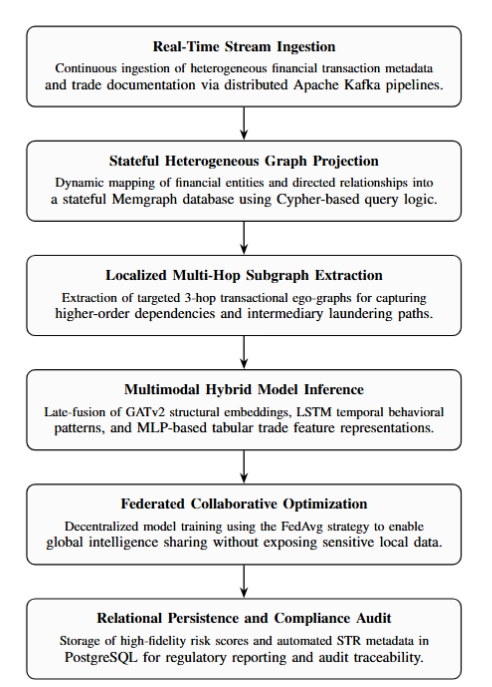
\includegraphics[
        width=\textwidth,
        height=0.8\textheight,
        keepaspectratio
    ]{./Figures/methodology.png}
}
{
    \fbox{
        \parbox[c][0.8\textheight][c]{0.95\textwidth}{
            \centering
            \Large Methodology Diagram Placeholder
        }
    }
}

\caption{Proposed Methodology for TBML Detection}
\label{fig:methodology}
\end{figure}


%========================================================
\section[Assumptions and Constraints of the Work]{\textbf{Assumptions and Constraints of the Work}}
%========================================================

\subsection*{Assumptions}

\begin{itemize}
    \item 
    
It is assumed that the financial transaction records, trade invoices, and customer in
formation utilized for the analysis process are structured, consistent, and preprocessed
in an appropriate manner.
    
    \item 
It is assumed that the involved financial institutions keep their transaction format and
standardized trade attributes similar enough for constructing graphs and analyzing sus
picious activity.
    
    \item 
It is assumed that the created financial datasets include enough normal and suspicious
patterns to learn hidden behavioral relationships between entities for detecting Trade-
Based Money Laundering activities.
    
    \item 
Heterogeneous graph representation is assumed to be capable of describing relations
between different objects including accounts, organizations, transactions, invoices, and
trade entities to detect suspicious financial behavior.
\end{itemize}

\subsection*{Constraints}

\begin{itemize}
    \item 
Evaluation using transactional data of participating financial institutions.
    
    \item 
The performance of the suggested method significantly relies on the quality and com
pleteness of financial datasets available for the training and testing purposes.
    
    \item 
Real-time graph construction and transactional analysis of the huge graph structure
may cause computational and memory overheads in fraud detection operations.
    
    \item 
The framework is verified mainly by means of experimental tests conducted under ac
ademic conditions.
\end{itemize}

\newpage
%========================================================
\section[Organization of the Report]{\textbf{Organization of the Report}}
%========================================================

This report is organized as follows.

\begin{itemize}

    \item 
In Chapter 2, theoretical foundations related to the Trade-Based Money Laundering
detection process, such as anti-money laundering schemes, heterogeneous graph rep
resentation, graph neural networks, and federated learning techniques are introduced.
    
    \item 
    
Chapter 3 demonstrates the Software Requirements Specification (SRS) of the pro
posed framework, which includes functional requirements, system constraints, software
and hardware requirements, and operating procedures.
    
    \item
The general structure of the proposed framework is provided in Chapter 4, where its
architecture, workflow, data flow scheme, and dashboard design are explained.
    
    \item 
Chapter 5 outlines the system design approach that involves constructing heteroge
neous graphs, performing fraud detection, designing STRs, and integrating com
pliance monitoring into the framework.
    
    \item 
Chapter 6 addresses the implementation steps taken during the creation of the pro
posed framework and include data preprocessing, graph construction, back end devel
opment, federated learning algorithm integration, and dashboard construction.
    
    \item 
 Chapter 7 assesses the processes used for testing and validating the proposed frame
work, including functional tests, fraud predictions analysis, dashboard evaluations, and
performance assessment.
    
    \item 
 In Chapter 8, the experimental outcomes and system performance are analyzed in terms
of fraud classification accuracy, scalability, and comprehensive system evaluation
    
    \item 
The ninth chapter provides an overall summary of the conclusions from the suggested work while also analyzing the existing limitations and future improvements of the framework.

\end{itemize}




		
		%Chapter 2
		\chapter{Theory and Fundamentals of Project}

Developing an intelligent framework for Trade-Based Money Laundering detection requires a strong foundation in financial crime analysis, graph theory, and machine learning techniques. This chapter presents the fundamental concepts associated with Trade-Based Money Laundering, Graph Neural Networks, Graph Attention mechanisms, heterogeneous graph representation, and federated learning. The chapter further discusses the computational principles involved in relational transaction modeling, privacy-preserving learning, and real-time fraud analytics. These concepts collectively form the theoretical foundation for the proposed fraud detection framework.

%========================================================
\section[Trade-Based Money Laundering ]{\textbf{Trade-Based Money Laundering }}
%========================================================

\gls{tbml} is a sophisticated form of financial crime in which illicit funds are transferred and concealed through seemingly legitimate international trade activities. Unlike conventional laundering methods that primarily depend on direct financial transactions, TBML exploits import-export systems, trade invoices, shipping documents, and cross-border commercial operations to disguise the movement of illegal funds. Due to the increasing implementation of strict \gls{aml} regulations and \gls{kyc} policies, criminal organizations have increasingly shifted toward trade-oriented laundering mechanisms that are comparatively difficult to detect using traditional monitoring systems.

The complexity of modern global trade ecosystems, combined with the involvement of multiple financial entities and transactional relationships, has made TBML detection a major challenge for financial institutions and regulatory agencies. Consequently, intelligent analytical techniques capable of identifying hidden transactional dependencies and suspicious financial behavior have become increasingly important in modern Anti-Money Laundering systems.

%========================================================
\subsection[Introduction to TBML]{\textbf{Introduction to TBML}}
%========================================================

Trade-Based Money Laundering primarily involves the manipulation of international trade transactions to illegally transfer value between entities located across different countries. Criminal organizations often misuse trade documentation, invoice values, shipment quantities, and commercial agreements to move illicit funds while making the transactions appear legitimate within global financial systems. Since these laundering activities are embedded within regular import-export operations, identifying suspicious behavior becomes highly challenging for financial institutions and regulatory agencies.

In many TBML operations, colluding buyers and sellers intentionally manipulate the declared value of traded goods to transfer illegal financial assets across borders. Techniques such as over invoicing, under invoicing, phantom shipments, and multiple invoicing are commonly used to conceal the movement of illicit proceeds. Such laundering mechanisms exploit the complexity and high transactional volume of international trade systems, making traditional rule-based Anti-Money Laundering approaches comparatively ineffective in detecting hidden financial relationships.

\vspace{0.4cm}
\begin{figure}[H]
\centering
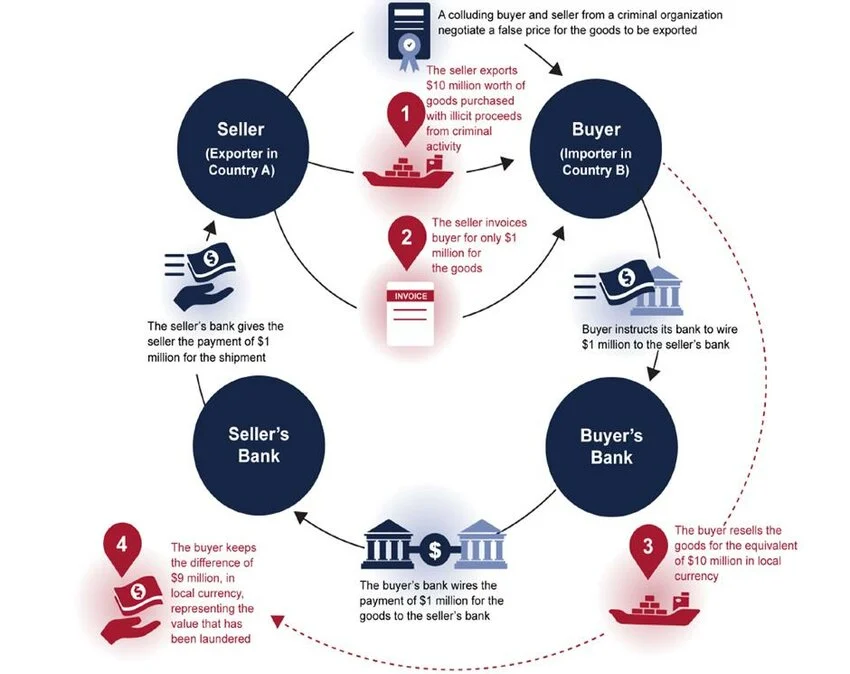
\includegraphics[width=0.82\textwidth]{./Figures/tbmlcycle.png}

\caption{Trade-Based Money Laundering through trade misinvoicing and open-account transactions}
\label{fig:tbml_cycle}

\end{figure}

\vspace{-0.2cm}

\noindent
\textit{Source: Adapted from ``The Role of Misinvoicing in the Money Laundering Cycle,'' 
\href{https://www.researchgate.net/figure/TBML-through-Open-Account-Transactions_fig1_370021180}{ResearchGate}.}

\vspace{0.3cm}

Figure~\ref{fig:tbml_cycle} illustrates a typical Trade-Based Money Laundering workflow involving collusion between exporters and importers across different jurisdictions.

%========================================================
\subsection[Common Techniques Used in TBML]{\textbf{Common Techniques Used in TBML}}
%========================================================

Trade-Based Money Laundering activities are generally performed through the manipulation of trade documentation, shipment details, pricing structures, and financial transactions associated with international trade operations. Criminal organizations exploit the complexity of global trade ecosystems to transfer illicit value across borders while making the transactions appear legitimate. Several laundering techniques are commonly used within modern trade systems to disguise the movement of illegal funds and avoid detection from financial monitoring authorities.

%========================================================
\subsubsection[Over Invoicing]{\textbf{Over Invoicing}}
%========================================================

Over invoicing is a laundering technique in which the value of exported or imported goods is intentionally declared higher than the actual market value. In this process, the buyer transfers an inflated payment amount to the seller, allowing excess funds to be moved across borders under the appearance of legitimate trade transactions. Criminal organizations use this technique to transfer illicit financial assets while avoiding suspicion from conventional banking systems.

%========================================================
\subsubsection[Under Invoicing]{\textbf{Under Invoicing}}
%========================================================

Under invoicing involves declaring a lower value for traded goods when compared to their actual market price. This technique allows the buyer or seller to secretly transfer additional financial value outside formal banking channels. Under invoicing is commonly used to evade taxes, conceal illegal profits, and facilitate hidden movement of illicit assets across jurisdictions.

%========================================================
\subsubsection[Multiple Invoicing]{\textbf{Multiple Invoicing}}
%========================================================

Multiple invoicing refers to the repeated use of the same trade invoice to justify several financial transactions for a single shipment of goods. By duplicating invoices across multiple banking channels or financial institutions, criminal entities can move large amounts of illicit funds while creating the appearance of legitimate trade payments. Detecting such duplicated transactional behavior is challenging in traditional rule-based monitoring systems.

%========================================================
\subsubsection[Phantom Shipments]{\textbf{Phantom Shipments}}
%========================================================

Phantom shipment laundering occurs when financial transactions are conducted for goods that are never actually shipped or delivered. Fraudulent trade documentation and fabricated shipping records are used to create the illusion of legitimate trade activity while transferring illicit funds between colluding entities. Since no physical goods are exchanged, identifying phantom shipment activities requires strong transactional verification and relational analysis mechanisms.

%========================================================
\subsubsection[Misrepresentation of Goods]{\textbf{Misrepresentation of Goods}}
%========================================================

Misrepresentation of goods involves intentionally providing false descriptions regarding the type, quantity, quality, or category of traded products within commercial documents and invoices. Criminal organizations use this technique to manipulate trade valuations and conceal suspicious financial activities under legitimate business transactions. Such inconsistencies are difficult to identify using isolated transactional analysis methods due to the large volume and diversity of international trade operations.

%========================================================
\subsection[Challenges in Detecting TBML]{\textbf{Challenges in Detecting TBML}}
%========================================================

Detecting \gls{tbml} activities is highly challenging due to the complexity and interconnected nature of modern international trade ecosystems. Unlike conventional financial fraud, TBML transactions are often embedded within legitimate commercial operations, making suspicious activities difficult to distinguish from regular trade behavior. Criminal organizations exploit multiple jurisdictions, shell companies, intermediaries, and layered transactional structures to conceal the movement of illicit funds within normal trade systems.

Traditional \gls{aml} systems primarily depend on rule-based monitoring approaches and isolated transactional analysis techniques. Although these systems are capable of identifying predefined suspicious patterns, they often fail to capture hidden relational dependencies among entities involved in large-scale trade networks. The increasing volume of cross-border financial transactions and evolving laundering strategies further reduce the effectiveness of conventional fraud detection mechanisms.

Another major challenge involves institutional privacy and regulatory compliance constraints associated with financial data sharing. Many organizations are unable to directly exchange sensitive transactional information due to confidentiality policies and legal restrictions. Consequently, modern TBML detection systems require intelligent, scalable, and privacy-preserving analytical frameworks capable of modeling complex financial relationships while supporting real-time fraud detection within large trade ecosystems.


\section{Algorithms Used}
\subsection{Graph Attention Network v2 (GATv2)}

\subsubsection{Introduction}

Graph Attention Network v2 (GATv2) is an advanced Graph Neural Network (GNN) architecture designed to improve the attention mechanism used in graph-based deep learning models. It was introduced as an enhancement over the original Graph Attention Network (GAT) to overcome the limitation of static attention and provide a more expressive and dynamic way of learning relationships between nodes in a graph.

GATv2 enables the model to automatically determine the importance of neighboring nodes while updating node representations. This makes it highly effective for applications such as:

\begin{itemize}
    \item Traffic prediction
    \item Social network analysis
    \item Recommendation systems
    \item Molecular property prediction
    \item Fraud detection
    \item Autonomous vehicle navigation
\end{itemize}

Unlike traditional neural networks that work on Euclidean data such as images or sequences, GATv2 is specifically designed to process graph-structured data where relationships between entities are represented as nodes and edges.

\subsubsection{Fundamental Concept of GATv2}

The primary objective of GATv2 is to learn node embeddings by aggregating information from neighboring nodes using an attention mechanism.

For a node \(i\), the model computes:

\begin{enumerate}
    \item Which neighboring nodes are important
    \item How much importance each neighbor should receive
    \item A weighted combination of neighboring features
\end{enumerate}

This process allows the network to dynamically focus on the most relevant neighbors.

\subsubsection{Architecture and Working of GATv2}

The overall architecture and workflow of GATv2 are shown in Figure 1.1.

\begin{figure}[H]
    \centering
    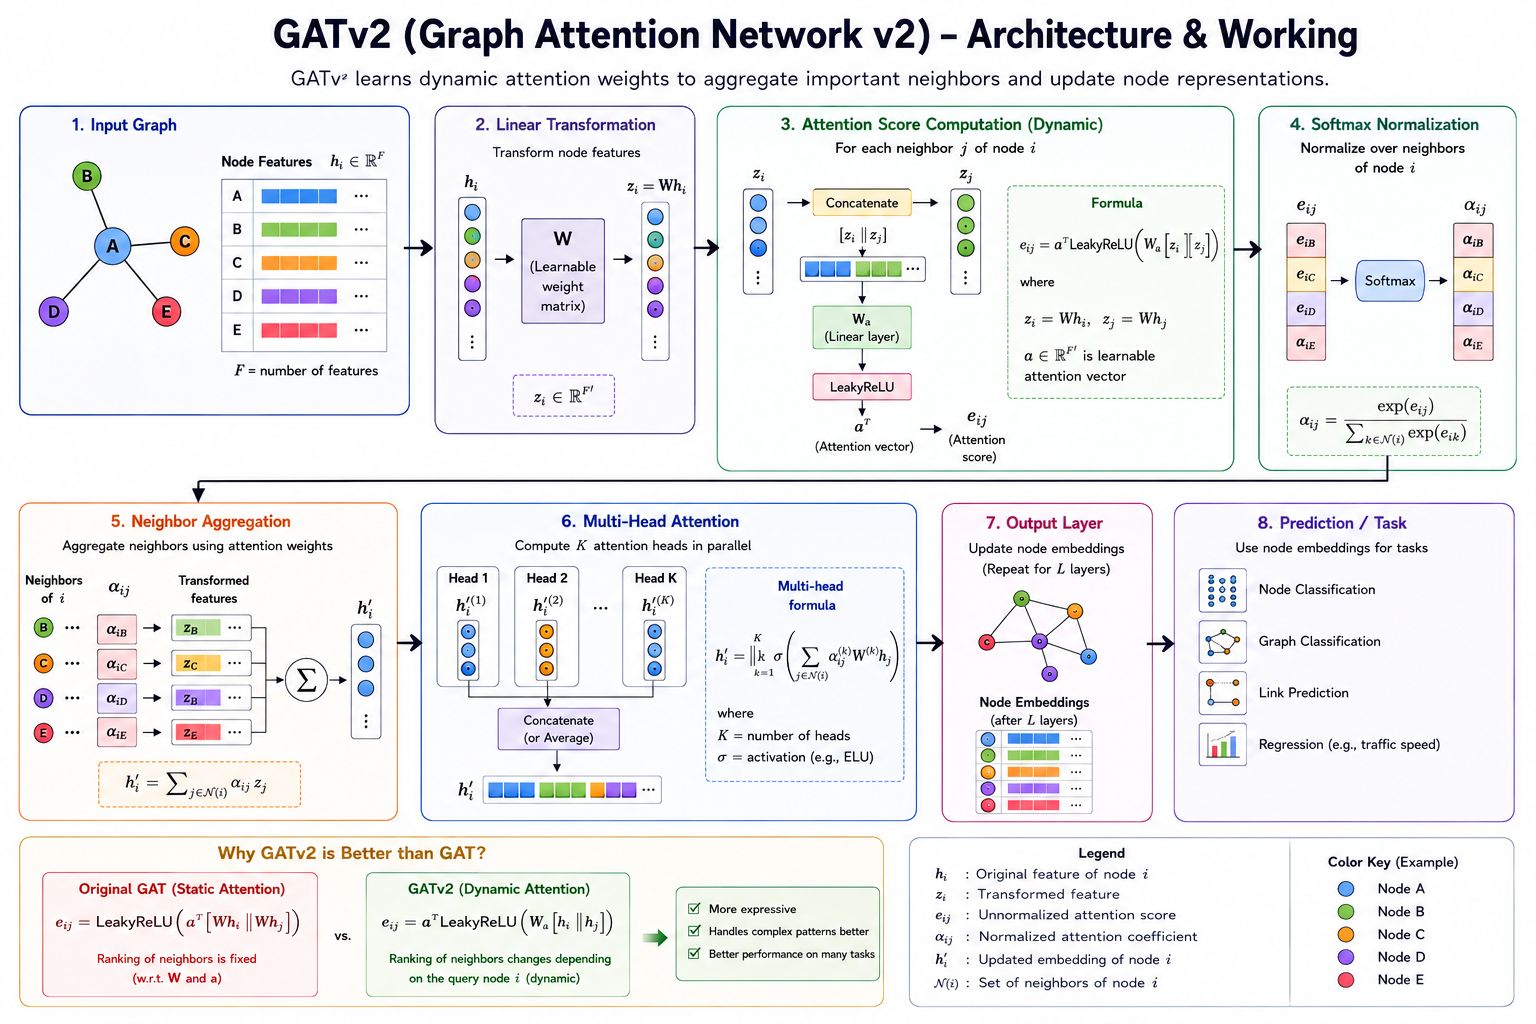
\includegraphics[width=\textwidth]{Figures/GATv2.png}
    \caption{GATv2 Architecture and Working}
    \label{fig:gatv2_architecture}
\end{figure}

The architecture of GATv2 consists of multiple stages including input graph processing, feature transformation, attention computation, normalization, neighbor aggregation, multi-head attention, and prediction generation. Each stage plays a significant role in learning effective graph representations.

\paragraph{Step 1: Input Graph}

The process begins with a graph consisting of nodes, edges, and node feature vectors. Each node contains a feature vector representing its properties.

Mathematically, the node feature vector is represented as:

\[
h_i \in \mathbb{R}^{F}
\]

where:
\begin{itemize}
    \item \(h_i\) represents the feature vector of node \(i\)
    \item \(F\) represents the number of input features
\end{itemize}

In traffic prediction systems, nodes may represent road intersections while edges represent road connectivity. Features may include traffic density, vehicle speed, congestion level, and signal timing information.

\paragraph{Step 2: Linear Transformation}

The input node features are transformed using a learnable weight matrix to extract higher-level representations.

\[
z_i = Wh_i
\]

where:
\begin{itemize}
    \item \(W\) is the learnable weight matrix
    \item \(h_i\) is the original node feature
    \item \(z_i\) is the transformed feature representation
\end{itemize}

This transformation helps the network learn useful combinations of input features and improves feature representation before attention computation.

\paragraph{Step 3: Attention Score Computation}

The attention mechanism is the core component of GATv2. For every connected pair of nodes \((i,j)\), the model computes an attention score representing the importance of neighboring node \(j\) to node \(i\).

The attention mechanism is given by:

\[
e_{ij}=a^{T}\text{LeakyReLU}\left(W[h_i \Vert h_j]\right)
\]

where:
\begin{itemize}
    \item \(h_i\) and \(h_j\) are node feature vectors
    \item \([h_i \Vert h_j]\) represents concatenation
    \item \(W\) is the learnable weight matrix
    \item \(a\) is the learnable attention vector
    \item \(e_{ij}\) is the unnormalized attention score
\end{itemize}

This mechanism dynamically determines the importance of neighboring nodes.

\paragraph{Step 4: Softmax Normalization}

The attention scores are normalized using the softmax function to convert them into probability values.

\[
\alpha_{ij} = \frac{\exp(e_{ij})}{\sum_{k \in \mathcal{N}(i)} \exp(e_{ik})}
\]

where:
\begin{itemize}
    \item \(\alpha_{ij}\) is the normalized attention coefficient
    \item \(\mathcal{N}(i)\) represents the neighboring nodes of node \(i\)
\end{itemize}

This normalization ensures that the attention coefficients sum to 1 and represent the relative importance of neighboring nodes.

\paragraph{Step 5: Neighbor Aggregation}

The neighboring node features are aggregated using weighted summation based on the attention coefficients.

\[
h_i^{\prime} = \sum_{j \in \mathcal{N}(i)} \alpha_{ij}Wh_j
\]

where:
\begin{itemize}
    \item \(h_i^{\prime}\) is the updated node representation
    \item \(\alpha_{ij}\) is the attention coefficient
    \item \(Wh_j\) is the transformed neighboring feature
\end{itemize}

This step allows important neighbors to contribute more significantly to the updated node embedding.

\paragraph{Step 6: Multi-Head Attention}

GATv2 uses multiple attention heads operating in parallel. Each attention head learns different relationships and feature interactions within the graph.

The multi-head attention mechanism is represented as:

\[
h_i^{\prime} =
\mathop{\Vert}_{k=1}^{K}
\sigma
\left(
\sum_{j \in \mathcal{N}(i)}
\alpha_{ij}^{(k)}W^{(k)}h_j
\right)
\]

where:
\begin{itemize}
    \item \(K\) is the number of attention heads
    \item \(\sigma\) is the activation function
    \item \(\Vert\) denotes concatenation
\end{itemize}

Multi-head attention improves learning capability by capturing multiple feature relationships simultaneously.

\paragraph{Step 7: Output Layer and Prediction}

The final node embeddings generated by the attention layers are passed to the output layer for downstream tasks such as:
\begin{itemize}
    \item Node classification
    \item Graph classification
    \item Link prediction
    \item Regression tasks
\end{itemize}

The learned node embeddings contain rich structural and semantic information that helps improve prediction accuracy.

\subsubsection{Advantages of GATv2}

The major advantages of GATv2 are as follows:

\begin{itemize}
    \item Dynamic attention mechanism enables adaptive neighbor importance learning.
    
    \item Improved expressiveness compared to the original GAT architecture.
    
    \item Automatically identifies important neighboring nodes without manual feature engineering.
    
    \item Multi-head attention improves robustness and representation learning.
    
    \item Performs effectively on irregular graph-structured data.
    
    \item Suitable for applications such as traffic prediction, recommendation systems, and autonomous navigation.
\end{itemize}

\subsubsection{Limitations of GATv2}

Despite its advantages, GATv2 also has certain limitations:

\begin{itemize}
    \item Computational complexity increases for large-scale graphs.
    
    \item Requires higher memory consumption due to attention computations.
    
    \item Training time increases with the number of nodes and edges.
    
    \item Deep GATv2 architectures may suffer from over-smoothing problems.
    
    \item Scalability becomes challenging for extremely large graph datasets.
\end{itemize}
\subsubsection{GATv2 vs GAT}

Graph Attention Network v2 (GATv2) was introduced as an improvement over the original Graph Attention Network (GAT) to overcome the limitation of static attention mechanisms. Although both architectures use attention-based aggregation for graph representation learning, GATv2 provides a more expressive and dynamic attention mechanism.

In the original GAT architecture, the ranking of neighboring nodes becomes fixed after the linear transformation step. This limitation reduces the flexibility of the model in learning complex relationships between nodes. The attention mechanism in GAT is given by:

\[
e_{ij} = \text{LeakyReLU}\left(a^{T}[Wh_i \Vert Wh_j]\right)
\]

In GATv2, the order of operations is modified to make the attention mechanism dynamic and more expressive:

\[
e_{ij}=a^{T}\text{LeakyReLU}\left(W[h_i \Vert h_j]\right)
\]

This modification enables the attention scores to depend dynamically on both source and neighboring nodes, allowing the model to learn more meaningful node relationships.

The major differences between GAT and GATv2 are summarized in Table \ref{tab:gat_vs_gatv2}.

\begin{table}[H]
\centering
\caption{Comparison Between GAT and GATv2}
\label{tab:gat_vs_gatv2}
\begin{tabular}{|p{4cm}|p{4.5cm}|p{4.5cm}|}
\hline
\textbf{Feature} & \textbf{GAT} & \textbf{GATv2} \\
\hline
Attention Type & Static Attention & Dynamic Attention \\
\hline
Neighbor Ranking & Fixed after transformation & Changes dynamically based on node context \\
\hline
Expressiveness & Limited & More expressive \\
\hline
Feature Interaction & Moderate & Improved feature interaction learning \\
\hline
Learning Capability & Lower compared to GATv2 & Better representation learning \\
\hline
Performance & Good & Improved performance on many graph tasks \\
\hline
Flexibility & Less flexible & More adaptive and flexible \\
\hline
\end{tabular}
\end{table}

GATv2 is preferred over GAT because it provides a more powerful and adaptive attention mechanism capable of learning complex graph relationships more effectively. The dynamic attention mechanism allows the model to assign different importance values to neighboring nodes depending on the context of the current node. This improves feature aggregation, representation learning, and prediction accuracy.

Due to these advantages, GATv2 is widely preferred in modern graph-based applications such as traffic prediction, autonomous vehicle navigation, recommendation systems, and social network analysis.


\subsection{Long Short-Term Memory (LSTM)}

\subsubsection{Introduction to LSTM}

Shortly after the first Elman-style Recurrent Neural Networks (RNNs) were trained using backpropagation, researchers observed a major limitation in learning long-term dependencies. This problem mainly occurred because of:

\begin{itemize}
    \item Vanishing gradients
    \item Exploding gradients
\end{itemize}

Although gradient clipping could help reduce exploding gradients, handling vanishing gradients required a more advanced solution. To solve this issue, Hochreiter and Schmidhuber introduced the Long Short-Term Memory (LSTM) architecture in 1997.

Unlike standard RNNs, where each recurrent node simply passes information to the next time step, LSTMs introduce a special structure called a memory cell. This memory cell maintains an internal state that allows information to persist over many time steps without vanishing.

The key idea behind LSTM is the ability to:

\begin{itemize}
    \item Remember important information
    \item Forget irrelevant information
    \item Control the flow of information through gates
\end{itemize}

This enables LSTMs to learn long-term sequential dependencies effectively.

\subsubsection{Gated Memory Cell}

Each memory cell is equipped with an internal state and a number of multiplicative gates that determine whether:
\begin{enumerate}
    \item A given input should impact the internal state (the input gate),
    \item The internal state should be flushed to 0 (the forget gate), and
    \item The internal state of a given neuron should be allowed to impact the cell’s output (the output gate).
\end{enumerate}

\subsubsection{Gated Hidden State}

The key distinction between vanilla RNNs and LSTMs is that the latter support gating of the hidden state. This means that we have dedicated mechanisms for when a hidden state should be updated and also for when it should be reset. These mechanisms are learned and they address the concerns listed above. For instance, if the first token is of great importance we will learn not to update the hidden state after the first observation. Likewise, we will learn to skip irrelevant temporary observations. Last, we will learn to reset the latent state whenever needed. We discuss this in detail below.

\subsubsection{Input Gate, Forget Gate, and Output Gate}

The data feeding into the LSTM gates are the input at the current time step and the hidden state of the previous time step, as illustrated in Fig.~10.1.1. Three fully connected layers with sigmoid activation functions compute the values of the input, forget, and output gates. As a result of the sigmoid activation, all values of the three gates are in the range of $(0,1)$.

Additionally, we require an input node, typically computed with a \texttt{tanh} activation function. Intuitively, the input gate determines how much of the input node’s value should be added to the current memory cell internal state. The forget gate determines whether to keep the current value of the memory or flush it. The output gate determines whether the memory cell should influence the output at the current time step.

\begin{figure}[H]
    \centering
    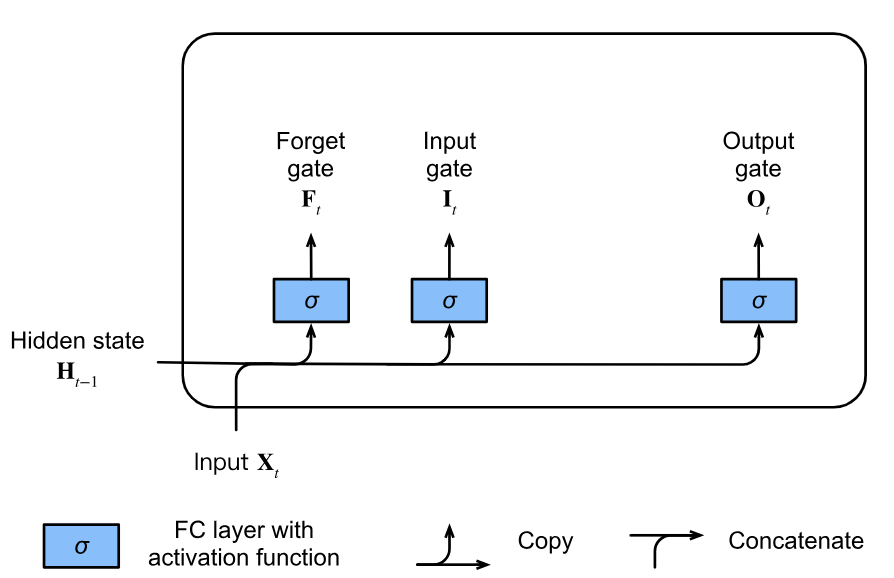
\includegraphics[width=0.7\textwidth]{Figures/LSTM_0}
    \caption{Computing the input gate, the forget gate, and the output gate in an LSTM model}
    \label{fig:lstm_gates}
\end{figure}

Mathematically, suppose that there are $h$ hidden units, the batch size is $n$, and the number of inputs is $d$. Thus, the input is $\mathbf{X}_t \in \mathbb{R}^{n \times d}$ and the hidden state of the previous time step is $\mathbf{H}_{t-1} \in \mathbb{R}^{n \times h}$.

Correspondingly, the gates at time step $t$ are defined as follows: the input gate is $\mathbf{I}_t \in \mathbb{R}^{n \times h}$, the forget gate is $\mathbf{F}_t \in \mathbb{R}^{n \times h}$, and the output gate is $\mathbf{O}_t \in \mathbb{R}^{n \times h}$. They are calculated as follows:

\begin{equation}
\begin{aligned}
\mathbf{I}_t &= \sigma(\mathbf{X}_t \mathbf{W}_{\textrm{xi}} + \mathbf{H}_{t-1} \mathbf{W}_{\textrm{hi}} + \mathbf{b}_{\textrm{i}}),\\
\mathbf{F}_t &= \sigma(\mathbf{X}_t \mathbf{W}_{\textrm{xf}} + \mathbf{H}_{t-1} \mathbf{W}_{\textrm{hf}} + \mathbf{b}_{\textrm{f}}),\\
\mathbf{O}_t &= \sigma(\mathbf{X}_t \mathbf{W}_{\textrm{xo}} + \mathbf{H}_{t-1} \mathbf{W}_{\textrm{ho}} + \mathbf{b}_{\textrm{o}})
\end{aligned}
\end{equation}

where $\mathbf{W}_{\textrm{xi}}, \mathbf{W}_{\textrm{xf}}, \mathbf{W}_{\textrm{xo}} \in \mathbb{R}^{d \times h}$ and $\mathbf{W}_{\textrm{hi}}, \mathbf{W}_{\textrm{hf}}, \mathbf{W}_{\textrm{ho}} \in \mathbb{R}^{h \times h}$ are weight parameters and $\mathbf{b}_{\textrm{i}}, \mathbf{b}_{\textrm{f}}, \mathbf{b}_{\textrm{o}} \in \mathbb{R}^{1 \times h}$ are bias parameters.

Note that broadcasting is triggered during the summation. We use sigmoid functions to map the input values to the interval $(0,1)$.

\subsubsection{Input Node}

Next we design the memory cell. Since we have not specified the action of the various gates yet, we first introduce the input node $\tilde{\mathbf{C}}_t \in \mathbb{R}^{n \times h}$. Its computation is similar to that of the three gates described above, but uses a \texttt{tanh} function with a value range for $(-1,1)$ as the activation function. This leads to the following equation at time step $t$:

\begin{equation}
\tilde{\mathbf{C}}_t = \textrm{tanh}(\mathbf{X}_t \mathbf{W}_{\textrm{xc}} + \mathbf{H}_{t-1} \mathbf{W}_{\textrm{hc}} + \mathbf{b}_{\textrm{c}})
\end{equation}

where $\mathbf{W}_{\textrm{xc}} \in \mathbb{R}^{d \times h}$ and $\mathbf{W}_{\textrm{hc}} \in \mathbb{R}^{h \times h}$ are weight parameters and $\mathbf{b}_{\textrm{c}} \in \mathbb{R}^{1 \times h}$ is a bias parameter.

A quick illustration of the input node is shown in Fig.~10.1.2.

\begin{figure}[H]
    \centering
    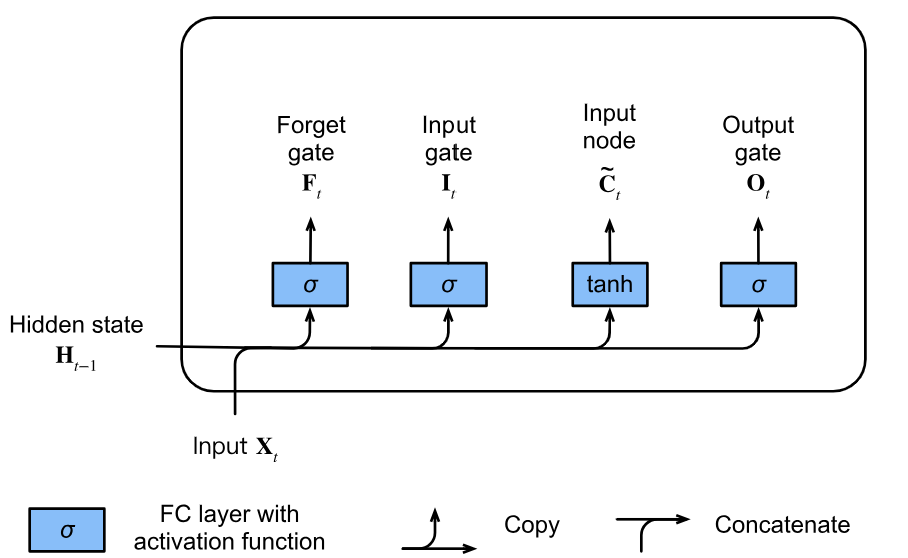
\includegraphics[width=0.7\textwidth]{Figures/LSTM_1}
    \caption{Computing the input node in an LSTM model}
    \label{fig:lstm_input_node}
\end{figure}

\subsubsection{Memory Cell Internal State}

In LSTMs, the input gate $\mathbf{I}_t$ governs how much we take new data into account via $\tilde{\mathbf{C}}_t$ and the forget gate $\mathbf{F}_t$ addresses how much of the old cell internal state $\mathbf{C}_{t-1} \in \mathbb{R}^{n \times h}$ we retain. Using the Hadamard (elementwise) product operator $\odot$ we arrive at the following update equation:

\begin{equation}
\mathbf{C}_t = \mathbf{F}_t \odot \mathbf{C}_{t-1} + \mathbf{I}_t \odot \tilde{\mathbf{C}}_t
\end{equation}

If the forget gate is always 1 and the input gate is always 0, the memory cell internal state $\mathbf{C}_{t-1}$ will remain constant forever, passing unchanged to each subsequent time step. However, input gates and forget gates give the model the flexibility of being able to learn when to keep this value unchanged and when to perturb it in response to subsequent inputs.

In practice, this design alleviates the vanishing gradient problem, resulting in models that are much easier to train, especially when facing datasets with long sequence lengths.

We thus arrive at the flow diagram in Fig.~10.1.3.

\begin{figure}[H]
    \centering
    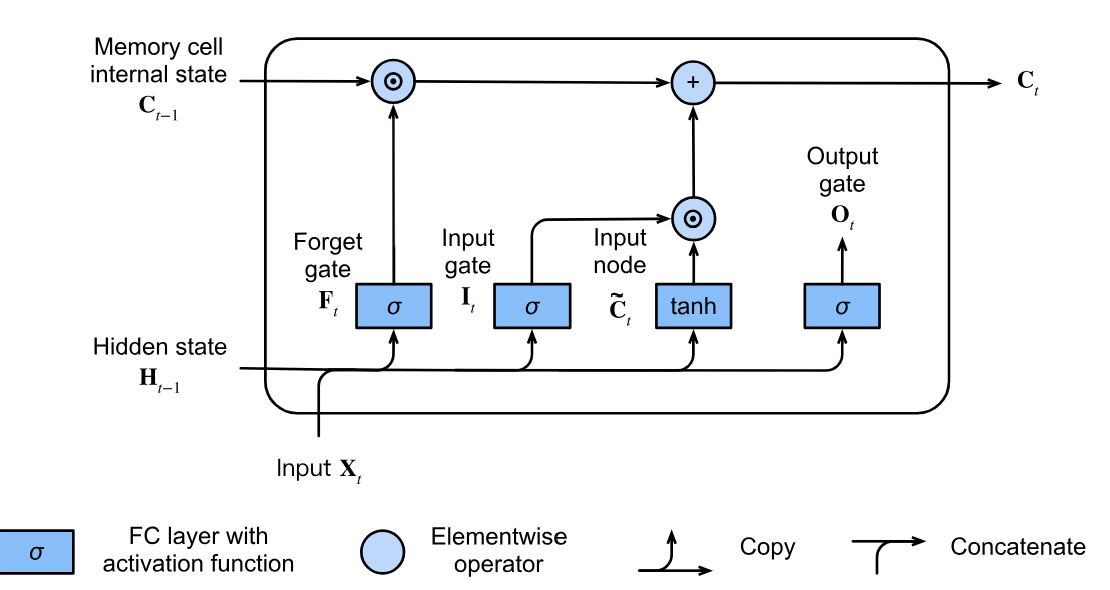
\includegraphics[width=0.7\textwidth]{Figures/LSTM_2}
    \caption{Computing the memory cell internal state in an LSTM model}
    \label{fig:lstm_memory_cell}
\end{figure}

\subsubsection{Hidden State}

Last, we need to define how to compute the output of the memory cell, i.e., the hidden state $\mathbf{H}_t \in \mathbb{R}^{n \times h}$, as seen by other layers. This is where the output gate comes into play.

In LSTMs, we first apply \texttt{tanh} to the memory cell internal state and then apply another point-wise multiplication, this time with the output gate. This ensures that the values of $\mathbf{H}_t$ are always in the interval $(-1,1)$:

\begin{equation}
\mathbf{H}_t = \mathbf{O}_t \odot \tanh(\mathbf{C}_t)
\end{equation}

Whenever the output gate is close to 1, we allow the memory cell internal state to impact the subsequent layers uninhibited, whereas for output gate values close to 0, we prevent the current memory from impacting other layers of the network at the current time step.

Note that a memory cell can accrue information across many time steps without impacting the rest of the network (as long as the output gate takes values close to 0), and then suddenly impact the network at a subsequent time step as soon as the output gate flips from values close to 0 to values close to 1.

Fig.~10.1.4 has a graphical illustration of the data flow.

\begin{figure}[H]
    \centering
    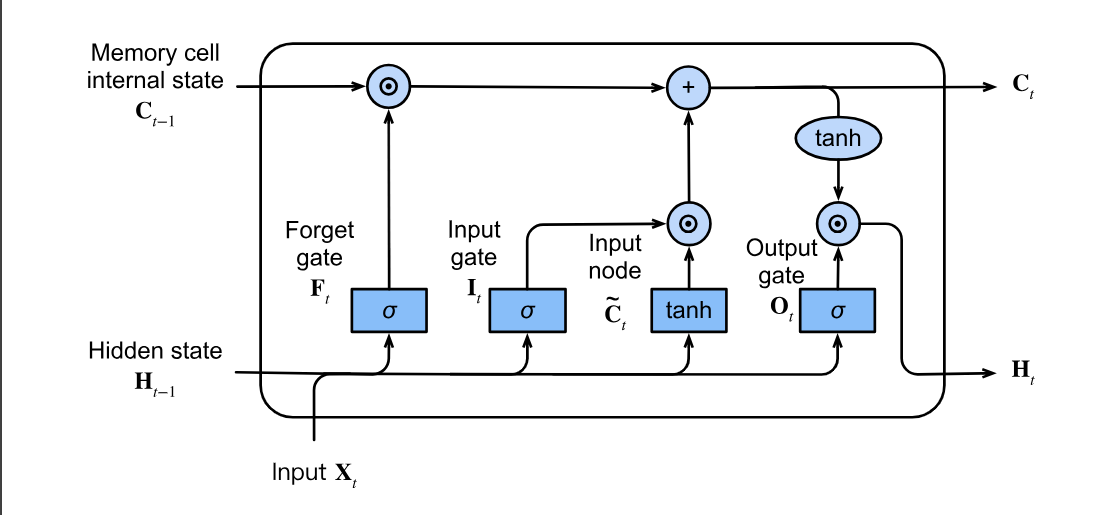
\includegraphics[width=0.7\textwidth]{Figures/LSTM_3}
    \caption{Computing the hidden state in an LSTM model}
    \label{fig:lstm_hidden_state}
\end{figure}

\subsubsection{Advantages of LSTM}

The major advantages of LSTM are as follows:

\begin{itemize}
    \item LSTM effectively solves the vanishing gradient problem faced by traditional Recurrent Neural Networks (RNNs).
    
    \item It can learn long-term dependencies and preserve information over extended sequence lengths.
    
    \item The gating mechanism enables selective memory retention and controlled information flow.
    
    \item LSTM performs well on sequential and time-series data.
    
    \item It is highly effective in applications such as natural language processing, speech recognition, machine translation, traffic prediction, and stock market forecasting.
    
    \item The memory cell architecture allows important information to persist across multiple time steps.
    
    \item LSTM networks are more stable and easier to train compared to vanilla RNNs.
\end{itemize}

\subsubsection{Limitations of LSTM}

Despite its advantages, LSTM also has certain limitations:

\begin{itemize}
    \item LSTM networks are computationally expensive due to the presence of multiple gates and memory cells.
    
    \item Training LSTM models requires high computational power and longer training time.
    
    \item The architecture is more complex compared to traditional RNNs.
    
    \item LSTMs require a large amount of training data for better generalization.
    
    \item They may suffer from overfitting when trained on small datasets.
    
    \item Parallel processing is difficult because sequential data must be processed step-by-step.
    
    \item For extremely long sequences, performance may still degrade despite improved memory retention.
\end{itemize}

\textit{Source: Adapted from ``Dive into Deep Learning,Long Short-Term Memory \href{https://d2l.ai/chapter_recurrent-modern/lstm.html?utm_source=chatgpt.com}{(LSTM)}."}

\vspace{0.3cm}





%========================================================
\section{User Interface}
%========================================================

Modern financial monitoring platforms increasingly rely on scalable web application technologies to support real-time transaction analysis, fraud monitoring, and interactive visualization of financial activities. The rapid growth of digital banking and online financial services has significantly increased the demand for responsive, secure, and data-driven monitoring systems capable of handling large volumes of transactional information efficiently. Consequently, modern Anti-Money Laundering systems employ component-based web architectures and client-server communication models to provide efficient user interaction and real-time analytical capabilities.

Advanced frontend frameworks and backend service architectures play a critical role in enabling modular application development, dynamic rendering, secure authentication, and seamless integration with fraud detection engines. Such technologies support the visualization of suspicious transactional activities, alert generation, role-based access control, and automated compliance workflows within financial institutions. The integration of scalable user interface technologies with intelligent analytical systems further enhances operational efficiency and supports real-time financial crime investigation processes.

%========================================================
\subsection[Modern Web Application Frameworks]{\textbf{Modern Web Application Frameworks}}
%========================================================

Modern web application frameworks provide the architectural foundation required for developing scalable, responsive, and interactive software systems. Traditional web applications primarily relied on static page rendering and tightly coupled server-side architectures, which limited dynamic user interaction and real-time data processing capabilities. In contrast, modern frameworks adopt component-based and asynchronous rendering approaches that improve application scalability, maintainability, and user experience within large-scale distributed systems.

Frontend frameworks such as React.js enable the development of reusable and modular user interface components capable of dynamically updating application states without requiring complete page reloads. Such frameworks employ virtual Document Object Model (DOM) mechanisms and state-driven rendering principles to efficiently manage user interactions and real-time data visualization. This architectural approach significantly improves responsiveness and enables scalable dashboard development for data-intensive applications such as financial monitoring systems.

Server-side rendering and hybrid rendering frameworks such as Next.js further enhance modern web application performance by combining client-side interactivity with optimized server-side content delivery. These frameworks support efficient routing, dynamic data fetching, and improved application scalability while reducing rendering overhead for large-scale systems. Consequently, modern web application frameworks have become an essential foundation for building secure, scalable, and real-time financial monitoring platforms.

%========================================================
\subsection[Component Lifecycle and Reactivity]{\textbf{Component Lifecycle and Reactivity}}
%========================================================

Modern web application frameworks employ reactive rendering mechanisms to dynamically synchronize the user interface with application data and user interactions. In component-based architectures such as React and Next.js, the user interface continuously responds to changes in application state, backend responses, and client-side events. This reactive behavior enables efficient rendering of dynamic content while improving scalability, responsiveness, and maintainability within large-scale financial monitoring systems.

The component lifecycle in modern React and Next.js applications generally follows a sequence of rendering, interaction, updating, and cleanup stages. These stages collectively manage how components are initialized, rendered, updated, and removed during application execution. The overall lifecycle flow can be summarized as follows:

\begin{itemize}

\item \textbf{Server-Side Rendering:}  
Initially, application components are rendered within the server environment where data fetching and content generation are performed before transmitting the rendered output to the client browser. This approach improves initial loading performance and reduces unnecessary client-side computational overhead.

\item \textbf{Hydration and Client Initialization:}  
After the rendered HTML content reaches the client browser, React hydrates the interface by attaching event listeners and enabling interactive functionalities within client-side components. During this stage, local states, dynamic properties, and asynchronous operations are initialized for user interaction.

\item \textbf{Reactive State Updates:}  
As users interact with the application, component states and properties continuously change according to system events and backend responses. React employs Virtual DOM reconciliation mechanisms to compare interface changes and selectively update only the affected components instead of re-rendering the complete application interface.

\item \textbf{Re-rendering and Synchronization:}  
Whenever state transitions occur, the framework dynamically re-renders the modified components and synchronizes the updated data with the user interface. This reactive rendering process enables real-time visualization of financial transactions, fraud alerts, and monitoring analytics within Anti-Money Laundering dashboards.

\item \textbf{Unmounting and Resource Cleanup:}  
When components are removed from the active interface, allocated resources, subscriptions, and temporary states are released to maintain application stability and efficient memory utilization.

\end{itemize}

Such lifecycle management principles are essential in modern financial monitoring platforms where continuous transactional updates, alert generation, and real-time analytical visualization must be processed efficiently while ensuring scalable and responsive user interaction.



%========================================================
\subsection[Data Visualization and Monitoring Dashboards]{\textbf{Data Visualization and Monitoring Dashboards}}
%========================================================

Understanding the theoretical aspects of data visualization is important for analyzing large volumes of financial transactions and interpreting suspicious transactional behavior within real-time monitoring systems. Visualization of analytical outputs enables financial institutions and compliance analysts to identify fraud patterns, transaction anomalies, risk distributions, and suspicious entity relationships more efficiently when compared with conventional tabular analysis methods. Interactive monitoring dashboards further improve situational awareness by enabling continuous observation of fraud alerts, transaction flows, and compliance activities without interrupting real-time analytical processes.

This work conceptualizes financial monitoring and fraud visualization through a web-based dashboard architecture developed using modern frontend technologies and analytical visualization frameworks:

\begin{itemize}

\item \textbf{Nextjs} is employed as the frontend framework for developing responsive and modular user interface components capable of supporting scalable financial monitoring applications.

\item \textbf{Recharts} is utilized for visualizing transactional analytics, fraud classifications, risk score distributions, and temporal financial trends through interactive line graphs, bar charts, pie charts, and statistical dashboards.

\item \textbf{Role-based dashboard interfaces} enable controlled access to monitoring functionalities, fraud investigation workflows, Suspicious Transaction Report (STR) generation, and real-time alert visualization according to user privileges and institutional responsibilities.

\item \textbf{Interactive analytical panels} support continuous monitoring of suspicious activities, transaction histories, and fraud prediction results generated by intelligent detection systems operating within the platform.

\end{itemize}

Modern visualization systems additionally support notification mechanisms, analytical filtering, and export functionalities that assist investigators and compliance officers in conducting financial analysis and generating compliance reports for further examination. The detailed implementation and integration of these visualization technologies within the proposed TBML detection framework are discussed further in the system implementation chapter.


\section*{Summary}

In this chapter, the theoretical foundations required for understanding the proposed Trade-Based Money Laundering detection framework were presented. The chapter began with an introduction to Trade-Based Money Laundering mechanisms and common laundering techniques, establishing the financial and transactional context in which illicit fund movement occurs within international trade ecosystems.

The chapter further explored the challenges associated with detecting suspicious trade activities using conventional Anti-Money Laundering approaches. Concepts related to graph-based financial modeling, heterogeneous graph representation, Graph Neural Networks, Graph Attention mechanisms, and federated learning were discussed to provide the analytical and computational foundation required for intelligent and privacy-preserving fraud detection systems.

Finally, the chapter introduced the concepts associated with modern financial monitoring interfaces, reactive web architectures, and real-time data visualization systems used for fraud analytics and compliance monitoring. The theoretical concepts discussed throughout this chapter provide the foundation for understanding the system architecture, implementation methodologies, and analytical workflows presented in the subsequent chapters.
		
		% Chapter 3
		%========================================================
\chapter{Design of the Proposed TBML Detection Framework}
%========================================================

This chapter presents the design of the proposed \gls{tbml} detection framework. It brings together the software requirements, overall architecture, and module-level design, then walks through the operational requirements and user roles, the system workflows, graph-construction approach, federated learning setup, data-flow representations, and the analytical modules used for detection, investigation, and reporting.

% =====================================
\section{Software Requirements Specifications}
% ========================================================

The software requirements for the proposed TBML detection framework describe what the system needs in order to operate reliably in a real institutional setting. They cover the functional behavior of the platform, the quality attributes it must maintain, the software stack it depends on, and the hardware resources needed to support fraud analysis, transaction monitoring, secure access, and compliance management. The details are grouped into functional requirements, non-functional requirements, software requirements, and hardware requirements in the following subsections.
%========================================================
\subsection[Overall Description]{\textbf{Overall Description}}
%========================================================

The proposed framework is built as a privacy-preserving financial monitoring platform for identifying suspicious Trade-Based Money Laundering activity across large-scale transactional ecosystems. It combines heterogeneous graph-learning mechanisms, federated analytical workflows, role-based monitoring dashboards, and automated Suspicious Transaction Report (STR) generation within a centralized compliance-monitoring environment. In practice, the framework supports real-time transaction monitoring, graph-based fraud classification, institutional investigation workflows, and regulator-side analytical visualization for exposing hidden laundering relationships across connected financial networks.

%========================================================
\subsubsection[Product Perspective]{\textbf{Product Perspective}}
%========================================================
The proposed TBML detection framework acts as a financial monitoring and fraud-analysis platform that brings heterogeneous graph modeling, Graph Neural Network-based analytics, federated learning, and compliance monitoring into one environment. It represents financial entities such as accounts, organizations, invoices, and transactions as connected graph structures so that hidden relationships and suspicious laundering patterns can be captured more effectively than with conventional rule-based Anti-Money Laundering systems. Role-based dashboards are also included to support transaction monitoring, fraud review, alert management, and automated Suspicious Transaction Report (STR) generation.
%========================================================
\subsubsection[Product Functions]{\textbf{Product Functions}}
%========================================================

The primary functionalities supported by the proposed framework are summarized as follows:

\begin{itemize}

\item \textbf{Transaction Monitoring:}  
The system continuously monitors financial transactions and trade-related activities to identify suspicious transactional behavior within large-scale financial ecosystems.

\item \textbf{Graph-Based Financial Analysis:}  
Financial entities such as accounts, organizations, invoices, and transactions are represented as interconnected graph structures for relational analysis and hidden dependency detection.

\item \textbf{Fraud Classification and Risk Prediction:}  
Graph Neural Network-based analytical models classify suspicious transactions and generate fraud risk predictions based on transactional relationships and behavioral patterns.

\item \textbf{Federated Learning Support:}  
The framework supports collaborative model training across multiple institutional environments while preserving sensitive financial data privacy.

\item \textbf{Real-Time Dashboard Visualization:}  
Interactive monitoring dashboards provide visualization of transaction analytics, fraud alerts, risk distributions, and suspicious activity summaries for compliance analysts.

\item \textbf{Suspicious Transaction Report (STR) Generation:}  
The system automatically generates structured Suspicious Transaction Reports for identified fraudulent transactions to support compliance and regulatory workflows.

\item \textbf{Authentication and Role-Based Access Control:}  
Secure authentication and controlled access mechanisms are incorporated to manage user privileges and protect sensitive financial information within the monitoring platform.

\end{itemize}


%========================================================
\subsubsection[User Characteristics]{\textbf{User Characteristics}}
%========================================================

The proposed TBML detection framework supports multiple categories of institutional users involved in fraud monitoring, compliance verification, and regulatory supervision activities. Since the system processes sensitive transactional and compliance-related information, role-based access mechanisms are enforced to ensure secure and controlled interaction with the platform. The major user categories associated with the proposed framework are summarized as follows:

\begin{itemize}

\item \textbf{Bank Compliance Team:}  
The bank compliance team represents institutional analysts responsible for monitoring transactional activities and investigating suspicious financial behavior identified by the fraud-detection framework. These users are expected to possess domain knowledge related to Anti-Money Laundering (AML) procedures, transaction analysis, and institutional compliance operations. Authorized compliance personnel interact with analytical dashboards, review suspicious transaction records, verify fraud alerts, and manage institutional STR escalation workflows.

\item \textbf{Regulatory Administrator:}  
The regulatory administrator functions as a supervisory authority responsible for overseeing fraud-monitoring activities across participating financial institutions. These users typically possess advanced regulatory and compliance expertise associated with financial investigation and institutional auditing operations. Regulatory administrators access consolidated Suspicious Transaction Reports (STRs), monitor institution-level compliance activities, and supervise large-scale suspicious transactional behavior across distributed banking environments.

\end{itemize}




%========================================================
\subsubsection[Constraints]{\textbf{Constraints}}
%========================================================

The development and deployment of the proposed TBML detection framework are subject to multiple operational, computational, and regulatory constraints associated with financial monitoring systems. These limitations influence the scalability, analytical performance, and real-time operational capabilities of the framework.

The major constraints associated with the proposed system are summarized as follows:

\begin{itemize}

\item \textbf{Data Privacy and Regulatory Constraints:}  
Financial institutions operate under strict privacy regulations and compliance policies that restrict direct sharing of sensitive transactional information across organizations.

\item \textbf{Large-Scale Transactional Data Processing:}  
The system must process large volumes of interconnected financial transactions and graph relationships, which may increase computational complexity and memory utilization during real-time analysis.

\item \textbf{Availability of Real-World TBML Datasets:}  
Access to publicly available Trade-Based Money Laundering datasets is limited due to confidentiality and regulatory restrictions, making large-scale real-world experimentation challenging.

\item \textbf{Dynamic Fraud Patterns:}  
Money laundering strategies continuously evolve over time, requiring fraud detection models to adapt to changing transactional behaviors and emerging laundering techniques.

\item \textbf{Infrastructure and Computational Limitations:}  
Training graph-based machine learning models and processing heterogeneous financial networks require significant computational resources, especially for large-scale transactional ecosystems.

\end{itemize}

%========================================================
\subsection[Specific Requirements]{\textbf{Specific Requirements}}
%========================================================

The specific requirements define the operational behavior, performance expectations, software dependencies, and computational resources needed for the framework to run efficiently. They make sure the system can support real-time fraud analysis, scalable monitoring, secure interaction, and intelligent compliance management within financial institutions.

%========================================================
\subsubsection[Functional Requirements]{\textbf{Functional Requirements}}
%========================================================

The functional requirements define the major operations and services that must be supported by the proposed TBML detection framework. The primary functional requirements of the system are summarized as follows:


\begin{itemize}


\item The system shall enforce role-based authorization policies to regulate operational access privileges for compliance analysts and regulatory administrators.

\item The framework shall support ingestion and preprocessing of transactional datasets for heterogeneous financial graph construction.

\item The proposed system shall model financial entities, transactions, and trade relationships as interconnected heterogeneous graph structures.

\item The analytical engine shall perform graph-based fraud classification and generate transaction-level risk predictions using federated learning methodologies.

\item The dashboard infrastructure shall support real-time visualization of suspicious transactions, fraud alerts, analytical summaries, and compliance-monitoring activities.

\item The system shall enable institutional compliance teams to review suspicious transactions and perform fraud escalation or clearance procedures.

\item The framework shall provide features to generate Suspicious Transaction Reports (STRs) for transactions identified as potentially fraudulent.

\item The regulator-side monitoring interface shall support centralized supervision of institutional fraud reports and suspicious financial activities.

\item The analytical interface shall provide transaction-filtering, search, and investigative querying functionalities for fraud-analysis workflows.


\end{itemize}





%========================================================
\subsubsection[Non-Functional Requirements]{\textbf{Non-Functional Requirements}}
%========================================================

The non-functional requirements define the quality attributes, operational constraints, and performance expectations associated with the proposed TBML detection framework. These requirements ensure that the system remains scalable, secure, reliable, and responsive while processing large-scale financial transactions and analytical workloads.

The primary non-functional requirements associated with the proposed system are summarized as follows:

\begin{itemize}

\item \textbf{Scalability:}  
The framework should support scalable processing of large transactional datasets and heterogeneous graph structures without significant degradation in analytical performance.

\item \textbf{Real-Time Processing:}  
The system should support low-latency transaction analysis and fraud prediction to enable continuous real-time monitoring of suspicious financial activities.

\item \textbf{Security and Privacy:}  
The framework should ensure secure access control, protected communication, and privacy-preserving handling of sensitive financial information and compliance-related data.

\item \textbf{Reliability:}  
The system should maintain stable analytical performance and continuous monitoring capabilities during prolonged operational workloads and concurrent user access.

\item \textbf{Availability:}  
The monitoring platform should provide consistent access to dashboards, fraud analytics, and reporting services for authorized institutional users.

\item \textbf{Maintainability:}  
The system architecture should support modular development, efficient debugging, and simplified integration of additional analytical modules and monitoring functionalities.

\item \textbf{Usability:}  
The dashboard interfaces and visualization systems should provide intuitive interaction mechanisms for compliance analysts and regulatory administrators during fraud investigation activities.

\end{itemize}


%========================================================
\subsubsection[Software Requirements]{\textbf{Software Requirements}}
%========================================================

The implementation of the proposed TBML detection framework depends on a combination of software technologies, machine learning libraries, backend services, database systems, and visualization tools. Together, these components support graph-based fraud detection, federated learning, real-time transaction monitoring, and compliance management. The framework therefore needs coordinated interaction between the frontend dashboard, backend processing services, database layers, and machine learning environments. The software requirements are summarized in Table~\ref{tab:software_requirements}.
\vspace{0.3cm}

\footnotesize
\renewcommand{\arraystretch}{1.5}

\begin{table}[H]

\caption{Software Requirements of the Proposed TBML Detection Framework}
\label{tab:software_requirements}

\vspace{0.2cm}

\centering

\begin{tabular}{|p{3.5cm}|p{4.2cm}|p{5.8cm}|}

\hline
\textbf{Category} & \textbf{Technologies / Tools} & \textbf{Purpose in the System} \\
\hline

Operating System 
& Windows 11 
& Provides the development and deployment environment for backend services, databases, and analytical modules. \\
\hline

Programming Languages 
& Python, JavaScript 
& Used for backend development, machine learning workflows, API services, and frontend application development. \\
\hline

Frontend Frameworks 
& Next.js, React.js, Tailwind CSS 
& Supports responsive user interface development, dashboard visualization, and real-time monitoring functionalities. \\
\hline

Backend Framework 
& FastAPI 
& Facilitates asynchronous API communication between frontend dashboards and backend fraud detection services. \\
\hline

Database Systems 
& PostgreSQL, Memgraph 
& Stores transactional records, graph relationships, compliance information, and analytical data required for fraud analysis. \\
\hline

Machine Learning Frameworks 
& PyTorch, PyTorch Geometric 
& Supports deep learning operations, Graph Neural Network implementation, and graph-driven fraud analysis. \\
\hline

Federated Learning Framework 
& Flower 
& Enables distributed federated learning and privacy-preserving model aggregation across institutional environments. \\
\hline

Streaming Platform 
& Apache Kafka 
& Supports real-time transaction streaming and event-driven processing within the monitoring pipeline. \\
\hline

Containerization Platform 
& Docker 
& Provides containerized deployment and scalable execution environments for system integration. \\
\hline

LLM Integration Service 
& Groq LLM API 
& Supports automated generation of Suspicious Transaction Reports and compliance-oriented analytical summaries. \\
\hline

\end{tabular}

\end{table}

\normalsize
%========================================================
\subsubsection[Hardware Requirements]{\textbf{Hardware Requirements}}
%========================================================

The implementation of the proposed TBML detection framework also needs a defined hardware setup to support graph processing, machine learning execution, federated coordination, real-time transaction monitoring, and dashboard visualization. The required hardware is summarized in Table~\ref{tab:hardware_requirements}.

\vspace{0.3cm}

\footnotesize
\renewcommand{\arraystretch}{1.4}

\begin{table}[H]


\caption{Hardware Requirements of the Proposed TBML Detection Framework}
\label{tab:hardware_requirements}

\vspace{0.2cm}

\centering

\begin{tabular}{|p{3.0cm}|p{2.6cm}|p{8.0cm}|}

\hline
\textbf{Hardware Component} & \textbf{Minimum Requirement} & \textbf{Purpose in the System} \\
\hline

Processor & Intel Core i7 / AMD Ryzen 7 & Supports efficient execution of graph analytical models, backend services, and machine learning computations. \\
\hline

RAM & 16 GB & Supports graph datasets, real-time analytical workloads, and concurrent monitoring operations. \\
\hline

GPU & NVIDIA RTX 3050 & Accelerates Graph Neural Network training and deep learning computations. \\
\hline

Storage & 512 GB SSD & Stores transactional datasets, graph databases, analytical models, and generated compliance reports. \\
\hline


\end{tabular}

\end{table}

\normalsize

%========================================================
\section{High level Design}
%========================================================

This section outlines the high-level design of the proposed TBML detection framework. It covers the main architectural choices, the design considerations behind them, and the overall system layout that brings graph-based fraud detection, federated learning, and real-time monitoring together in a single compliance platform.
%========================================================
\subsection[Design Considerations]{\textbf{Design Considerations}}
%========================================================

The design of the proposed TBML detection framework is shaped by operational, analytical, and security requirements that are common in large-scale financial monitoring systems. Because Trade-Based Money Laundering involves connected financial entities, cross-border transactions, and hidden transactional dependencies, the architecture has to support scalable analytical processing, secure institutional collaboration, and efficient graph-based fraud analysis. The major design considerations are discussed in the following subsections.

%========================================================
\subsubsection[General Considerations]{\textbf{General Considerations}}
%========================================================

The proposed TBML detection framework is designed to support large-scale transaction monitoring and fraud analysis across distributed financial environments. Since laundering activities typically involve interconnected accounts, trade entities, invoices, and transactional relationships, the framework uses graph-based modeling to represent hidden financial dependencies more effectively than conventional relational systems. The architecture also supports real-time transaction processing and scalable analytical workflows as institutional transaction volumes continue to grow.

Security, privacy preservation, and scalability are central concerns in the proposed architecture because of the sensitive nature of financial and compliance data. To address them, the framework uses secure authentication, role-based access control, and federated learning so institutions can collaborate without sharing raw transactional data. The system is also built with a modular structure to make integration, maintenance, and future extension of monitoring, fraud detection, compliance reporting, and visualization services easier.


%========================================================
\subsubsection[Development Methods]{\textbf{Development Methods}}
%========================================================

The proposed TBML detection framework is developed using a modular and iterative approach so that the system can be integrated cleanly and its analytical functions refined step by step. Individual components such as transaction monitoring, graph construction, fraud detection, federated learning, and dashboard interfaces are built and tested separately before being brought together in the full monitoring framework.

The development process also includes incremental model evaluation and experimentation to improve fraud detection performance and analytical reliability. Graph-based machine learning models are trained on processed transactional datasets, while frontend and backend services are connected through API-based communication to support real-time interaction between monitoring modules and analytical services.

Version control and collaborative development practices are used throughout the implementation process to manage backend services, machine learning workflows, frontend interfaces, and analytical settings efficiently. This modular approach also makes debugging, testing, maintenance, and future enhancement much more manageable.

%========================================================
\subsection[Architectural Strategies]{\textbf{Architectural Strategies}}
%========================================================

The architectural strategies adopted in the proposed TBML detection framework are aimed at supporting scalable financial transaction analysis, secure institutional collaboration, and smooth interaction between analytical services and monitoring interfaces. The framework brings graph-based fraud detection models, backend analytical services, real-time dashboards, and distributed learning mechanisms together in a unified monitoring environment. The main architectural strategies are discussed in the following subsections.


%========================================================
\subsubsection[Programming Language]{\textbf{Programming Language}}
%========================================================

The proposed TBML detection framework primarily uses Python for backend services, graph processing, machine learning workflows, and analytical computation. Python was chosen because it has strong support for deep learning libraries, graph analytical frameworks, and federated learning environments. Libraries such as PyTorch, PyTorch Geometric, and Flower are used to implement the graph neural network models and distributed learning mechanisms within the fraud detection framework.

The frontend monitoring dashboard is developed using Next.js and React.js to support responsive user interface design and real-time analytical visualization. JavaScript and TypeScript are used to implement dashboard components, transaction monitoring interfaces, and compliance management services. FastAPI is also integrated to support API-based communication between frontend dashboards, backend services, and machine learning modules.


%========================================================
\subsubsection[System Integration Architecture]{\textbf{System Integration Architecture}}
%========================================================

The proposed framework follows a modular client-server and service-oriented integration architecture so that the analytical modules, backend services, and frontend monitoring interfaces can work together in a coordinated way. The fraud detection models, transaction monitoring services, authentication modules, and compliance reporting components operate as independent services while staying synchronized through backend APIs and shared database environments.

The machine learning modules responsible for graph processing and fraud prediction run separately from the frontend monitoring dashboard. Processed fraud predictions, transaction classifications, and generated Suspicious Transaction Reports are synchronized through backend services so that the dashboard can display them in real time and support compliance management. This modular integration approach makes the framework easier to scale, maintain, and extend.


%========================================================
\subsubsection[Data Storage Management]{\textbf{Data Storage Management}}
%========================================================

The proposed TBML detection framework uses both relational and graph-based database systems to manage financial data efficiently and support analytical processing. Structured transactional records, authentication information, compliance-related data, and generated Suspicious Transaction Reports are stored in PostgreSQL. This relational database layer provides secure storage and efficient retrieval of operational monitoring data for the framework.

For the graph database environment, Memgraph is used to store the connected financial entities and transactional relationships. Graph nodes and edges represent accounts, organizations, invoices, and transactions for relational fraud analysis and graph neural network processing. Using relational and graph storage together improves scalability, analytical flexibility, and synchronization between backend analytical services and monitoring dashboards.
%========================================================
\subsection[Overall System Architecture]{\textbf{Overall System Architecture}}
%========================================================
The proposed TBML detection framework combines transaction processing, heterogeneous graph construction, federated learning, and graph-based fraud analytics within a single monitoring environment. Transaction records, trade documents, KYC information, and institutional logs are processed and transformed into heterogeneous financial graphs that capture relationships among accounts, organizations, invoices, and transactions. These graph representations are then analyzed using a hybrid HGNN--LSTM architecture to learn structural dependencies and temporal transaction behavior associated with laundering activity.

To support privacy-preserving collaboration, participating institutions train locally and share only model updates through the federated learning environment. The aggregated global model is then used for transaction risk scoring, fraud classification, and compliance monitoring. High-risk transactions are forwarded to compliance-management services for alert generation, Suspicious Transaction Report (STR) creation, and regulator-side monitoring. The overall architecture of the proposed framework is illustrated in Figure~\ref{fig:overall_architecture}.

\begin{figure}[H]
    \centering
    \fbox{
        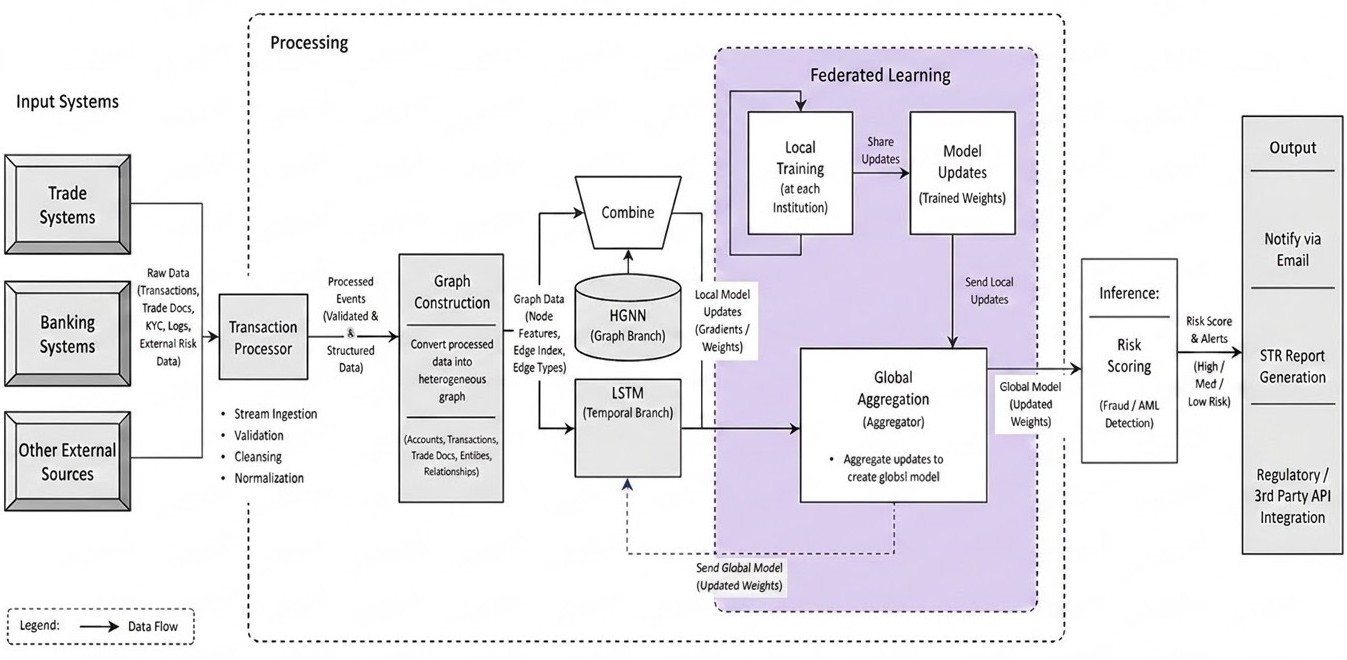
\includegraphics[width=0.98\textwidth]{Figures/overall_architecture.jpg}
    }
    \caption{Overall Architecture of the Proposed TBML Detection Framework}
    \label{fig:overall_architecture}
\end{figure}

%========================================================
\subsection[Data Flow Diagrams]{\textbf{Data Flow Diagrams}}
%========================================================

A Data Flow Diagram (DFD) is a simple way to show how data moves through a system and how processes, external entities, and data repositories relate to one another. DFDs make it easier to see how information enters the system, gets processed, is stored, and then moves to other components. In the proposed Federated Heterogeneous Graph Neural Network (HGNN)-Based Trade-Based Money Laundering (TBML) Detection System, they are used to represent transaction acquisition, graph construction, federated learning, fraud analysis, and alert generation. The split into Level 0, Level 1, and Level 2 diagrams gives a clearer view of the operational flow, the subsystem interactions, and the data-processing steps involved in real-time AML analytics. The diagrams follow the Yourdon and De Marco DFD methodology for consistency.

%========================================================
\subsubsection[Data Flow Diagram Level 0]{\textbf{Data Flow Diagram Level 0}}
%========================================================

\begin{figure}[H]
    \centering
    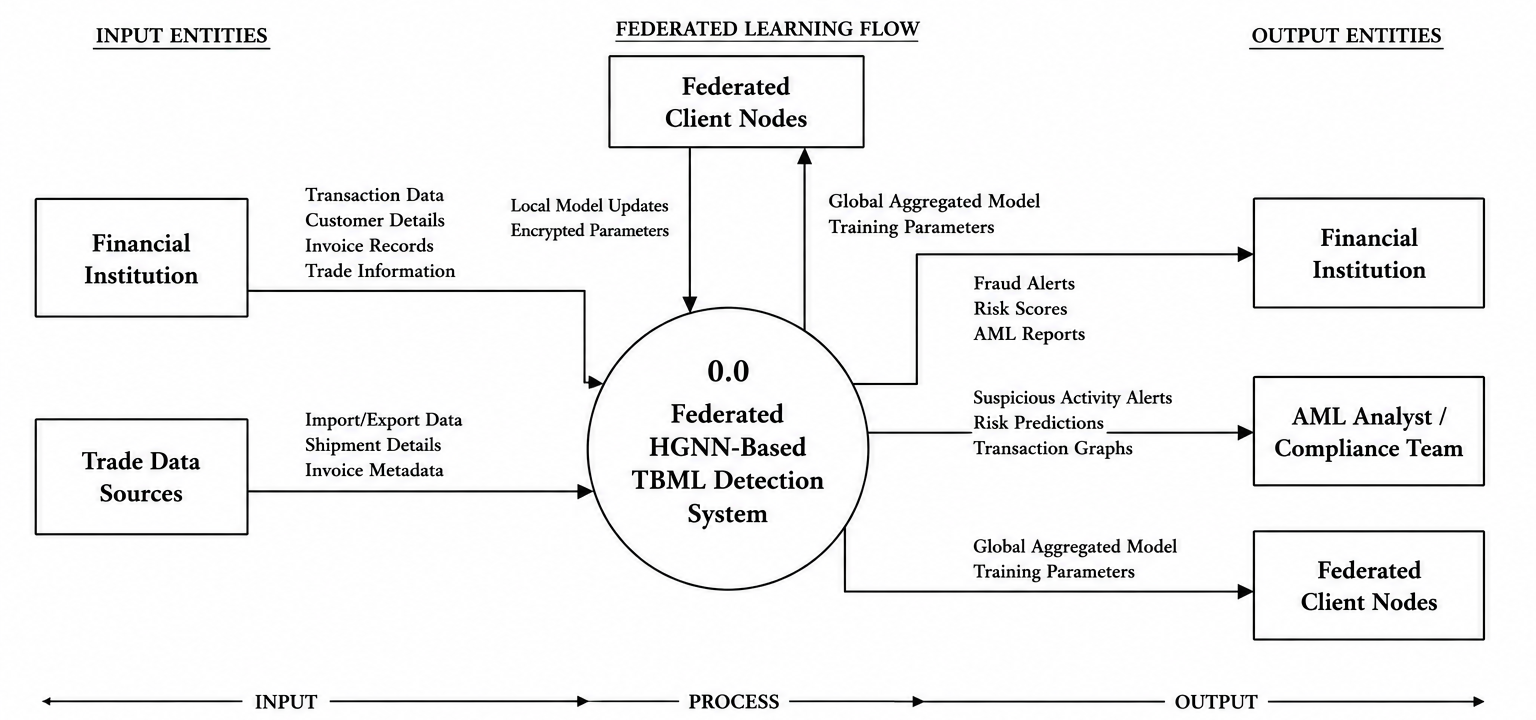
\includegraphics[width=0.95\linewidth]{Figures/DFD_Level_0.png}
    \caption{Level 0 Data Flow Diagram}
    \label{fig:dfd_level0}
\end{figure}

The Level 0 Data Flow Diagram (DFD) of the designed Federated HGNN-Based TBML Detection System is shown in Figure \ref{fig:dfd_level0}. It gives a top-level view of the system as a single process interacting with external entities such as Financial Institutions, Federated Client Nodes, AML Analysts, and Trade Data Sources. The system receives transaction records, customer information, invoice details, and trade details from financial institutions, while trade data sources contribute import/export records and shipment data that help validate transactions and support graph construction. Federated client nodes exchange encrypted local model parameters with the global model, and the system produces fraud warnings, risk assessments, AML reports, and suspicious activity notifications for analysts and compliance teams.

%========================================================
\subsubsection[Data Flow Diagram Level 1]{\textbf{Data Flow Diagram Level 1}}
%========================================================

\begin{figure}[H]
    \centering
    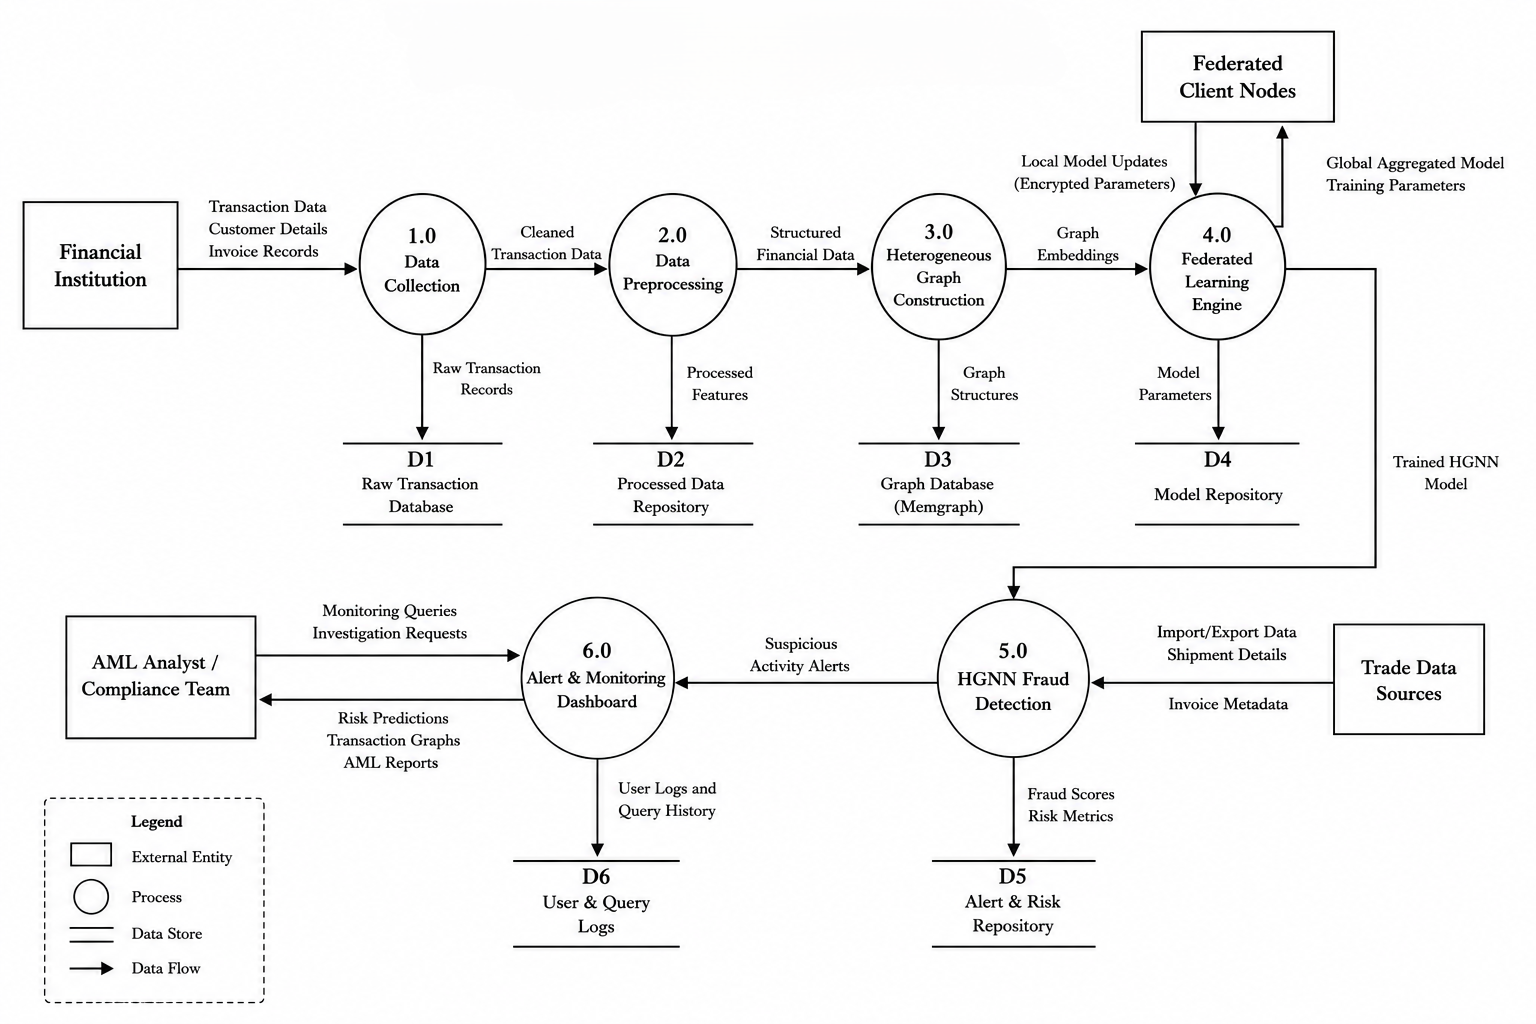
\includegraphics[width=\linewidth]{Figures/DFD_Level_1.png}
    \caption{Level 1 Data Flow Diagram}
    \label{fig:dfd_level1}
\end{figure}

The Level 1 Data Flow Diagram of the proposed TBML detection framework is shown in Figure \ref{fig:dfd_level1}. It breaks the main system into functional processes such as Data Collection, Data Preprocessing, Heterogeneous Graph Construction, Federated Learning Engine, HGNN Fraud Detection, and the Alert and Monitoring Dashboard. The Data Collection module gathers raw transactional data and customer data from financial institutions. That data is cleaned and transformed during preprocessing to produce structured financial features. Those features are then used by the graph construction engine to build heterogeneous graph representations stored in the graph database. The federated learning engine trains distributed collaborative models using encrypted local updates from federated client nodes while preserving institutional data privacy. The trained HGNN model is used by the fraud detection engine to identify suspicious transactional patterns, compute fraud scores, and generate anomaly alerts. Finally, the monitoring dashboard allows AML analysts and compliance teams to investigate cases, visualize transaction graphs, and review risk assessment reports in real time.
%========================================================
\subsubsection[Data Flow Diagram Level 2]{\textbf{Data Flow Diagram Level 2}}
%========================================================

\begin{figure}[H]
    \centering
    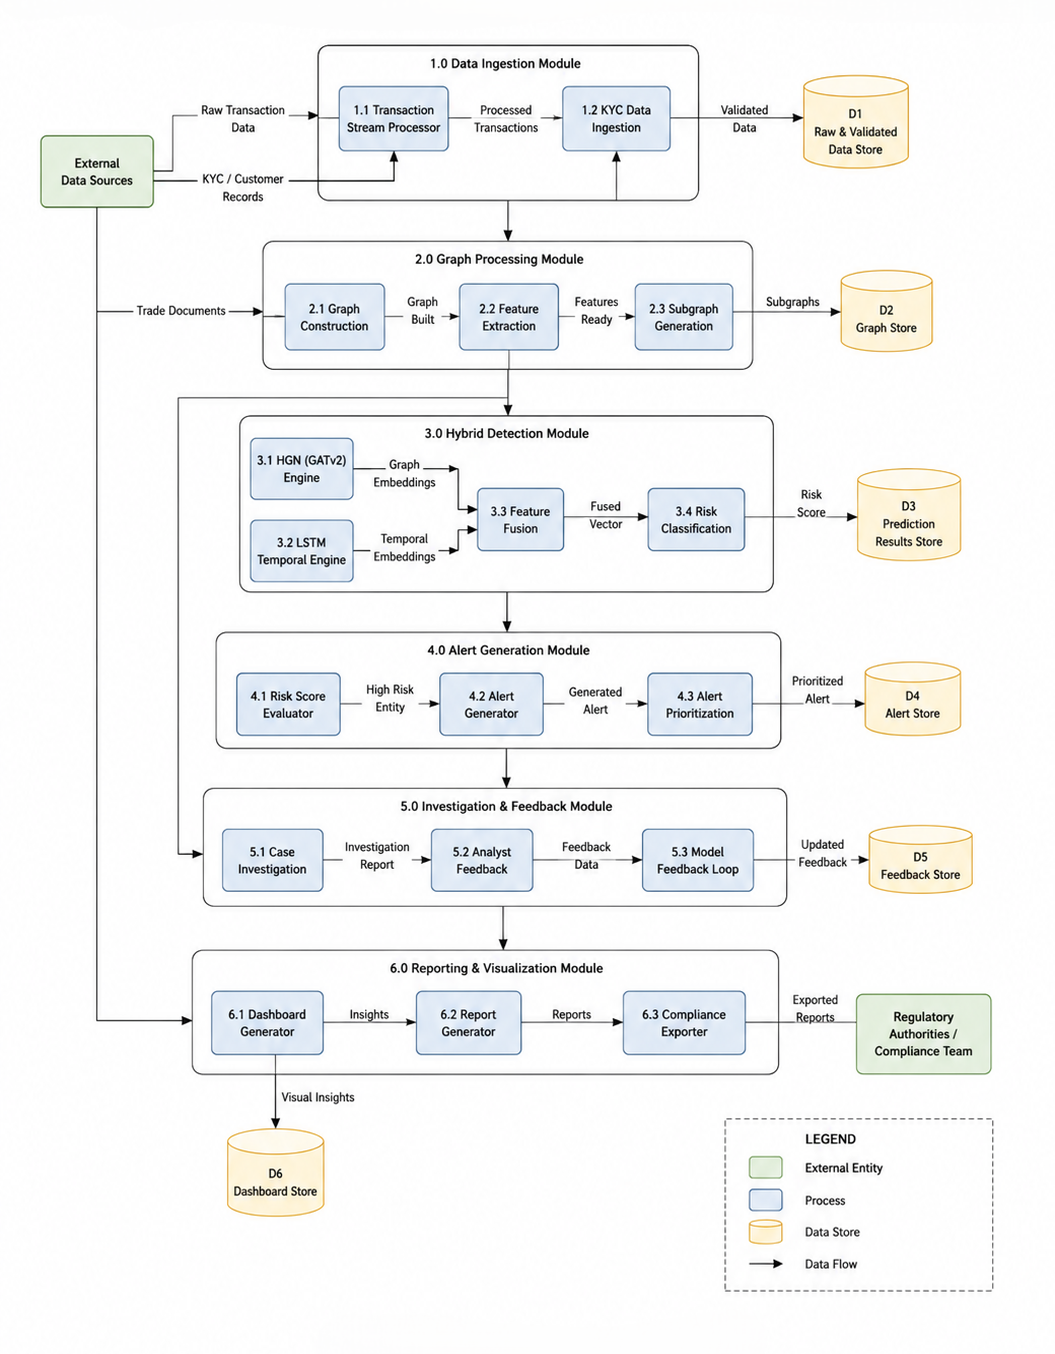
\includegraphics[width=\linewidth]{Figures/DFD_Level_2.png}
    \caption{Level 2 Data Flow Diagram}
    \label{fig:dfd_level2}
\end{figure}

Figure \ref{fig:dfd_level2} shows the Level 2 DFD, which breaks down the HGNN Fraud Detection module in more detail. The process begins with Data Integration and Validation, where trade invoice data, shipment data, and transactional metadata are checked for inconsistencies. After validation, the data moves into Entity Resolution and Feature Extraction, which handles attribute extraction and prepares the features needed for graph-based learning. Heterogeneous Graph Generation then builds the financial transaction graphs that connect entities, account relations, invoice transactions, and other trade-related structures. HGNN Inference and Risk Scoring applies the graph neural network to generate scores and identify suspicious transactional behavior. The results then move through Anomaly Detection and Classification, followed by Alert Generation and Prioritization, which ranks suspicious transactions according to risk. The final stage, Result Aggregation and Reporting, produces fraud summaries, alert notifications, and reports that are sent to the Alert and Monitoring Dashboard for review.


\section {Detailed System Design}
This section gives a detailed view of the system design for the proposed TBML detection framework. It covers the structure chart showing how the system components are organized, the functional descriptions of the major modules, and the interaction workflow between the services and analytical components in the framework.
%========================================================
\subsection[Structure Chart]{\textbf{Structure Chart}}
%========================================================
The structure chart of the proposed TBML detection framework shows how the key functional modules are arranged. The framework includes frontend, backend, fraud detection, federated learning, database, and compliance layers, all of which support scalable monitoring and intelligent fraud analysis in Anti-Money Laundering ecosystems.

The frontend layer provides dashboard interfaces, transaction monitoring, risk visualization, and STR management. The backend layer coordinates transactions between the frontend interface and the analytical modules by handling APIs, transaction management, authentication, and authorization. The fraud detection layer contains the Hybrid HGNN-LSTM modules that handle graph analytics, transaction analysis, feature fusion, and risk prediction.

The federated learning layer supports collaborative privacy-preserving model training and global model synchronization among participants. The database layer manages transactions, graphs, audit logs, and compliance data. The compliance layer handles STR generation, regulatory reporting, email notifications, and monitoring processes. The structural organization of the proposed TBML detection framework is shown in Figure~\ref{fig:structure_chart}.
\begin{figure}[H]
    \centering
    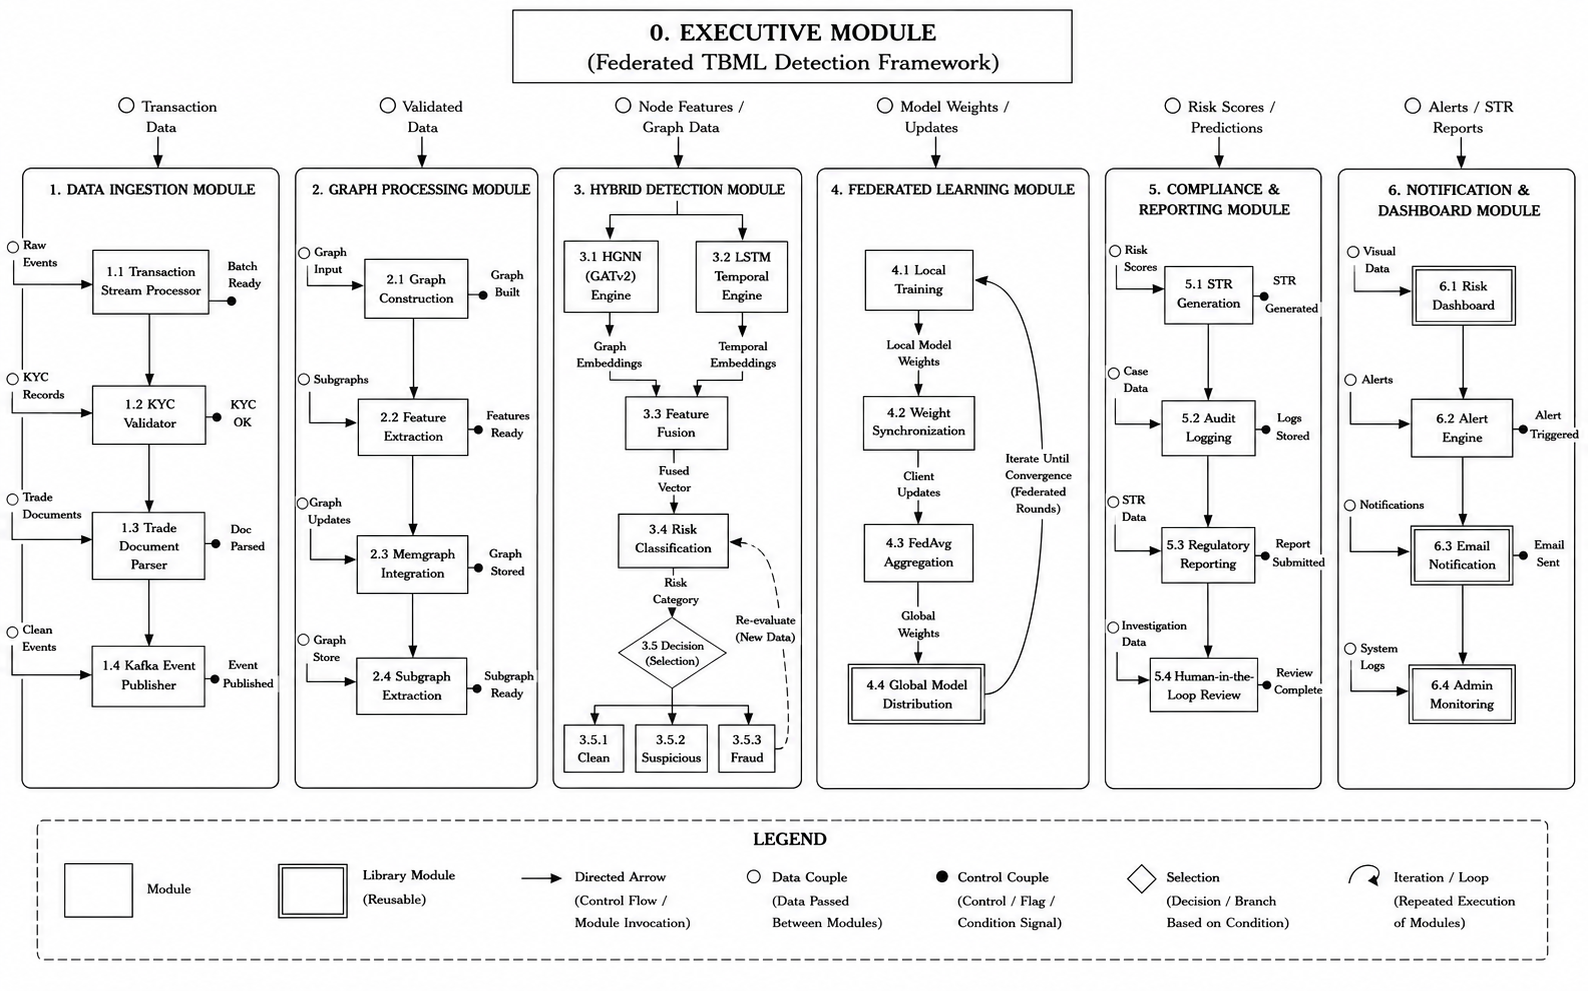
\includegraphics[width=\textwidth]{Figures/tbml_academic_structure_chart.png}
    \caption{Structure Chart of the Proposed TBML Detection Framework}
    \label{fig:structure_chart}
\end{figure}

The structure chart makes the modular organization of the framework easier to understand, especially the interaction between the analytical, monitoring, storage, and compliance-oriented services. This modular design improves scalability, maintainability, service integration, and coordination between the frontend interfaces, backend analytical services, and distributed fraud detection environments.

%========================================================
\subsection[Functional Description of the Modules]{\textbf{Functional Description of the Modules}}
%========================================================

The functional description of the modules explains the internal processing workflow and interaction between the major analytical, monitoring, and compliance-oriented components operating within the proposed TBML detection framework. The framework integrates transaction streaming services, graph construction mechanisms, hybrid HGNN--LSTM analytical models, institutional verification environments, and regulatory reporting systems to support intelligent Trade-Based Money Laundering detection and real-time compliance monitoring.

% %========================================================
% \subsection[Module Interaction Workflow]{\textbf{Module Interaction Workflow}}
% %========================================================

% The module interaction workflow shows how the main services of the proposed framework fit together, starting with transaction intake and ending with regulatory reporting. Financial transactions, KYC records, and trade documents first enter the transaction processing layer, where they are prepared and published to Kafka streaming topics for asynchronous communication between backend services.

% Kafka consumers read these transaction streams and pass the processed data to the graph construction and feature extraction module. Here, heterogeneous financial transaction graphs are built from accounts, transactions, trade entities, and document relationships stored in the Memgraph database. The resulting graph embeddings and relational features are then sent to the Hybrid HGNN--LSTM fraud detection module for graph representation learning, temporal transaction analysis, and fraud prediction.

% The fraud classifications and monitoring results produced by the analytical engine are stored in PostgreSQL and displayed in the dashboard environment for institutional investigators and banking administrators. Suspicious transactions are reviewed by authorized bank administrators and then marked as clean, suspicious, or confirmed fraudulent.

% Transactions confirmed as fraudulent are forwarded to the STR generation environment, where Suspicious Transaction Reports are prepared with support from the Groq API service. These reports are then reviewed by regulatory authorities responsible for investigation, inquiry, and enforcement. At the same time, notification management services coordinate fraud alerts and institutional communication, while the Resend email service delivers notification emails and regulatory messages to the relevant authorities. The overall module interaction workflow of the proposed TBML detection framework is illustrated in Figure~\ref{fig:workflow_interaction}.

\begin{figure}[H]
    \centering
    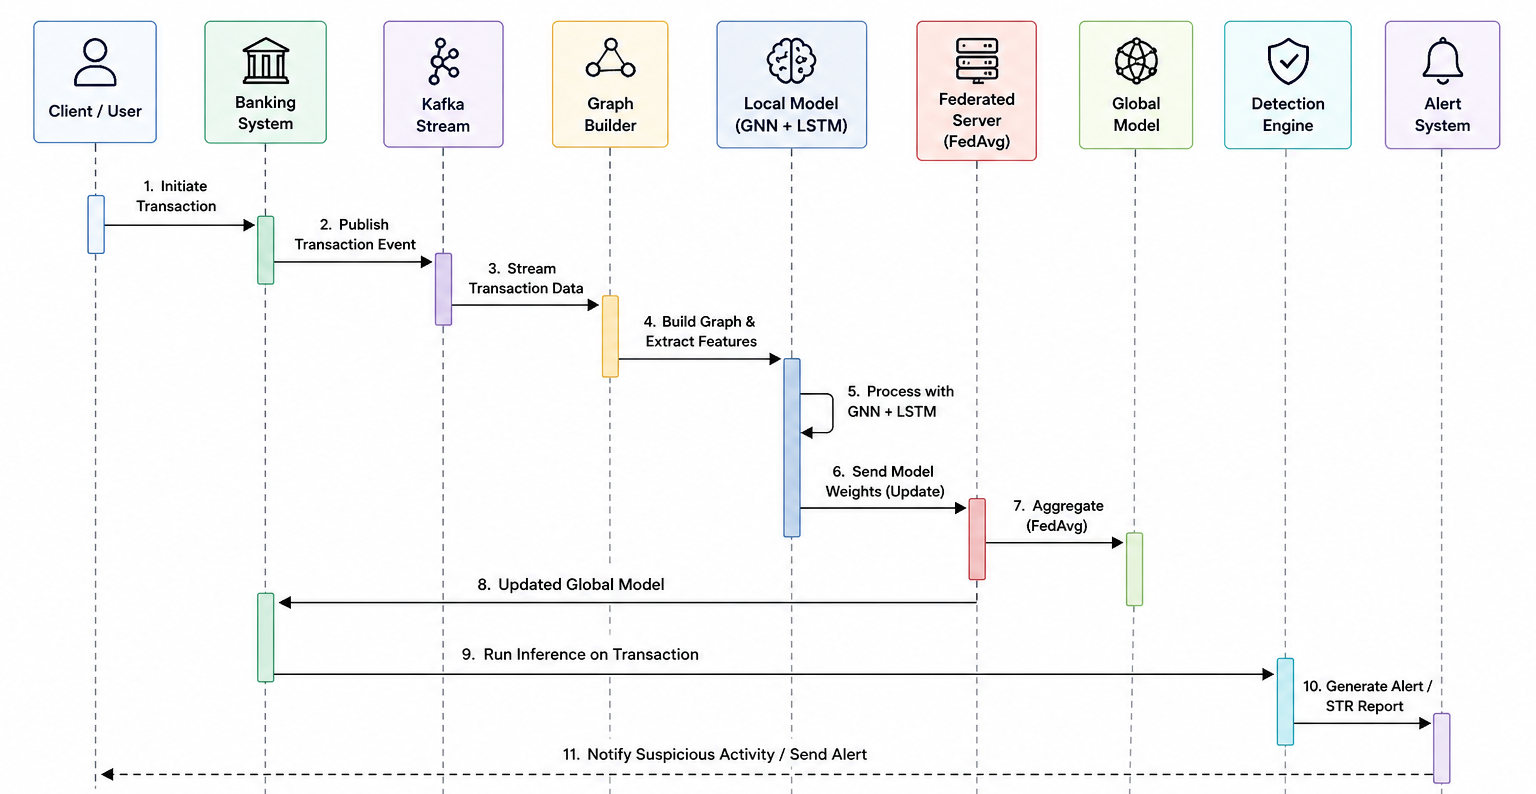
\includegraphics[width=\textwidth]{Figures/sequencediagramfinal.png}
    \caption{Workflow Interaction Diagram for the Proposed TBML Detection Framework}
    \label{fig:workflow_interaction}
\end{figure}

The workflow interaction diagram shows the coordinated interaction between streaming services, graph-based analytical modules, monitoring environments, institutional verification systems, and regulatory compliance services operating within the proposed framework. This modular workflow supports scalable transaction processing, intelligent fraud analysis, compliance management, and real-time Anti-Money Laundering monitoring across distributed financial environments.

%========================================================
\subsubsection[Transaction Processing Module]{\textbf{Transaction Processing Module}}
%========================================================

The transaction processing Module acts as the initial ingestion environment within the proposed TBML detection framework. This Module collects financial transactions, KYC records, trade documents, and institutional monitoring events originating from banking systems and external financial environments.

The input data processed within this Module includes sender and receiver account identifiers, transaction amounts, commodity types, trade quantities, trade values, invoice details, transaction timestamps, and institutional monitoring attributes associated with financial activities. The collected transactional data is validated, normalized, and converted into structured transaction records to support reliable downstream analytical processing.

The processed transaction events are published into Kafka streaming topics to enable asynchronous communication between backend services and analytical modules. The generated transaction streams serve as the primary input for graph construction, feature extraction, and graph-based fraud detection operations within the proposed framework.
%========================================================
\subsubsection[Graph Construction Module]{\textbf{Graph Construction Module}}
%========================================================

The graph construction module transforms processed transaction streams into heterogeneous financial transaction graphs for downstream graph-based analytical processing. The module receives validated transaction events from Kafka consumer services and models financial interactions between accounts, transactions, and trade documents within a connected graph environment.

The generated graph schema consists of interconnected node entities including \texttt{(:Account)}, \texttt{(:Transaction)}, and \texttt{(:Document)} connected through relationships such as \texttt{[:SENDS]}, \texttt{[:TO]}, and \texttt{[:HAS\_DOC]} as illustrated in Figure~\ref{fig:graph_schema}. The heterogeneous graph structure preserves transactional connectivity, intermediary account interactions, and trade-document relationships required for identifying hidden financial dependencies associated with Trade-Based Money Laundering activities.

The module interacts with the Memgraph database to store graph structures, entity relationships, and transactional connectivity information required for downstream feature extraction and fraud analysis. The generated graph representations and extracted relational features are subsequently forwarded to the Hybrid HGNN--LSTM fraud detection module for intelligent transaction classification.

\begin{figure}[H]
\centering

\begin{tikzpicture}[
    node distance=3cm,
    every node/.style={font=\scriptsize},
    entity/.style={
        draw=black,
        thick,
        rounded corners=8pt,
        align=center,
        minimum width=3cm,
        minimum height=2.2cm
    },
    relation/.style={
        -{Latex[length=2.5mm]},
        thick
    }
]

% ==========================================================
% ACCOUNT NODE
% ==========================================================

\node[
    entity,
    fill=orange!25
] (account)
{
\textbf{(:Account)}\\
\rule{2.2cm}{0.3pt}\\
account\_id\\
jurisdiction\\
is\_shell\\
dorm\_days
};

% ==========================================================
% TRANSACTION NODE
% ==========================================================

\node[
    entity,
    fill=red!20,
    right=of account
] (transaction)
{
\textbf{(:Transaction)}\\
\rule{2.2cm}{0.3pt}\\
txn\_id\\
amount\\
timestamp\\
risk\_score
};

% ==========================================================
% DOCUMENT NODE
% ==========================================================

\node[
    entity,
    fill=yellow!30,
    above=of transaction
] (document)
{
\textbf{(:Document)}\\
\rule{2.2cm}{0.3pt}\\
swift\_ref\\
price\_deviation\\
weight\_gap\\
commodity
};

% ==========================================================
% RELATIONSHIPS
% ==========================================================

\draw[relation]
(account) to[bend left=18]
node[midway, above] {\texttt{[:SENDS]}}
(transaction);

\draw[relation]
(transaction) to[bend left=18]
node[midway, below] {\texttt{[:TO]}}
(account);

\draw[relation]
(transaction) --
node[midway, right] {\texttt{[:HAS\_DOC]}}
(document);

\end{tikzpicture}

\caption{Heterogeneous graph schema representing entity attributes and transactional relationships in the proposed TBML detection framework.}

\label{fig:graph_schema}

\end{figure}


%========================================================
\subsubsection[Hybrid HGNN--LSTM Fraud Detection Module]{\textbf{Hybrid HGNN--LSTM Fraud Detection Module}}
%========================================================
The Hybrid HGNN--LSTM fraud detection module performs graph-based representation learning and temporal transaction analysis within the proposed TBML detection framework. The module receives KYC node features, graph edge relationships, SWIFT transaction attributes, sequential transaction tensors, and trade metadata extracted from the heterogeneous financial graph for downstream analytical processing.

The graph branch utilizes a three-layer GATv2 architecture to perform attention-based neighborhood aggregation and multi-hop message passing across interconnected financial entities. The stacked GATv2 layers improve two-hop neighborhood visibility and enable the model to capture hidden transactional relationships and intermediary account interactions associated with Trade-Based Money Laundering activities. The generated graph embeddings are globally pooled and fused with sequential transaction representations before being processed through the LSTM branch for temporal anomaly detection and transaction behavior analysis. In parallel, the trade branch processes trade-specific attributes including price deviation and weight gap scores using multilayer perceptron operations and feature normalization layers.

\begin{figure}[H]
    \centering
    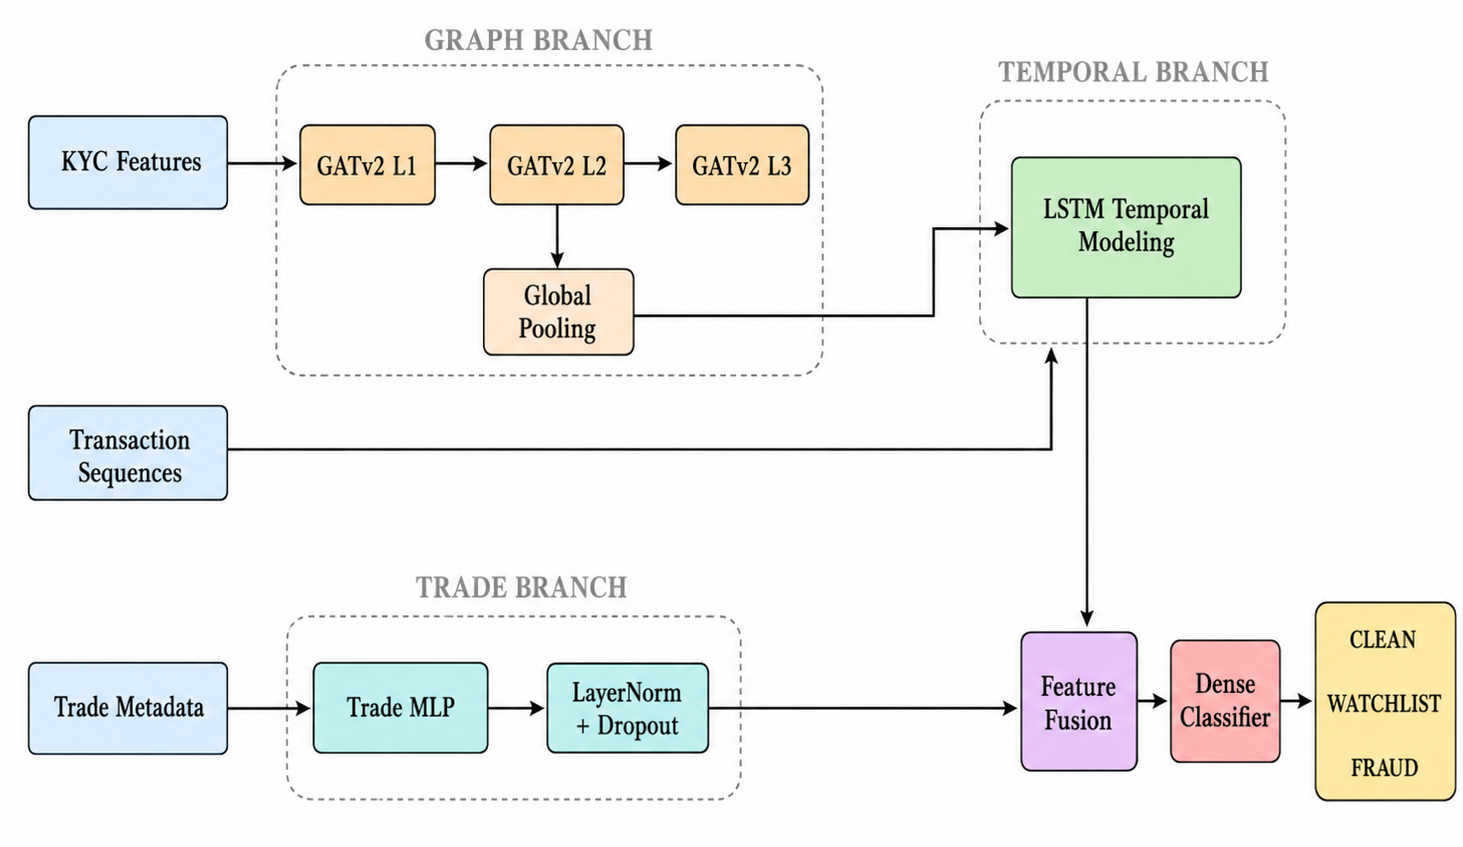
\includegraphics[width=\textwidth]{Figures/aimodel.png}
    \caption{Architecture of the Proposed Hybrid HGNN--LSTM Fraud Detection Module}
    \label{fig:hgnn_architecture}
\end{figure}

The generated graph embeddings, temporal representations, and trade feature vectors are combined within the feature fusion layer for downstream fraud prediction and transaction risk analysis. The final dense classification layer categorizes transactions into predefined classes including \texttt{CLEAN}, \texttt{WATCHLIST}, and \texttt{FRAUD}. The overall architecture of the proposed Hybrid HGNN--LSTM fraud detection module is illustrated in Figure~\ref{fig:hgnn_architecture}.

%========================================================
\subsubsection[Federated Learning Module]{\textbf{Federated Learning Module}}
%========================================================
The federated learning module enables privacy-preserving collaborative fraud detection across distributed financial institutions without directly sharing sensitive transactional data. Each participating institution performs local model training using institutional transaction graphs, transaction sequences, and fraud classification labels generated within the analytical environment. Independent federated clients maintain isolated training environments and perform localized optimization of the Hybrid HGNN--LSTM model on institution-specific financial datasets.

\begin{figure}[H]
    \centering
    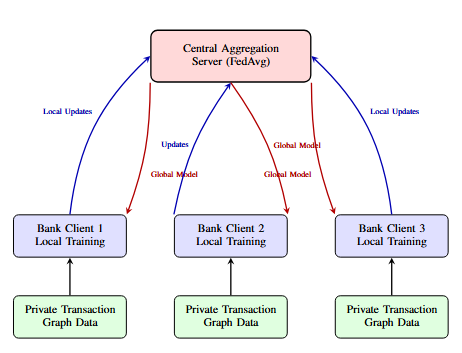
\includegraphics[width=0.82\textwidth]{Figures/federated_architecture.png}
    \caption{Federated learning architecture for privacy-preserving collaborative TBML detection across distributed institutions}
    \label{fig:federated_architecture}
\end{figure}

The framework utilizes the Federated Averaging (\texttt{FedAvg}) strategy to aggregate distributed model parameters across participating institutions. During each federated communication round, locally trained model weights generated from individual institutional clients are transmitted to the central aggregation server where parameter averaging operations are performed to generate a globally optimized fraud detection model. The aggregated global model parameters are subsequently redistributed to participating institutions for synchronized fraud detection and continuous real-time analytical inference. The overall federated learning architecture of the proposed framework is illustrated in Figure~\ref{fig:federated_architecture}.

%========================================================
\subsubsection[STR Generation and Notification Module]{\textbf{STR Generation and Notification Module}}
%========================================================

The STR generation and notification module is responsible for compliance reporting and fraud alert management within the proposed TBML detection framework. Transactions verified as fraudulent by authorized banking administrators are forwarded to this module for Suspicious Transaction Report (STR) generation and regulatory processing. The module generates STR reports containing transaction details, fraud classifications, trade metadata, institutional information, and investigation summaries associated with suspicious financial activities.

The Groq API service is utilized for analytical summarization and automated assistance during compliance documentation generation. Generated STR reports are subsequently forwarded to regulatory monitoring authorities for investigation and enforcement procedures. The notification management environment coordinates fraud alerts and institutional communication workflows, while the Resend email service delivers notification emails, investigation alerts, and regulatory enforcement messages to banking institutions and regulatory authorities.

%========================================================
\subsubsection[Dashboard and Regulatory Monitoring Module]{\textbf{Dashboard and Regulatory Monitoring Module}}
%========================================================

The dashboard and regulatory monitoring module provides real-time transaction visualization, fraud monitoring, and institutional investigation functionalities within the proposed TBML detection framework. The monitoring dashboard displays transaction classifications, fraud alerts, risk scores, STR records, and analytical monitoring information generated by the fraud detection environment. Separate dashboard environments are maintained for banking administrators and regulatory authorities to support institution-level monitoring and centralized compliance management operations.

For banking administrators, the dashboard provides a clear view of suspicious and fraudulent transactions flagged by the analytical model. They can review each case, verify the context, and then classify it as \texttt{CLEAN}, \texttt{WATCHLIST}, or \texttt{FRAUD}. This review step helps reduce false alarms while ensuring that genuine suspicious activity is escalated for further action. Transactions confirmed as fraudulent are then passed on for Suspicious Transaction Report (STR) generation and regulatory reporting.

Regulatory authorities use a separate monitoring view to track generated STR reports and institution-level fraud cases in one place. From this interface, they can follow compliance activity, request supporting documents, initiate inquiry procedures, and carry out account freeze operations when necessary. The overall workflow is illustrated in Figure~\ref{fig:realtime_workflow_final}.

\begin{figure}[H]
\centering
\resizebox{0.98\columnwidth}{!}{
\begin{tikzpicture}[
    node distance=1.1cm and 1.1cm,
    >=stealth,
    thick,
    every node/.style={font=\scriptsize},
    block/.style={
        draw,
        rectangle,
        rounded corners=3pt,
        align=center,
        minimum width=2.4cm,
        minimum height=0.9cm
    },
    storage/.style={
        draw,
        cylinder,
        shape border rotate=90,
        aspect=0.3,
        align=center,
        minimum height=1cm,
        minimum width=1.2cm
    }
]

\node[block, fill=blue!12] (txn) {Incoming\\Transactions};
\node[block, fill=orange!15, right=of txn] (kafka) {Kafka Streaming\\\& Graph Update};
\node[block, fill=green!15, right=of kafka] (model) {HGNN-LSTM\\Inference Model};
\node[block, fill=yellow!18, right=of model] (risk) {\texttt{CLEAN}\\ \texttt{WATCHLIST}\\ \texttt{FRAUD}};

\node[block, fill=cyan!15, below=1.8cm of model] (bank) {BankUser\\Dashboard};
\node[block, fill=red!15, left=of bank] (str) {STR Generation\\(GROQ LLaMA-70B)};
\node[block, fill=purple!15, right=of bank] (notify) {Email / Push\\Notification};

\node[block, fill=pink!18, below=1.8cm of notify] (admin) {Admin\\Dashboard};
\node[block, fill=orange!18, left=of admin] (action) {Freeze Account /\\Request Documents};

\node[storage, fill=gray!15] (db) at ($(action.west)-(2.2,0)$) {PostgreSQL};

\draw[->] (txn) -- (kafka);
\draw[->] (kafka) -- (model);
\draw[->] (model) -- (risk);

\draw[->] (risk.south) -- ++(0,-0.5) -| (bank.north);

\draw[->] (bank) -- (str);
\draw[->] (str.north) -- ++(0,0.4) -| (notify.north);
\draw[->] (notify) -- (admin);
\draw[->] (admin) -- (action);

\draw[->, dashed] (action.west) -- (db.east);
\draw[->, dashed] (str.south) |- (db.north);
\draw[<->, dashed] (bank.south) -- ++(0,-0.6) -| (db.north);
\draw[<->, dashed] (admin.south) |- ++(0,-0.5) -| (db.south);

\end{tikzpicture}
}
\caption{Real-time fraud inference and compliance workflow of the proposed TBML detection framework.}
\label{fig:realtime_workflow_final}
\end{figure}

%========================================================
\section[Summary]{\textbf{Summary}}
%========================================================

This chapter provided a detailed overview of the software specifications, architectural design, data flow diagrams, structure chart, and functional descriptions of the major modules in the proposed TBML detection framework. The discussion of the system architecture, module interactions, and analytical workflows gives a clearer picture of the operational mechanisms, service integration strategy, and real-time monitoring capabilities built into the framework for intelligent Trade-Based Money Laundering detection and compliance management across distributed financial environments.



		
		%Chapter 4
		%========================================================
\chapter{High Level Design}
%========================================================

This Chapter presents the high level design of the proposed TBML detection framework including architectural approaches, design aspects related to the software and the
entire system architecture combining the capabilities of graph-based fraud detection, federated learning, and real-time transaction monitoring in the unified compliance solution.

%========================================================
\section[Design Considerations]{\textbf{Design Considerations}}
%========================================================

A number of operational, analytical and security-related factors affect the design of the
proposed TBML detection framework due to the nature of Trade-Based Money
Laundering which includes complex interconnections between different financial
organizations and their transactions. Therefore, the architecture of the proposed
solution has to address the requirements for large-scale analytical processing and
secure collaboration between the institutions, as well as the ability to efficiently perform
graph-based fraud analysis. The key design considerations of the proposed
framework are discussed in the following subsections.

%========================================================
\subsection[General Considerations]{\textbf{General Considerations}}
%========================================================
The proposed TBML detection framework is designed to analyze large transaction volumes from multiple financial organizations. Since laundering schemes always include
interconnected accounts, trade companies, invoices, and other relationships, the framework employs graph-based modeling approaches that allow for better representation of the hidden financial dependencies compared to traditional relational models.
Additionally, the architecture of the proposed framework allows for real-time
transaction processing.

Security, privacy protection, and the scalability of the system have to be considered as critical aspects of the proposed architecture since financial and compliance-related data will need to be handled. In order to fulfill the stated requirements, the framework will include secure authentication techniques, role-based access controls, and federated learning approaches for protected cooperation across organizations without exposing transactional information. System design is based on the use of modular architecture to facilitate easier implementation, maintenance, and future enhancements to transaction monitoring, fraud detection, compliance reporting, and dashboards visualization services

%========================================================
\subsection[Development Methods]{\textbf{Development Methods}}
%========================================================
The proposed TBML detection framework is designed in a modular and iterative style of development to enable scalable system integration for future continuous development and improvement of analytical functionalities. Individual system components, such as transaction monitoring services, graph construction pipelines, fraud detection models, federated learning environments, and dashboard interfaces are built and tested separately from the rest of the system and then incorporated into the full monitoring system.

The development process also involves iterative modelling evaluation and experimentation, which will enhance fraud detection performance and analytical reliability. Processed transactional data are used for training graph-based machine learning models, while the use of API-based communication mechanisms enables the integration of frontend and backend services to enable real-time interaction between the monitoring modules and the analytical services.

From the beginning of implementation, version control and collaborative development practices are used to manage the backend services, machine learning workflows, front-end interfaces, and analytical configurations in an efficient way. This is the modular development approach, which will facilitate the debugging, testing, maintenance and further development of the proposed framework for fraud detection.
%========================================================
\section[Architectural Strategies]{\textbf{Architectural Strategies}}
%========================================================

The architectural approaches taken in the proposed TBML detection framework aim at providing scalable financial transaction analysis, secure collaboration between institutions, and efficient communication between analytical services and monitoring interfaces. All these components, including graph-based models, backend analytical services, real-time dashboards, and distributed learning mechanisms are combined into a single monitoring environment. Some major architectural schemes related to the proposed framework are discussed in the following subsections.

%========================================================
\subsection[Programming Language]{\textbf{Programming Language}}
%========================================================

The proposed TBML detection framework primarily utilizes Python for backend services, graph processing, machine learning workflows, and analytical computations. Python was selected due to its extensive support for deep learning libraries, graph analytical frameworks, and federated learning environments. Libraries such as PyTorch, PyTorch Geometric, and Flower are utilized for implementing graph neural network models and distributed learning mechanisms within the fraud detection framework.

The frontend monitoring dashboard is built with Next.js and React.js for responsive UI development and real-time analytical visualization. Implementing dashboard components, transaction monitoring interfaces and compliance management services are done in JavaScript and TypeScript. FastAPI is also built-in to enable communication between front-end dashboards, back-end services, and machine learning modules via APIs.

%========================================================
\subsection[System Integration Architecture]{\textbf{System Integration Architecture}}
%========================================================
The proposed TBML detection framework is mainly based on Python as a back-end, graph processing, machine learning pipeline and analytical computation language. The decision to use Python was made because of its support with deep learning libraries, graph analytical frameworks, and federated learning environments. In this framework, the fraud detection models and distributed learning mechanisms are implemented using libraries like PyTorch, PyTorch Geometric, and Flower, which are used for implementing graph neural network models and distributed learning mechanisms within the framework of fraud detection

%========================================================
\subsection[Data Storage Management]{\textbf{Data Storage Management}}
%========================================================

The proposed TBML detection framework utilizes both relational and graph-based database systems to support efficient financial data management and analytical processing. PostgreSQL is utilized for storing structured transactional records, authentication information, compliance-related data, and generated Suspicious Transaction Reports. The relational database environment supports secure storage and efficient retrieval of operational monitoring information within the framework.

Memgraph is utilized as the graph database environment for storing interconnected financial entities and transactional relationships. Accounts, organizations, invoices, and transactions are represented as graph nodes and edges to support relational fraud analysis and graph neural network processing. The combined relational and graph-based storage strategy improves scalability, analytical flexibility, and efficient synchronization between backend analytical services and monitoring dashboards.

%========================================================
\section[Overall System Architecture]{\textbf{Overall System Architecture}}
%========================================================
The proposed TBML detection framework is aimed at providing intelligence to enable
intelligent financial transaction monitoring, relational fraud analysis, federated learning, and compliance reporting on TBML cases. The system encompasses transaction processing,
construction of a heterogeneous graph, fraud detection through machine learning algorithms, and monitoring of suspicious TBML transactions.
The architecture starts from multiple data sources like bank systems,
trade systems, and external financial service providers. The transaction data, trade information,
KYC details, and monitoring activities are then captured and passed through a transaction
processing module responsible for performing data validation, cleaning, normalization,
and event creation. The cleaned data is then transformed into heterogeneous graph structures where the entities like accounts, organizations, invoices, and transactions are modeled in terms of interconnected nodes and edges. It helps in identifying the hidden financial relations and suspicious transactions needed for learning from graphs.
The fraud detection framework includes Hybrid Graph Neural Network for relation analysis and temporal learning for transactional analysis. Both of these techniques are helpful in capturing complex launderers' behavior and improving the accuracy of fraud detection based on risk predictions. For ensuring the privacy of the data, federated learning is employed in this architecture, where all institutions train their models locally but share only their model parameters with the global aggregation module.

The aggregated global model is used in the inference and risk scoring module to classify the transactions as suspicious transactions and produce the risk scores of fraud. High-risk transactions would be sent to the compliance management module in order to trigger alerts, Suspicious Transaction Report generation, and regulations support. The total architecture of the proposed TBML detection framework is shown in Figure 4.1.Figure 4.1: Overall Architecture of the Proposed TBML Detection Framework 4.4 Data Flow Diagrams

\begin{figure}[H]
    \centering
    \fbox{
        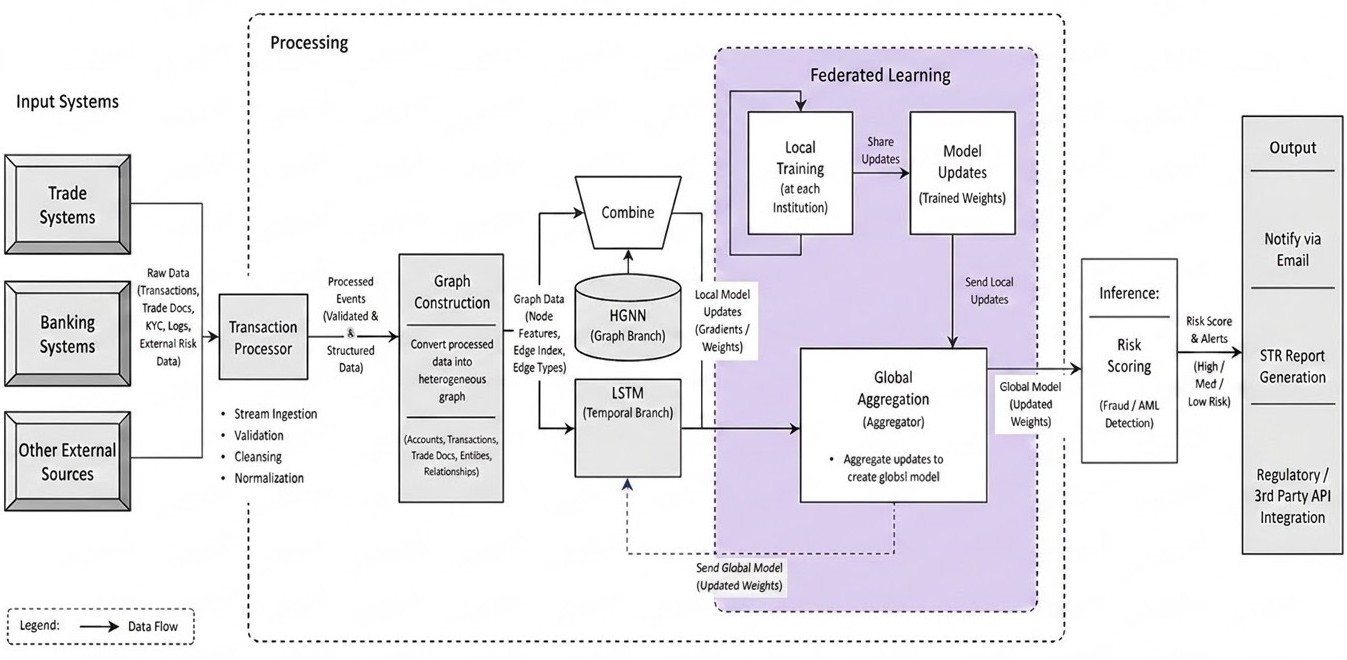
\includegraphics[width=0.98\textwidth]{Figures/overall_architecture.jpg}
    }
    \caption{Overall Architecture of the Proposed TBML Detection Framework}
    \label{fig:overall_architecture}
\end{figure}

%========================================================
\section[Data Flow Diagrams]{\textbf{Data Flow Diagrams}}
%========================================================

Data Flow Diagram (DFD) is the graphical tool used to present the movement of
data within a system and interactions among process, external entity, and data store.
DFDs are useful in illustrating the flow of information through system architecture in terms of data entry, data processing, data storage, and data transfer. Within the proposed Federated Heterogeneous Graph Neural Network (HGNN)-Based Trade-Based Money Laundering (TBML) Detection System, DFDs have been used to describe the entire workflow including transaction gathering, graph building, federated learning, fraud analysis, and alert generation. Decomposing the system architecture into Level 0, Level 1, and Level 2 diagrams helps gain a deeper insight about operation flow, subsystem interaction, and data processing.

%========================================================
\subsection[Data Flow Diagram Level 0]{\textbf{Data Flow Diagram Level 0}}
%========================================================

\begin{figure}[H]
    \centering
    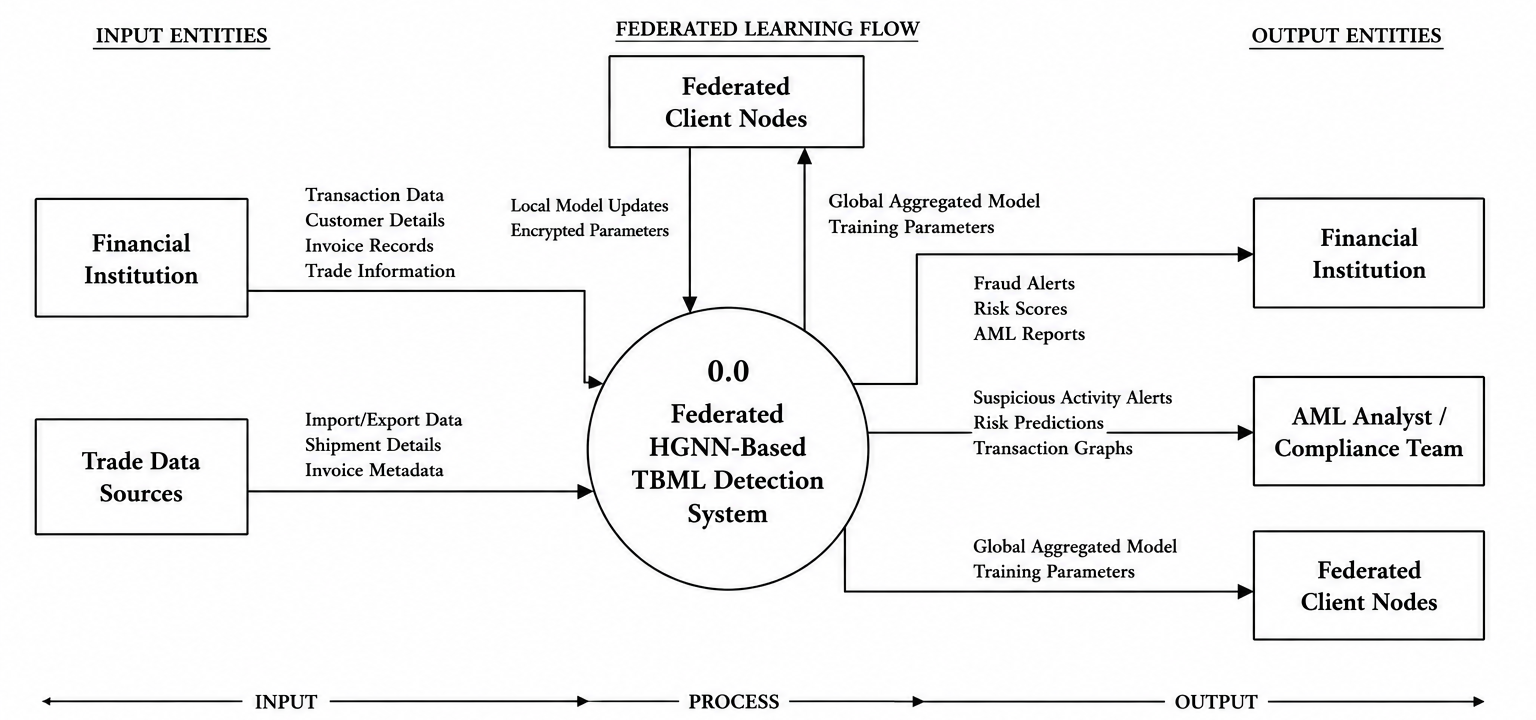
\includegraphics[width=0.95\linewidth]{Figures/DFD_Level_0.png}
    \caption{Level 0 Data Flow Diagram}
    \label{fig:dfd_level0}
\end{figure}

Figure \ref{fig:dfd_level0} shows the Level 0 Data Flow Diagram of the suggested Federated HGNN-Based TBML Detection System. This diagram serves as a high-level context-based representation of the entire system operating as one process involving various external participants such as Financial Institutions, Federated Client Nodes, AML Analysts, and Trade Data Sources. Financial Institutions supply transactions data, customers' data, invoice data, and other relevant data for processing by the system. Trade Data Sources offer the necessary import-export data and shipping information needed for transaction validation and graph creation. Federated Client Nodes share their locally trained model weights, which are then aggregated for global model training. Using these inputs, the system creates alerts, risks predictions, AML reports, and suspicious activities notifications that could be useful for compliance officers and financial analysts.
%========================================================
\subsection[Data Flow Diagram Level 1]{\textbf{Data Flow Diagram Level 1}}
%========================================================

\begin{figure}[H]
    \centering
    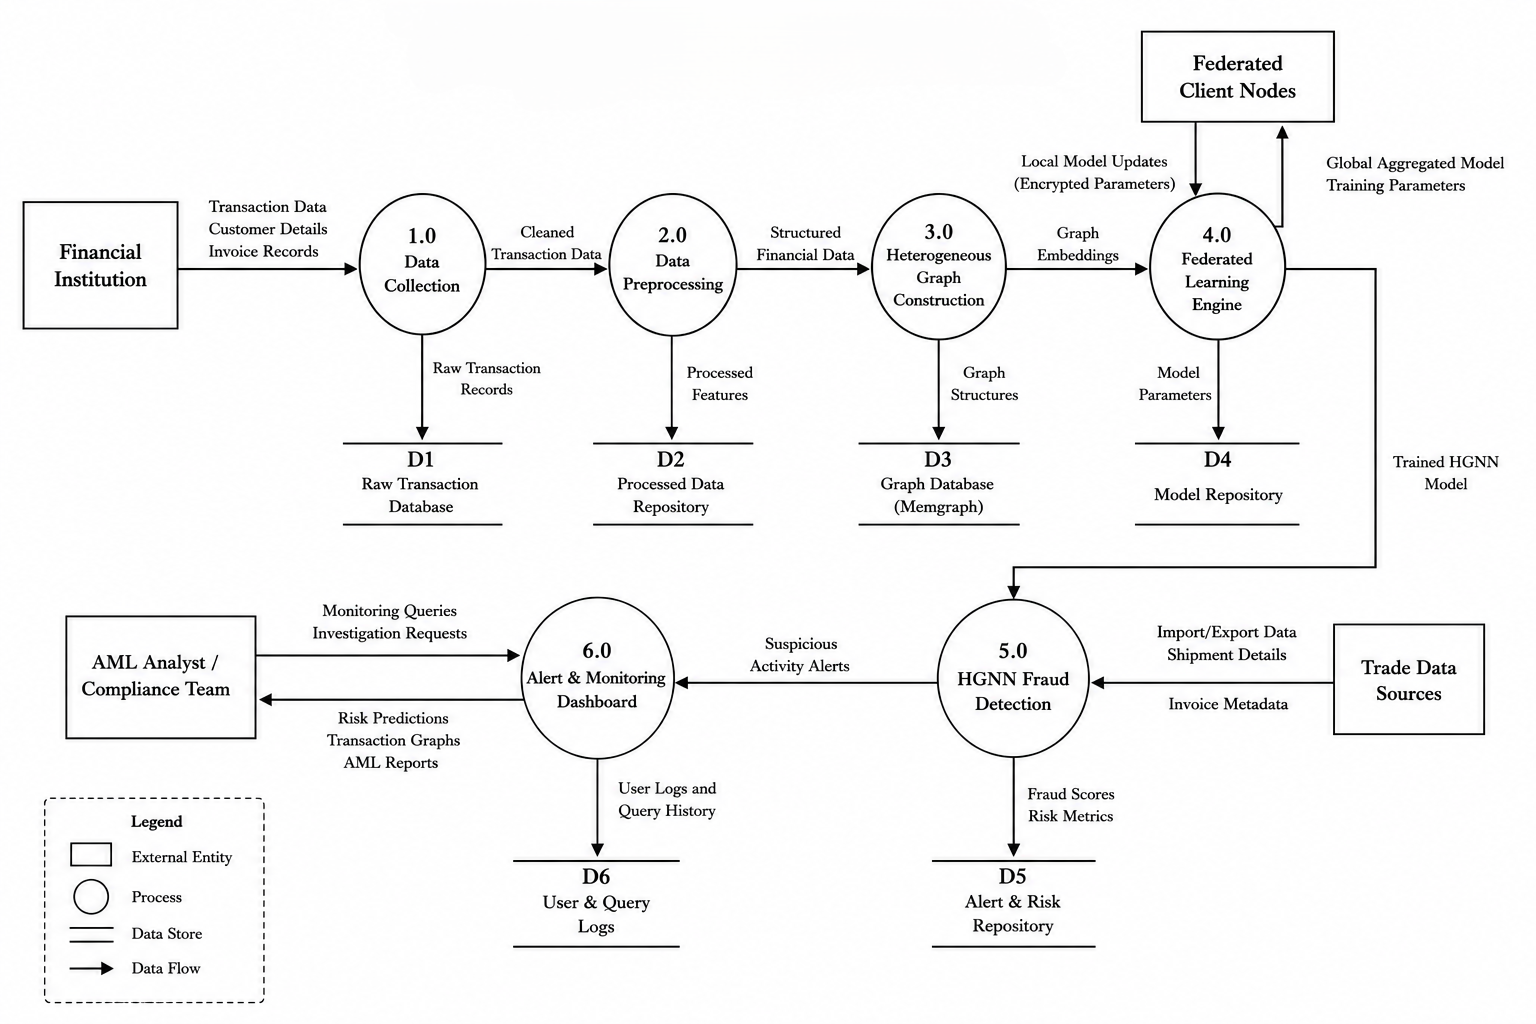
\includegraphics[width=\linewidth]{Figures/DFD_Level_1.png}
    \caption{Level 1 Data Flow Diagram}
    \label{fig:dfd_level1}
\end{figure}

Figure \ref{fig:dfd_level1} illustrates the level 1 data flow diagram of the designed TBML detection framework is illustrated through breaking down the main system architecture into several
processes. In particular, the architecture is made up of different modules including
Data Collection, Data Preprocessing, Heterogeneous Graph Construction,
Federated Learning Engine, HGNN Fraud Detection, and Alert and Monitoring
Dashboard. The Data Collection module is responsible for fetching raw transactional data and customer data from financial institutions; such data are cleaned and preprocessed to create structured financial features that can be used for building a heterogeneous
graph representation by graph construction engines in the graph database. As such,
the federated learning engine engages in conducting distributed collaborative model
training by using the encrypted local updates sent by federated clients without
violating the data privacy of institutions. The generated HGNN models are then used
by the fraud detection engine to detect any suspicious transaction, compute the fraud
scores, and raise alerts. Lastly, the investigation can be carried out by AML analysts
and compliance teams through the dashboard system.


%========================================================
\subsection[Data Flow Diagram Level 2]{\textbf{Data Flow Diagram Level 2}}
%========================================================
\begin{figure}[H]
    \centering
    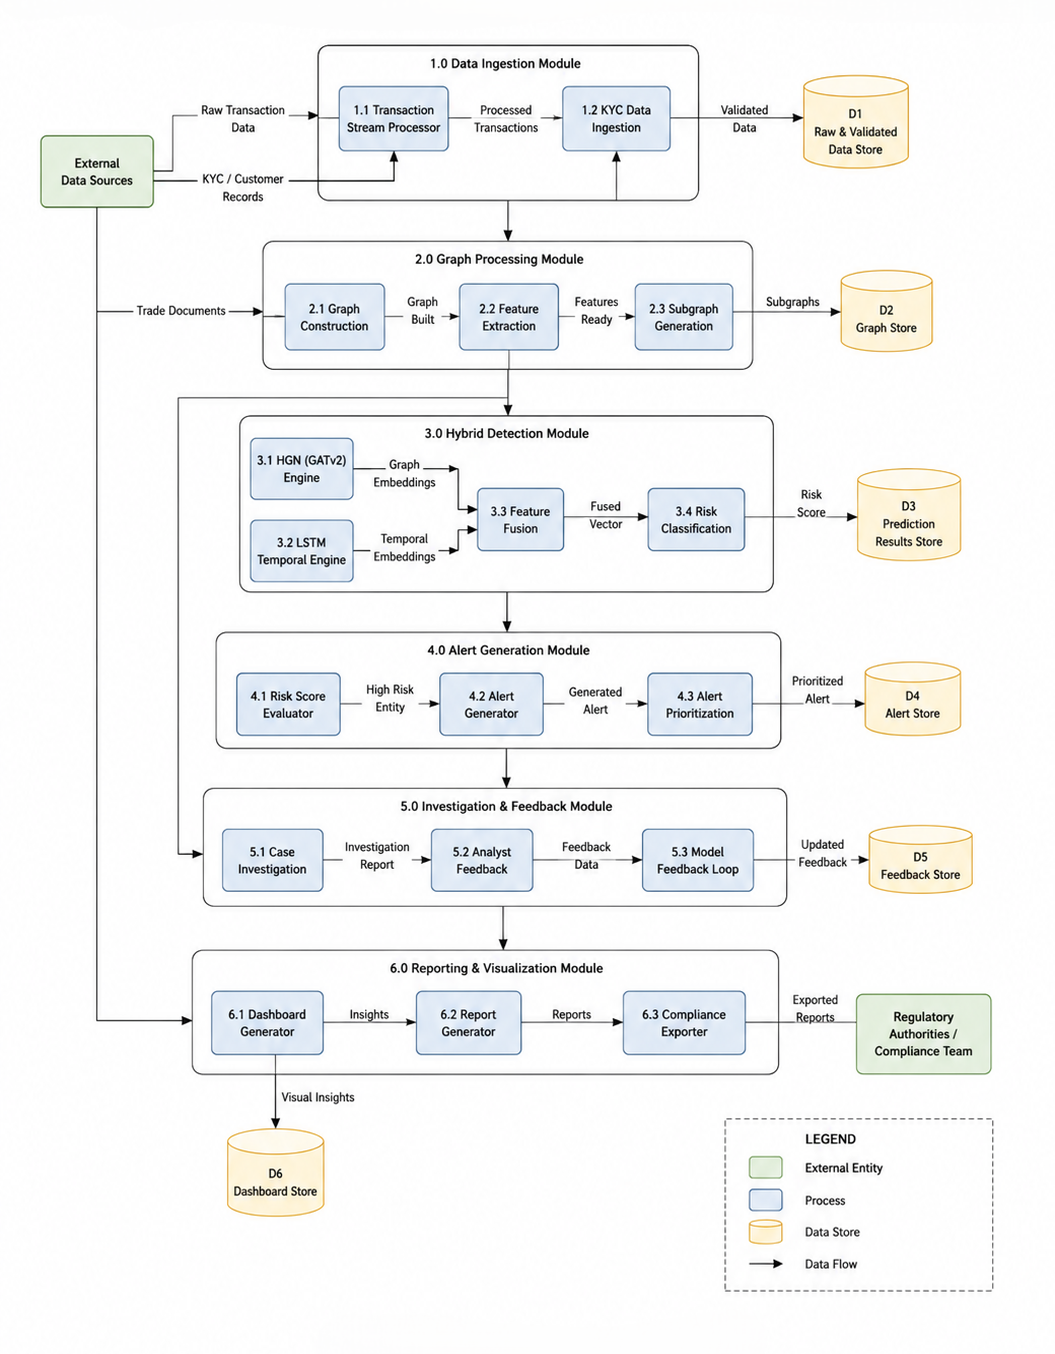
\includegraphics[
        width=\textwidth,
        height=0.9\textheight,
        keepaspectratio
    ]{Figures/DFD_Level_2.png}
    \caption{Level 2 Data Flow Diagram}
    \label{fig:dfd_level2}
\end{figure}

Figure \ref{fig:dfd_level2}
depicts the Level 2 Data Flow Diagram showing the internal decomposition of the HGNN Fraud Detection module in the proposed framework.
The
initial stage of the process involves Data Integration and Validation, during which data from various sources related to trade invoices, shipments, and transaction
metadata is integrated and validated for discrepancies. The
valid data is fed into the Entity Resolution and Feature Extraction stage, where relational attributes are identified, and financial contextual features are extracted
for the purposes of graph-based learning. The next process stage involves Heterogeneous Graph Generation, where interconnected financial transaction graphs
are created, containing the relevant information about entities, accounts, invoices, and trade relations. The HGNN Inference and Risk Scoring module utilizes
graph-based neural network learning to determine anomaly scores and detect any suspicious transaction patterns. The results of this analysis are processed
by the Anomaly Detection and Classification module, followed by the Alert Generation and Prioritization module, where suspicious activities are prioritized based on
risk levels. Finally, the Result Aggregation and Reporting module prepares a report of the detected fraudulent activities, suspicious transaction patterns, and
analytical results and forwards it to the Alert and Monitoring Dashboard module.


%========================================================
\section{Summary}
%========================================================
In this chapter, the high-level architecture of the proposed Federated Heterogeneous Graph Neural Network (HGNN)-Based TBML Detection Framework is described. Design issues involved scaling, privacy preservation, modularity, transaction monitoring, and secure collaboration among institutions in a distributed environment. Besides the discussion of design issues, the chapter explained how the design methodologies, architectural approaches, programming tools, and integration techniques used for the implementation of graph-based fraud detection, federated learning, and compliance monitoring were developed.
System Architecture
The complete system architecture revealed the integration of the processing of transactions, heterogeneity graph generation, hybrid graph neural networks, federated learning approach, and compliance environment for effective TBML detection. In addition, the level 0, level 1, and level 2 Data Flow Diagrams depicting the flow of financial transactions, internal processing, fraud detection, and alerts are provided in the chapter. All the architectural components combine together to provide a scalable and privacy-preserving monitoring system for anti-money laundering.

		
		%Chapter 5
		%========================================================
\chapter{Detailed Design of the Proposed TBML Framework}
%========================================================

The detailed design of the proposed TBML detection framework focuses on the internal organization, analytical workflow, and module-level interaction associated with graph-based fraud detection and real-time financial monitoring. The framework integrates transaction processing services, heterogeneous graph construction, hybrid HGNN--LSTM analytical models, federated learning mechanisms, and compliance reporting modules within a unified monitoring environment. This chapter presents the structure chart, detailed module design, database schema organization, and monitoring workflow associated with the proposed TBML detection framework.

%========================================================
\section[Structure Chart]{\textbf{Structure Chart}}
%========================================================
The structure chart of the proposed TBML detection framework illustrates the hierarchical organization of the major functional modules operating within the system. The framework is divided into frontend, backend, fraud detection, federated learning, database, and compliance layers to support scalable financial monitoring and intelligent fraud analysis within distributed Anti-Money Laundering environments.

The frontend layer provides dashboard interfaces, transaction monitoring services, risk visualization, and STR management functionalities for institutional users. Backend services coordinate API communication, transaction processing, authentication workflows, and access control operations between frontend interfaces and analytical modules. The fraud detection layer incorporates Hybrid HGNN--LSTM components responsible for graph-based analysis, temporal transaction modeling, feature fusion, and risk classification.

The federated learning layer enables privacy-preserving collaborative model training and global model synchronization between participating institutions. Database services manage transactional storage, graph relationships, audit logs, and compliance-related records, while the compliance layer supports STR generation, regulatory reporting, email notifications, and monitoring operations. The overall structural organization of the proposed TBML detection framework is illustrated in Figure~\ref{fig:structure_chart}.
\begin{figure}[H]
    \centering
    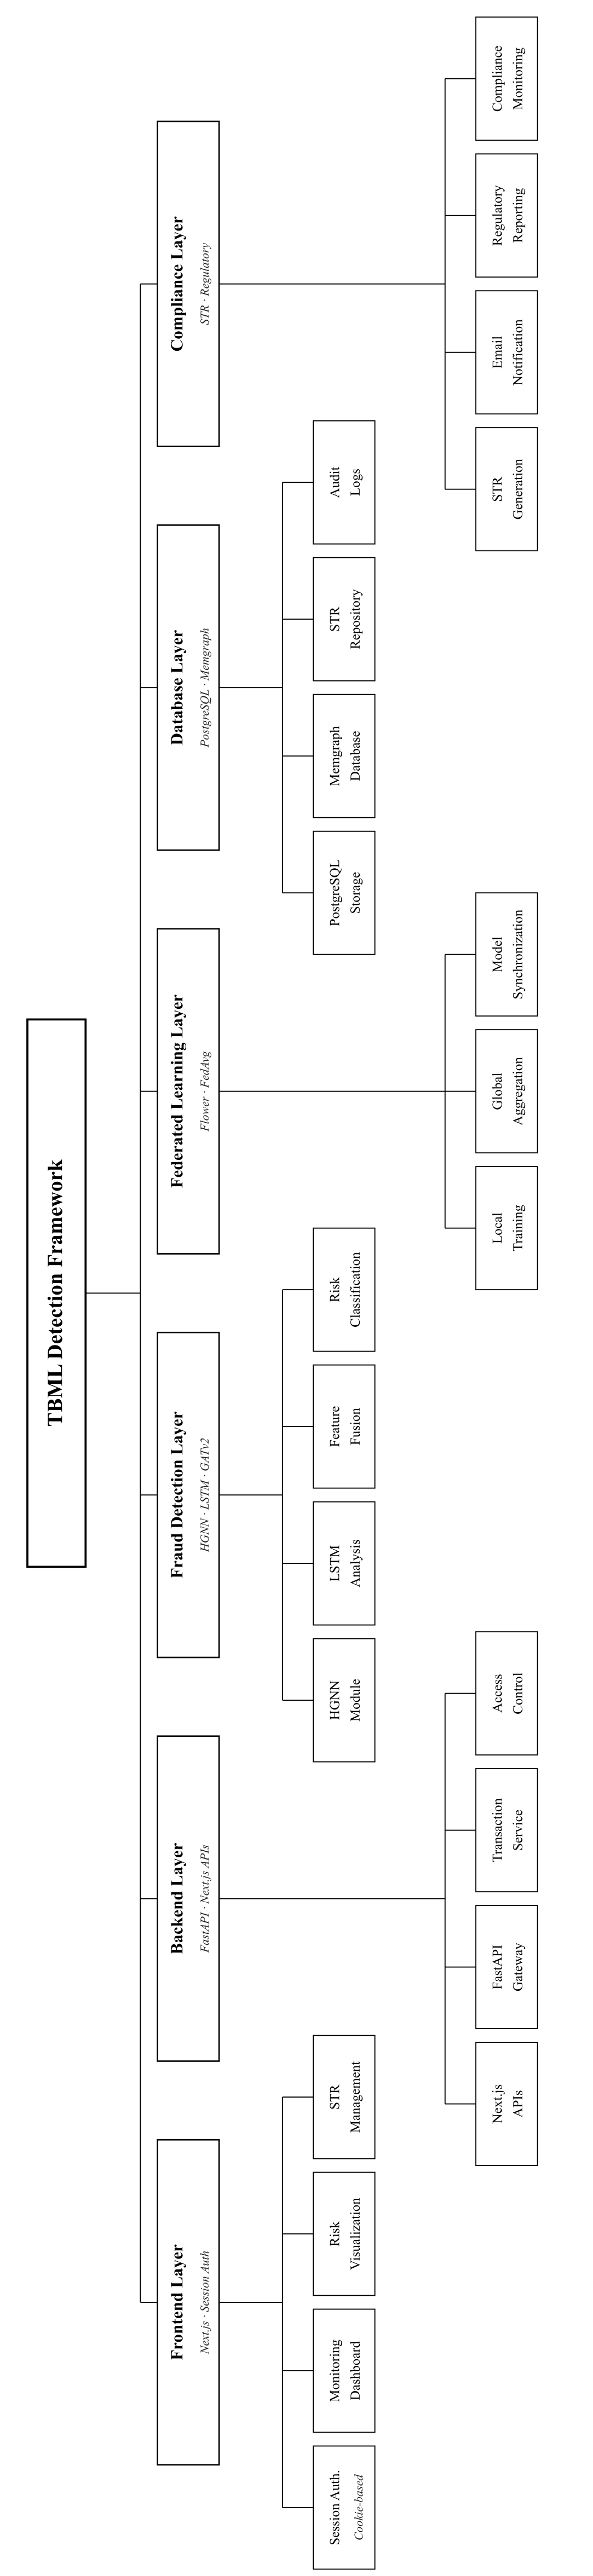
\includegraphics[height=0.95\textheight]{Figures/tbml_final_academic_structure_chart.png}
    \caption{Structure Chart of the Proposed TBML Detection Framework}
    \label{fig:structure_chart}
\end{figure}

The structure chart illustrates the modular organization and interaction between analytical, monitoring, storage, and compliance-oriented services within the proposed framework. This modular design approach improves scalability, maintainability, service integration, and efficient coordination between frontend interfaces, backend analytical services, and distributed fraud detection environments.

%========================================================
\section[Functional Description of the Modules]{\textbf{Functional Description of the Modules}}
%========================================================

The functional description of the modules explains the internal processing workflow and interaction between the major analytical, monitoring, and compliance-oriented components operating within the proposed TBML detection framework. The framework integrates transaction streaming services, graph construction mechanisms, hybrid HGNN--LSTM analytical models, institutional verification environments, and regulatory reporting systems to support intelligent Trade-Based Money Laundering detection and real-time compliance monitoring.

%========================================================
\subsection[Module Interaction Workflow]{\textbf{Module Interaction Workflow}}
%========================================================

The module interaction workflow illustrates the coordinated operational flow between transaction ingestion services, streaming environments, graph-based analytical modules, fraud classification mechanisms, institutional verification procedures, and regulatory monitoring systems functioning within the proposed framework. Financial transactions, KYC records, and trade documents are initially processed within the transaction processing layer and published into Kafka streaming topics for asynchronous event-driven communication between backend analytical services.

Kafka consumer services subsequently consume the transaction streams and forward the processed data to the graph construction and feature extraction module where heterogeneous financial transaction graphs are generated using accounts, transactions, trade entities, and document relationships stored within the Memgraph database. The extracted graph embeddings and relational features are processed by the Hybrid HGNN--LSTM fraud detection module to perform graph representation learning, temporal transaction analysis, and intelligent fraud prediction.

The generated fraud classifications and monitoring results are stored within the PostgreSQL database and visualized through the dashboard monitoring environment for institutional investigators and banking administrators. Suspicious transactions identified by the analytical system are reviewed by authorized bank administrators before being categorized as clean, suspicious, or confirmed fraudulent transactions.

Transactions verified as fraudulent are forwarded to the STR generation environment where Suspicious Transaction Reports are generated with analytical assistance from the Groq API service. Generated STR reports are subsequently reviewed by regulatory authorities responsible for investigation management, inquiry procedures, and enforcement operations. Notification management services coordinate fraud alerts and institutional communication processes, while the Resend email service delivers notification emails and regulatory enforcement messages to the corresponding institutional authorities. The overall module interaction workflow of the proposed TBML detection framework is illustrated in Figure~\ref{fig:workflow_interaction}.

\begin{figure}[H]
    \centering
    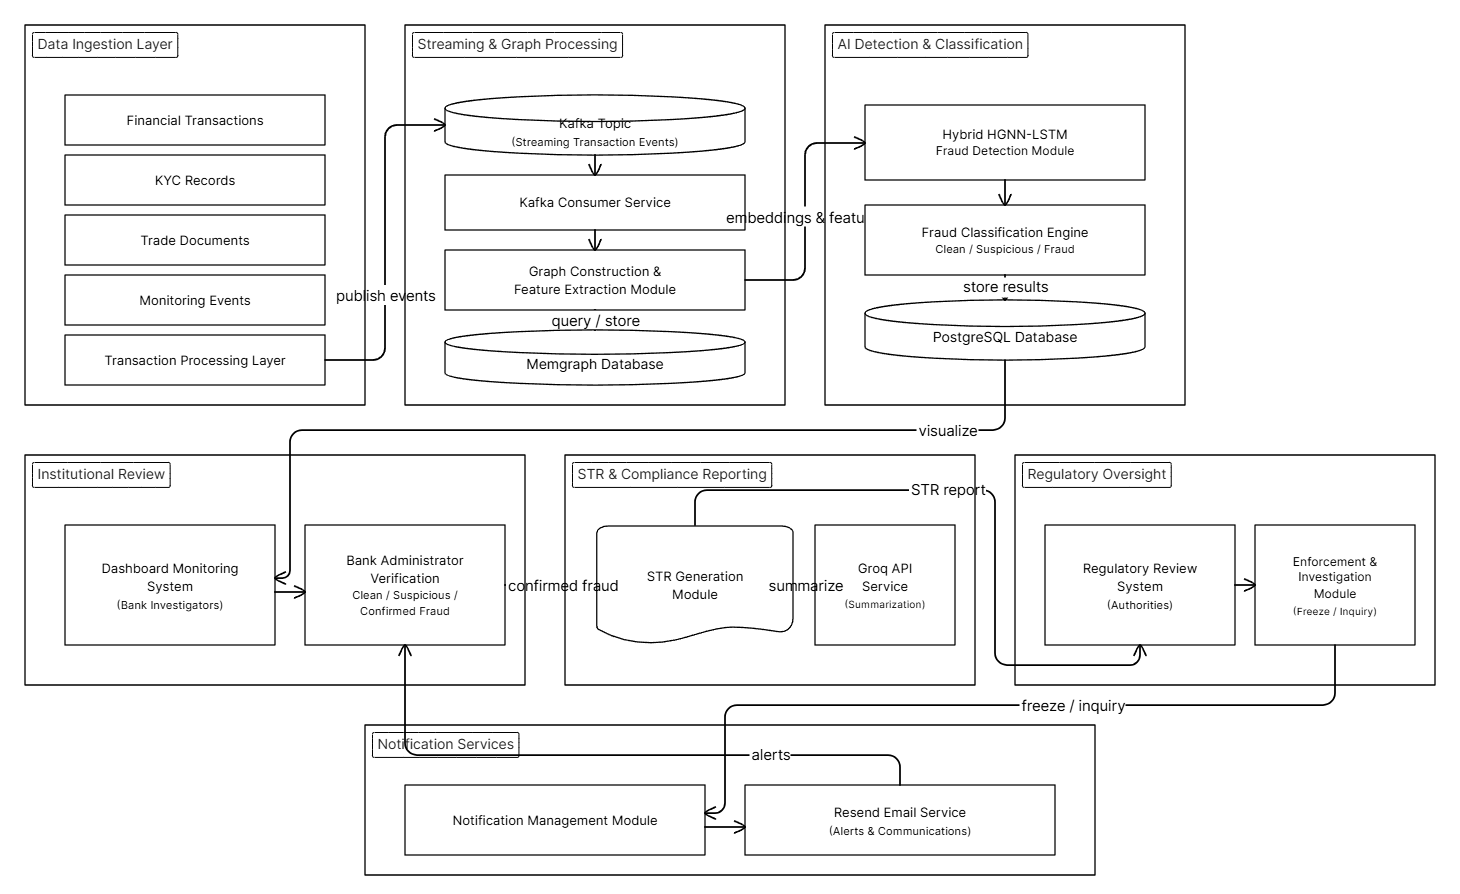
\includegraphics[width=\textwidth]{Figures/module-interaction2.png}
    \caption{Workflow Interaction Diagram for the Proposed TBML Detection Framework}
    \label{fig:workflow_interaction}
\end{figure}

The workflow interaction diagram illustrates the coordinated interaction between streaming services, graph-based analytical modules, monitoring environments, institutional verification systems, and regulatory compliance services operating within the proposed framework. Such modular workflow integration supports scalable transaction processing, intelligent fraud analysis, compliance management, and real-time Anti-Money Laundering monitoring within distributed financial environments.

%========================================================
\subsection[Transaction Processing Module]{\textbf{Transaction Processing Module}}
%========================================================

The transaction processing Module acts as the initial ingestion environment within the proposed TBML detection framework. This Module collects financial transactions, KYC records, trade documents, and institutional monitoring events originating from banking systems and external financial environments.

The input data processed within this Module includes sender and receiver account identifiers, transaction amounts, commodity types, trade quantities, trade values, invoice details, transaction timestamps, and institutional monitoring attributes associated with financial activities. The collected transactional data is validated, normalized, and converted into structured transaction records to support reliable downstream analytical processing.

The processed transaction events are published into Kafka streaming topics to enable asynchronous communication between backend services and analytical modules. The generated transaction streams serve as the primary input for graph construction, feature extraction, and graph-based fraud detection operations within the proposed framework.


%========================================================
\subsection[Graph Construction Module]{\textbf{Graph Construction Module}}
%========================================================

The graph construction module is responsible for transforming processed transaction streams into heterogeneous financial transaction graphs for graph-based analytical processing. This module receives validated transaction events from Kafka consumer services and models financial interactions between accounts, transactions, trade documents, and institutional entities within a connected graph environment.

The generated graph schema consists of interconnected node entities including \texttt{(:Account)}, \texttt{(:Transaction)}, and \texttt{(:Document)} connected through graph relationships such as \texttt{[:SENDS]}, \texttt{[:TO]}, and \texttt{[:HAS\_DOC]}. These relationships represent sender-receiver interactions, transaction ownership, trade associations, and document linkages required for identifying hidden transactional dependencies associated with Trade-Based Money Laundering activities.

The module interacts with the Memgraph database to store graph structures, entity relationships, and transactional connectivity information required for downstream analytical learning. The generated graph features and relational representations are subsequently forwarded to the Hybrid HGNN--LSTM fraud detection module for graph-based fraud analysis and intelligent transaction classification.

%========================================================
\subsection[Hybrid HGNN--LSTM Fraud Detection Module]{\textbf{Hybrid HGNN--LSTM Fraud Detection Module}}
%========================================================

The Hybrid HGNN--LSTM fraud detection module performs graph-based fraud analysis and temporal transaction modeling within the proposed TBML detection framework. The module receives KYC node features, transaction sequences, SWIFT edge attributes, and trade metadata generated from the graph construction environment for downstream analytical processing.

The graph branch utilizes multi-layer GATv2 operations to perform neighborhood aggregation and graph attention learning across interconnected financial entities. In parallel, the temporal branch utilizes LSTM-based sequential modeling to analyze transaction sequences and identify abnormal temporal transaction behavior associated with suspicious financial activities. The trade branch processes trade metadata and institutional transaction attributes using multilayer perceptron operations and feature normalization mechanisms.

The generated graph embeddings, temporal representations, and trade feature vectors are combined within the feature fusion layer for downstream fraud prediction and transaction risk analysis. The dense classification layer categorizes transactions into predefined classes including \texttt{CLEAN}, \texttt{WATCHLIST}, and \texttt{FRAUD}. The overall architecture of the proposed Hybrid HGNN--LSTM fraud detection module is illustrated in Figure~\ref{fig:hgnn_architecture}.

\begin{figure}[H]
    \centering
    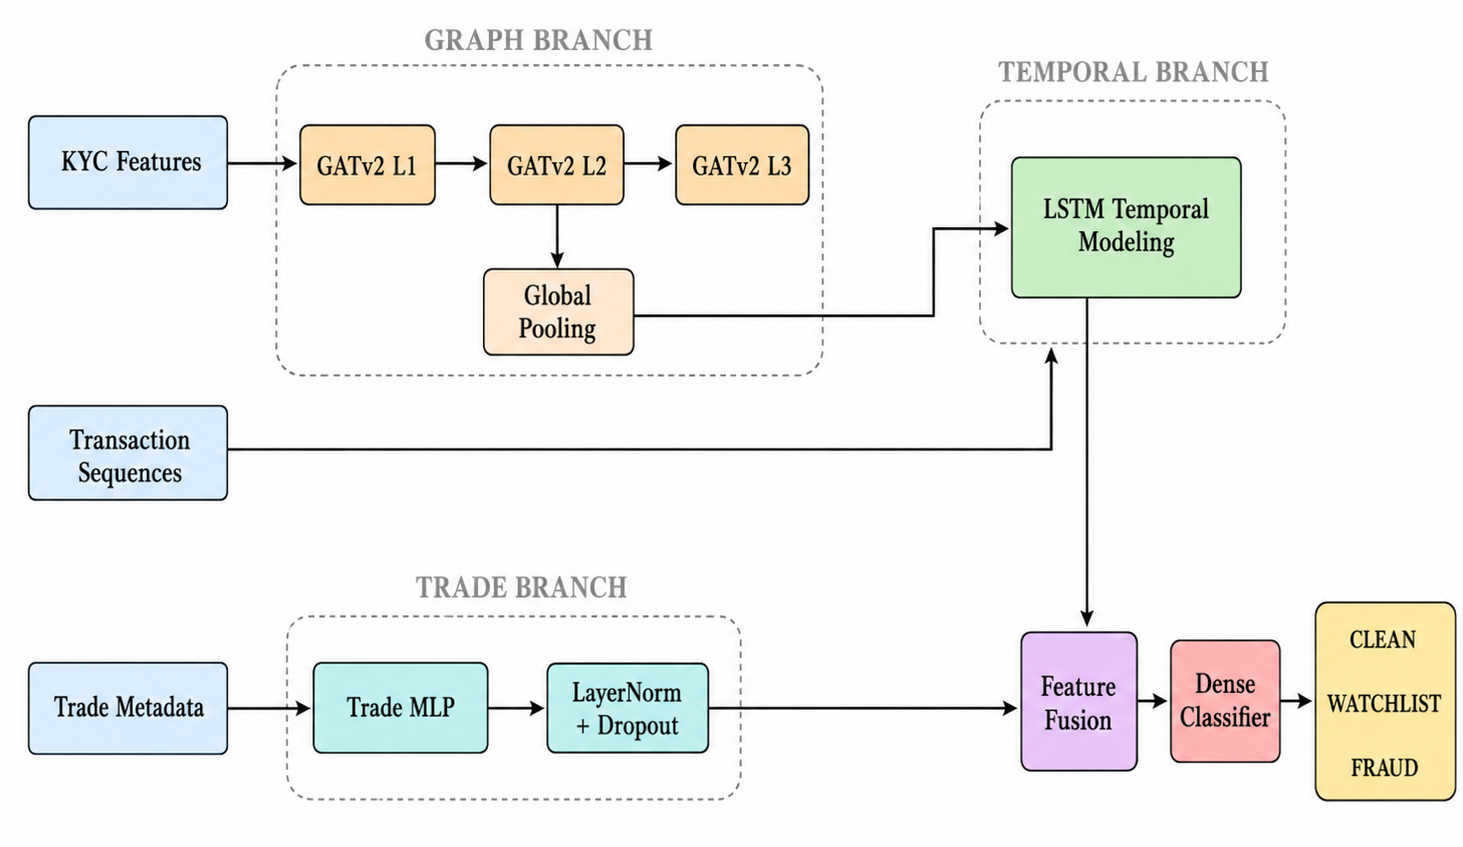
\includegraphics[width=\textwidth]{Figures/aimodel.png}
    \caption{Architecture of the Proposed Hybrid HGNN--LSTM Fraud Detection Module}
    \label{fig:hgnn_architecture}
\end{figure}



%========================================================
\subsection[Federated Learning Module]{\textbf{Federated Learning Module}}
%========================================================

The federated learning module enables privacy-preserving collaborative fraud detection across distributed financial institutions without directly sharing sensitive transactional data. Each participating institution performs local model training using institutional transaction graphs, transaction sequences, and fraud classification labels generated within the analytical environment.

The locally trained model parameters are periodically transmitted to the central aggregation server where the Federated Averaging (\texttt{FedAvg}) strategy combines local model updates to generate an optimized global fraud detection model. The aggregated global model is subsequently redistributed to participating institutions for continuous fraud detection and real-time analytical inference. The overall federated learning architecture of the proposed framework is illustrated in Figure~\ref{fig:federated_architecture}.

\begin{figure}[H]
    \centering
    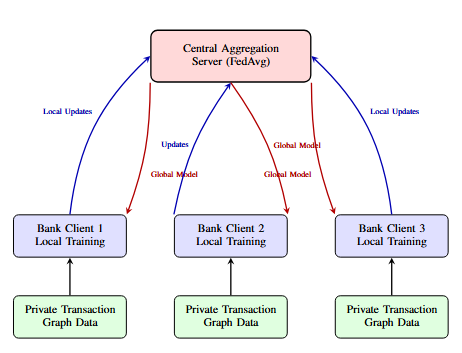
\includegraphics[width=0.82\textwidth]{Figures/federated_architecture.png}
    \caption{Federated learning architecture for privacy-preserving collaborative TBML detection across distributed institutions}
    \label{fig:federated_architecture}
\end{figure}



%========================================================
\subsubsection[STR Generation and Notification Module]{\textbf{STR Generation and Notification Module}}
%========================================================

The STR generation and notification module is responsible for compliance reporting and fraud alert management within the proposed TBML detection framework. Transactions verified as fraudulent by authorized banking administrators are forwarded to this module for Suspicious Transaction Report (STR) generation and regulatory processing. The module generates STR reports containing transaction details, fraud classifications, trade metadata, institutional information, and investigation summaries associated with suspicious financial activities.

The Groq API service is utilized for analytical summarization and automated assistance during compliance documentation generation. Generated STR reports are subsequently forwarded to regulatory monitoring authorities for investigation and enforcement procedures. The notification management environment coordinates fraud alerts and institutional communication workflows, while the Resend email service delivers notification emails, investigation alerts, and regulatory enforcement messages to banking institutions and regulatory authorities.
%========================================================
\subsubsection[Dashboard and Regulatory Monitoring Module]{\textbf{Dashboard and Regulatory Monitoring Module}}
%========================================================

The dashboard and regulatory monitoring module provides real-time transaction visualization, fraud monitoring, and institutional investigation functionalities within the proposed TBML detection framework. The monitoring dashboard displays transaction classifications, fraud alerts, risk scores, STR records, and analytical monitoring information generated by the fraud detection environment. Separate dashboard environments are maintained for banking administrators and regulatory authorities to support institution-level monitoring and centralized compliance management operations.

Authorized banking administrators can view suspicious and fraudulent transactions identified by the analytical model and perform institutional verification procedures before categorizing transactions as \texttt{CLEAN}, \texttt{WATCHLIST}, or \texttt{FRAUD}. Suspicious transactions can either be escalated as fraudulent transactions or marked as clean after institutional verification procedures, thereby reducing false positive classifications within the monitoring environment. Transactions verified as fraudulent are subsequently forwarded for Suspicious Transaction Report (STR) generation and regulatory reporting.

Regulatory authorities monitor generated STR reports and institution-level fraud cases through centralized monitoring dashboards. The regulatory environment supports compliance monitoring, document verification requests, inquiry procedures, and account freeze operations associated with suspicious financial activities.




% %========================================================
% \section[Sequence Diagram for TBML Detection Workflow]{\textbf{Sequence Diagram for TBML Detection Workflow}}
% %========================================================

% The sequence diagram illustrates the dynamic interaction between the major system components involved in transaction monitoring, graph-based fraud analysis, federated learning, and compliance alert generation within the proposed TBML detection framework. The workflow begins when the monitoring dashboard initiates a transaction monitoring request through the banking environment. Transaction events are streamed and forwarded to the graph construction module where heterogeneous graph structures and analytical features are generated for fraud analysis.

% The generated graph data is processed by the Hybrid HGNN--LSTM analytical model to perform graph representation learning and temporal transaction analysis. Local model updates generated during training are transmitted to the federated learning server where global aggregation and model synchronization are performed using federated averaging mechanisms. The updated global model is subsequently utilized by the detection engine to perform fraud inference, generate risk classifications, and identify suspicious transactional behavior.

% Once suspicious activity is detected, the STR and notification service generates compliance reports and triggers alert notifications for institutional monitoring environments. The overall interaction flow between the major components of the proposed TBML detection framework is illustrated in Figure~\ref{fig:sequence_diagram}.

% \begin{figure}[H]
%     \centering
%     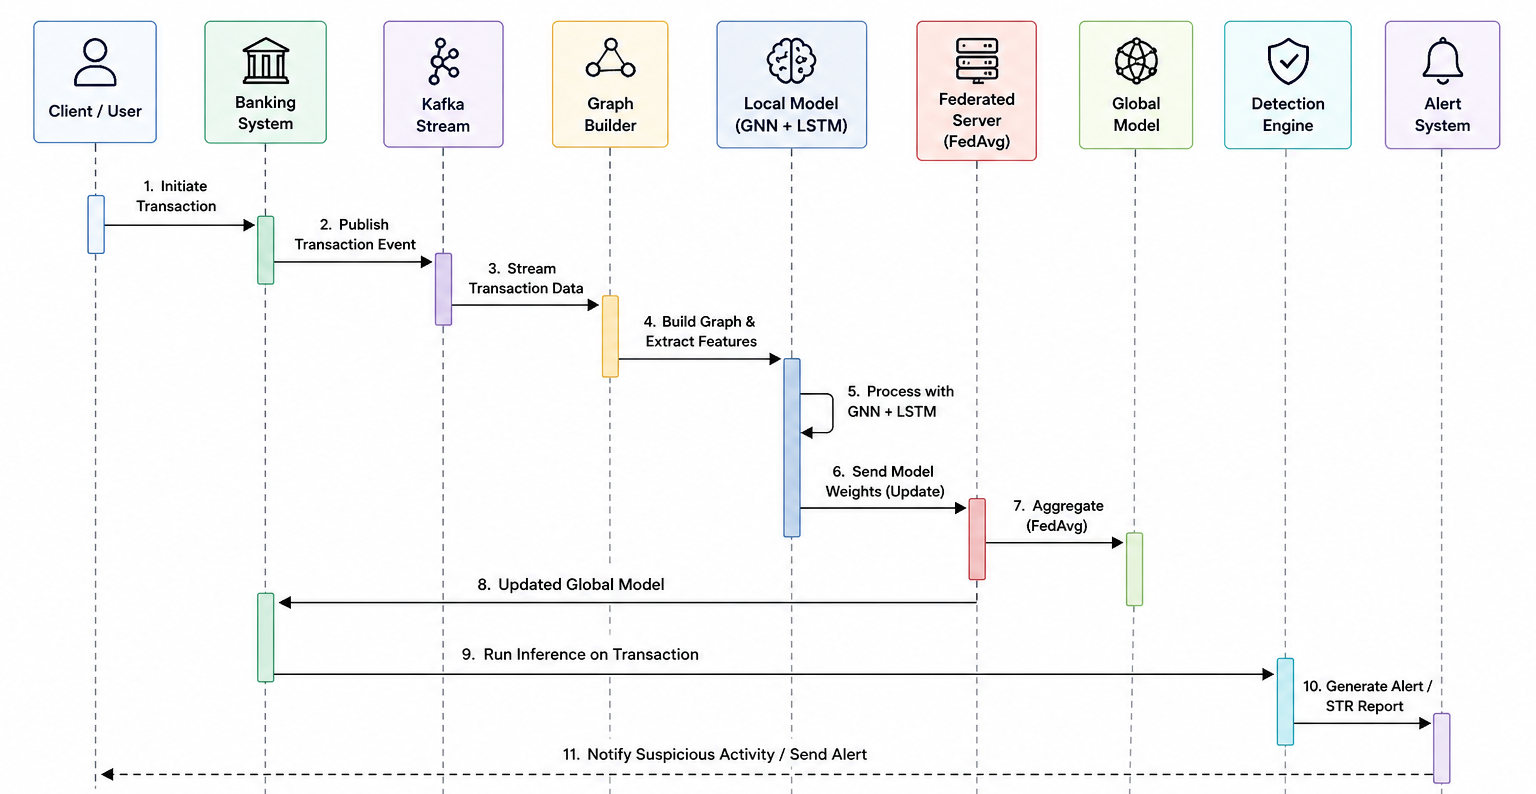
\includegraphics[width=\textwidth]{Figures/sequencediagramfinal.png}
%     \caption{Sequence Diagram for TBML Detection Workflow}
%     \label{fig:sequence_diagram}
% \end{figure}

% The sequence diagram demonstrates the coordinated interaction between frontend interfaces, transaction streaming services, analytical modules, federated learning environments, and compliance reporting systems operating within the proposed framework. Such coordinated workflows enable scalable real-time fraud detection, privacy-preserving collaborative learning, and efficient Anti-Money Laundering monitoring operations.
% %========================================================
% \section[Database Schema Design]{\textbf{Database Schema Design}}
% %========================================================



%========================================================
\section[Summary]{\textbf{Summary}}
%========================================================

This chapter presented the detailed design of the proposed TBML detection framework including the structural organization, module interaction workflow, functional description of analytical modules, federated learning architecture, and database management environment associated with the system. The chapter discussed the interaction between transaction processing services, graph construction mechanisms, hybrid HGNN--LSTM analytical modules, dashboard monitoring environments, and compliance reporting systems operating within the proposed framework.

The detailed design further illustrated how streaming-based transaction processing, graph-based fraud analysis, federated collaborative learning, institutional verification, STR generation, and regulatory monitoring are integrated within a unified Anti-Money Laundering environment. The subsequent chapter discusses the implementation details, backend integration and dashboard development associated with the proposed TBML detection framework.
		
		 % %Chapter 6
		%========================================================
\chapter{Implementation and Testing of the Proposed TBML Detection Framework}
%========================================================

This chapter details the implementation of the FedGAT-TBML framework. It covers real-time transaction ingestion and streaming, construction and storage of heterogeneous transaction graphs, a hybrid HGNN--LSTM detector for sequence-aware graph inference, federated learning orchestration for privacy-preserving model updates, and a web dashboard for compliance monitoring and STR generation. The implementation leverages Apache Kafka for durable streaming, Memgraph for graph storage and queries, PostgreSQL for audit and STR records, PyTorch Geometric for graph neural network components (e.g., GATv2Conv), Flower for federated orchestration, FastAPI for backend services, and Next.js/TypeScript for the frontend.

%========================================================
\section{Implementation }
%========================================================
This section provides a comprehensive overview of the implementation of the proposed TBML detection framework, detailing the programming languages, frameworks, platforms, code conventions, system architecture, and the strategies employed to address implementation challenges. The implementation integrates real-time transaction streaming, heterogeneous graph construction, hybrid analytical modeling, federated learning coordination, and compliance monitoring within a unified platform for effective Trade-Based Money Laundering detection and institutional oversight.

%========================================================
\subsection[Programming Language and Framework Selection]{\textbf{Programming Language and Framework Selection}}
%========================================================

The implementation primarily uses Python for backend services and model training (PyTorch + PyTorch Geometric — e.g., \texttt{GATv2Conv} for graph attention), Flower for federated orchestration (custom \texttt{FedAvg} strategy), and Apache Kafka for durable streaming. Frontend and UI services use Next.js, TypeScript and Tailwind; FastAPI provides REST endpoints. Memgraph stores heterogeneous transaction graphs and PostgreSQL holds audit logs and STR records. Services are containerized with Docker for reproducible deployment.

%========================================================
\subsection[Platform Selection]{\textbf{Platform Selection}}
%========================================================

The proposed TBML detection framework is developed within a Windows-based  environment consisting of interconnected frontend monitoring services and backend analytical infrastructures. The frontend platform manages authentication workflows, dashboard visualization, STR generation, regulatory monitoring, and institutional transaction management, while the backend analytical environment performs transaction streaming, graph generation, fraud inference, and federated model synchronization operations.

The implementation utilizes Docker-based isolated runtime environments for Kafka services, graph databases, backend APIs, and federated learning modules to improve deployment consistency and distributed service orchestration. Memgraph is utilized for graph relationship management and transactional connectivity analysis, whereas PostgreSQL functions as the centralized synchronization database between analytical services and dashboard environments. Visual Studio Code and GitHub are utilized for collaborative development, source-code management, debugging, and version control operations throughout the implementation lifecycle.

%========================================================
\subsection[Code Conventions]{\textbf{Code Conventions}}
%========================================================

The codebase follows concise, practical conventions to improve readability and maintenance. Python modules and functions use \texttt{snake\_case}; classes and UI components use \texttt{PascalCase}. Examples of graph entities and relationships include \texttt{(:Account)}, \texttt{(:Transaction)}, \texttt{(:Document)} and \texttt{[:SENDS]}, \texttt{[:TO]}, \texttt{[:HAS\_DOC]}. REST endpoints follow clear, resource-oriented naming (e.g., \texttt{/api/transactions/\{id\}/score}). Configuration is managed via \texttt{.env} files, logging uses structured JSON logs, and type hints plus docstrings are used where helpful.

%========================================================
\subsubsection[Naming Conventions]{\textbf{Naming Conventions}}
%========================================================

Naming conventions within the proposed framework are designed to remain semantically meaningful and aligned with domain-specific financial monitoring operations. Python variables, backend utility functions, Kafka services, and transaction-processing modules follow \texttt{snake\_case} conventions, whereas analytical classes, federated learning modules, and frontend components utilize \texttt{PascalCase} notation. REST API endpoints, transaction services, and graph-processing utilities are named according to their operational functionality to improve implementation readability and maintainability.

Graph entities, transactional relationships, and database schemas additionally follow consistent naming conventions across graph and relational database environments. Examples include graph entities such as \texttt{(:Account)}, \texttt{(:Transaction)}, and \texttt{(:Document)}, along with transactional relationships including \texttt{[:SENDS]}, \texttt{[:TO]}, and \texttt{[:HAS\_DOC]} utilized throughout graph construction and fraud analysis operations.

% %========================================================
% \subsubsection[File Organization]{\textbf{File Organization}}
% %========================================================

% The proposed TBML detection framework follows a modular project structure where frontend monitoring services and backend analytical environments are maintained as interconnected distributed applications. The frontend environment contains dashboard interfaces, authentication services, STR management workflows, API handlers, reusable UI components, and regulatory monitoring modules implemented using the Next.js App Router architecture and TypeScript-based service organization.

% The backend analytical environment contains Kafka producers and consumers, graph construction services, Hybrid HGNN--LSTM model implementations, federated learning clients, inference pipelines, and database synchronization utilities responsible for real-time fraud analysis and transaction monitoring operations. Shared configuration files, utility services, logging environments, and centralized database connectors are additionally organized according to functional responsibilities to improve scalability, maintainability, and distributed service coordination across the proposed framework.

% %========================================================
% \subsubsection[Environment Configuration and Logging]{\textbf{Environment Configuration and Logging}}
% %========================================================

% Environment variables and runtime configurations are securely managed using centralized \texttt{.env} configuration files to prevent direct exposure of API credentials, Kafka broker addresses, database configurations, authentication tokens, and federated learning parameters within the codebase. Backend services including Kafka consumers, Memgraph connectors, PostgreSQL clients, and fraud inference pipelines are initialized during runtime to support centralized service configuration and distributed analytical synchronization.

% Logging mechanisms are integrated throughout transaction streaming services, graph-processing environments, federated learning modules, backend APIs, and fraud inference pipelines to support runtime monitoring, debugging, audit traceability, and compliance management operations. Fraud classifications, transaction verdicts, confidence scores, STR generation events, and institutional monitoring activities are additionally logged within PostgreSQL environments for dashboard synchronization and regulatory investigation workflows.

%========================================================
\subsection[Difficulties Encountered and Strategies Used]{\textbf{Difficulties Encountered and Strategies Used to Tackle}}
%========================================================
Implementation challenges included noisy and imbalanced labels, large graph sizes and memory constraints, streaming latency, and privacy-preserving coordination across institutional clients. Mitigations applied in the implementation include class rebalancing and targeted data augmentation for scarce labels, subgraph sampling and mini-batching to control memory, Kafka buffering and asynchronous consumers to reduce end-to-end latency, and Flower with secure aggregation and containerized deployments (Docker) to isolate client environments while enabling federated training.


%========================================================
\subsection[System Implementation]{\textbf{System Implementation}}

%========================================================

The system implementation of the proposed TBML detection framework follows a distributed event-driven architecture integrating Kafka-based transaction streaming, heterogeneous graph generation, Hybrid HGNN--LSTM analytical processing, federated collaborative learning, real-time fraud inference, and dashboard-driven compliance monitoring. Backend analytical services, graph databases, inference pipelines, and frontend monitoring environments communicate through synchronized APIs, Kafka streams, and centralized PostgreSQL audit infrastructures to support scalable real-time Trade-Based Money Laundering detection and institutional monitoring operations.

\subsection[Synthetic Dataset Synthesis]{\textbf{Methodology of Synthetic Dataset Synthesis}}

The synthetic dataset was designed to mirror the complexity of real-world trade finance as closely as possible. It begins with a baseline network of financial entities, including Accounts, Documents, and Transactions, generated using power-law distributions so that the transaction volume looks more like an actual institutional environment. From there, the pipeline introduces temporal variation, commodity-specific price anomalies, and multi-currency layering patterns to create training data that is both structured and realistic.

The implementation follows a modular pipeline built with Pandas for data preparation and Memgraph for graph-based storage. Each transaction is linked to its corresponding trade document through a schema-consistent mapping so that the relationships needed for Graph Neural Network (GNN) feature extraction are preserved. With temporal constraints and controlled noise injection, the pipeline produces a broad range of behaviors, from ordinary legitimate trades to carefully concealed, high-velocity laundering patterns.

\subsubsection[Adversarial Refinement for Dataset Fidelity]{\textbf{Adversarial Refinement for Dataset Fidelity}}

To make the synthetic data behave more like real financial activity, the generation pipeline was refined with a set of adversarial and statistically grounded adjustments \cite{synthetic-tbml-framework}. The goal was to help the fraud-detection framework learn meaningful transactional and structural patterns instead of depending on easy shortcuts or deterministic signals.

\begin{enumerate}

    \item \textbf{Price Multiplier Dynamics:} Instead of using fixed pricing rules, the pipeline now uses Gaussian Mixture Models (GMMs) and stochastic blending so that some fraudulent trades look closer to genuine market behavior and are harder to catch with simple thresholds.

    \item \textbf{Elimination of Feature Bias:} The \textit{port\_log\_status} attribute was removed to prevent label leakage and push the Graph Neural Network to learn from relational and structural cues instead.

    \item \textbf{KYC/Dormancy Engineering:} Overlapping dormancy periods and controlled noise were added to produce customer activity patterns that feel more realistic than a simple dormant-versus-active split.

    \item \textbf{Universal Topology Injection:} Structures such as Cycles, Fan-In, and Gather-Scatter patterns were spread across all transaction classes so that no single graph shape automatically signals fraud.

    \item \textbf{Refined Pattern Classification:} Labels such as LEGIT and SUSPICIOUS were removed, and a neutral \textit{No\_Pattern} category was added so that structural topology stays separate from fraud labeling.

    \item \textbf{Temporal Realism:} The dataset was aligned to a realistic one-year operational timeline (Dec 2024--Dec 2025), with transaction durations modeled around practical financial activity windows.

    \item \textbf{Scale-Free Network Topology:} Pareto/Zipf-based node distributions were introduced to simulate high-volume institutional or ``Whale'' entities that can hide suspicious activity inside dense transaction networks.

    \item \textbf{Log-Normal Transaction Amounts:} Transaction values were generated with Log-Normal distributions so they better resemble real financial amounts instead of uniform synthetic values.

    \item \textbf{Multi-Hop Structural Integrity:} Rule-based constraints were applied across multi-hop paths to keep the graph consistent and preserve realistic relationship propagation.

    \item \textbf{FX Settlement/Currency-Jump Awareness:} Multi-currency flows and FX spread variations were added so the framework could learn cross-border layering and TBML settlement patterns.

    \item \textbf{Stochastic Trade Price Blending:} Illicit pricing distributions were blended with legitimate behavior to reduce obvious tabular shortcuts and encourage context-aware inference.

    \item \textbf{Data Leakage Mitigation:} Auxiliary indicators that could reveal fraud too directly were removed to improve generalization during training.

    \item \textbf{Endurance-Based Simulation:} Multi-hop cycles were modeled as sustained behaviors rather than isolated short-lived events to make the generated graph more realistic.

\end{enumerate}


%========================================================
\subsubsection[Kafka-Based Transaction Streaming]{\textbf{Kafka-Based Transaction Streaming}}
%========================================================

The proposed TBML detection framework utilizes Apache Kafka to support asynchronous transaction streaming and event-driven communication between distributed analytical services. A Kafka producer continuously generates synthetic SWIFT transaction payloads containing sender identifiers, receiver identifiers, transaction amounts, commodity information, trade quantities, price deviation scores, and weight-gap attributes before publishing them into the \texttt{incoming\_swift\_messages} topic for downstream analytical processing.

Kafka consumer services continuously subscribe to the transaction stream and process incoming financial events in real time for graph generation and fraud inference operations. The consumer pipeline validates transaction payloads, constructs heterogeneous graph relationships within Memgraph, extracts multi-hop transactional subgraphs, and forwards graph tensors to the Hybrid HGNN--LSTM inference engine for downstream fraud prediction and PostgreSQL audit logging. The streaming architecture enables decoupled communication between frontend services, graph-processing environments, and distributed analytical modules operating within the proposed framework.


%========================================================
\subsection[Graph Construction and Feature Extraction]{\textbf{Graph Construction and Feature Extraction}}
%========================================================

The graph construction pipeline transforms streamed financial transactions into heterogeneous graph representations for downstream graph-based analytical processing. Incoming transaction payloads consumed from the \texttt{incoming\_swift\_messages} Kafka topic are processed using Cypher-based graph ingestion operations within Memgraph, where transactional entities and financial relationships are dynamically mapped into interconnected graph structures as illustrated in Figure~\ref{fig:memgraph_graph}.

The generated graph schema consists of heterogeneous node entities including \texttt{(:Account)}, \texttt{(:Transaction)}, and \texttt{(:Document)} connected through relationships such as \texttt{[:SENDS]}, \texttt{[:TO]}, and \texttt{[:HAS\_DOC]}. The feature extraction pipeline subsequently performs constrained multi-hop subgraph traversal around the target transaction to generate node feature tensors, graph edge mappings, sequential transaction representations, and trade metadata tensors required for Hybrid HGNN--LSTM-based fraud inference operations.

\begin{figure}[H]
    \centering
    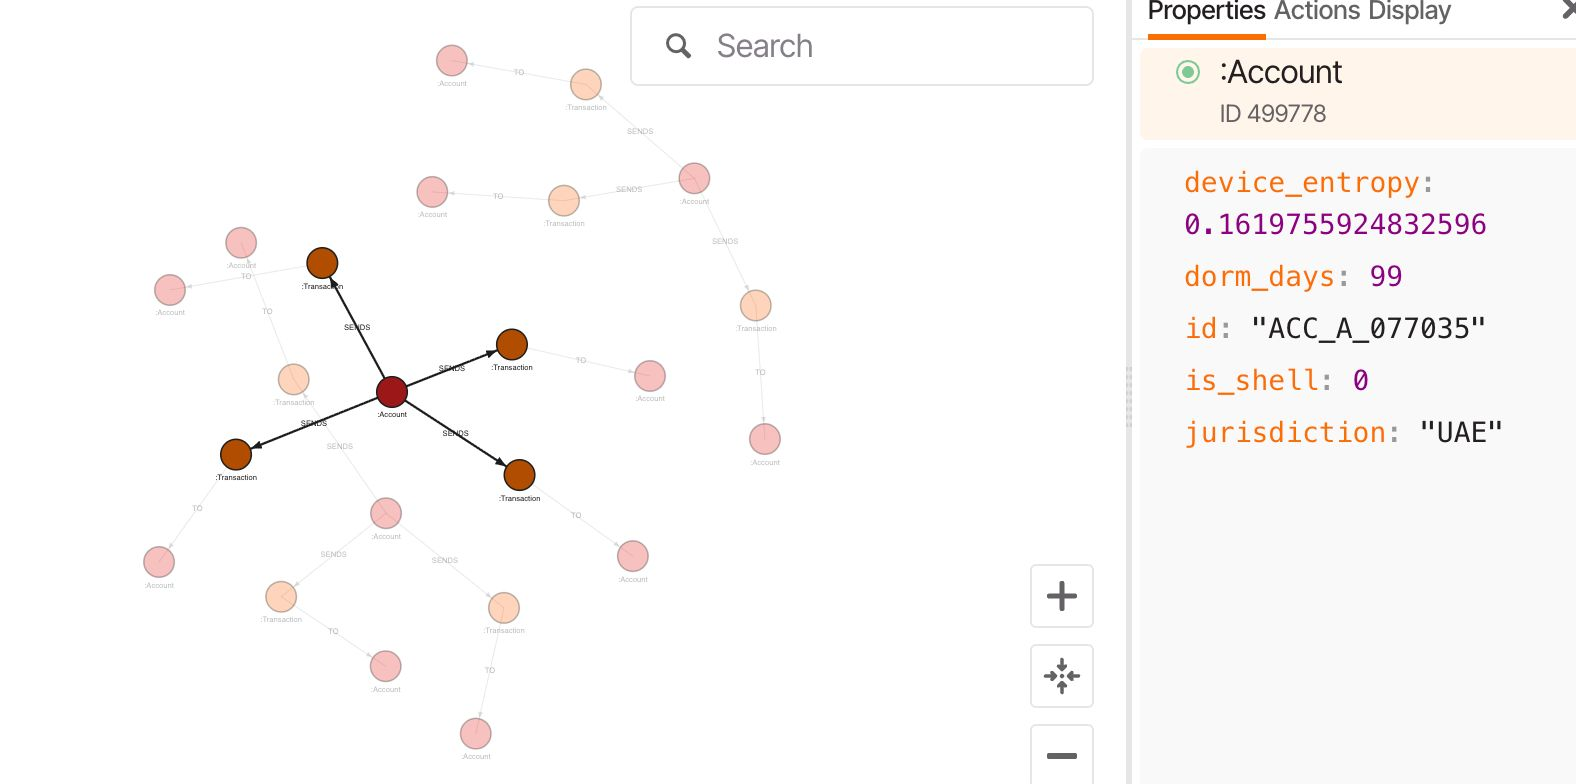
\includegraphics[width=0.95\textwidth]{Figures/memgraphlab.png}
    \caption{Heterogeneous financial transaction graph visualized within the Memgraph Lab environment.}
    \label{fig:memgraph_graph}
\end{figure}

%========================================================
\subsubsection[Hybrid HGNN--LSTM Analytical Implementation]{\textbf{Hybrid HGNN--LSTM Analytical Implementation}}
%========================================================

The proposed Hybrid HGNN--LSTM analytical module is implemented using PyTorch and PyTorch Geometric to perform graph-driven fraud analysis, temporal transaction modeling, and trade metadata learning for intelligent TBML detection. The implementation receives heterogeneous graph tensors generated from the Memgraph environment, including KYC node attributes, transactional edge relationships, sequential SWIFT transaction records, and trade-deviation features before forwarding them into the analytical inference pipeline. By combining graph attention learning with temporal sequence analysis and trade-feature fusion, the framework is capable of capturing both structural and behavioral fraud patterns across interconnected financial transaction networks.

The graph-learning branch utilizes a three-layer \texttt{GATv2Conv} architecture with multi-head attention mechanisms to perform neighborhood aggregation and graph message passing across interconnected financial entities \cite{brody2022gatv2}. The implemented graph layers process KYC-related node attributes such as shell-company indicators, jurisdiction metadata, and dormant-account characteristics to generate enriched graph embeddings capable of exposing hidden intermediary relationships and suspicious transaction-routing behavior. ReLU activation functions and dropout regularization are integrated after each graph convolution layer to improve representation stability during federated training operations. The generated graph embeddings are then aggregated using \texttt{global\_mean\_pool()} and fused with sequential SWIFT transaction features before being processed through the LSTM branch for temporal anomaly detection and sequential transaction behavior modeling. The temporal branch captures repeated payment structures, abnormal transaction timing behavior, and cyclic financial movement patterns that are difficult to identify using standalone graph-learning approaches.

Trade-specific metadata such as price-deviation attributes and cargo weight-gap indicators are independently processed using multilayer perceptron operations consisting of fully connected layers, Layer Normalization, ReLU activations, and dropout regularization mechanisms. The generated graph embeddings, temporal sequence representations, and trade-feature vectors are fused within the final analytical layer before being forwarded into the dense classification module for fraud prediction. The final classification layer categorizes transactions into predefined classes including \texttt{CLEAN}, \texttt{WATCHLIST}, and \texttt{FRAUD}. Experimental evaluation demonstrated stable federated convergence and strong fraud-class Precision--Recall performance across distributed institutional datasets. The overall implementation workflow of the proposed Hybrid HGNN--LSTM analytical module is illustrated in Figure~\ref{fig:hgnn_impl}.

\begin{figure}[H]
\centering

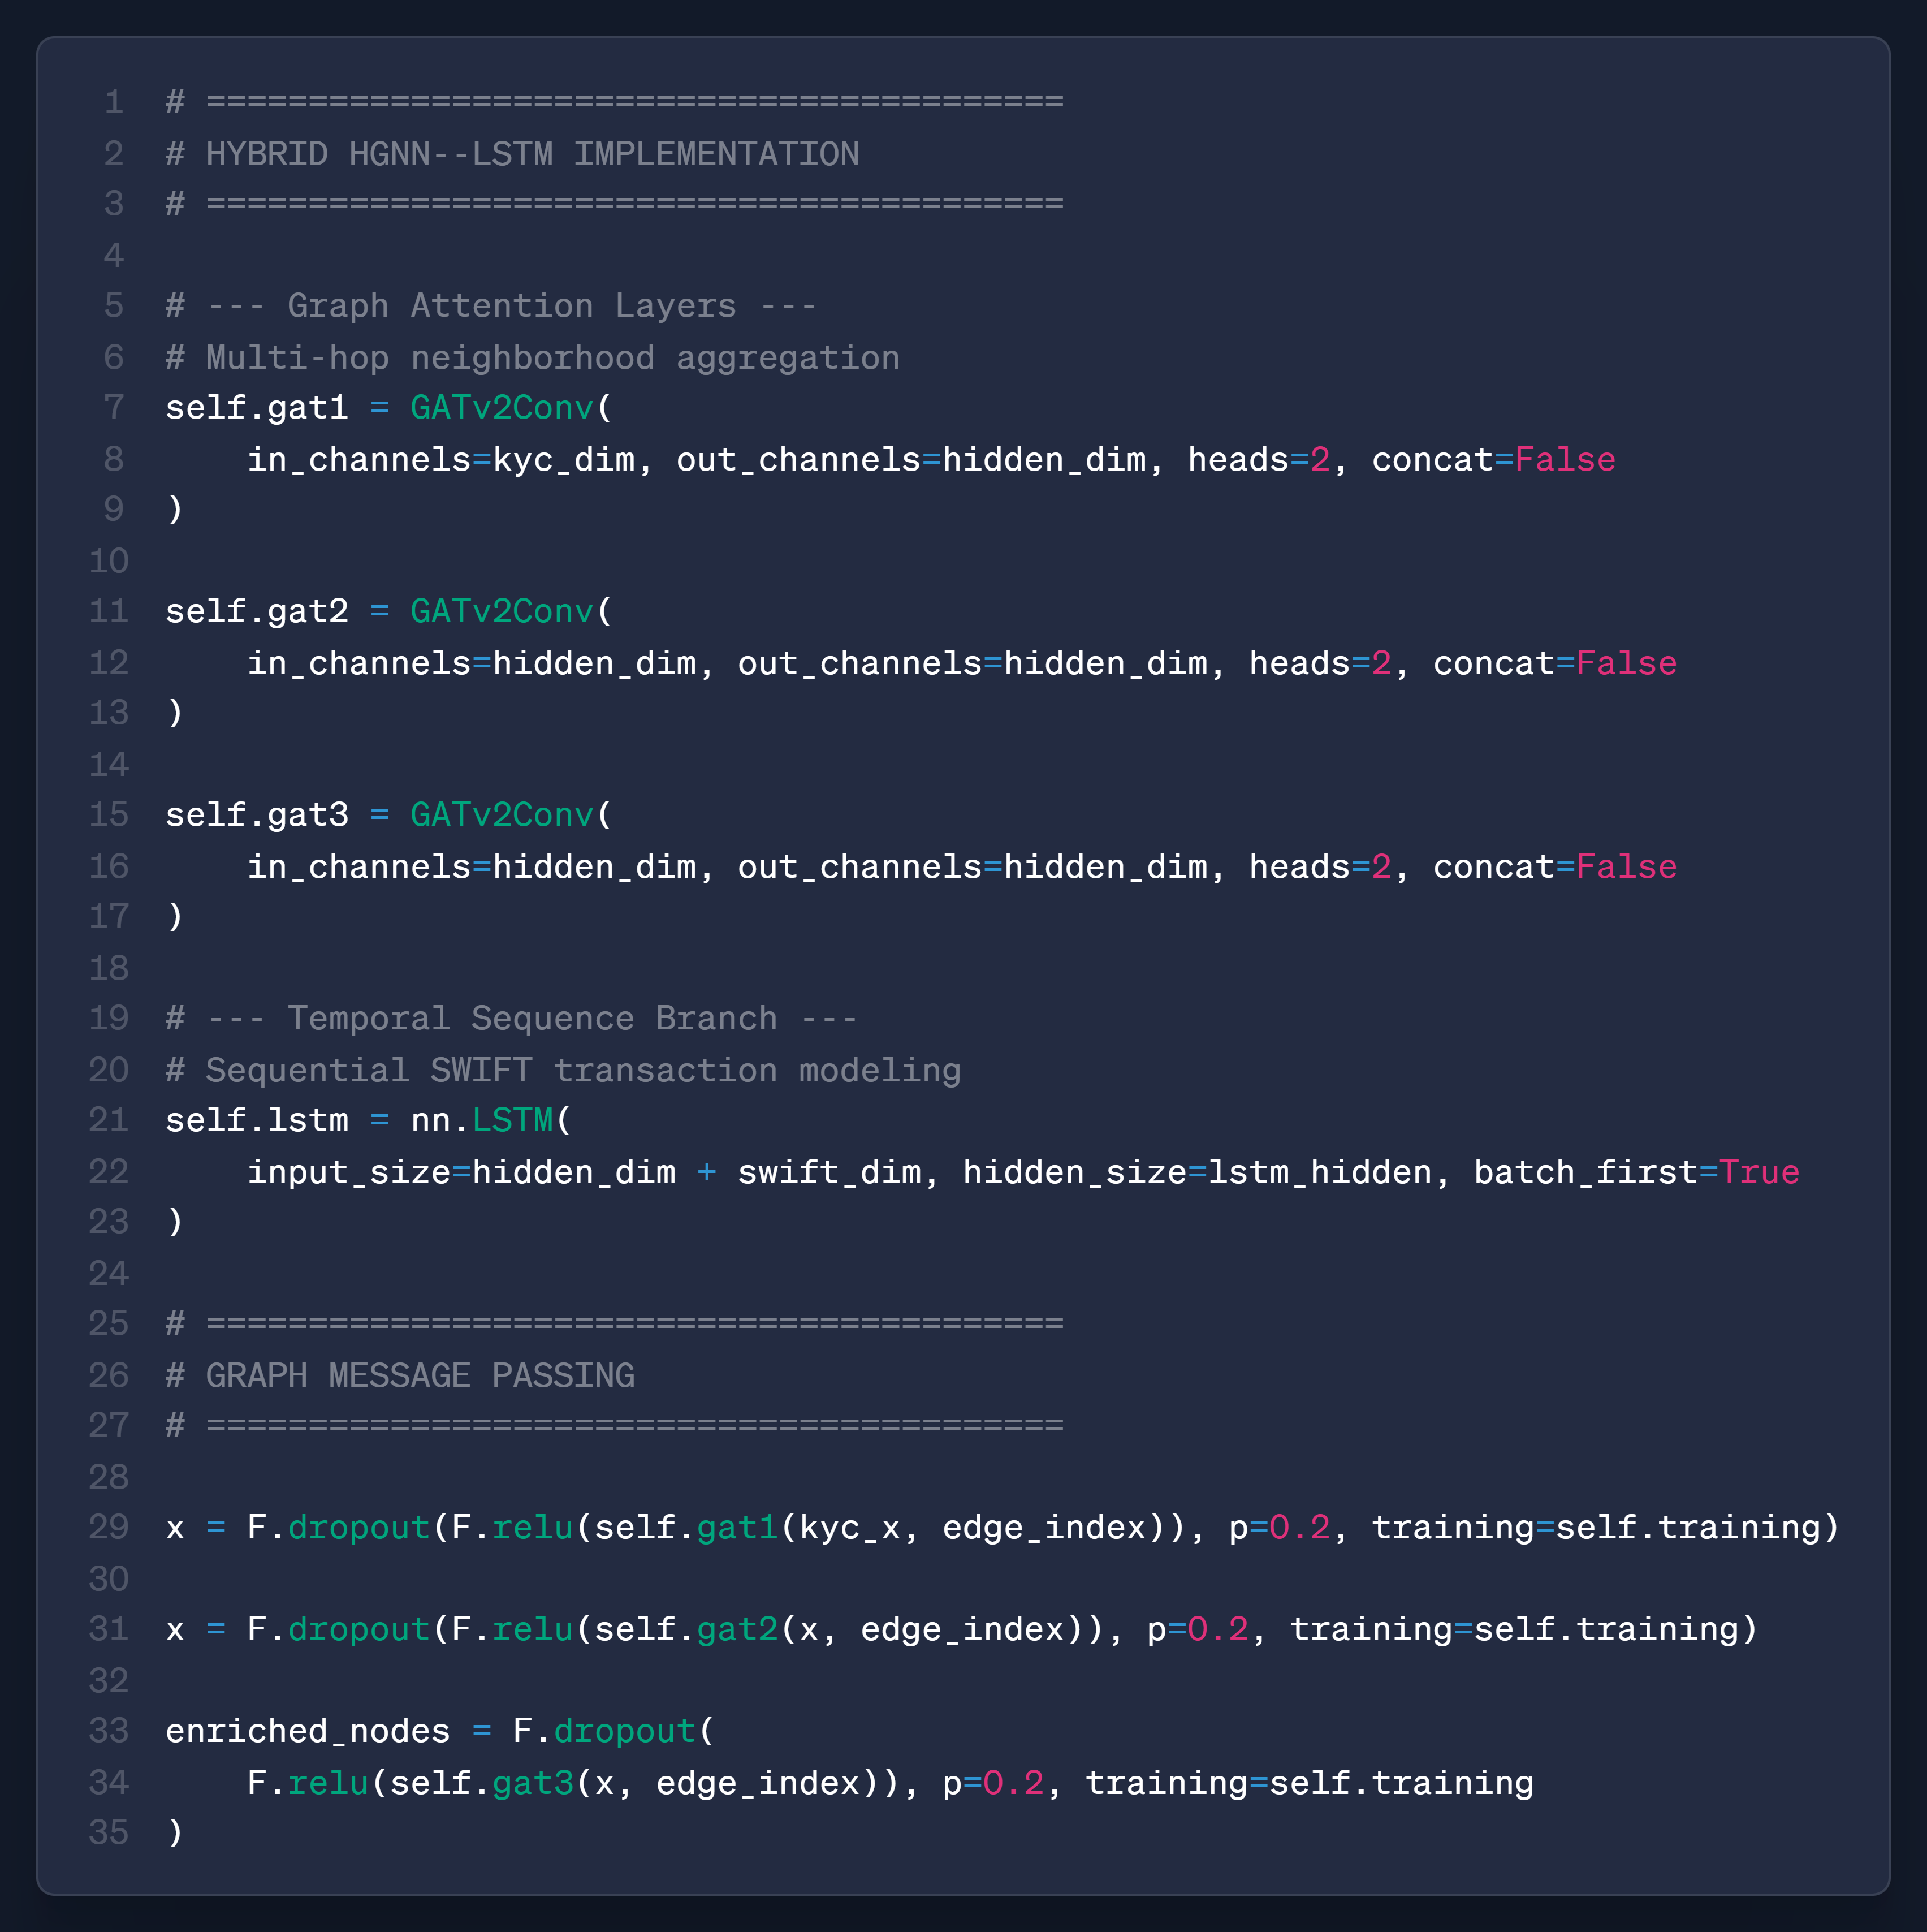
\includegraphics[width=0.48\textwidth]{Figures/model1.png}
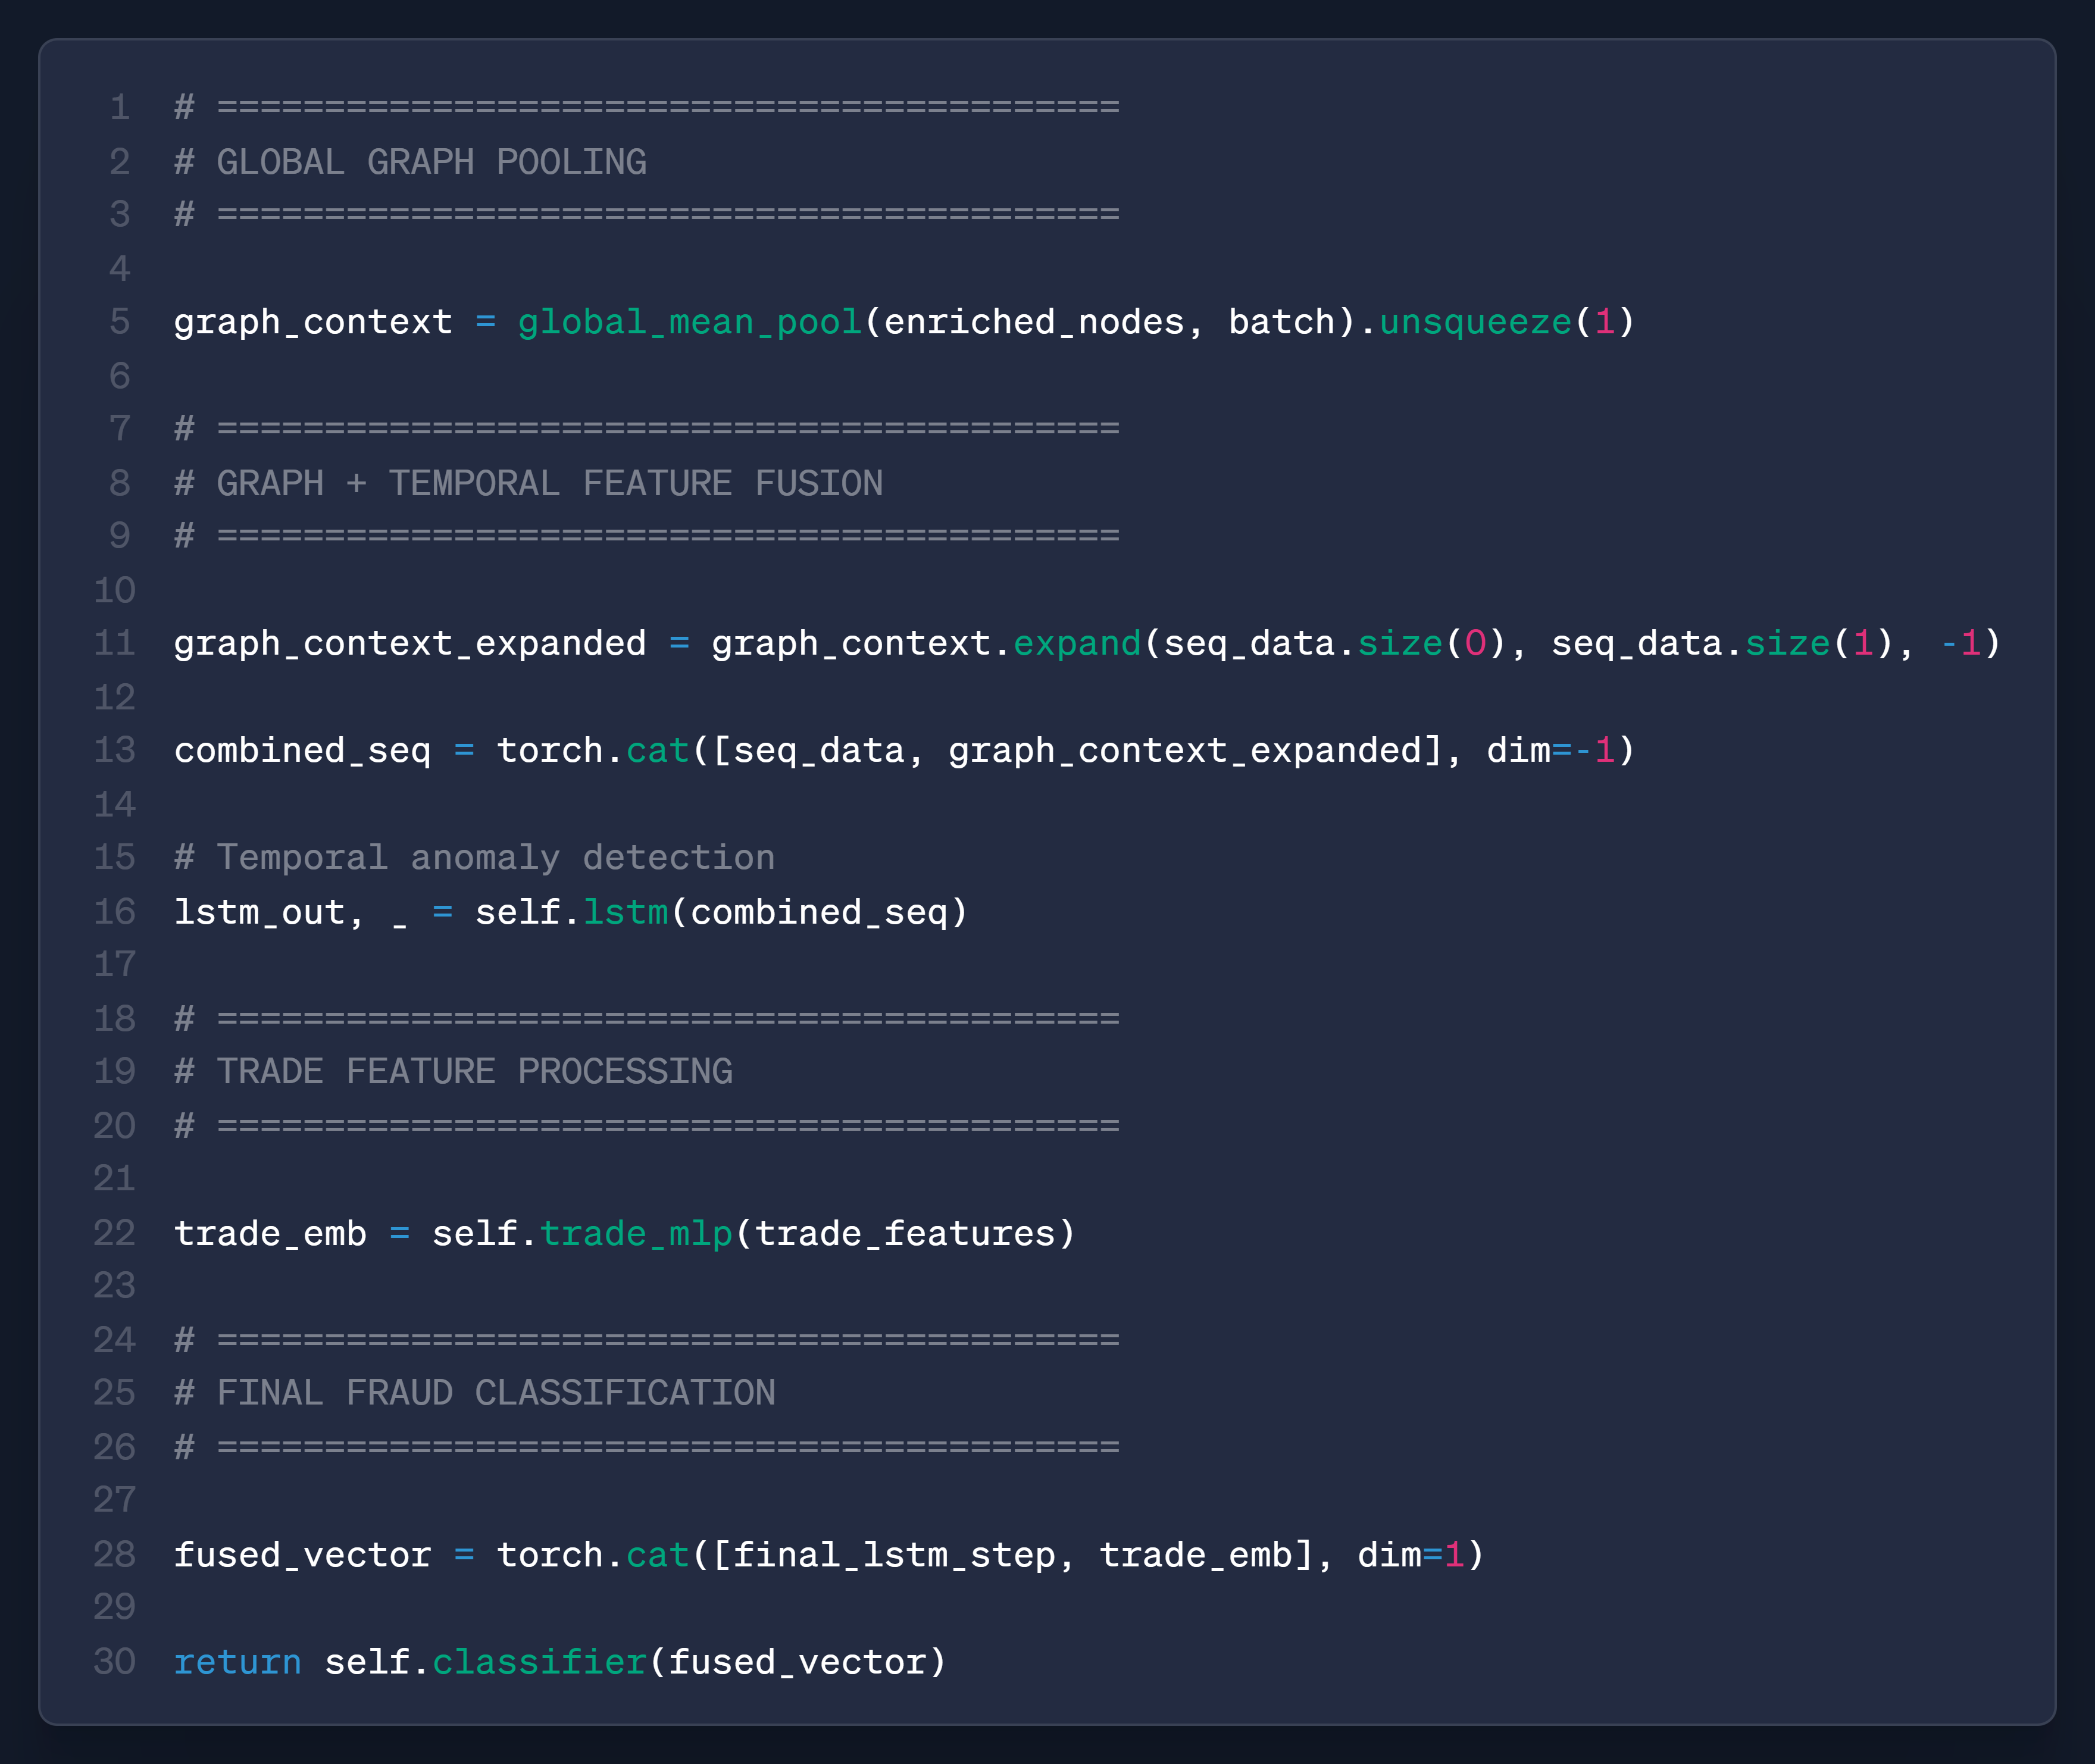
\includegraphics[width=0.48\textwidth]{Figures/model2.png}

\caption{Implementation workflow of the proposed Hybrid HGNN--LSTM analytical module.}

\label{fig:hgnn_impl}

\end{figure}


%========================================================
\subsubsection[Federated Learning Implementation]{\textbf{Federated Learning Implementation}}
%========================================================

The federated learning environment is implemented using the Flower federated learning framework to support distributed privacy-preserving fraud detection across multiple institutional clients. The implementation utilizes a centralized aggregation server and three participating institutional clients, where each client performs localized training of the proposed Hybrid HGNN--LSTM analytical model using institution-specific transaction graphs, sequential SWIFT transaction representations, and fraud classification labels without directly sharing sensitive financial records outside the local analytical environment.

The centralized aggregation server implements a custom federated strategy by extending the \texttt{flwr.server.strategy.FedAvg} class and overriding the \texttt{aggregate\_fit()} operation for distributed parameter aggregation. During each federated communication round, locally trained model weights generated from participating institutional clients are transmitted to the aggregation server where the \texttt{FedAvg} algorithm performs parameter averaging across synchronized client updates to generate a globally optimized fraud detection model. The server initializes the Hybrid HGNN--LSTM analytical architecture using synchronized feature dimensions including three-dimensional KYC node features, one-dimensional SWIFT transaction attributes, two-dimensional trade metadata features, hidden embedding dimensions of size 32, and three-class fraud prediction outputs.

The federated implementation performs ten synchronized communication rounds using complete client participation configurations including \texttt{fraction\_fit=1.0}, \texttt{min\_fit\_clients=3}, and \texttt{min\_available\_clients=3} to maintain stable distributed convergence across institutional environments \cite{kennedy2025federated}. After the final aggregation round, the globally optimized model parameters are converted from Flower parameter streams into NumPy tensors using \texttt{parameters\_to\_ndarrays()} before being serialized and stored as \texttt{global\_model.npz} for downstream real-time fraud inference operations. The implemented federated workflow enabled collaborative fraud learning, stable distributed convergence, and privacy-preserving analytical synchronization while maintaining complete institutional data isolation across participating financial organizations.


%========================================================
\subsection[User Interface and Compliance Workflow Implementation]{\textbf{User Interface and Compliance Workflow Implementation}}
%========================================================

The user interface and compliance-monitoring environment is implemented using Next.js, TypeScript, Tailwind CSS, Prisma ORM, Zustand state management, and PostgreSQL to support secure institutional fraud monitoring and centralized regulatory investigation workflows. The frontend architecture follows a modular service-oriented design consisting of protected dashboard routes, middleware-based authentication guards, API handlers, Prisma-powered database interaction layers, and role-specific monitoring interfaces integrated with the federated analytical inference environment.

%========================================================
\subsubsection[Authentication and Role Validation Pipeline]{\textbf{Authentication and Role Validation Pipeline}}
%========================================================

The authentication workflow is implemented using JWT-based session authorization combined with centralized middleware validation and protected route interception mechanisms. Incoming requests targeting protected dashboard routes are validated through middleware guards where session tokens are verified against predefined authorization scopes including \texttt{BANK\_ADMIN} and \texttt{REGULATOR}. Once validated, the session context is propagated across frontend environments through centralized authentication providers and Zustand-managed session states before protected dashboard components and compliance services are rendered within the client environment.

%========================================================
\subsubsection[Transaction Monitoring and Dashboard Rendering]{\textbf{Transaction Monitoring and Dashboard Rendering}}
%========================================================

Fraud predictions generated by the federated Hybrid HGNN--LSTM inference pipeline are synchronized into centralized PostgreSQL audit tables through backend transaction-processing services. Protected Next.js API handlers subsequently retrieve transaction classifications, fraud scores, STR metadata, and institutional monitoring information using Prisma query operations before dynamically rendering analytical outputs within role-specific dashboard interfaces. The banking administrator dashboard supports transaction filtering, fraud investigation workflows, watchlist escalation procedures, and false-positive reclassification operations through synchronized API-driven transaction state updates across centralized audit environments.

%========================================================
\subsubsection[STR Generation and Notification Workflow]{\textbf{STR Generation and Notification Workflow}}
%========================================================

Transactions classified as fraudulent trigger Suspicious Transaction Report (STR) generation workflows implemented through secured API endpoints and PostgreSQL-backed audit synchronization services. Institutional administrators initiate STR generation requests through protected dashboard interfaces where transaction metadata, fraud classifications, investigation summaries, institutional remarks, and compliance status information are serialized and stored within centralized STR audit tables. The generated STR records are subsequently propagated into regulator-facing monitoring environments through synchronized notification services and backend compliance-routing workflows.

%========================================================
\subsubsection[Regulatory Investigation and Compliance Monitoring]{\textbf{Regulatory Investigation and Compliance Monitoring}}
%========================================================

The regulatory monitoring environment consumes institution-generated STR records, fraud-classified transaction histories, compliance metadata, and supporting analytical evidence through protected API routes and Prisma-based database interaction layers. Regulatory authorities can perform investigation workflows including document-verification requests, institutional inquiry procedures, transaction review operations, and account-freeze initiation requests through centralized compliance interfaces synchronized with backend audit environments. The implemented monitoring workflow supports synchronized fraud prediction, institutional verification, STR lifecycle management, and centralized compliance monitoring within a unified real-time TBML analytical platform.


\section{Testing and Validation}
This section provides a comprehensive overview of the testing and validation processes employed to ensure the correctness, reliability, and performance of the proposed TBML detection framework. It includes descriptions of the testing environment, unit testing strategies for individual components, integration testing for end-to-end workflow validation, performance evaluation under simulated transaction loads, and security assessments to validate access control mechanisms and data protection measures within the framework.

%========================================================
\subsection[Testing Environment]{\textbf{Testing Environment}}
%========================================================

The testing process was conducted in a controlled development environment consisting of Python 3.11, PyTorch, PyTorch Geometric, Apache Kafka, Memgraph, PostgreSQL, and Flower federated learning services operating within isolated virtual environments created using \texttt{venv}. Frontend monitoring interfaces were implemented and validated using Next.js, TypeScript, Tailwind CSS, Prisma ORM, Zustand state management, and JWT-based authentication workflows.

The testing workflow additionally utilized Playwright-based browser automation for validating protected dashboard routes, institutional transaction workflows, STR generation pipelines, and compliance-monitoring interfaces. Database synchronization latency, transaction propagation consistency, backend API communication, and distributed fraud-inference workflows were validated under controlled institutional transaction loads to ensure reliable execution across distributed analytical environments.

%========================================================
\subsection[Unit Testing]{\textbf{Unit Testing}}
%========================================================

Each backend analytical service, dashboard workflow, authentication mechanism, and database synchronization component was independently tested to validate correctness, boundary handling, synchronization stability, and operational consistency before integration into the complete TBML detection framework.
%========================================================
\subsubsection[Unit Testing of Authentication and RBAC Module]{\textbf{Unit Testing of Authentication and RBAC Module}}
%========================================================

The authentication and role-based access control environment was independently validated to ensure secure user authentication, authorization management, middleware-driven route protection, credential verification, and institutional role isolation across banking and regulatory dashboard interfaces. The testing workflow additionally verified protected API access, invalid credential handling, unauthorized route restrictions, and role-specific dashboard rendering across distributed monitoring environments.
\renewcommand{\arraystretch}{1.3}

\begin{table}[H]
\centering
\caption{TC-001: Unit Testing of Authentication and RBAC Module}
\vspace{0.2cm}

\begin{tabular}{|p{4.2cm}|p{9cm}|}
\hline
\textbf{Serial Number of Test Case} & TC-001 \\ \hline
\textbf{Name of Test Case} & Protected Dashboard Access Validation \\ \hline
\textbf{Feature being Tested} & Authentication and Authorization Validation \\ \hline
\textbf{Description} & Validate protected route access, JWT verification, and role-based authorization \\ \hline
\textbf{Sample Input} & Invalid JWT session and unauthorized user request \\ \hline
\textbf{Expected Output} & Unauthorized access denied with authentication error response \\ \hline
\textbf{Actual Output} & Invalid sessions blocked and unauthorized users redirected successfully \\ \hline
\textbf{Remarks} & Successful test \\ \hline
\end{tabular}
\end{table}

Middleware-driven session validation successfully enforced protected route isolation and role-specific dashboard authorization across institutional monitoring environments. The testing workflow validated JWT token verification, session-expiration handling, credential validation, protected API access control, and middleware-based authorization checks across banking and regulator dashboards. Invalid credentials, unauthorized API requests, expired authentication sessions, and direct access attempts to protected routes were correctly rejected using backend access-control policies before protected resources were rendered. The authentication workflow additionally verified successful role mapping for \texttt{BANK\_USER} and  \texttt{ADMIN} entities to ensure secure dashboard isolation and controlled access to institutional fraud-monitoring operations.

%========================================================
\subsubsection[Unit Testing of Kafka Transaction Streaming]{\textbf{Unit Testing of Kafka Transaction Streaming}}
%========================================================

The Kafka transaction streaming environment was independently tested to validate asynchronous transaction publishing, real-time event synchronization, payload integrity validation, and downstream analytical communication across distributed backend services. The testing workflow additionally verified message delivery consistency, topic-based transaction propagation, malformed payload handling, and reliable synchronization between Kafka producer and consumer services operating within the proposed framework.


\begin{table}[H]
\centering
\caption{TC-002: Unit Testing of Kafka Transaction Streaming}
\vspace{0.2cm}

\begin{tabular}{|p{4.2cm}|p{9cm}|}
\hline
\textbf{Serial Number of Test Case} & TC-002 \\ \hline
\textbf{Name of Test Case} & Publish Valid SWIFT Transaction \\ \hline
\textbf{Feature being Tested} & Kafka Event Streaming and Message Synchronization \\ \hline
\textbf{Description} & Validate transaction publishing and topic-based event synchronization \\ \hline
\textbf{Sample Input} & JSON transaction payload containing sender, receiver, amount, and trade metadata \\ \hline
\textbf{Expected Output} & Transaction published into \texttt{incoming\_swift\_messages} topic successfully \\ \hline
\textbf{Actual Output} & Transaction streamed and synchronized successfully across Kafka services \\ \hline
\textbf{Remarks} & Successful test \\ \hline
\end{tabular}
\end{table}

The Kafka streaming module successfully validated asynchronous transaction publishing and backend event synchronization across distributed analytical services. Producer and consumer services maintained reliable message propagation and transaction consistency during continuous event-stream processing operations. Invalid payload structures, malformed transaction metadata, and incomplete financial events were correctly rejected through backend validation workflows before downstream graph-processing and fraud-inference operations were initiated.

%========================================================
\subsubsection[Unit Testing of Graph Construction Module]{\textbf{Unit Testing of Graph Construction Module}}
%========================================================

The heterogeneous graph-construction environment was independently tested to validate transactional node generation, relationship mapping, multi-entity graph synchronization, and Cypher-based ingestion workflows within the Memgraph analytical environment. The testing workflow additionally verified graph consistency, entity-link generation, transaction propagation accuracy, and downstream graph availability for Hybrid HGNN--LSTM analytical inference operations.

\begin{table}[H]
\centering
\caption{TC-003: Unit Testing of Graph Construction Module}
\vspace{0.2cm}

\begin{tabular}{|p{4.2cm}|p{9cm}|}
\hline
\textbf{Serial Number of Test Case} & TC-003 \\ \hline
\textbf{Name of Test Case} & Heterogeneous Graph Entity Generation \\ \hline
\textbf{Feature being Tested} & Memgraph Graph Construction and Relationship Mapping \\ \hline
\textbf{Description} & Validate transactional node generation and graph relationship synchronization \\ \hline
\textbf{Sample Input} & Valid SWIFT transaction payload with account, trade, and document metadata \\ \hline
\textbf{Expected Output} & Graph nodes and transactional relationships created successfully within Memgraph \\ \hline
\textbf{Actual Output} & Heterogeneous graph entities and multi-hop relationships generated successfully \\ \hline
\textbf{Remarks} & Successful test \\ \hline
\end{tabular}
\end{table}

The graph-construction workflow successfully generated heterogeneous transactional graphs within the Memgraph environment using Cypher-based ingestion and relationship-mapping operations. Graph entities including \texttt{(:Account)}, \texttt{(:Transaction)}, and \texttt{(:Document)} were correctly synchronized with transactional relationships such as \texttt{[:SENDS]}, \texttt{[:TO]}, and \texttt{[:HAS\_DOC]} during continuous event-stream processing. The testing workflow additionally validated graph consistency, entity-link integrity, and multi-hop transactional connectivity required for downstream subgraph extraction and graph-based fraud inference operations within the proposed framework.

%========================================================
\subsubsection[Unit Testing of STR Generation Workflow]{\textbf{Unit Testing of STR Generation Workflow}}
%========================================================

The STR generation workflow was independently tested to validate suspicious transaction report generation, compliance-record synchronization, fraud-case escalation, and regulator-side notification propagation across distributed institutional monitoring environments. The testing workflow additionally verified report persistence, transaction-metadata preservation, audit consistency, and downstream synchronization between banking dashboards and regulator-facing compliance interfaces.


\begin{table}[H]
\centering
\caption{TC-004: Unit Testing of STR Generation Workflow}
\vspace{0.2cm}

\begin{tabular}{|p{4.2cm}|p{9cm}|}
\hline
\textbf{Serial Number of Test Case} & TC-004 \\ \hline
\textbf{Name of Test Case} & Suspicious Transaction Report Generation \\ \hline
\textbf{Feature being Tested} & STR Generation and Compliance Synchronization \\ \hline
\textbf{Description} & Validate fraud escalation and regulator-side STR synchronization workflow \\ \hline
\textbf{Sample Input} & Fraud-classified transaction selected from institutional monitoring dashboard \\ \hline
\textbf{Expected Output} & STR record generated and synchronized into regulator compliance environment \\ \hline
\textbf{Actual Output} & STR generated, persisted, and synchronized successfully across monitoring services \\ \hline
\textbf{Remarks} & Successful test \\ \hline
\end{tabular}
\end{table}


The STR workflow successfully validated automated fraud-report generation, PostgreSQL audit synchronization, and regulator-side notification propagation across distributed institutional environments. Generated STR records correctly preserved transaction metadata, fraud classifications, institutional identifiers, and investigation references during downstream compliance synchronization operations. The testing workflow additionally verified successful dashboard synchronization, report persistence, and controlled propagation of suspicious transaction alerts between banking institutions and regulatory monitoring interfaces operating within the proposed framework.

%========================================================
\subsubsection[Unit Testing of Notification Workflow]{\textbf{Unit Testing of Notification Workflow}}
%========================================================

The notification synchronization environment was independently tested to validate fraud-alert propagation, institutional notification delivery, compliance-event synchronization, and regulator-side alert visibility across distributed monitoring interfaces. The testing workflow additionally verified notification persistence, dashboard update consistency, backend event propagation, and synchronization between banking and regulatory compliance environments during fraud escalation operations.


\begin{table}[H]
\centering
\caption{TC-005: Unit Testing of Notification Workflow}
\vspace{0.2cm}

\begin{tabular}{|p{4.2cm}|p{9cm}|}
\hline
\textbf{Serial Number of Test Case} & TC-005 \\ \hline
\textbf{Name of Test Case} & Fraud Alert and Compliance Notification Propagation \\ \hline
\textbf{Feature being Tested} & Notification Synchronization and Alert Delivery \\ \hline
\textbf{Description} & Validate fraud-alert propagation across banking and regulator monitoring environments \\ \hline
\textbf{Sample Input} & Generated STR record linked to fraud-classified transaction \\ \hline
\textbf{Expected Output} & Compliance alerts synchronized into regulator-facing dashboard interfaces \\ \hline
\textbf{Actual Output} & Fraud notifications propagated and synchronized successfully \\ \hline
\textbf{Remarks} & Successful test \\ \hline
\end{tabular}
\end{table}


The notification workflow successfully validated fraud-alert propagation, institutional investigation updates, and STR lifecycle synchronization across distributed compliance-monitoring environments. Backend event-processing services maintained reliable notification delivery and dashboard synchronization during fraud escalation operations between banking institutions and regulatory authorities. The testing workflow additionally verified notification persistence, regulator-side alert visibility, and consistent compliance-state propagation across protected monitoring interfaces operating within the proposed framework.



%========================================================
\subsection[Integration Testing]{\textbf{Integration Testing}}
%========================================================

Integration testing was conducted to validate the interaction, synchronization consistency, and workflow stability between distributed analytical services, graph-processing environments, fraud inference pipelines, dashboard-rendering systems, and regulatory compliance workflows operating within the proposed TBML detection framework.

%========================================================
\subsubsection[Integration Testing of Kafka and Memgraph Pipeline]{\textbf{Integration Testing of Kafka and Memgraph Pipeline}}
%========================================================

This integration test validated end-to-end synchronization between Kafka-based transaction streaming services and the heterogeneous graph-construction environment operating within Memgraph. The testing workflow additionally verified event-stream consistency, transaction propagation reliability, graph-ingestion stability, and downstream synchronization between distributed backend services.

\renewcommand{\arraystretch}{1.3}

\begin{table}[H]
\centering
\caption{TC-006: Integration Testing of Kafka and Memgraph Pipeline}
\vspace{0.2cm}

\begin{tabular}{|p{4.2cm}|p{9cm}|}
\hline
\textbf{Serial Number of Test Case} & TC-006 \\ \hline
\textbf{Name of Test Case} & Transaction Stream and Graph Synchronization Workflow \\ \hline
\textbf{Feature being Tested} & Kafka Event Propagation and Memgraph Synchronization \\ \hline
\textbf{Description} & Validate transaction-stream synchronization and heterogeneous graph generation \\ \hline
\textbf{Sample Input} & Valid Kafka transaction payload with trade metadata and KYC attributes \\ \hline
\textbf{Expected Output} & Transactional graph entities and relationships generated successfully within Memgraph \\ \hline
\textbf{Actual Output} & Kafka events synchronized and heterogeneous graph generated successfully \\ \hline
\textbf{Remarks} & Successful test \\ \hline
\end{tabular}
\end{table}

\renewcommand{\arraystretch}{1}

The integration workflow successfully validated asynchronous transaction propagation between Kafka producer-consumer services and Memgraph graph-ingestion environments. Streamed SWIFT transaction events were reliably synchronized into graph-processing pipelines without transactional inconsistency or event-loss during continuous backend processing operations. The testing workflow additionally verified stable graph synchronization, multi-entity relationship generation, and downstream availability of transactional subgraphs required for graph-based analytical inference within the proposed framework.


%========================================================
\subsubsection[Integration Testing of Fraud Prediction and Dashboard Synchronization]{\textbf{Integration Testing of Fraud Prediction and Dashboard Synchronization}}
%========================================================

This integration test checked how well the fraud-prediction services, PostgreSQL audit layer, and role-based monitoring dashboards worked together within the proposed TBML framework. It also confirmed that transaction results were stored correctly, updated reliably on the dashboard, and rendered in real time for fraud-monitoring review.

\renewcommand{\arraystretch}{1.3}

\begin{table}[H]
\centering
\caption{TC-007: Integration Testing of Fraud Prediction and Dashboard Synchronization}
\vspace{0.2cm}

\begin{tabular}{|p{4.2cm}|p{9cm}|}
\hline
\textbf{Serial Number of Test Case} & TC-007 \\ \hline
\textbf{Name of Test Case} & Fraud Prediction and Dashboard Rendering Workflow \\ \hline
\textbf{Feature being Tested} & PostgreSQL Synchronization and Dashboard Visualization \\ \hline
\textbf{Description} & Validate fraud-prediction synchronization into institutional monitoring dashboards \\ \hline
\textbf{Sample Input} & Fraud-classified transaction generated from analytical inference pipeline \\ \hline
\textbf{Expected Output} & Fraud transaction persisted and rendered successfully within dashboard interfaces \\ \hline
\textbf{Actual Output} & Dashboard synchronization completed successfully with valid fraud-state rendering \\ \hline
\textbf{Remarks} & Successful test \\ \hline
\end{tabular}
\end{table}

\renewcommand{\arraystretch}{1}

Fraud-prediction records, transaction metadata, and institutional risk classifications were synced into the central PostgreSQL audit environment and then displayed through protected dashboard interfaces. The dashboard updates stayed consistent across institutional monitoring services, giving users a clear real-time view of transaction status and fraud outcomes. The test also confirmed stable backend persistence, reliable dashboard refreshes, and secure rendering of fraud-monitoring data for each role-based compliance environment.

%========================================================
\subsubsection[Integration Testing of STR Generation Workflow]{\textbf{Integration Testing of STR Generation Workflow}}
%========================================================

This integration test covered the full path from institutional fraud review to STR generation, regulator synchronization, and compliance notifications across distributed monitoring environments. It verified that fraud escalation behaved consistently, reports were stored correctly, and regulators could see the same case information across their compliance pipelines.

The STR workflow worked as expected: once a transaction was marked for escalation, the system generated the compliance report, synchronized it to the regulator-side dashboard, and propagated the related notifications across the monitoring environment. Each STR record retained the key fraud classification details, investigation notes, institutional identifiers, and audit references needed for downstream compliance processing. The test also confirmed that compliance alerts reached the relevant banking and regulatory interfaces in a synchronized way.

\renewcommand{\arraystretch}{1.3}

\begin{table}[H]
\centering
\caption{TC-008: Integration Testing of STR Generation Workflow}
\vspace{0.2cm}

\begin{tabular}{|p{4.2cm}|p{9cm}|}
\hline
\textbf{Serial Number of Test Case} & TC-008 \\ \hline
\textbf{Name of Test Case} & Fraud Escalation and STR Compliance Workflow \\ \hline
\textbf{Feature being Tested} & STR Lifecycle Management and Compliance Synchronization \\ \hline
\textbf{Description} & Validate fraud escalation and regulator-side STR synchronization workflow \\ \hline
\textbf{Sample Input} & Fraud transaction escalated by institutional administrator \\ \hline
\textbf{Expected Output} & STR generated and synchronized successfully within regulator compliance dashboard \\ \hline
\textbf{Actual Output} & Fraud escalation and STR synchronization completed successfully \\ \hline
\textbf{Remarks} & Successful test \\ \hline
\end{tabular}
\end{table}

\renewcommand{\arraystretch}{1}


%========================================================
\subsubsection[Integration Testing of Authentication and Protected Dashboard Rendering]{\textbf{Integration Testing of Authentication and Protected Dashboard Rendering}}
%========================================================

This integration test validated synchronization between JWT-based authentication services, middleware-driven authorization guards, protected API routes, and role-specific dashboard-rendering environments operating within the proposed framework. The testing workflow additionally verified secure session propagation, authorization consistency, and protected resource accessibility across institutional monitoring interfaces.

Middleware-driven authentication workflows successfully validated session authorization, protected route synchronization, secure API accessibility, and institutional role isolation across distributed monitoring interfaces. Dashboard-rendering operations correctly enforced role-specific access-control policies for \texttt{BANK\_USER}, \texttt{ADMIN}, and \texttt{REGULATOR} entities during backend synchronization workflows. The testing workflow additionally verified invalid-session rejection, unauthorized route restrictions, and secure propagation of authenticated dashboard resources across institutional compliance-monitoring environments.
\renewcommand{\arraystretch}{1.3}

\begin{table}[H]
\centering
\caption{TC-009: Integration Testing of Authentication and Protected Dashboard Rendering}
\vspace{0.2cm}

\begin{tabular}{|p{4.2cm}|p{9cm}|}
\hline
\textbf{Serial Number of Test Case} & TC-009 \\ \hline
\textbf{Name of Test Case} & Authenticated Dashboard Access and Rendering Workflow \\ \hline
\textbf{Feature being Tested} & Session Validation and Role-Based Dashboard Authorization \\ \hline
\textbf{Description} & Validate authenticated dashboard rendering and protected route authorization \\ \hline
\textbf{Sample Input} & Valid JWT-authenticated institutional user session \\ \hline
\textbf{Expected Output} & Authorized dashboard rendered successfully based on institutional role \\ \hline
\textbf{Actual Output} & Protected dashboard rendered successfully with valid role authorization \\ \hline
\textbf{Remarks} & Successful test \\ \hline
\end{tabular}
\end{table}

\renewcommand{\arraystretch}{1}

%========================================================
\subsection[System Testing]{\textbf{System Testing}}
%========================================================

System testing was used to check how the proposed TBML detection framework behaved under realistic operational load. The focus was on end-to-end browser validation, protected dashboard execution, concurrent PostgreSQL access, API response times, and latency behavior across the fraud-monitoring and compliance-management services. The goal was to confirm that the system remained stable, responsive, and consistent when several components were active at the same time in a distributed institutional setting.

%========================================================
\subsubsection[Browser Automation and Workflow Validation]{\textbf{Browser Automation and Workflow Validation}}
%========================================================

Browser-based end-to-end validation was performed using Playwright automation workflows executed within Chromium testing environments. The testing workflow validated protected dashboard rendering, role-based authentication, STR lifecycle execution, fraud-notification propagation, compliance-action synchronization, and institutional transaction visibility restrictions across distributed frontend and backend services. All automated workflow executions completed successfully without unauthorized access, synchronization failure, or dashboard inconsistency during operational validation.

\renewcommand{\arraystretch}{1.3}

\begin{table}[H]
\centering
\caption{TC-010: Browser Automation and Workflow Validation Results}
\vspace{0.2cm}

\begin{tabular}{|p{7cm}|p{4cm}|}
\hline
\textbf{Workflow Validation} & \textbf{Status} \\ \hline
Admin Authentication and Dashboard Rendering & Successful \\ \hline
Fraud Case Retrieval and STR Visibility & Successful \\ \hline
GET\_DOCUMENTS Compliance Workflow & Successful \\ \hline
FREEZE\_ACCOUNT Regulatory Workflow & Successful \\ \hline
Fraud Verdict Marking Workflow & Successful \\ \hline
Bank User STR Generation Workflow & Successful \\ \hline
Fraud Notification Propagation Workflow & Successful \\ \hline
Protected Route and RBAC Validation & Successful \\ \hline
Institutional Transaction Visibility Restriction & Successful \\ \hline
Sign-In Page Smoke Testing & Successful \\ \hline
\end{tabular}
\end{table}

\renewcommand{\arraystretch}{1}

The Playwright automation workflow confirmed that institutional fraud-monitoring actions could be carried out in sequence across protected dashboard environments without interruption. It also verified secure session persistence, consistent API synchronization, proper workflow-level authorization, and stable dashboard rendering for both \texttt{ADMIN} and \texttt{BANK\_USER} users. In addition, the test showed that STR generation, fraud escalation, regulator-side compliance synchronization, and notification propagation all worked correctly in the automated end-to-end workflow.

%========================================================
\subsubsection[Concurrent Database Scalability and API Performance Analysis]{\textbf{Concurrent Database Scalability and API Performance Analysis}}
%========================================================

Concurrent database scalability testing assessed how well PostgreSQL synchronization held up under increasing institutional user loads, along with dashboard query performance, fraud-filtering latency, and STR retrieval consistency. The benchmark used Prisma ORM and Next.js backend services, and each simulated user sent five continuous transactional requests while accessing the dashboard. To keep the workload stable, the test used batched asynchronous requests, pooled PostgreSQL connections, and a limit of 15 active connections so that synchronization stayed reliable and backend resources were not overloaded during heavy monitoring activity.

Latency benchmarking was carried out by recording request-start and response-finish timestamps during concurrent API execution. For each request, the workflow captured the start time using \texttt{startTime = performance.now()}, sent the asynchronous API call, and then recorded the end time using \texttt{endTime = performance.now()} once the response returned. The latency was calculated as \texttt{latency = endTime - startTime}. The workload was run in parallel so that multiple simulated institutional users could issue dashboard and compliance queries at the same time under controlled concurrency limits.

Average latency reflected the mean response time across all successful requests, while P95 latency captured the slower end of the response distribution for 95\% of requests during peak load. The benchmark also checked request throughput, API synchronization consistency, transaction persistence reliability, and stable PostgreSQL query execution across distributed compliance-monitoring environments.

The benchmarking metrics were computed using the following operational latency equations:

\begin{equation}
L_{\text{avg}} =
\frac{1}{N}
\sum_{i=1}^{N}
(T_{\text{response}_i} - T_{\text{request}_i})
\end{equation}

\begin{equation}
L_{95} =
\operatorname{Percentile}_{95}(L_1, L_2, \dots, L_N)
\end{equation}

\renewcommand{\arraystretch}{1.3}

\begin{table}[H]
\centering
\caption{TC-011: Dashboard Transaction Retrieval Scalability Analysis}
\vspace{0.2cm}

\begin{tabular}{|p{2.6cm}|p{2.4cm}|p{2.8cm}|p{2.8cm}|p{2.2cm}|}
\hline
\textbf{Concurrent Users} & \textbf{Total Requests} & \textbf{Avg Latency (ms)} & \textbf{P95 Latency (ms)} & \textbf{Success Rate} \\ \hline
10 & 50 & 297.33 & 884.28 & 100\% \\ \hline
50 & 250 & 156.05 & 174.75 & 100\% \\ \hline
100 & 500 & 159.99 & 181.30 & 100\% \\ \hline
250 & 1250 & 158.53 & 176.99 & 100\% \\ \hline
500 & 2500 & 162.14 & 180.72 & 100\% \\ \hline
\end{tabular}
\end{table}

\renewcommand{\arraystretch}{1}

The dashboard transaction retrieval workflow demonstrated stable query scalability and consistent dashboard-rendering performance across increasing institutional user loads. Average latency values remained nearly constant between 50 and 500 concurrent users, indicating efficient PostgreSQL query execution, optimized transactional indexing, and stable backend synchronization during high-frequency dashboard-access operations. The relatively low variation between average and P95 latency measurements further indicated predictable response behavior and controlled query-execution overhead under concurrent transactional workloads.

\renewcommand{\arraystretch}{1.3}

\begin{table}[H]
\centering
\caption{TC-012: Fraud Transaction Filtering Scalability Analysis}
\vspace{0.2cm}

\begin{tabular}{|p{2.6cm}|p{2.4cm}|p{2.8cm}|p{2.8cm}|p{2.2cm}|}
\hline
\textbf{Concurrent Users} & \textbf{Total Requests} & \textbf{Avg Latency (ms)} & \textbf{P95 Latency (ms)} & \textbf{Success Rate} \\ \hline
10 & 50 & 159.58 & 174.04 & 100\% \\ \hline
50 & 250 & 158.15 & 181.58 & 100\% \\ \hline
100 & 500 & 147.56 & 170.37 & 100\% \\ \hline
250 & 1250 & 148.18 & 164.58 & 100\% \\ \hline
500 & 2500 & 263.80 & 731.88 & 100\% \\ \hline
\end{tabular}
\end{table}

\renewcommand{\arraystretch}{1}

The fraud-transaction filtering workflow demonstrated efficient analytical-query execution and stable institution-specific transaction retrieval during concurrent dashboard operations. Lower average latency values under moderate workloads indicated optimized fraud-state filtering and indexed transactional query execution across backend analytical services. Increased P95 latency under 500-user workloads indicated temporary synchronization overhead during peak concurrent analytical filtering operations; however, the framework maintained complete request reliability, stable API synchronization, and consistent fraud-state propagation throughout distributed monitoring workflows.

\renewcommand{\arraystretch}{1.3}

\begin{table}[H]
\centering
\caption{TC-013: STR Compliance Report Retrieval Scalability Analysis}
\vspace{0.2cm}

\begin{tabular}{|p{2.6cm}|p{2.4cm}|p{2.8cm}|p{2.8cm}|p{2.2cm}|}
\hline
\textbf{Concurrent Users} & \textbf{Total Requests} & \textbf{Avg Latency (ms)} & \textbf{P95 Latency (ms)} & \textbf{Success Rate} \\ \hline
10 & 50 & 2694.21 & 7311.50 & 100\% \\ \hline
50 & 250 & 2101.61 & 4791.52 & 100\% \\ \hline
100 & 500 & 856.39 & 2149.27 & 100\% \\ \hline
250 & 1250 & 467.03 & 600.67 & 100\% \\ \hline
500 & 2500 & 465.62 & 596.76 & 100\% \\ \hline
\end{tabular}
\end{table}

\renewcommand{\arraystretch}{1}

The STR compliance retrieval workflow showed higher latency than the other dashboard operations because it had to aggregate compliance reports, synchronize transaction history, retrieve regulator-side metadata, and execute several relational queries during report generation. Even so, the drop in average latency as concurrency increased suggested that PostgreSQL query handling became more stable, pooled connections were used more efficiently, and relational queries were executed more smoothly during sustained processing.

Although compliance-report generation added extra processing overhead, the framework still maintained consistent request behavior and a complete success rate across distributed monitoring environments. Overall, the testing workflows showed reliable backend synchronization, controlled API responses, stable federated analytical execution, and steady PostgreSQL performance as institutional workload increased.


Taken together, the testing results confirmed that the proposed TBML detection framework remained reliable, stable, and consistent across graph-processing, federated inference, dashboard synchronization, and compliance-management services. The scalability results also showed that PostgreSQL execution stayed stable and latency remained controlled even as institutional traffic increased.



%========================================================
\subsection[Model Performance Evaluation]{\textbf{Model Performance Evaluation}}
%========================================================

The proposed federated Hybrid HGNN--LSTM framework was evaluated across three distributed institutional clients (BANKA, BANKB, and BANKC) to validate fraud-classification capability and federated convergence stability across heterogeneous transactional environments. Multi-class prediction performance for \textit{Clean}, \textit{Watchlist}, and \textit{Fraud} transaction states was analyzed using Precision, Recall, F1-Score, confusion-matrix validation, and Precision--Recall benchmarking. Federated parameter synchronization was performed using the FedAvg aggregation strategy across 10 federated communication rounds.

The transactional dataset was partitioned using a stratified temporal split strategy to preserve chronological separation between training and testing samples while maintaining balanced representation across minority fraud categories. Weighted cross-entropy optimization and gradient clipping mechanisms were integrated to stabilize distributed training and address fraud-class imbalance during federated convergence operations. Precision--Recall evaluation was prioritized over standalone classification accuracy due to the highly imbalanced nature of illicit transactional behavior within institutional financial environments.

%========================================================
\subsubsection[Multi-Class Classification Performance]{\textbf{Multi-Class Classification Performance}}
%========================================================

The final federated classification results obtained after 10 federated aggregation rounds across all participating institutional environments are summarized in Table~\ref{tab:model_performance}. The evaluation was conducted to analyze the framework’s ability to distinguish legitimate, suspicious, and fraudulent transactional behaviors across distributed institutional datasets under federated learning conditions. The obtained results additionally validated stable analytical convergence and consistent fraud-classification performance across all participating banking clients.


The results showed that the model classified the three transaction states consistently across all institutional clients. Clean transactions were identified with near-perfect Precision and Recall, which helped keep false positives low during large-scale monitoring. The Watchlist class also performed well, with Recall remaining above $0.97$, showing that the model could reliably flag suspicious activity for institutional review.

\begin{table}[H]
\centering
\caption{Federated Multi-Class Classification Performance result}
\vspace{0.2cm}

\renewcommand{\arraystretch}{1.3}

\begin{tabular}{|p{2.2cm}|p{3cm}|p{2cm}|p{2cm}|p{2cm}|}
\hline
\textbf{Institution} & \textbf{Transaction Class} & \textbf{Precision} & \textbf{Recall} & \textbf{F1-Score} \\ \hline

\multirow{3}{*}{BANKA}
& Clean (0) & 1.00 & 1.00 & 1.00 \\ \cline{2-5}
& Watchlist (1) & 0.79 & 0.97 & 0.87 \\ \cline{2-5}
& Fraud (2) & 0.96 & 0.73 & 0.83 \\ \hline

\multirow{3}{*}{BANKB}
& Clean (0) & 1.00 & 1.00 & 1.00 \\ \cline{2-5}
& Watchlist (1) & 0.79 & 0.99 & 0.88 \\ \cline{2-5}
& Fraud (2) & 0.98 & 0.73 & 0.84 \\ \hline

\multirow{3}{*}{BANKC}
& Clean (0) & 1.00 & 1.00 & 1.00 \\ \cline{2-5}
& Watchlist (1) & 0.79 & 0.99 & 0.88 \\ \cline{2-5}
& Fraud (2) & 0.98 & 0.73 & 0.84 \\ \hline

\end{tabular}

\renewcommand{\arraystretch}{1}

\label{tab:model_performance}
\end{table}


Fraud-class predictions achieved Precision values between $0.96$ and $0.98$, which indicates that high-risk transactions were identified with very few false fraud alerts. Fraud Recall stayed around $0.73$, but the framework still preserved strong fraud-detection capability even with highly imbalanced data and complex multi-hop laundering structures. Overall, the results showed that the federated model generalized well across distributed institutions without requiring sensitive data to be centralized.


%========================================================
\subsubsection[Federated Convergence Analysis]{\textbf{Federated Convergence Analysis}}
%========================================================

Federated convergence was evaluated by tracking Accuracy, Precision, and Recall across successive aggregation rounds. Separate curves were generated for BANKA, BANKB, and BANKC so that the synchronization behavior of each institutional client could be observed independently. This made it possible to confirm that local updates were being aggregated correctly and that the global model was stabilizing as training progressed.

%--------------------------------------------------------
\subsubsection{BANKA Federated Convergence}
%--------------------------------------------------------

\begin{figure}[H]
\centering

\begin{minipage}{0.32\textwidth}
\centering
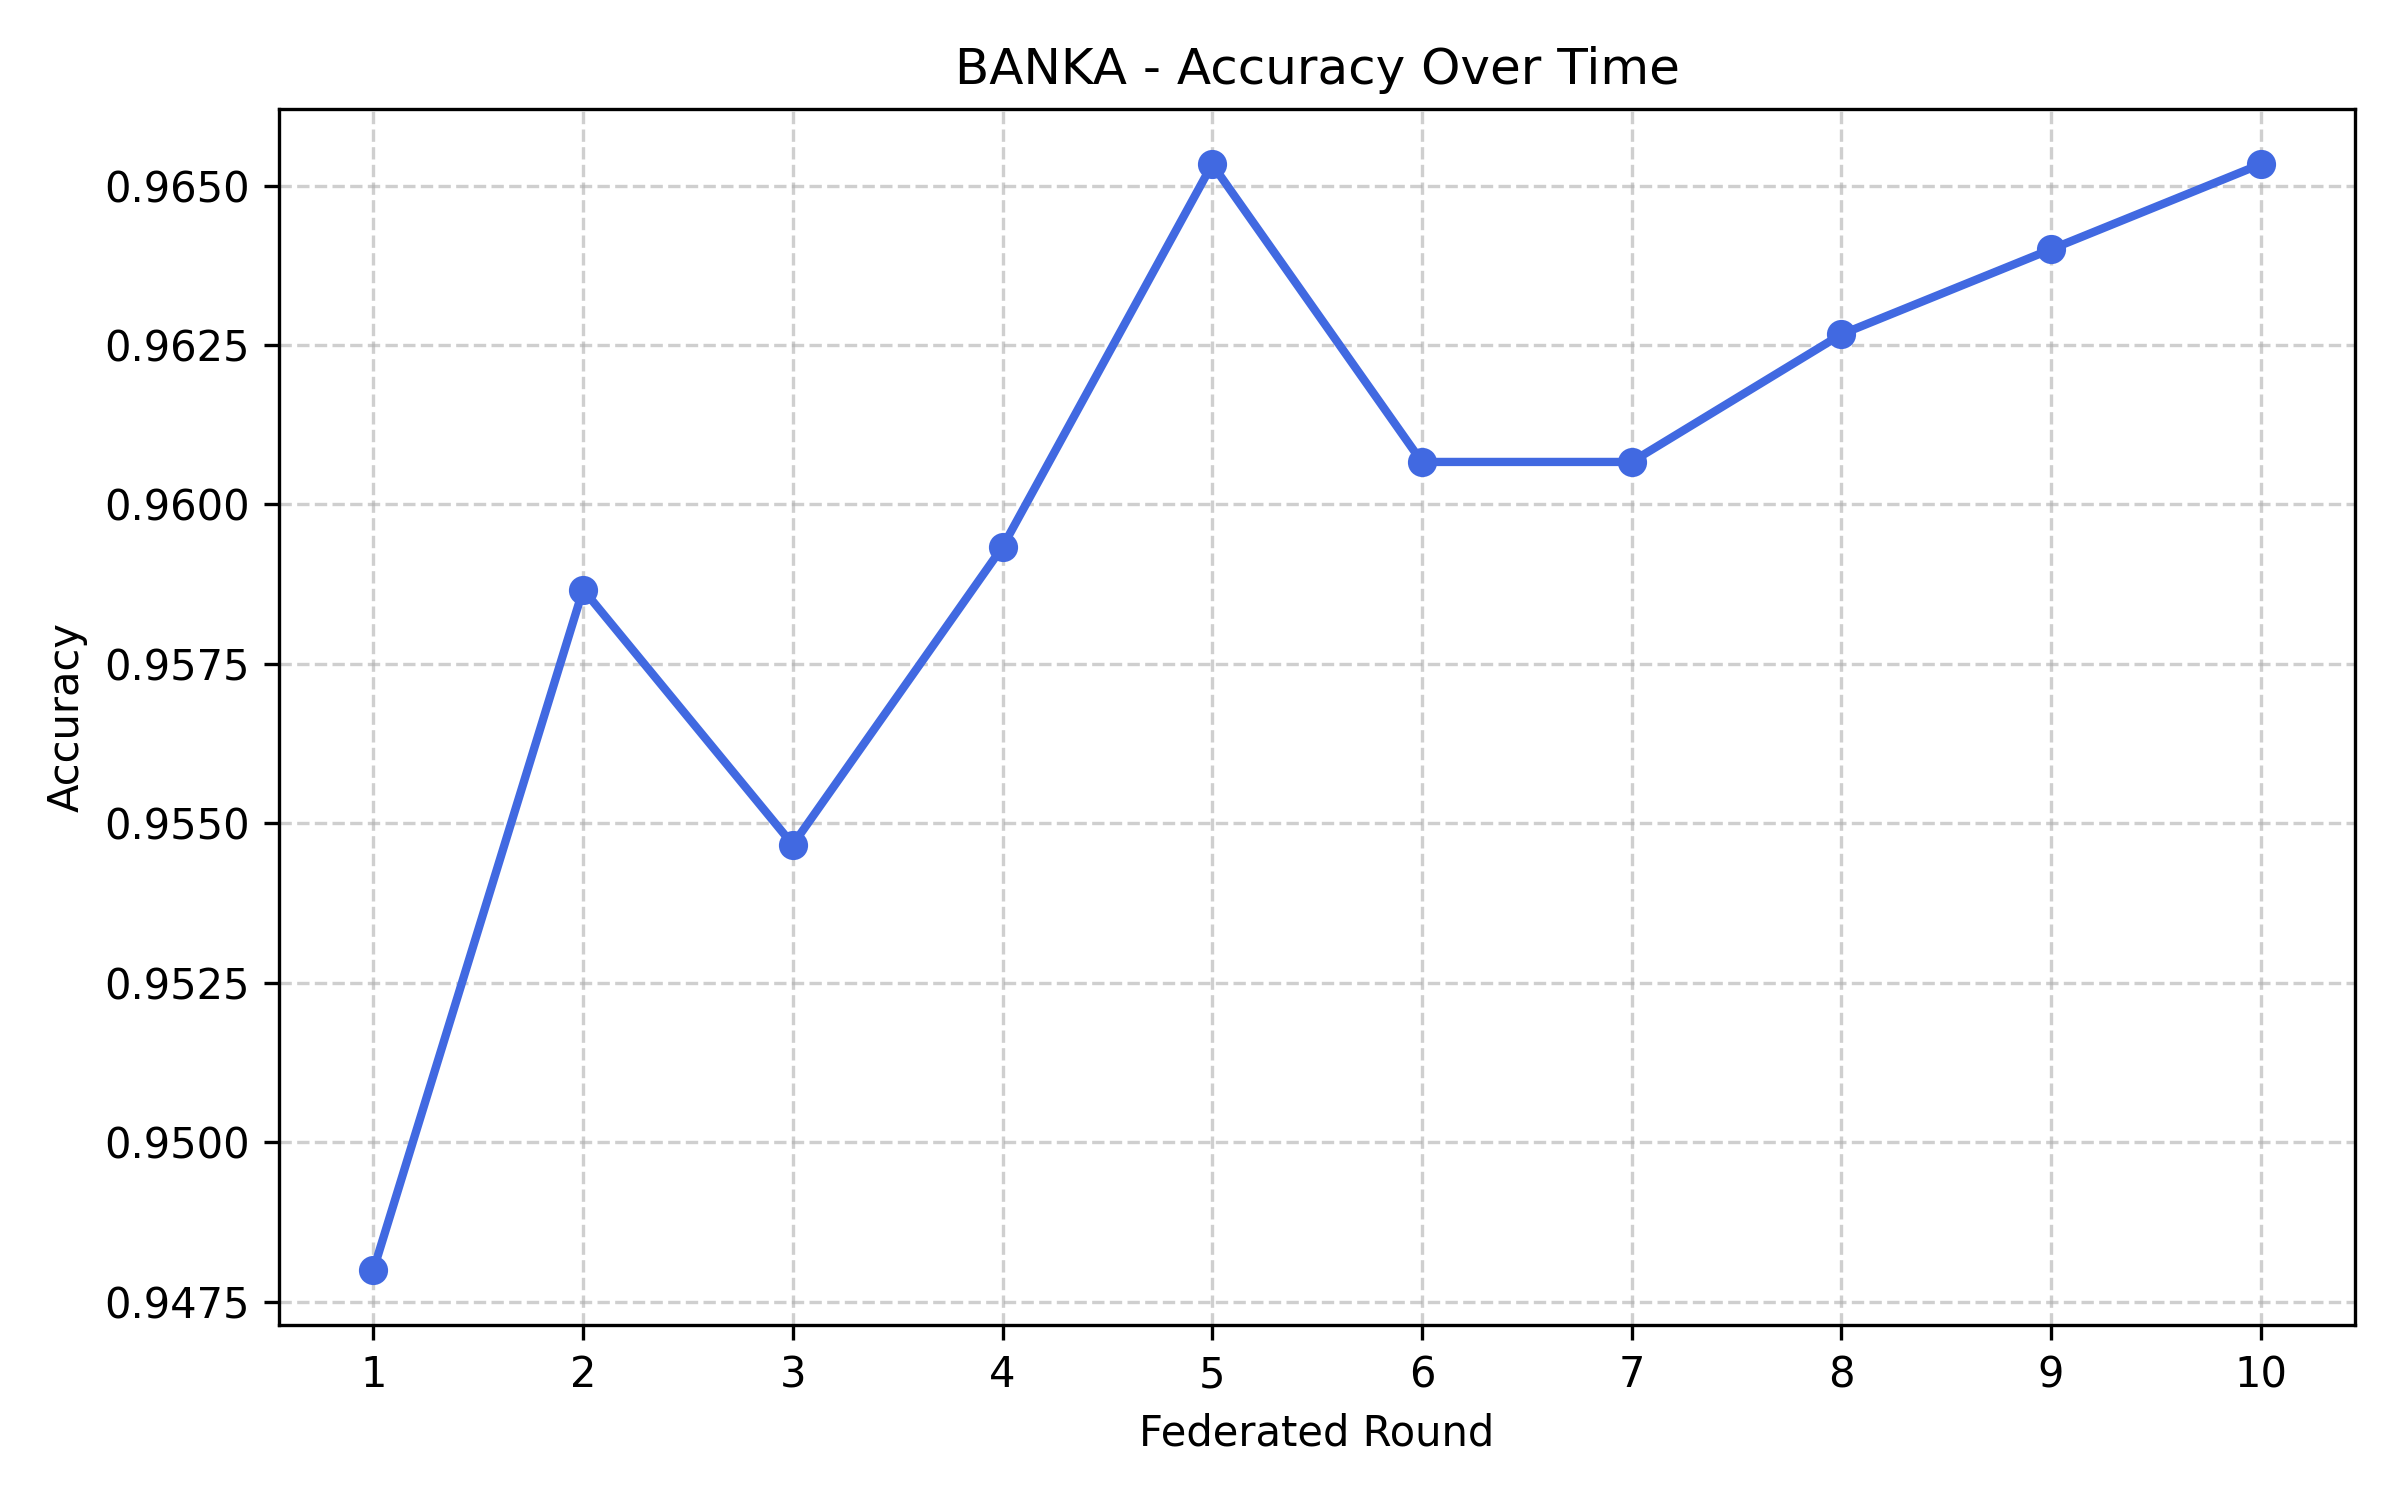
\includegraphics[width=\linewidth]{Figures/banka_progression_accuracy.png}
\end{minipage}
\hfill
\begin{minipage}{0.32\textwidth}
\centering
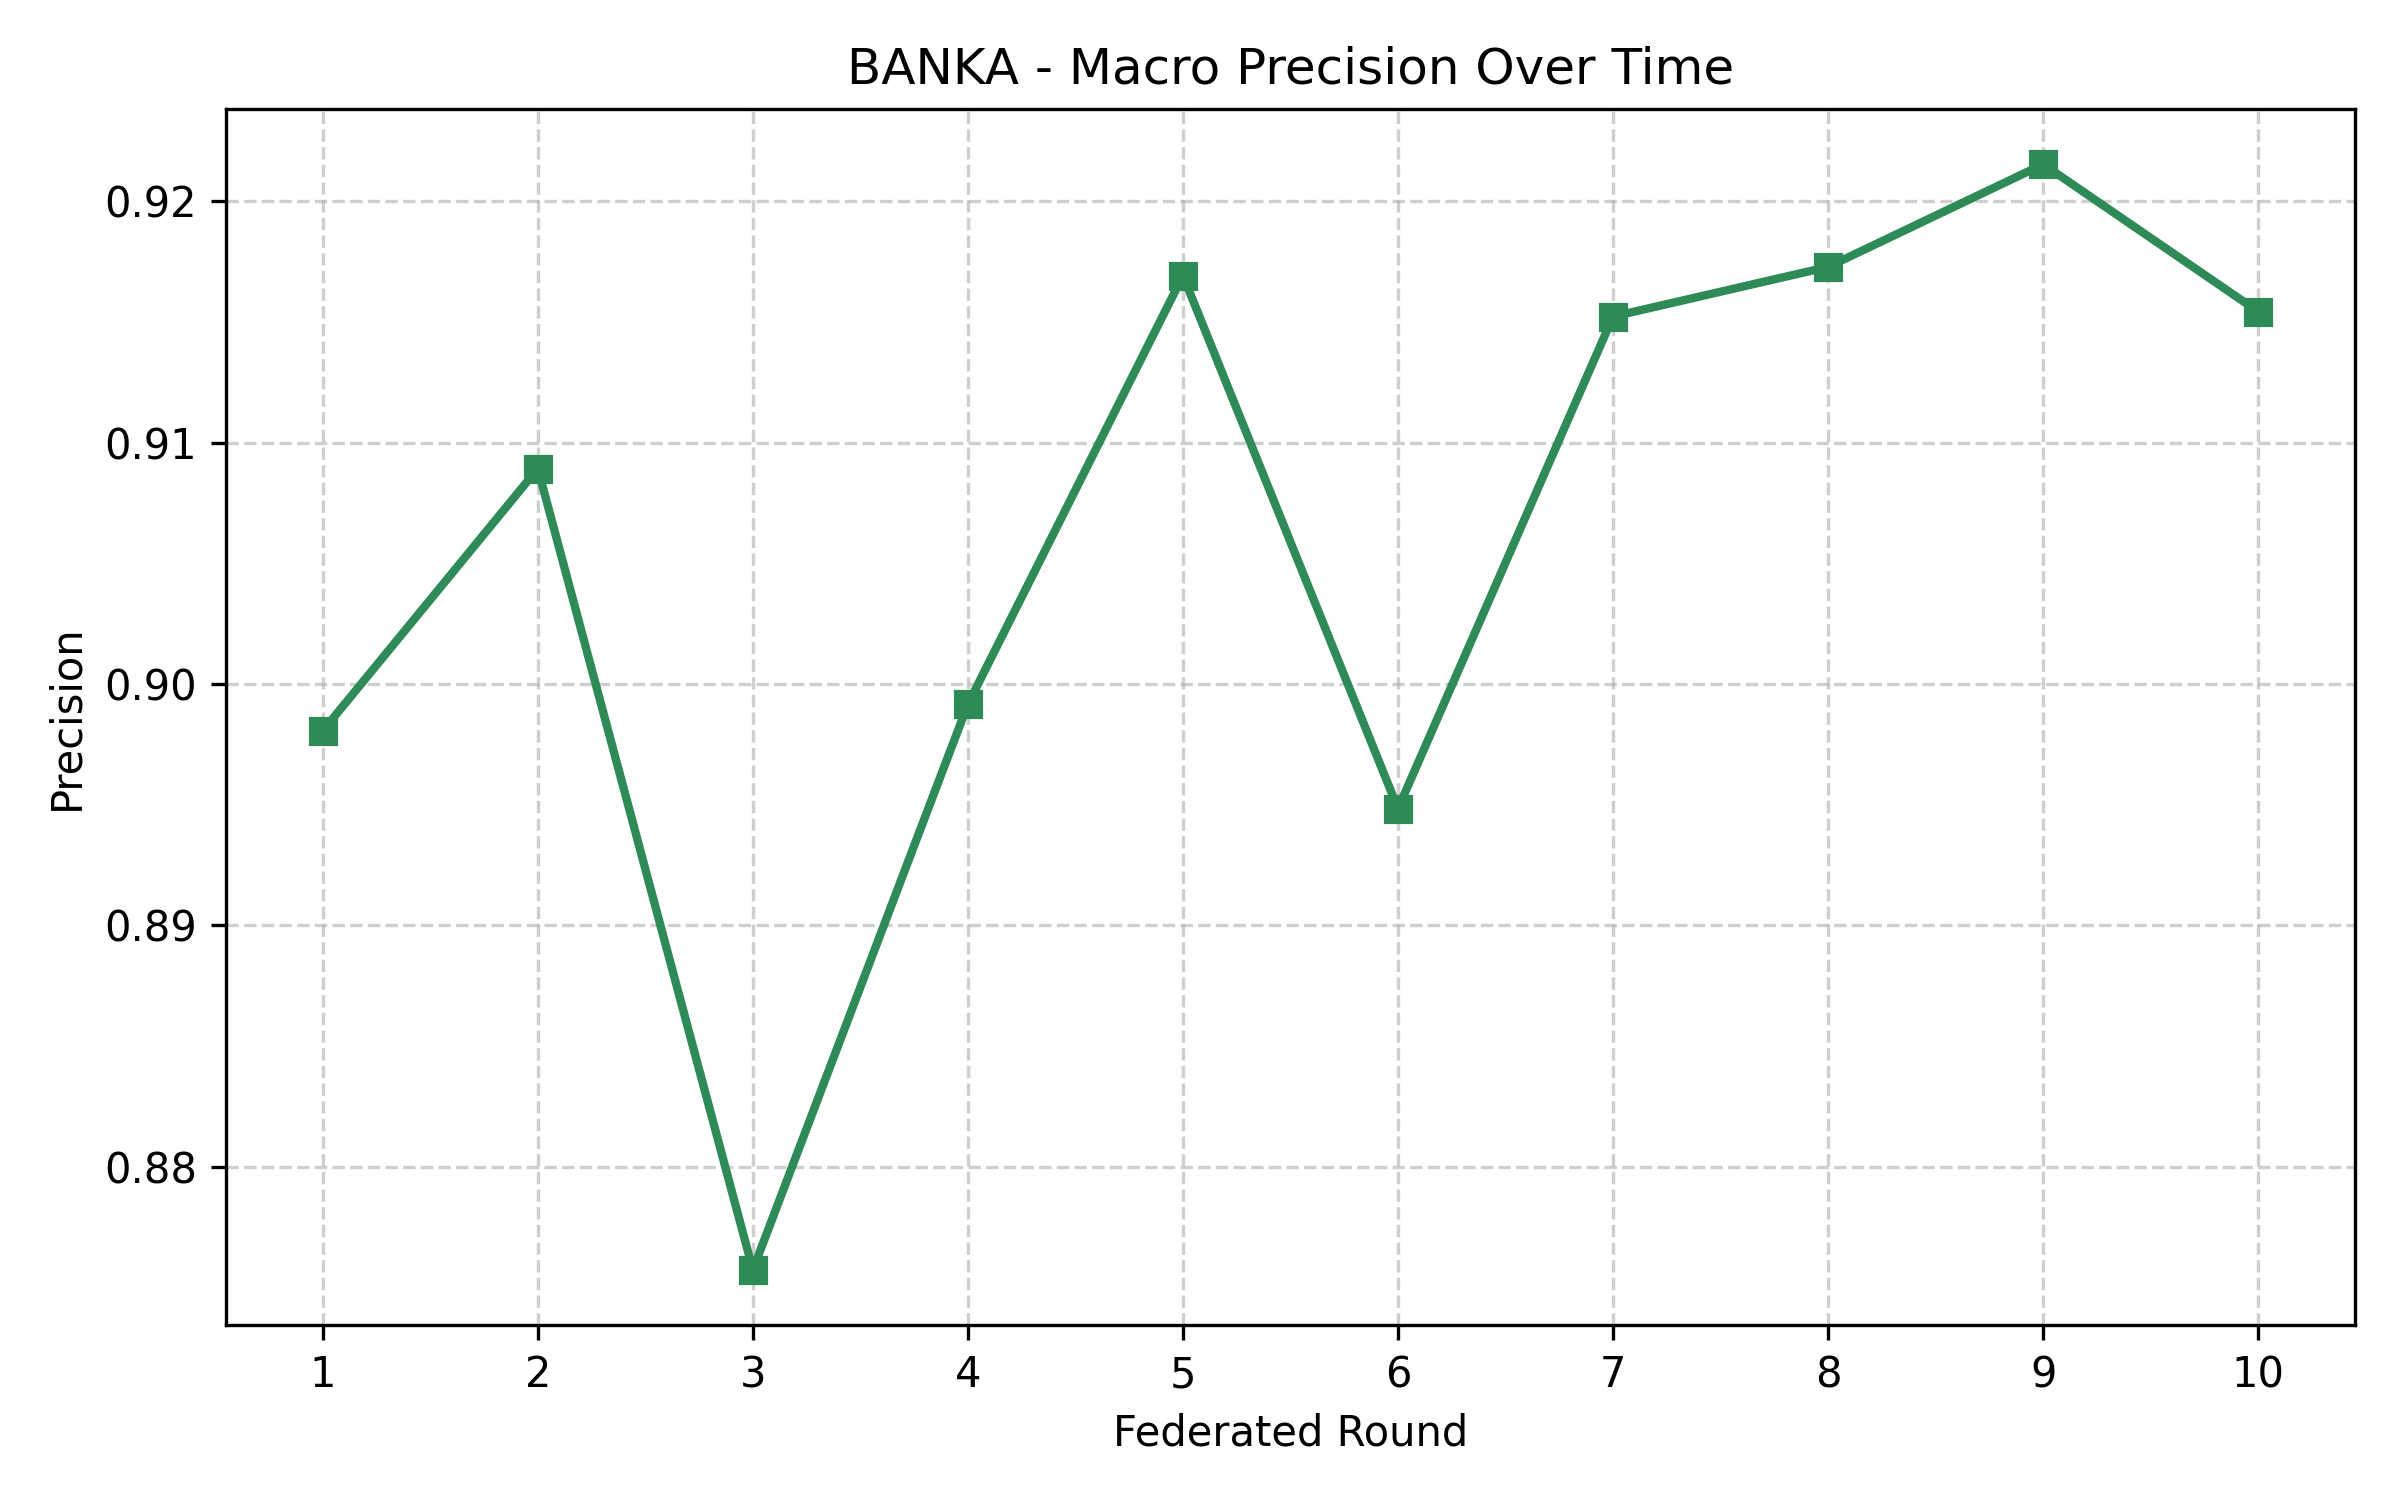
\includegraphics[width=\linewidth]{Figures/banka_progression_precision.png}
\end{minipage}
\hfill
\begin{minipage}{0.32\textwidth}
\centering
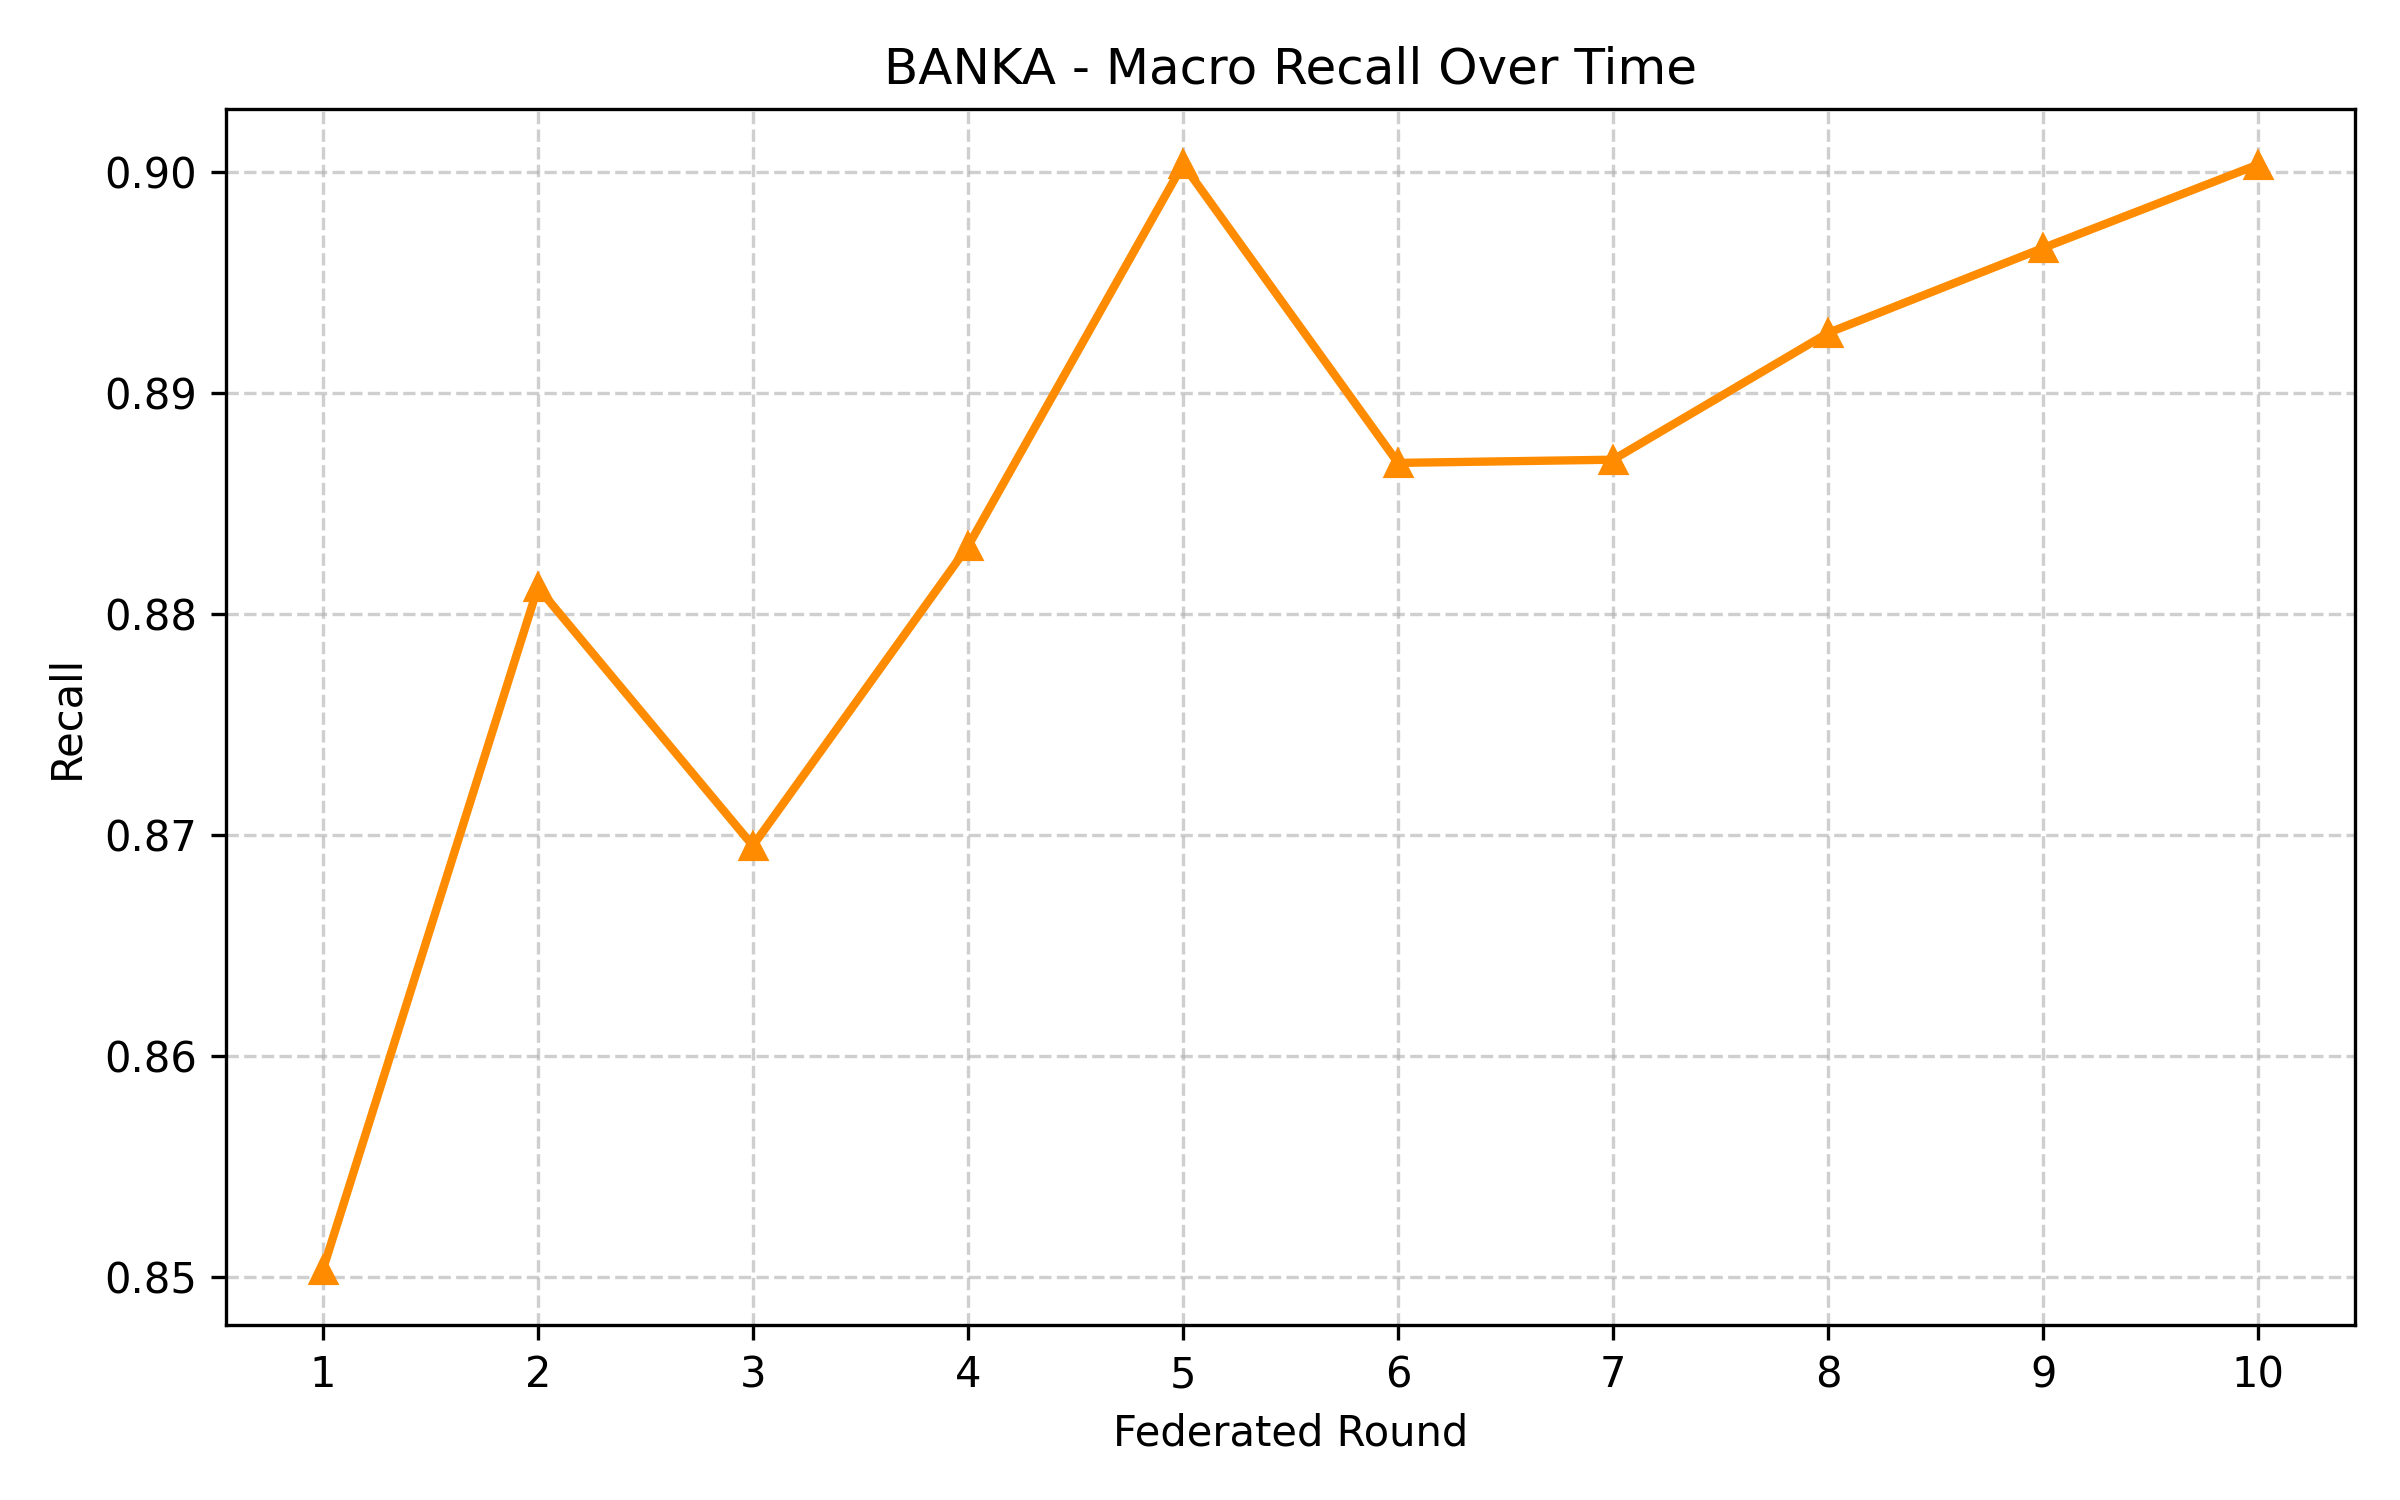
\includegraphics[width=\linewidth]{Figures/banka_progression_recall.png}
\end{minipage}

\caption{BANKA Federated Accuracy, Precision, and Recall Progression Across Federated Aggregation Rounds}
\label{fig:banka_progression}
\end{figure}

As shown in Figure~\ref{fig:banka_progression}, BANKA showed the expected training dynamics for a federated setup. The early variation was reduced as global aggregation and distributed weight synchronization started to dominate the optimization process, and the Accuracy, Precision, and Recall curves became noticeably smoother in the later rounds. That pattern indicates that the client was converging in a controlled way and that the federated updates were being integrated properly.
%--------------------------------------------------------
\subsubsection{BANKB Federated Convergence}
%--------------------------------------------------------

\begin{figure}[H]
\centering

\begin{minipage}{0.32\textwidth}
\centering
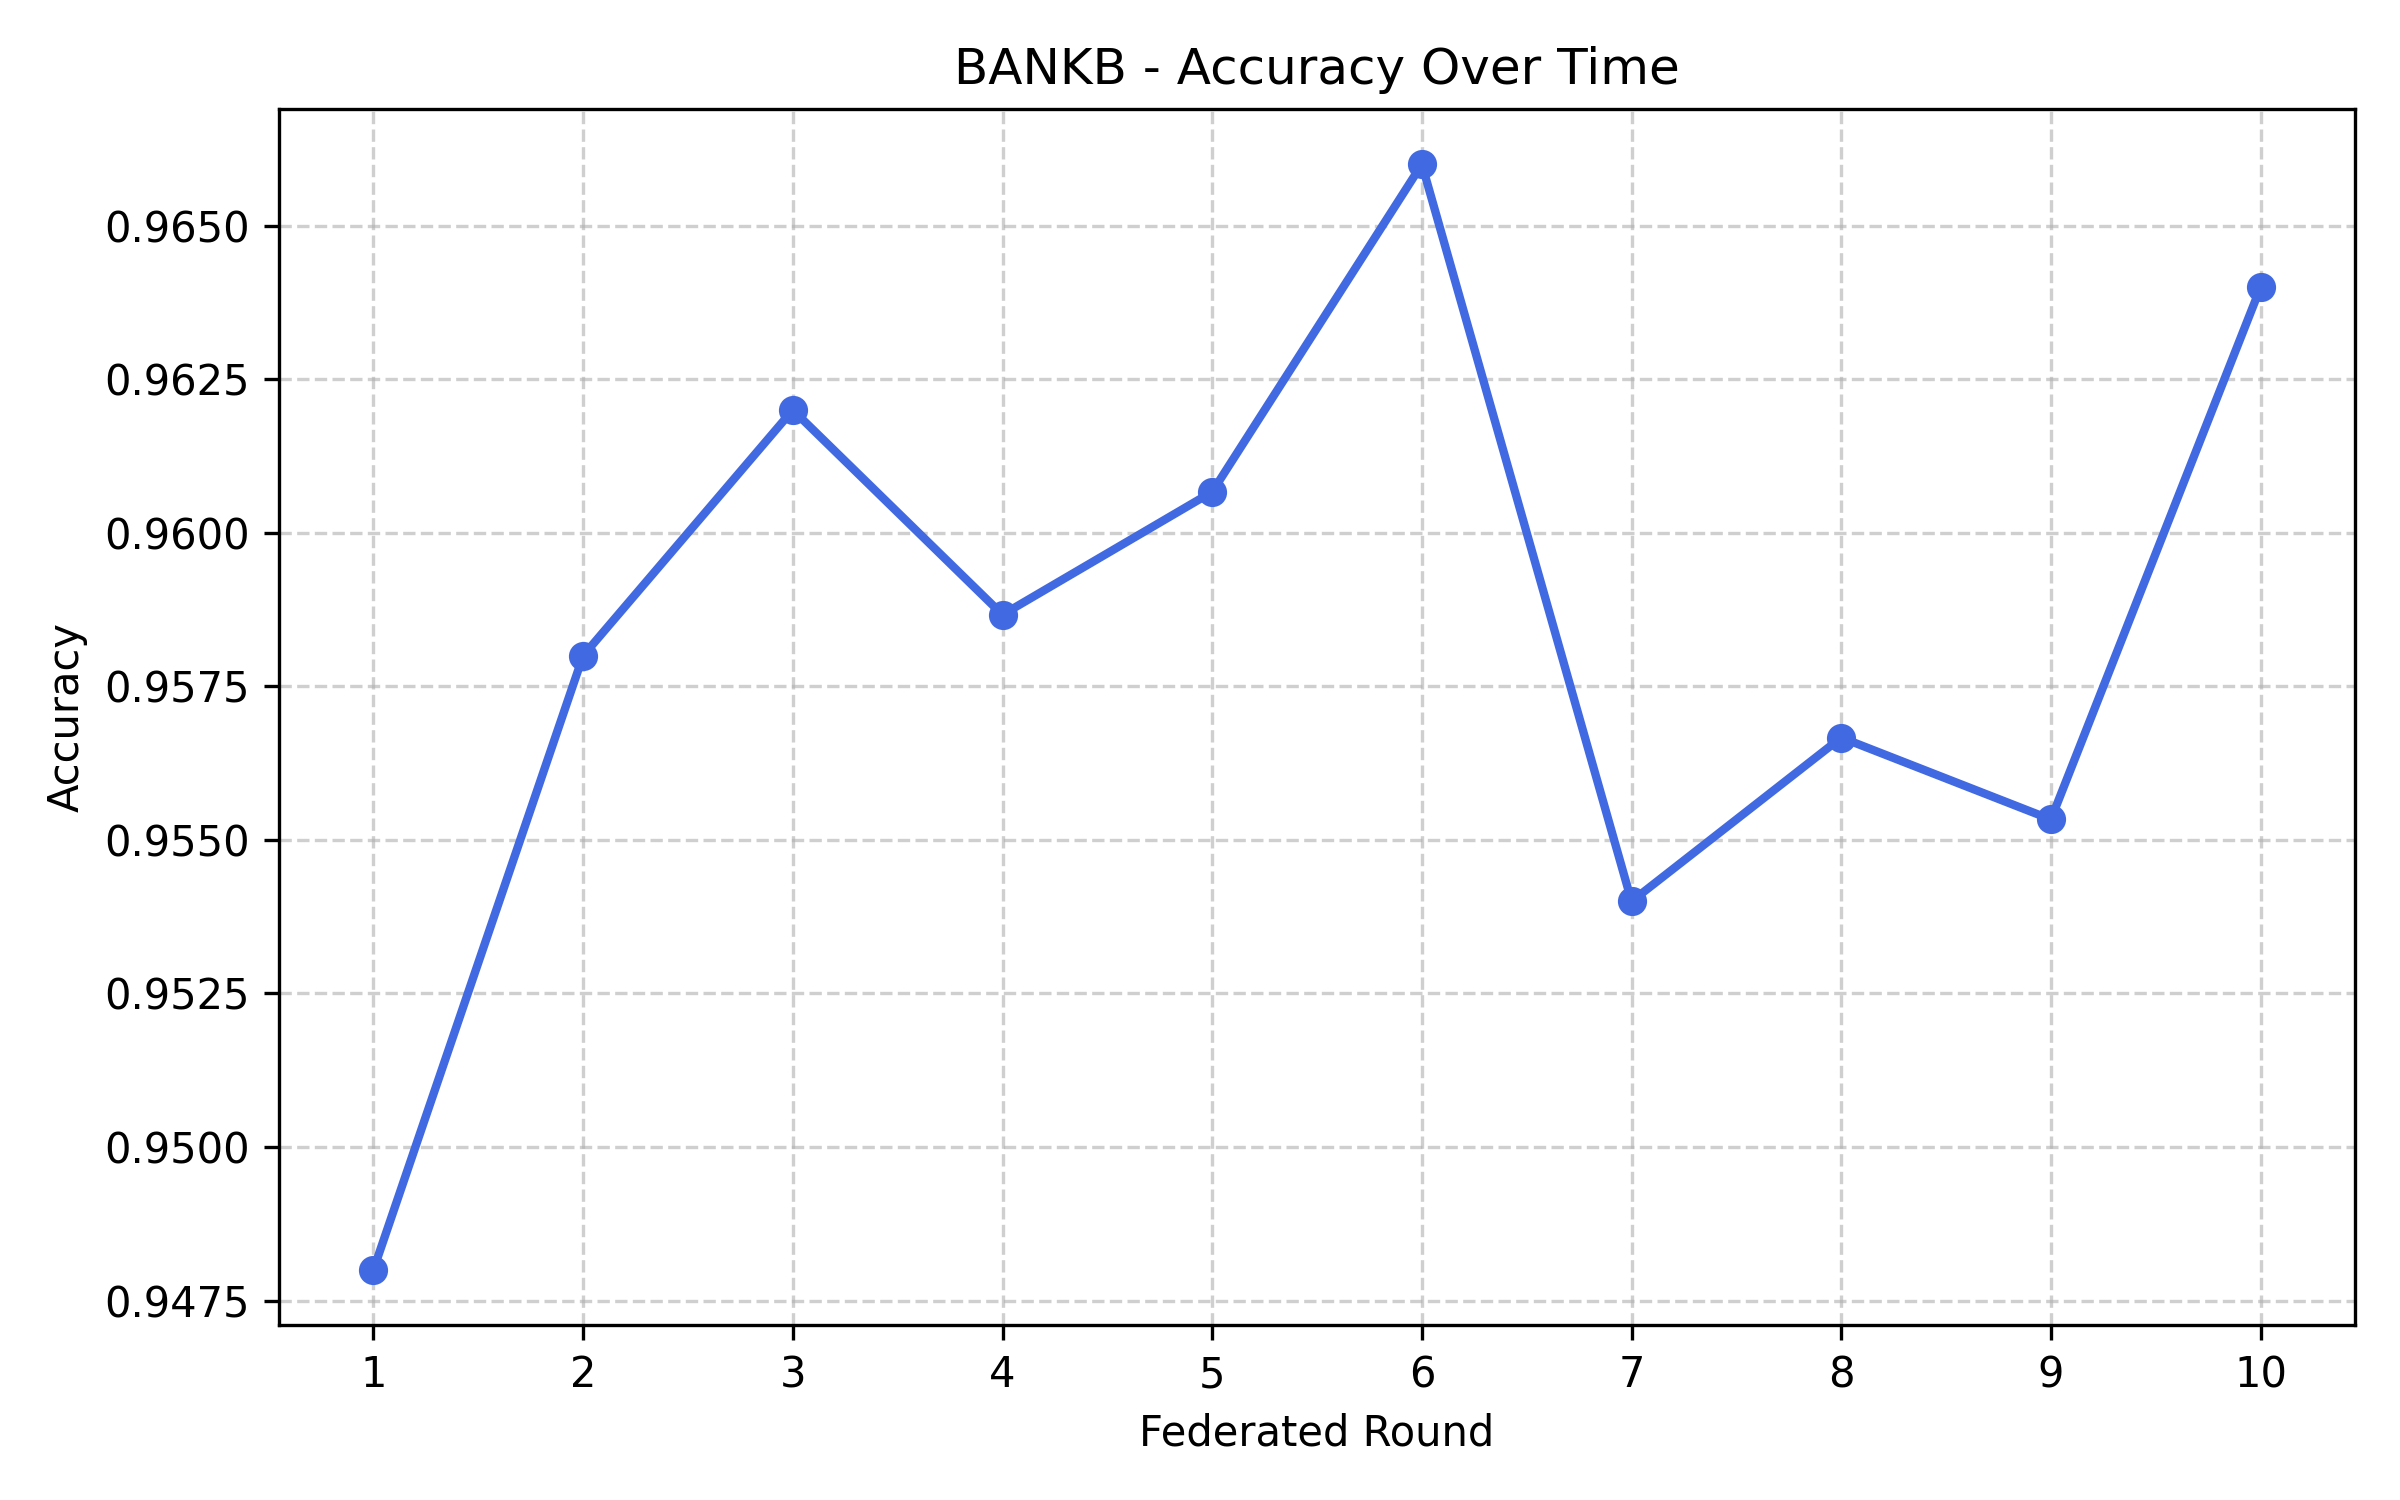
\includegraphics[width=\linewidth]{Figures/bankb_progression_accuracy.png}
\end{minipage}
\hfill
\begin{minipage}{0.32\textwidth}
\centering
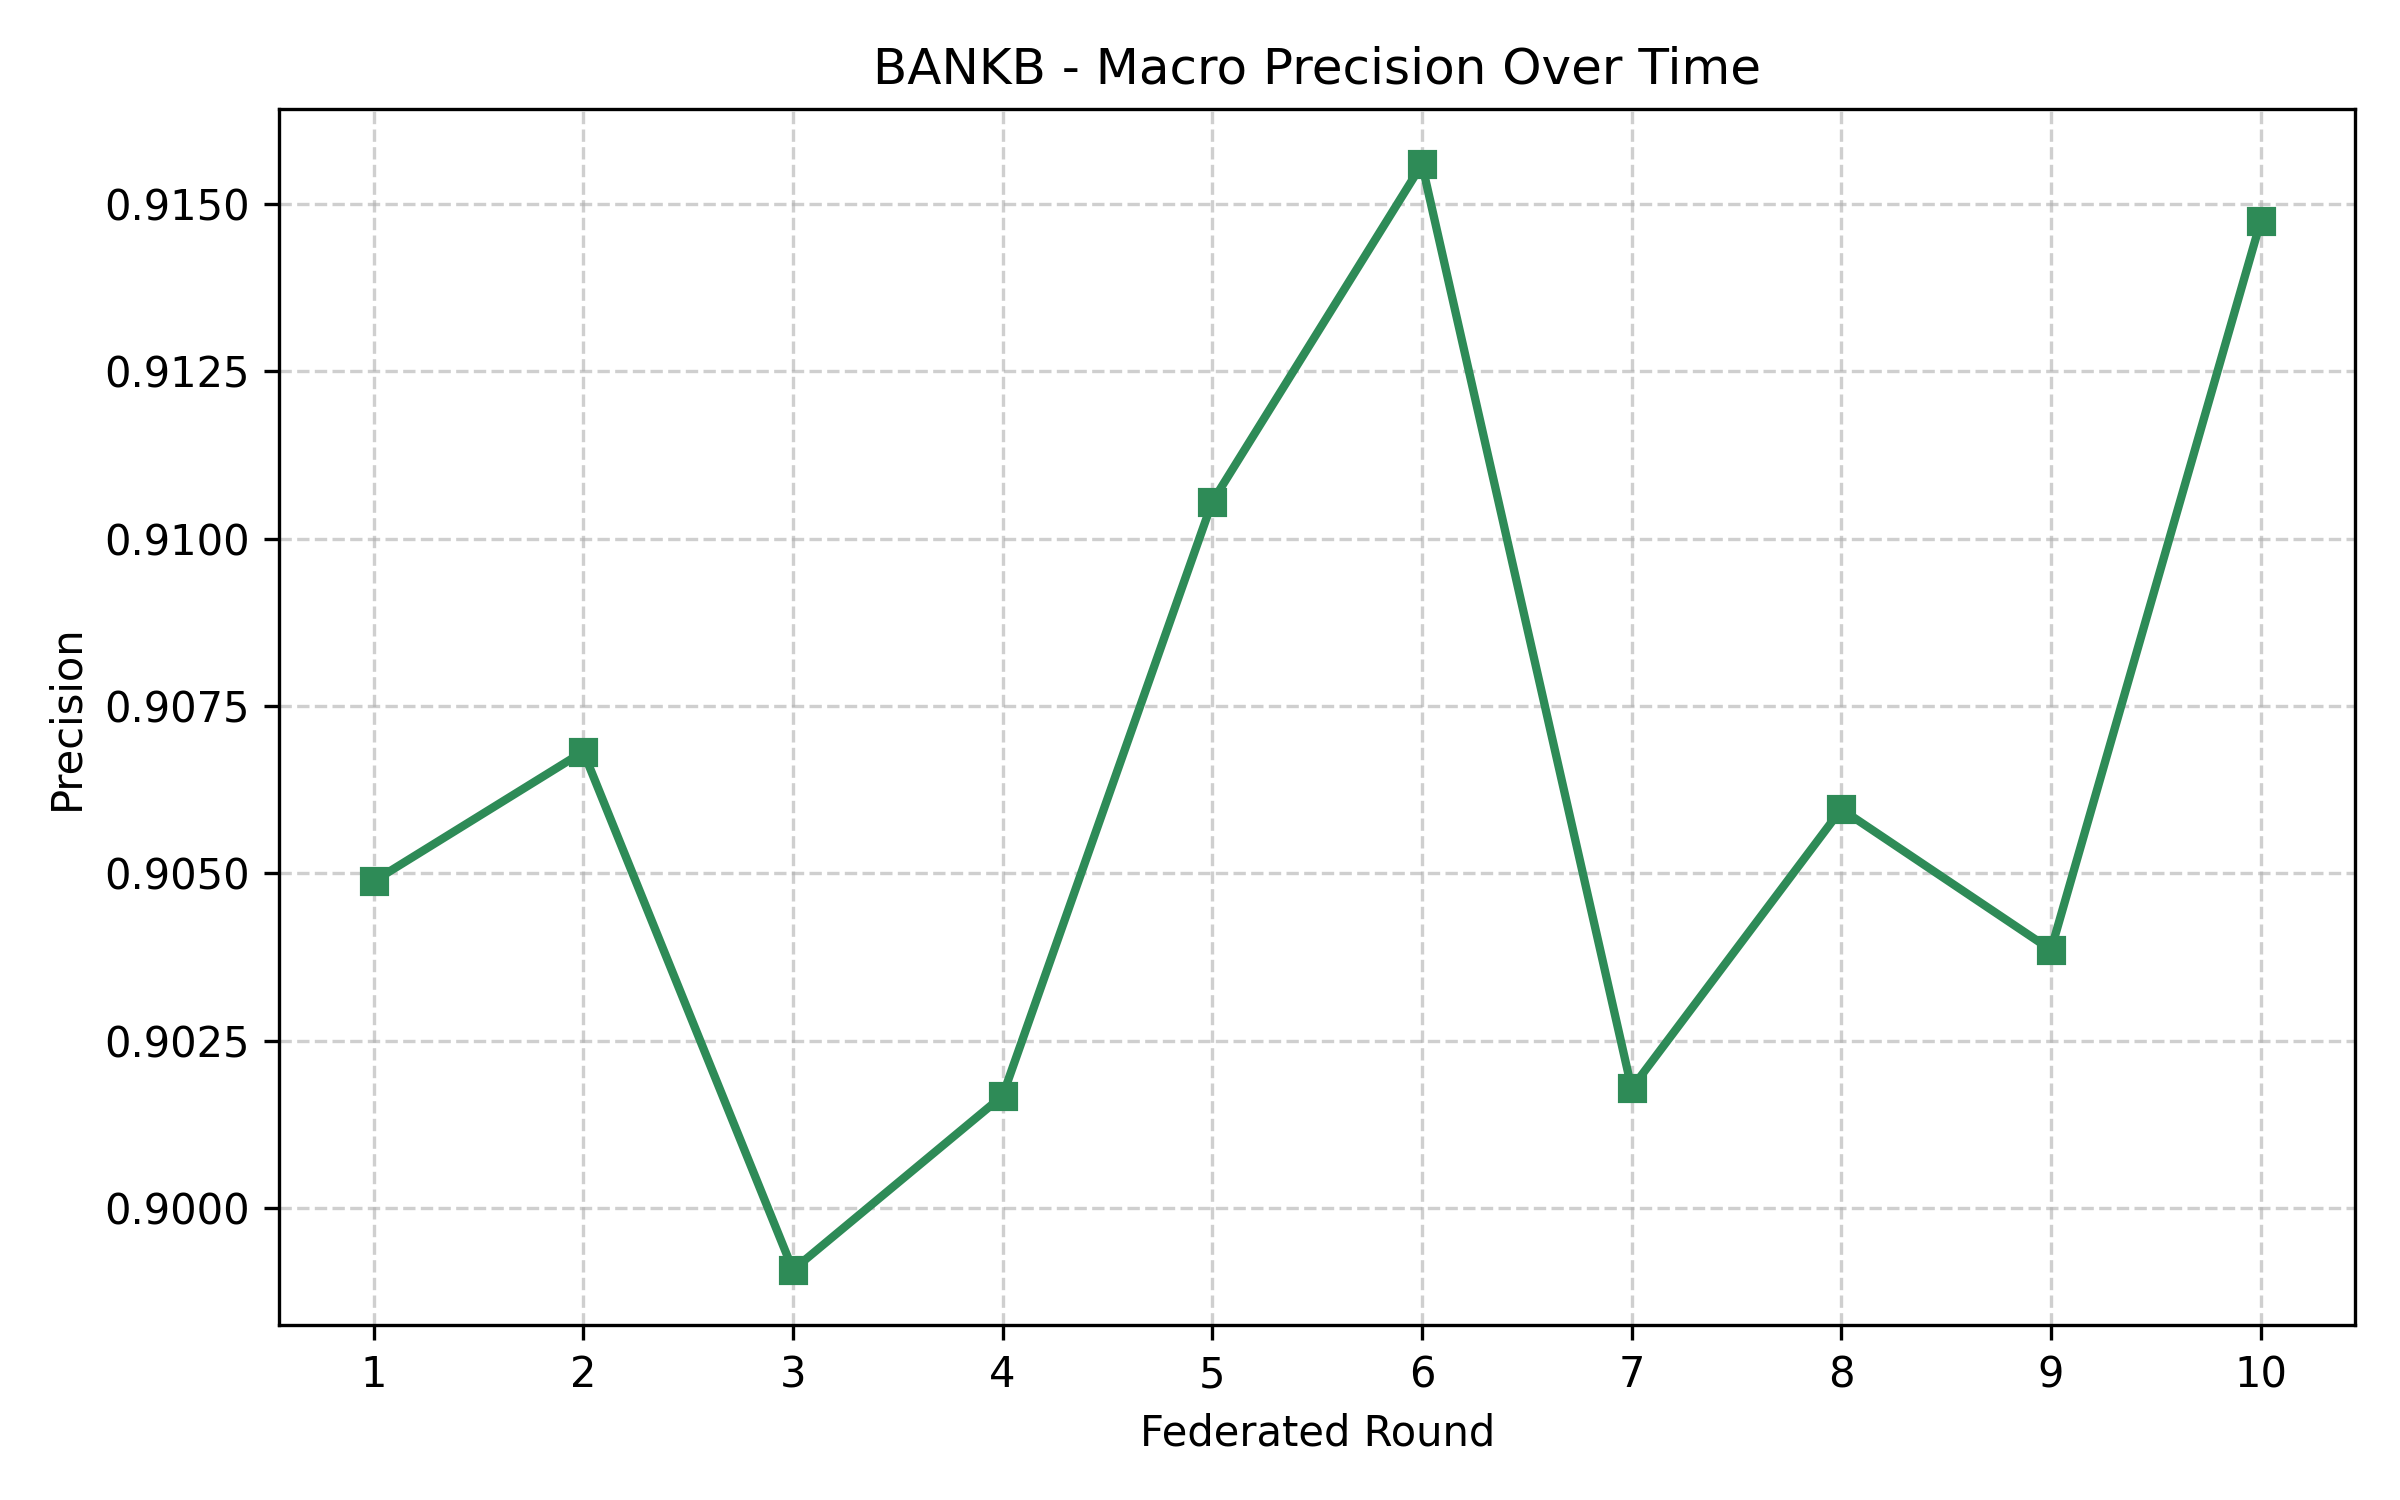
\includegraphics[width=\linewidth]{Figures/bankb_progression_precision.png}
\end{minipage}
\hfill
\begin{minipage}{0.32\textwidth}
\centering
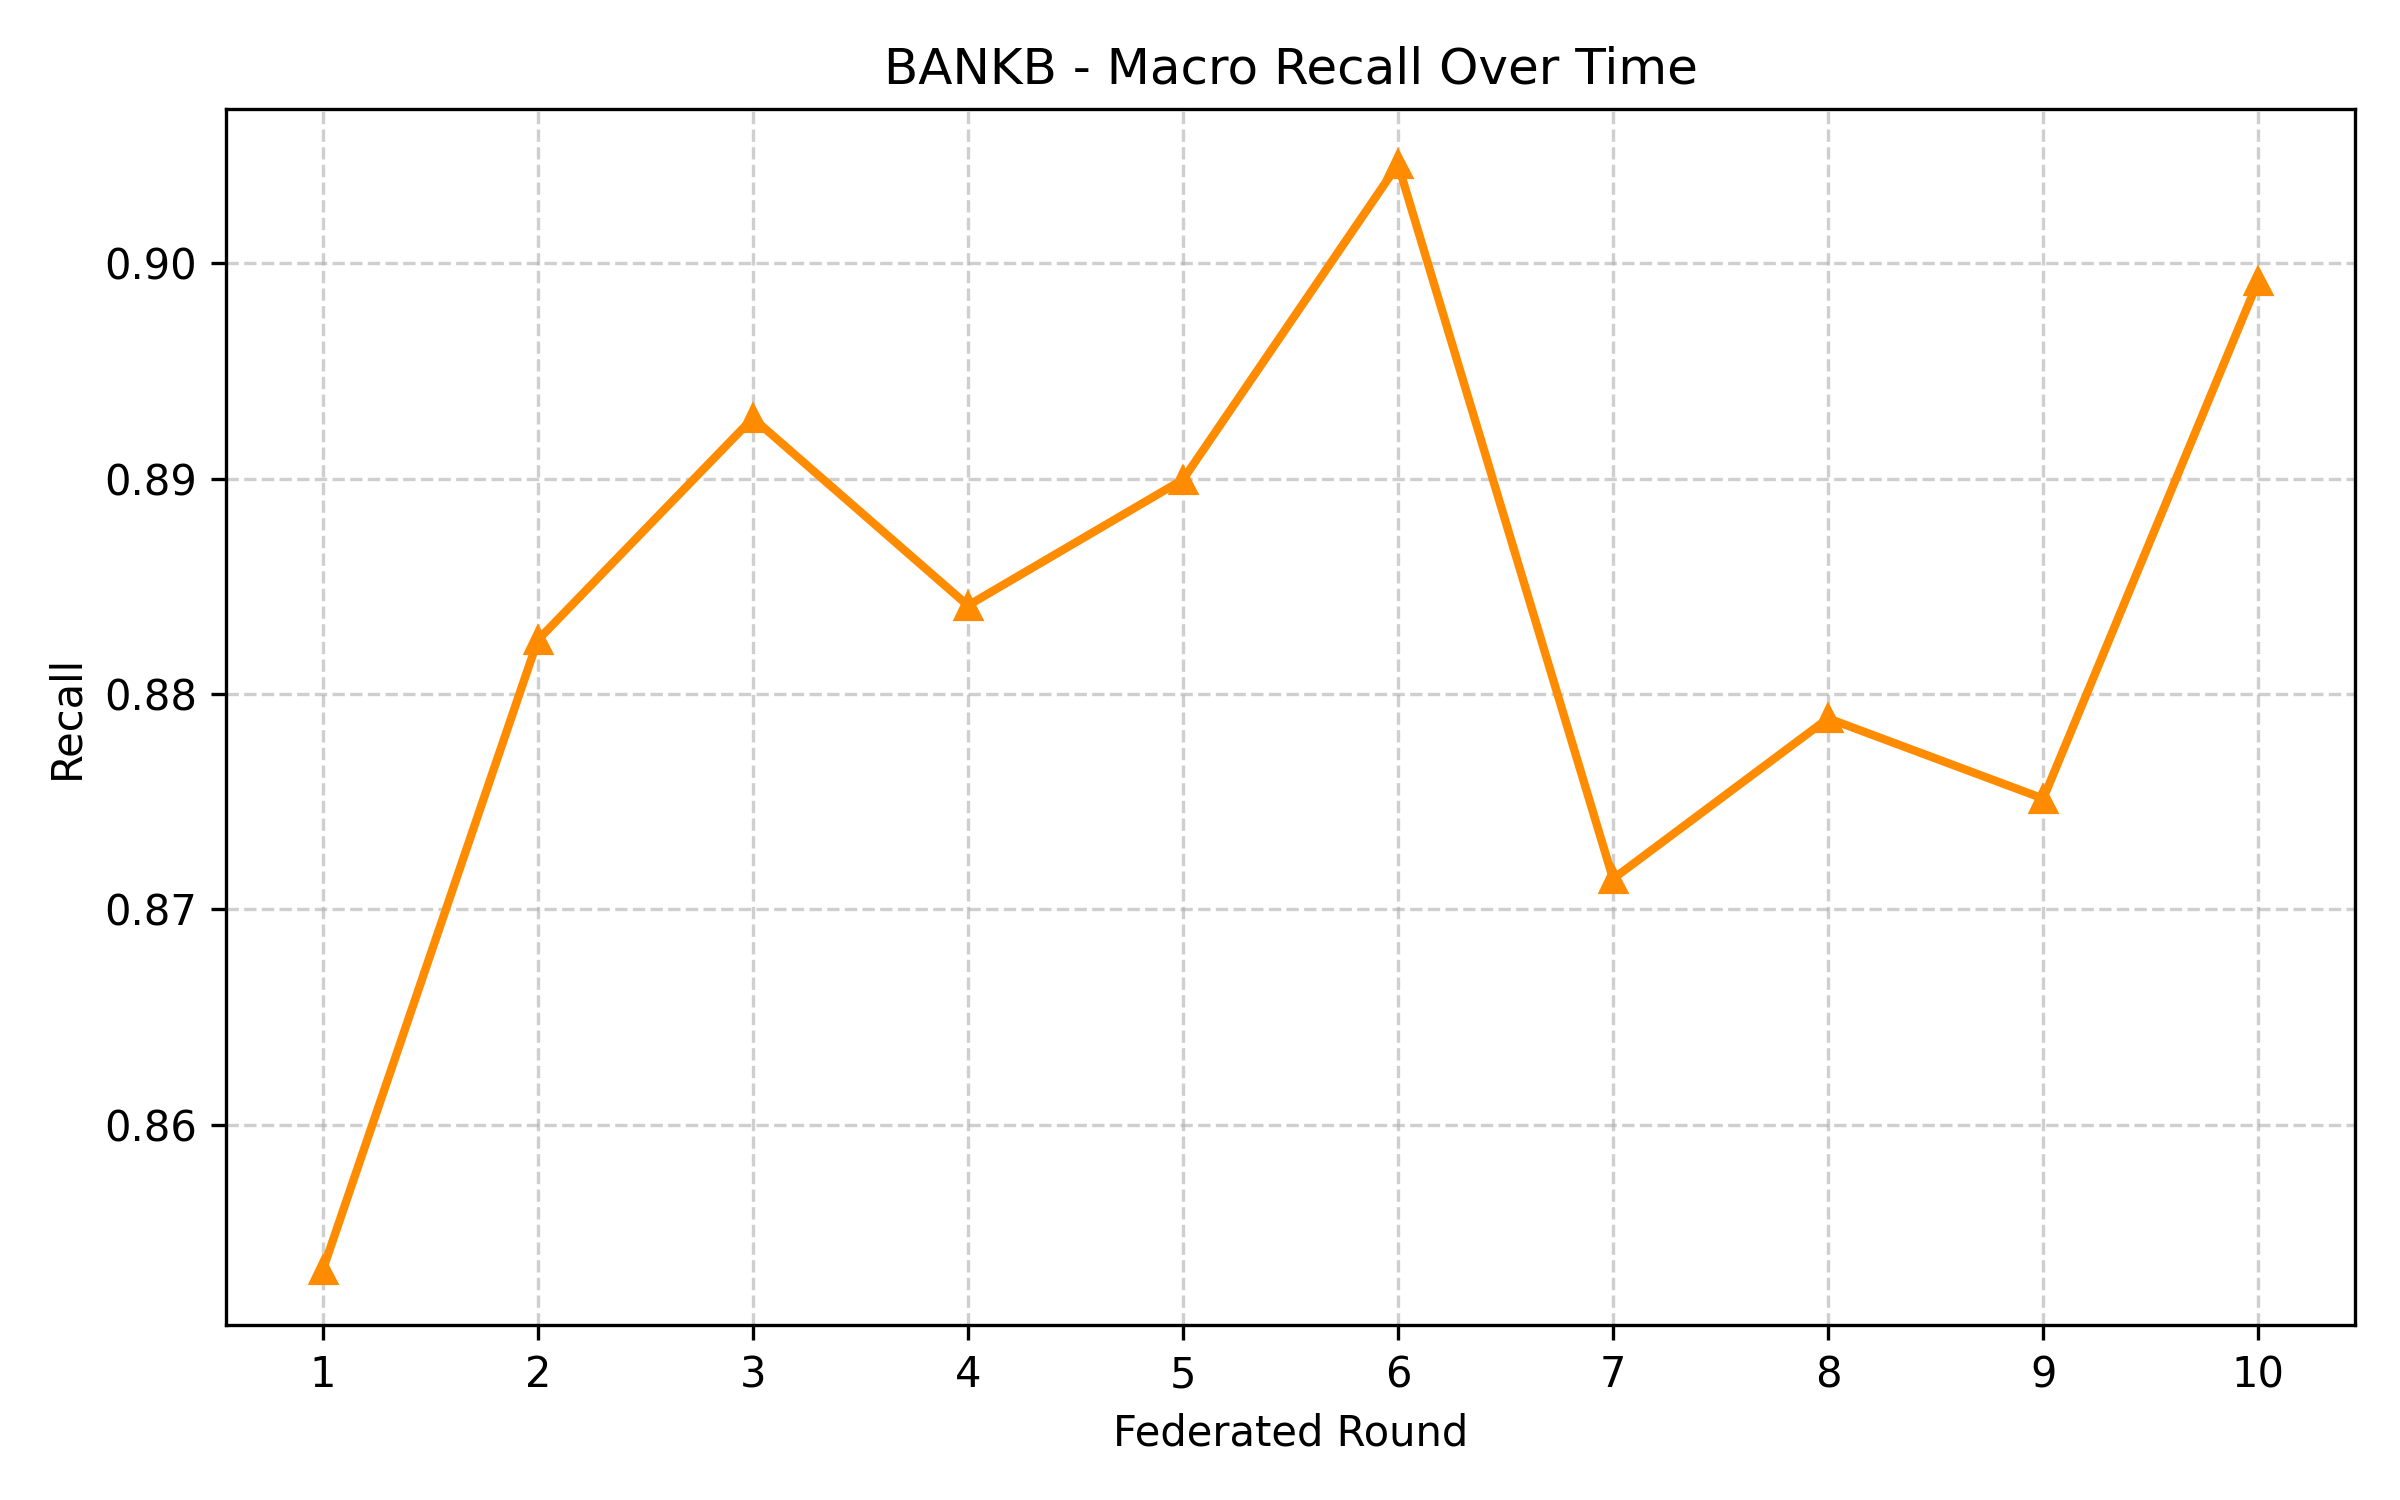
\includegraphics[width=\linewidth]{Figures/bankb_progression_recall.png}
\end{minipage}

\caption{BANKB Federated Accuracy, Precision, and Recall Progression Across Federated Aggregation Rounds}
\label{fig:bankb_progression}
\end{figure}

As shown in Figure~\ref{fig:bankb_progression}, BANKB followed the same stable convergence pattern across the training rounds. Each communication round improved the consistency of the learned parameters and reduced variance in the predictions, which is what we expect when the global model is being updated from multiple institutional clients. The smoother progression confirms that cross-bank parameter sharing and distributed learning were operating correctly.
%--------------------------------------------------------
\subsubsection{BANKC Federated Convergence}
%--------------------------------------------------------

\begin{figure}[H]
\centering

\begin{minipage}{0.32\textwidth}
\centering
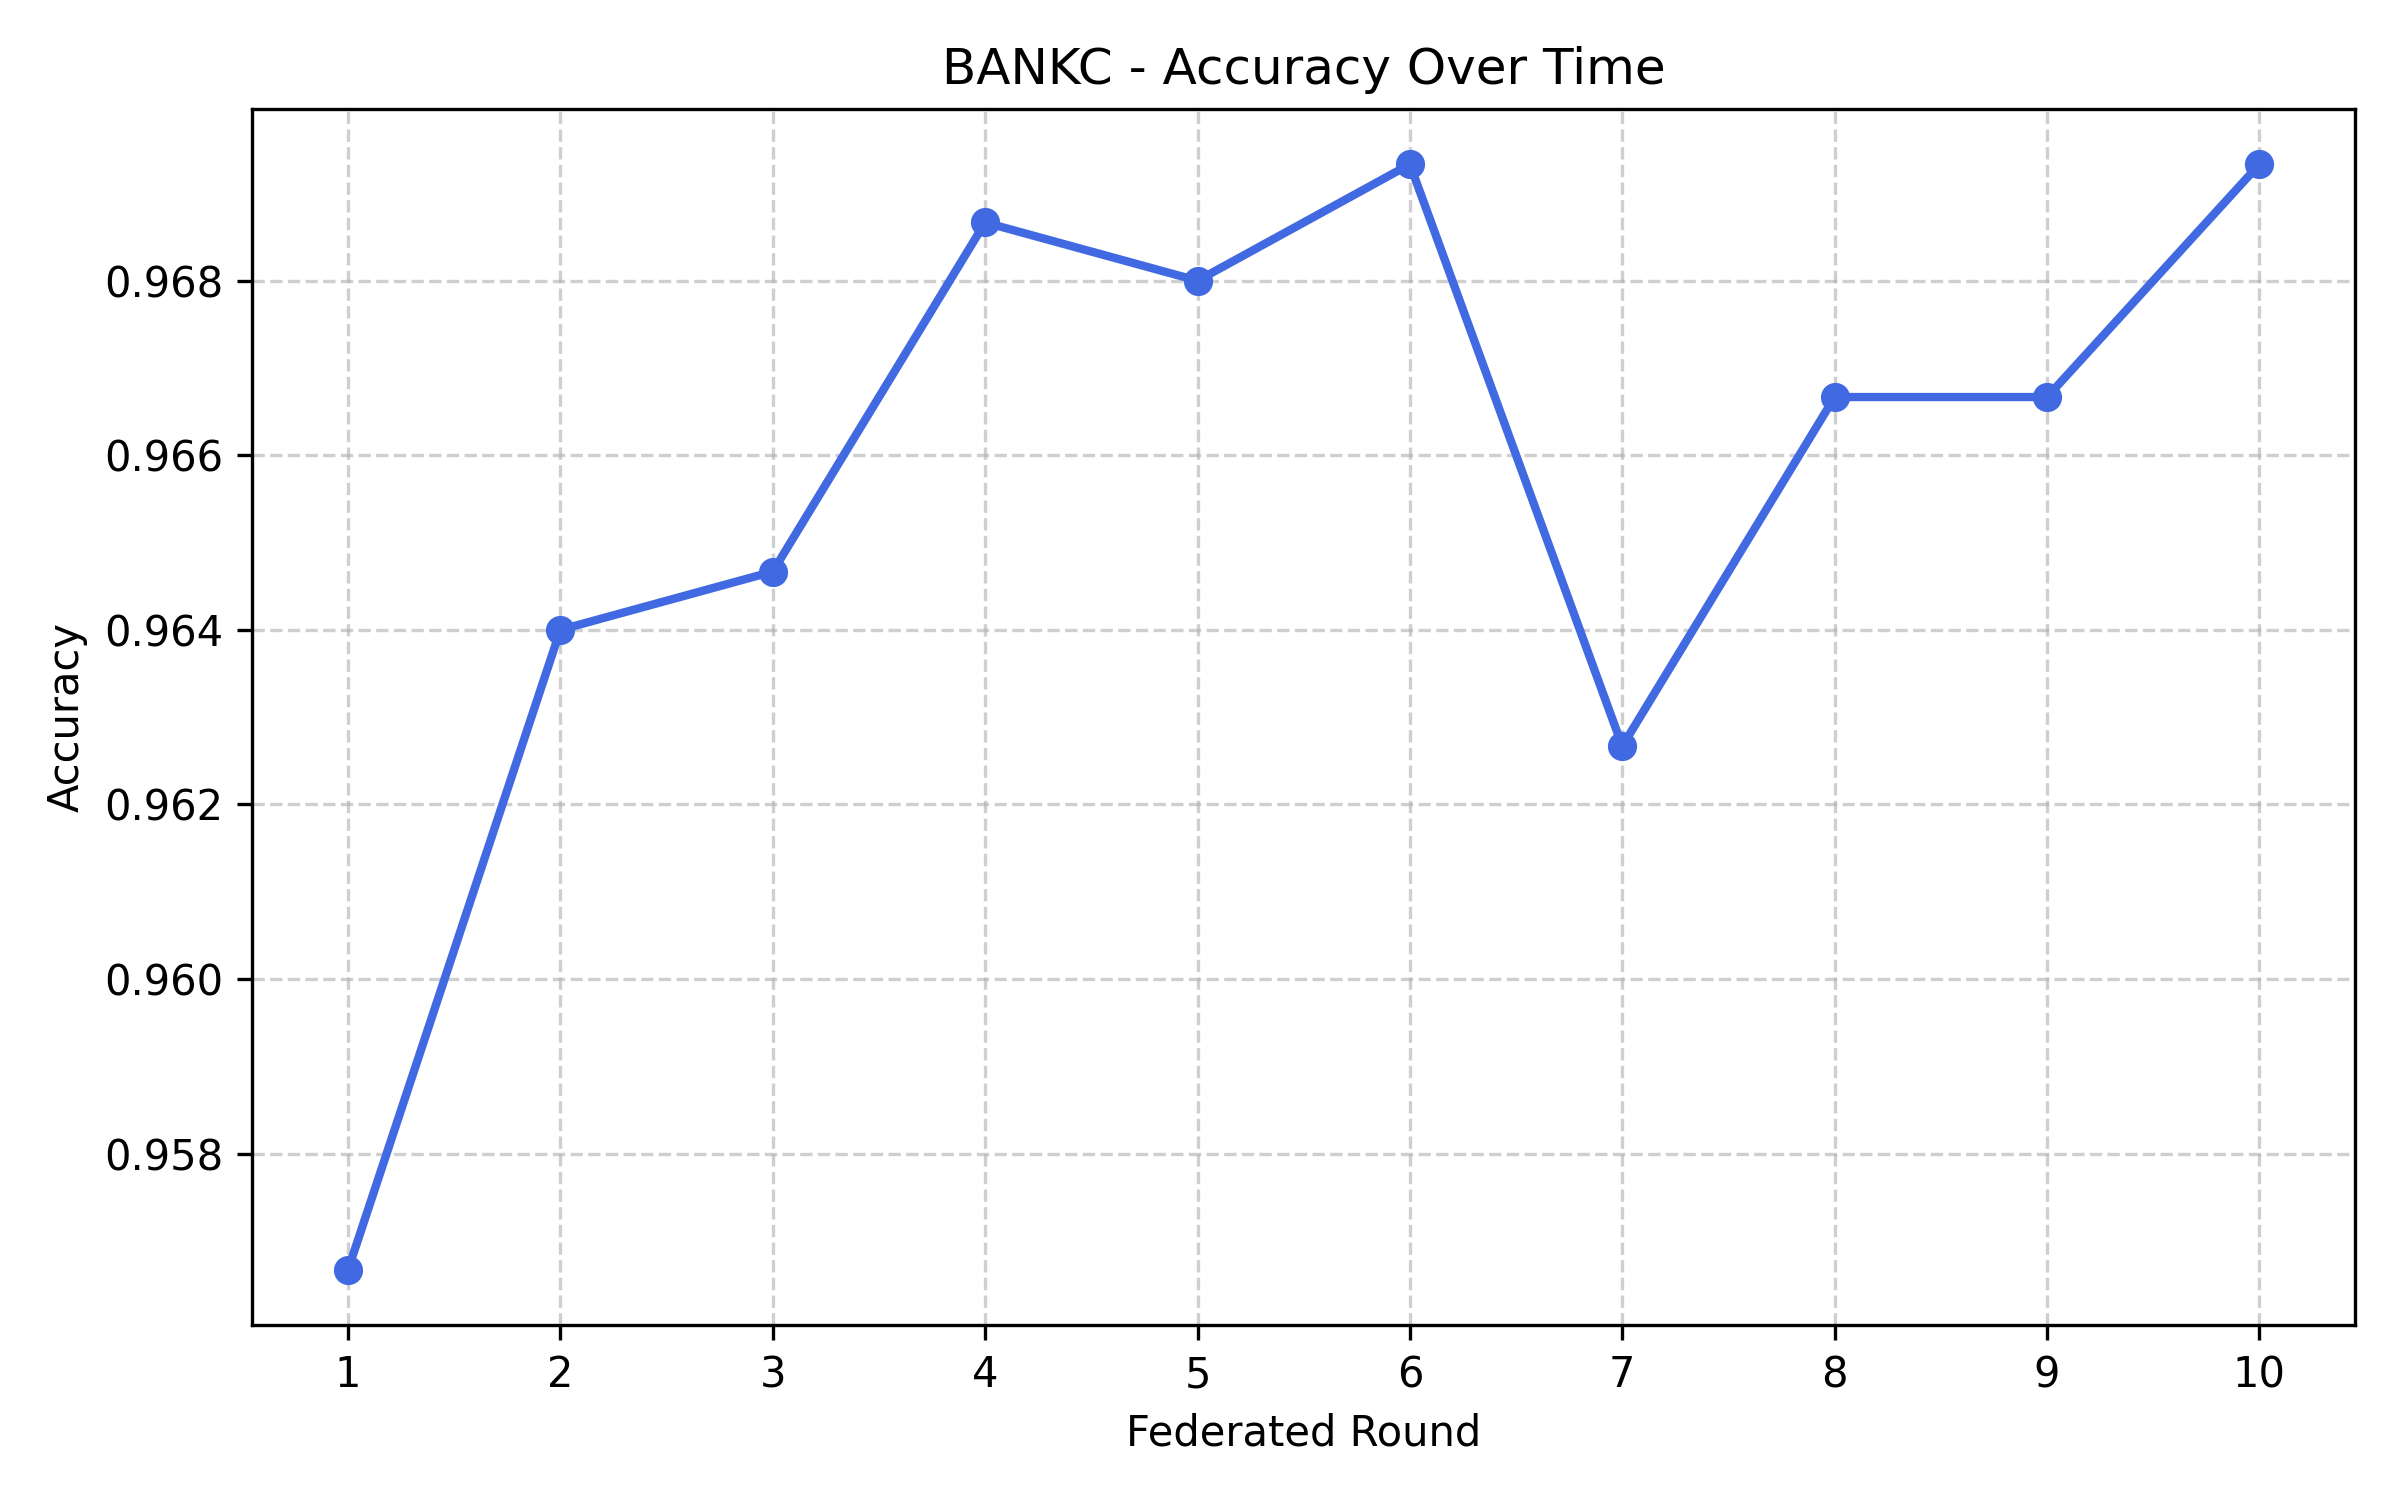
\includegraphics[width=\linewidth]{Figures/bankc_progression_accuracy.png}
\end{minipage}
\hfill
\begin{minipage}{0.32\textwidth}
\centering
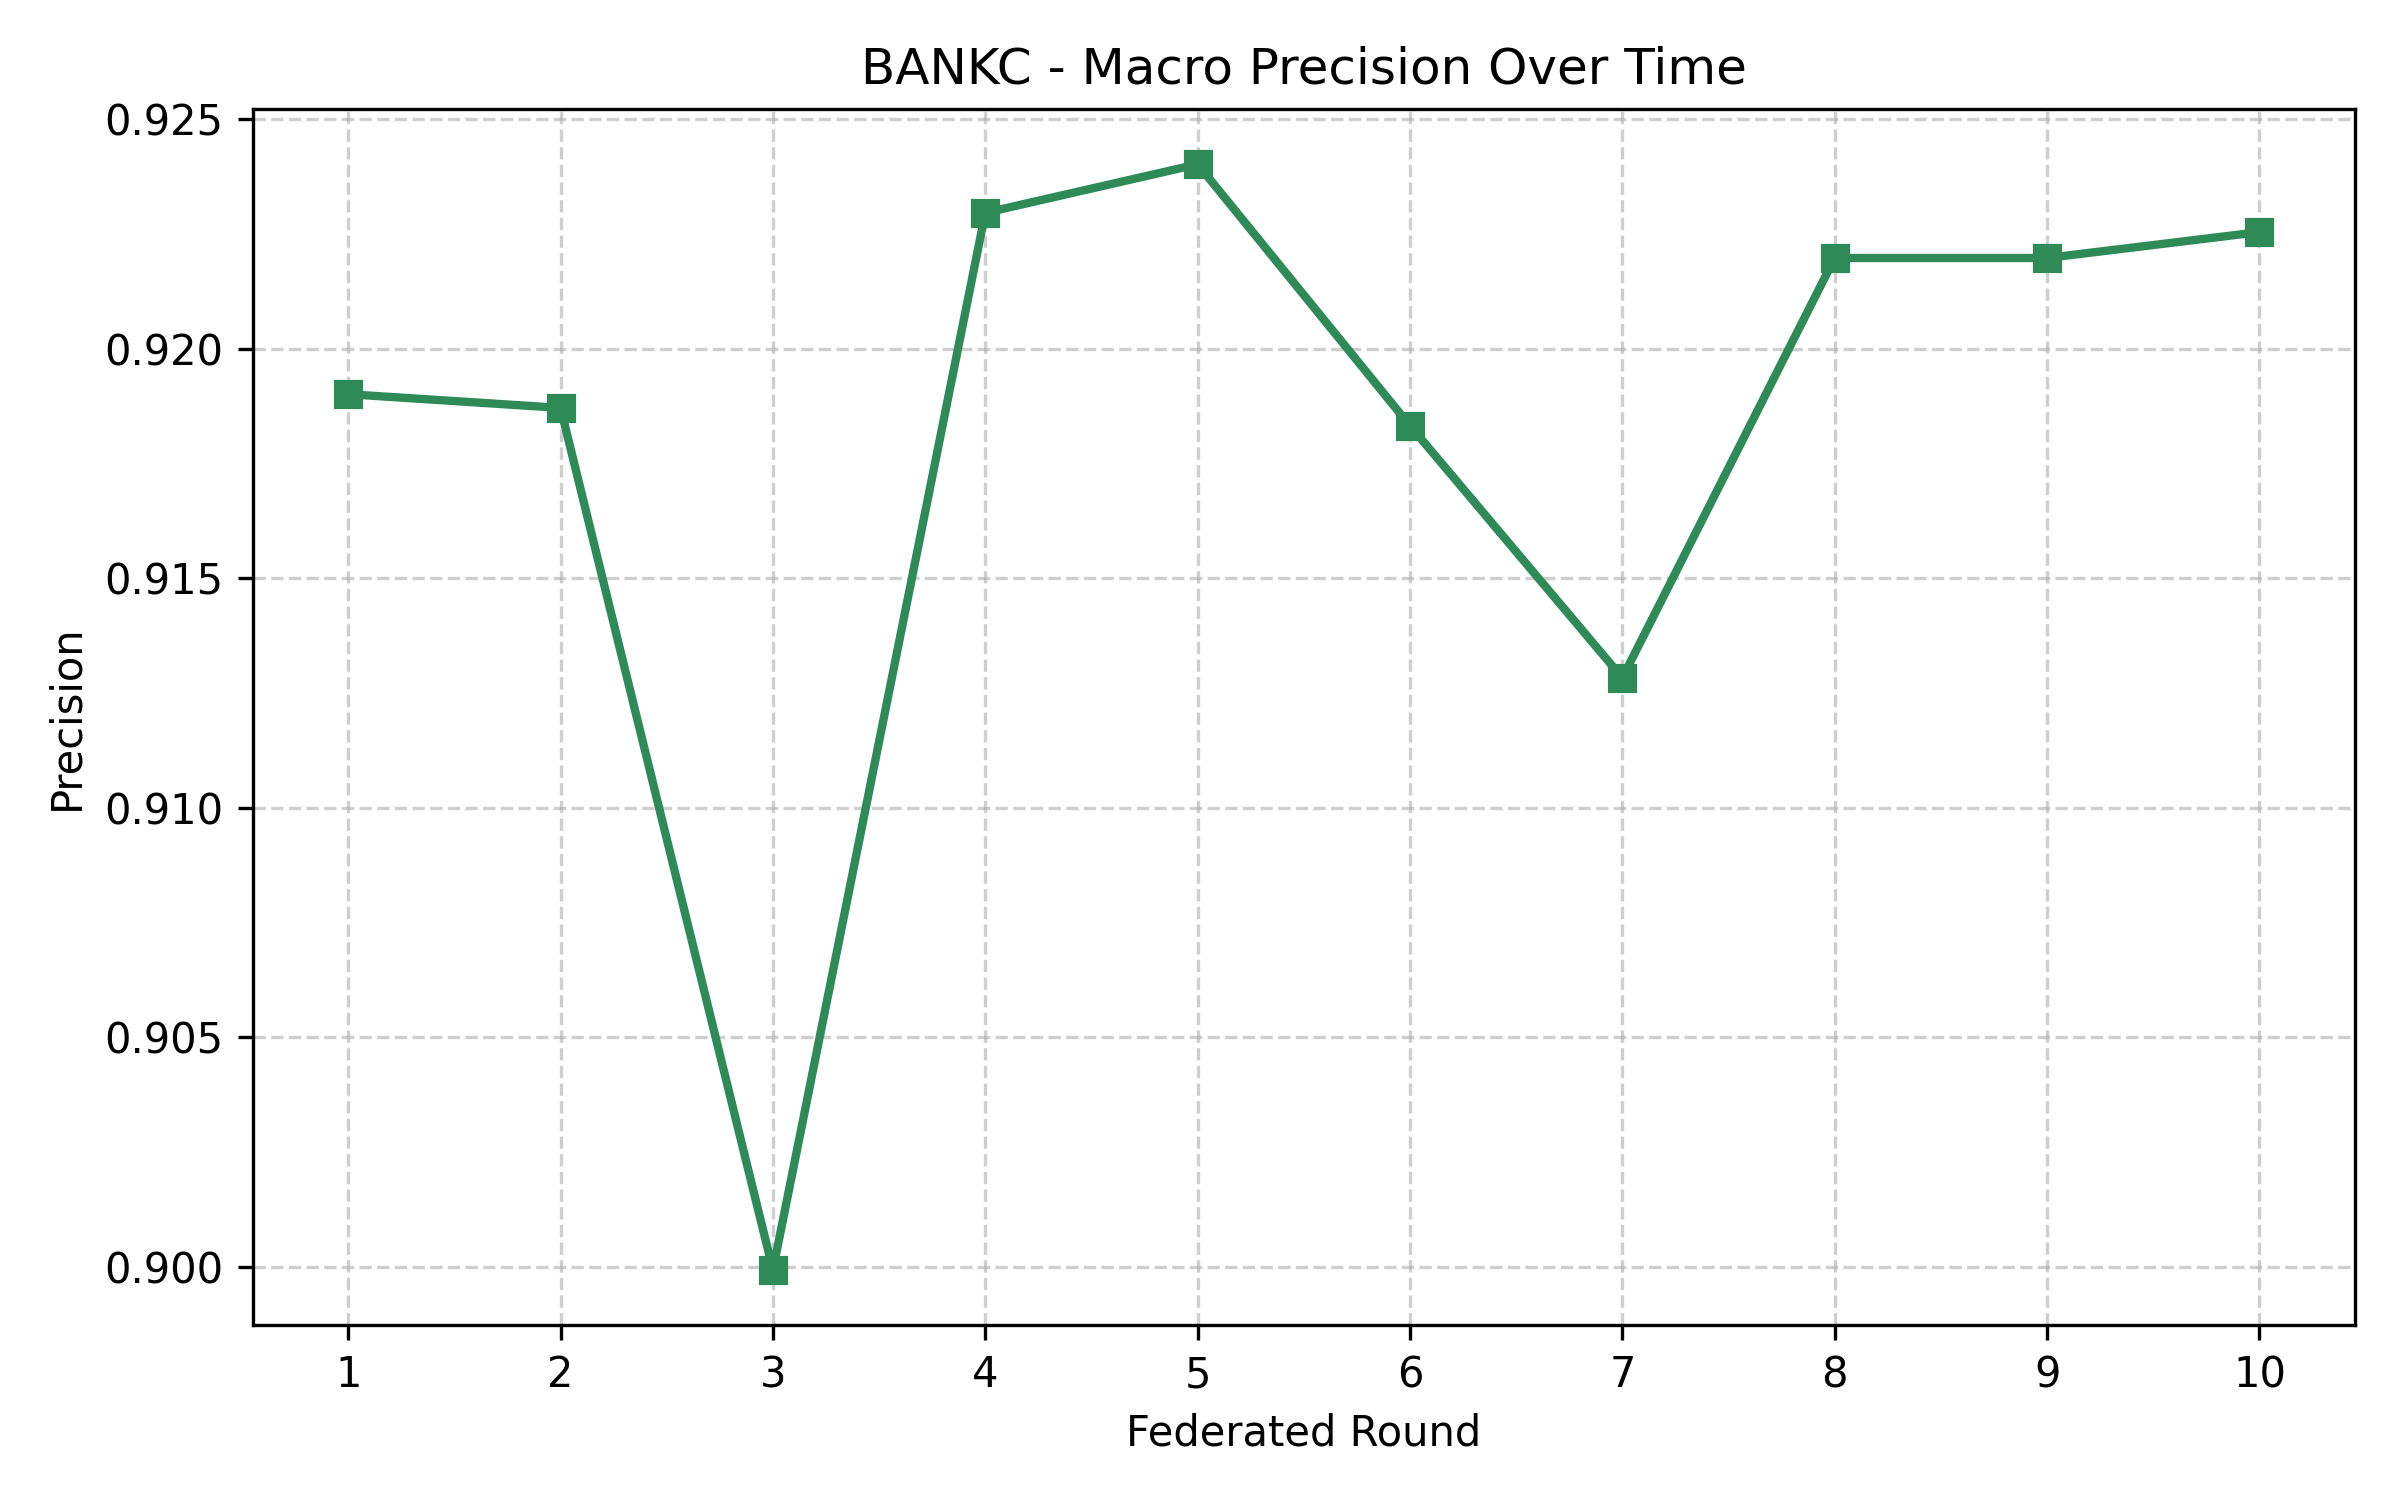
\includegraphics[width=\linewidth]{Figures/bankc_progression_precision.png}
\end{minipage}
\hfill
\begin{minipage}{0.32\textwidth}
\centering
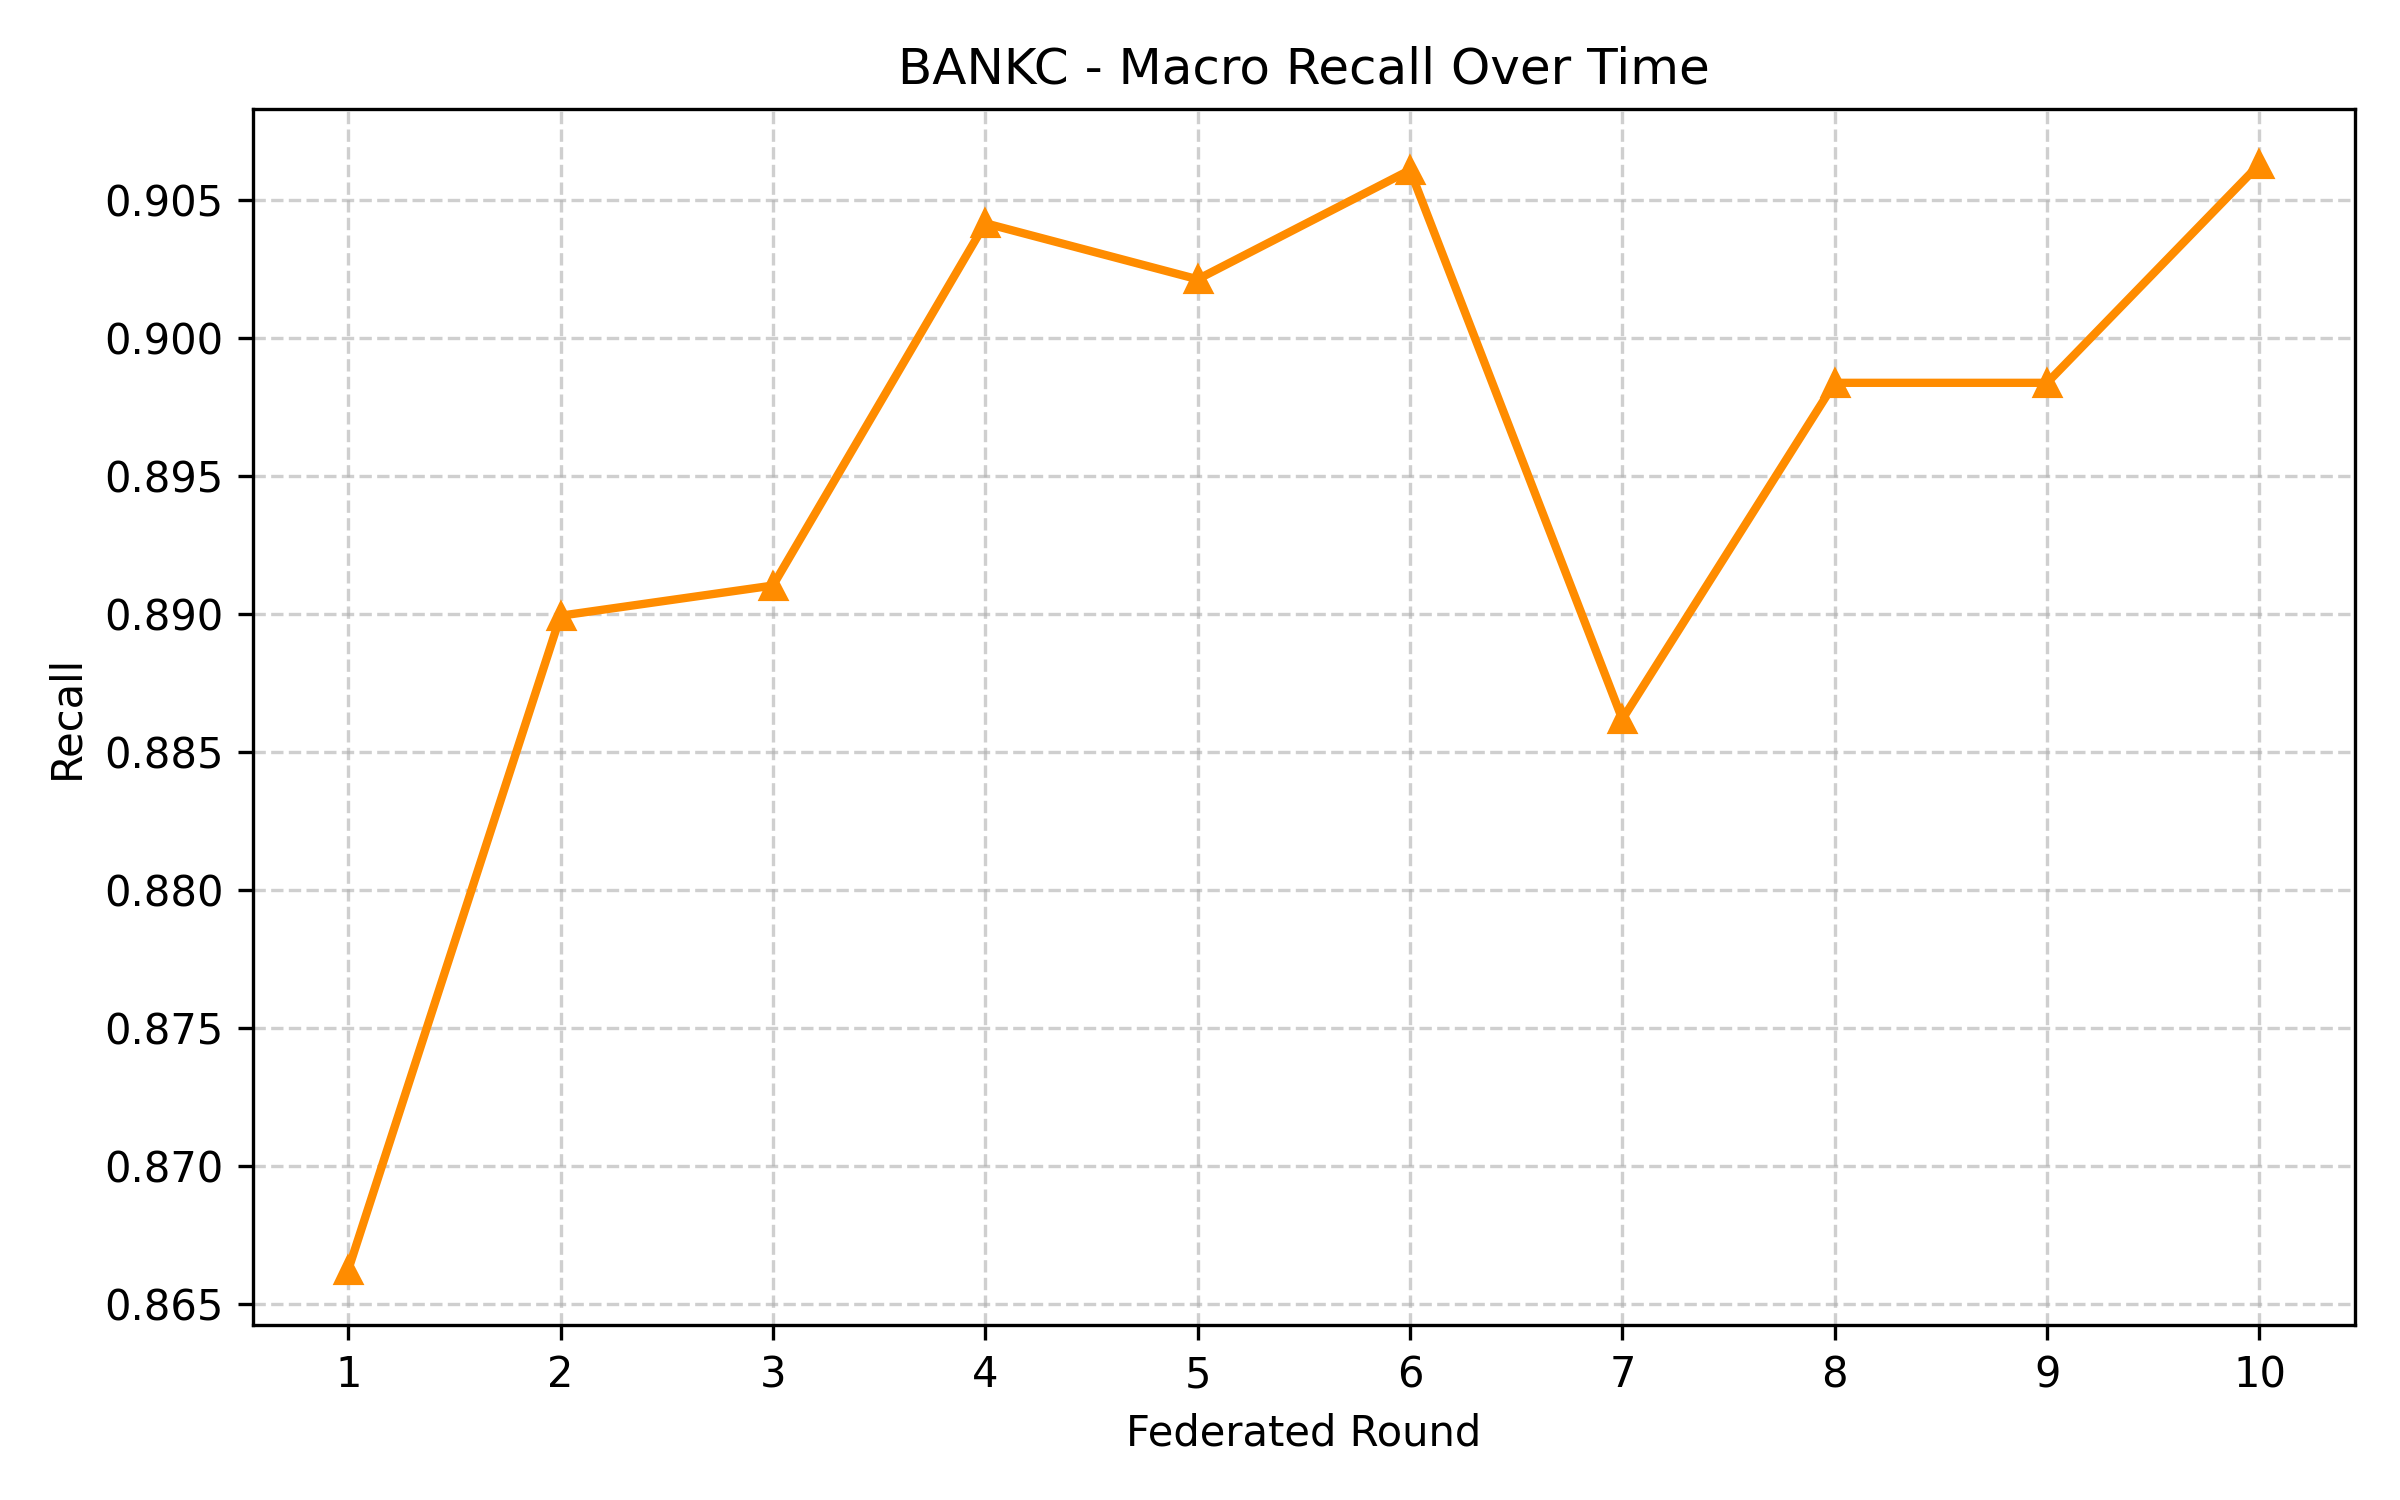
\includegraphics[width=\linewidth]{Figures/bankc_progression_recall.png}
\end{minipage}

\caption{BANKC Federated Accuracy, Precision, and Recall Progression Across Federated Aggregation Rounds}
\label{fig:bankc_progression}
\end{figure}

As shown in Figure~\ref{fig:bankc_progression}, BANKC also converged in a stable and controlled way across the full set of communication rounds. The Accuracy, Precision, and Recall values settled into a consistent range with very little movement in the later stages, which suggests that synchronization was efficient and that the distributed optimization process remained stable. It also indicates that the global model generalized well across different institutional transaction settings.
%========================================================
\subsubsection[Precision--Recall and Confusion Matrix Validation]{\textbf{Precision--Recall and Confusion Matrix Validation}}
%========================================================

Precision--Recall analysis and confusion-matrix evaluation were used to examine how well the framework separated fraud from legitimate activity, especially for the minority classes where the risk of false positives is higher. Since fraudulent transactions represented only a small portion of the full dataset, Precision--Recall gave a clearer picture of model behavior than accuracy alone.

%--------------------------------------------------------
\subsubsection{BANKA Precision--Recall and Confusion Matrix Validation}
%--------------------------------------------------------

\begin{figure}[H]
\centering

\begin{minipage}{0.48\textwidth}
\centering
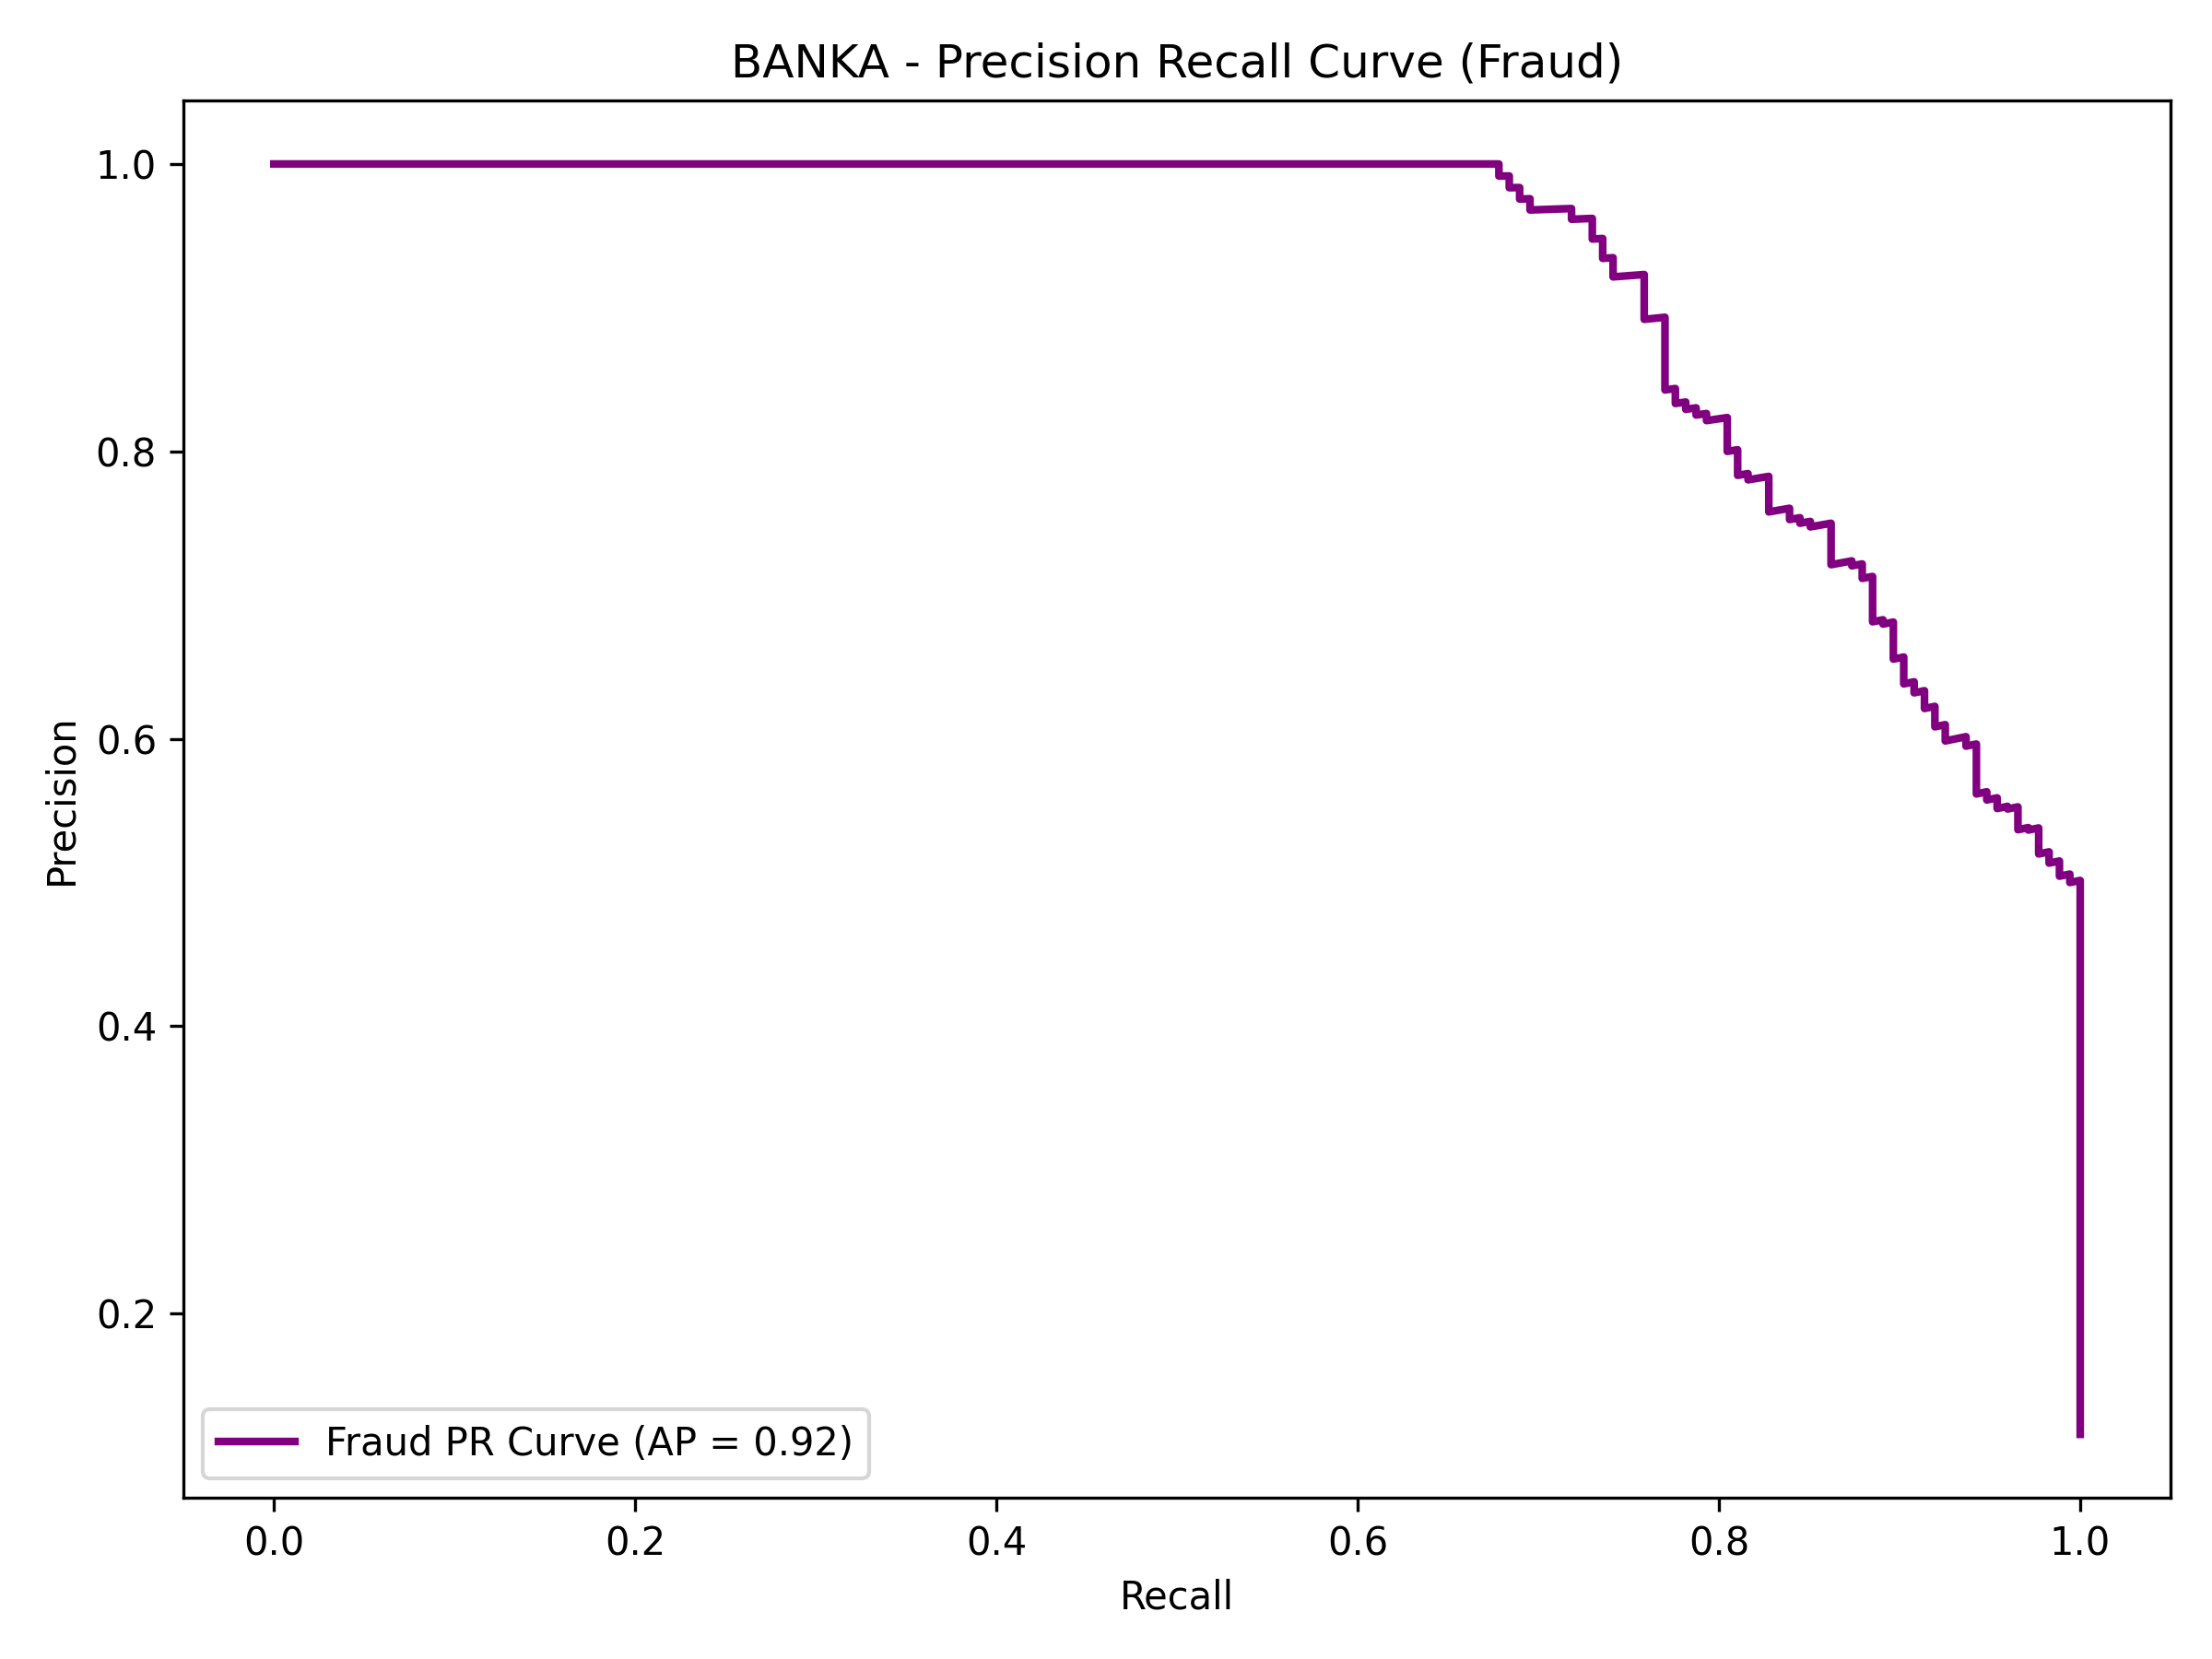
\includegraphics[width=\linewidth]{Figures/banka_pr_curve_deep.png}
\end{minipage}
\hfill
\begin{minipage}{0.48\textwidth}
\centering
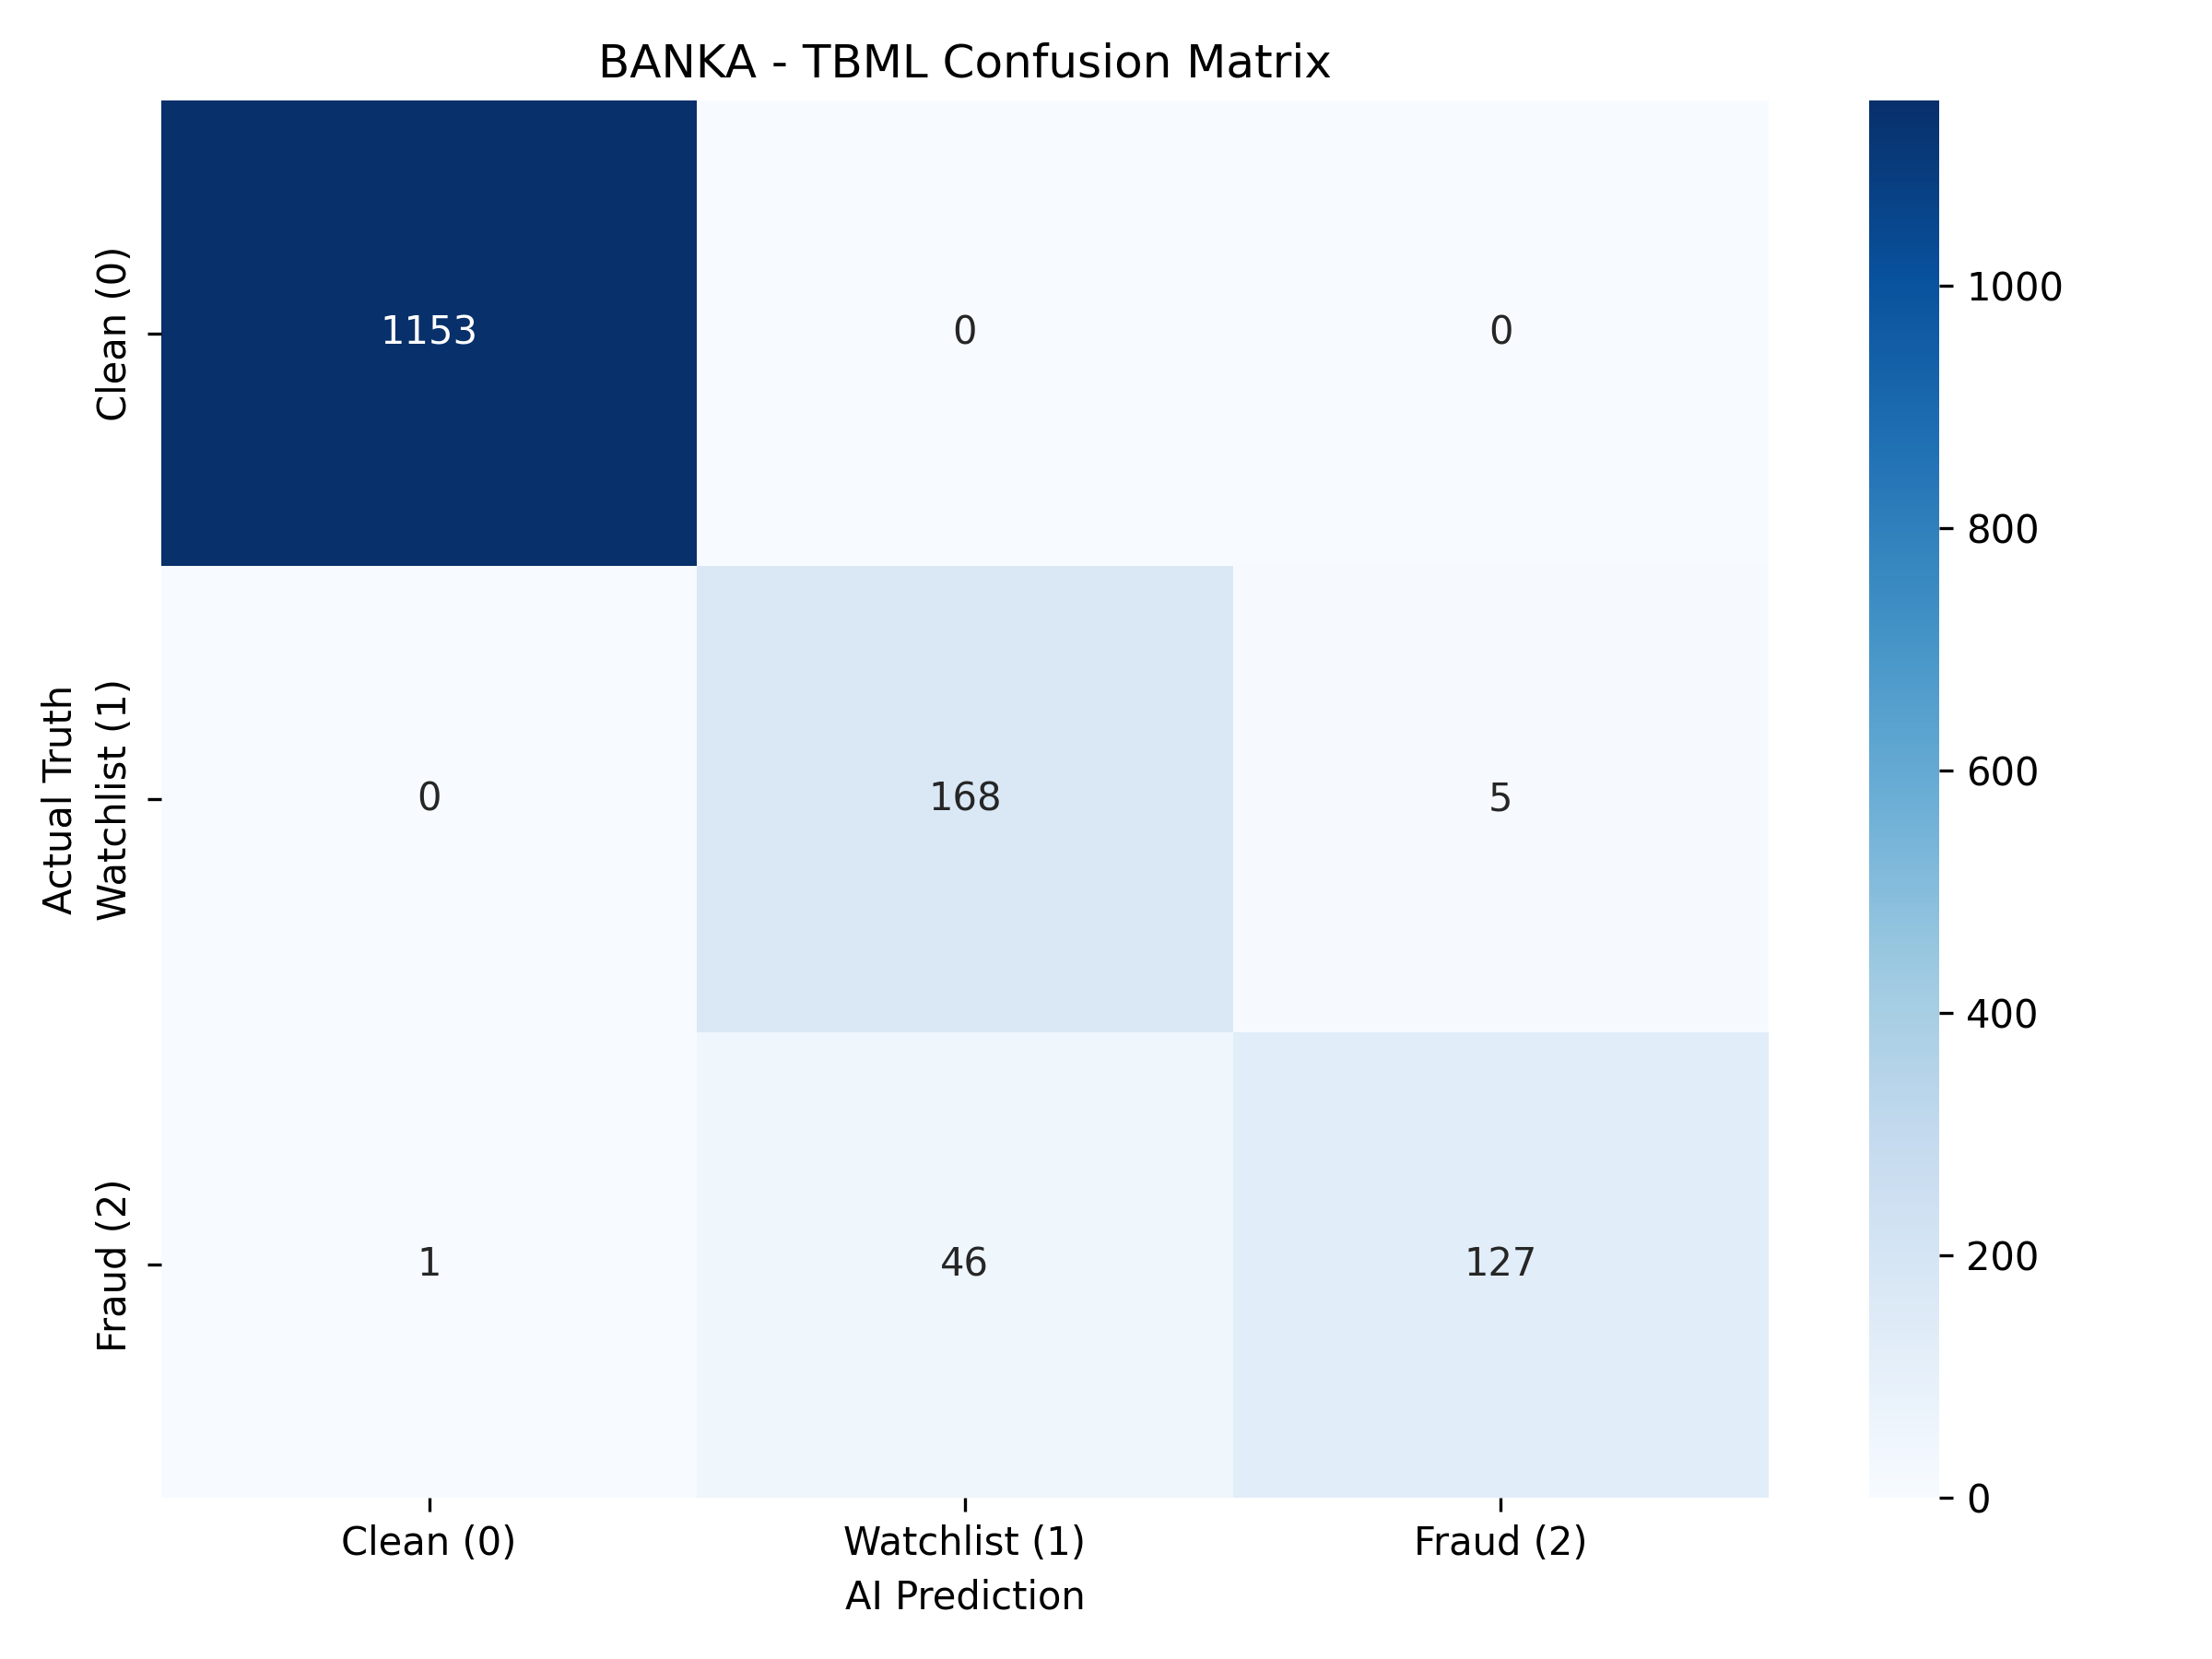
\includegraphics[width=\linewidth]{Figures/banka_confusion_matrix_deep.png}
\end{minipage}

\caption{BANKA Precision--Recall Curve and Confusion Matrix Validation}
\label{fig:banka_validation}
\end{figure}

As shown in Figure~\ref{fig:banka_validation}, BANKA achieved strong Precision--Recall performance, with Average Precision above 0.90. The curve stayed stable even as recall increased, which shows that suspicious activity was still identified reliably under an imbalanced fraud distribution. The confusion matrix also showed near-perfect classification of legitimate transactions, with very little clean-to-fraud confusion. Most overlap appeared between Watchlist and Fraud, which suggests that the model learned the subtle boundary between those two risky states without producing too many false alarms.
%--------------------------------------------------------
\subsubsection{BANKB Precision--Recall and Confusion Matrix Validation}
%--------------------------------------------------------

\begin{figure}[H]
\centering

\begin{minipage}{0.48\textwidth}
\centering
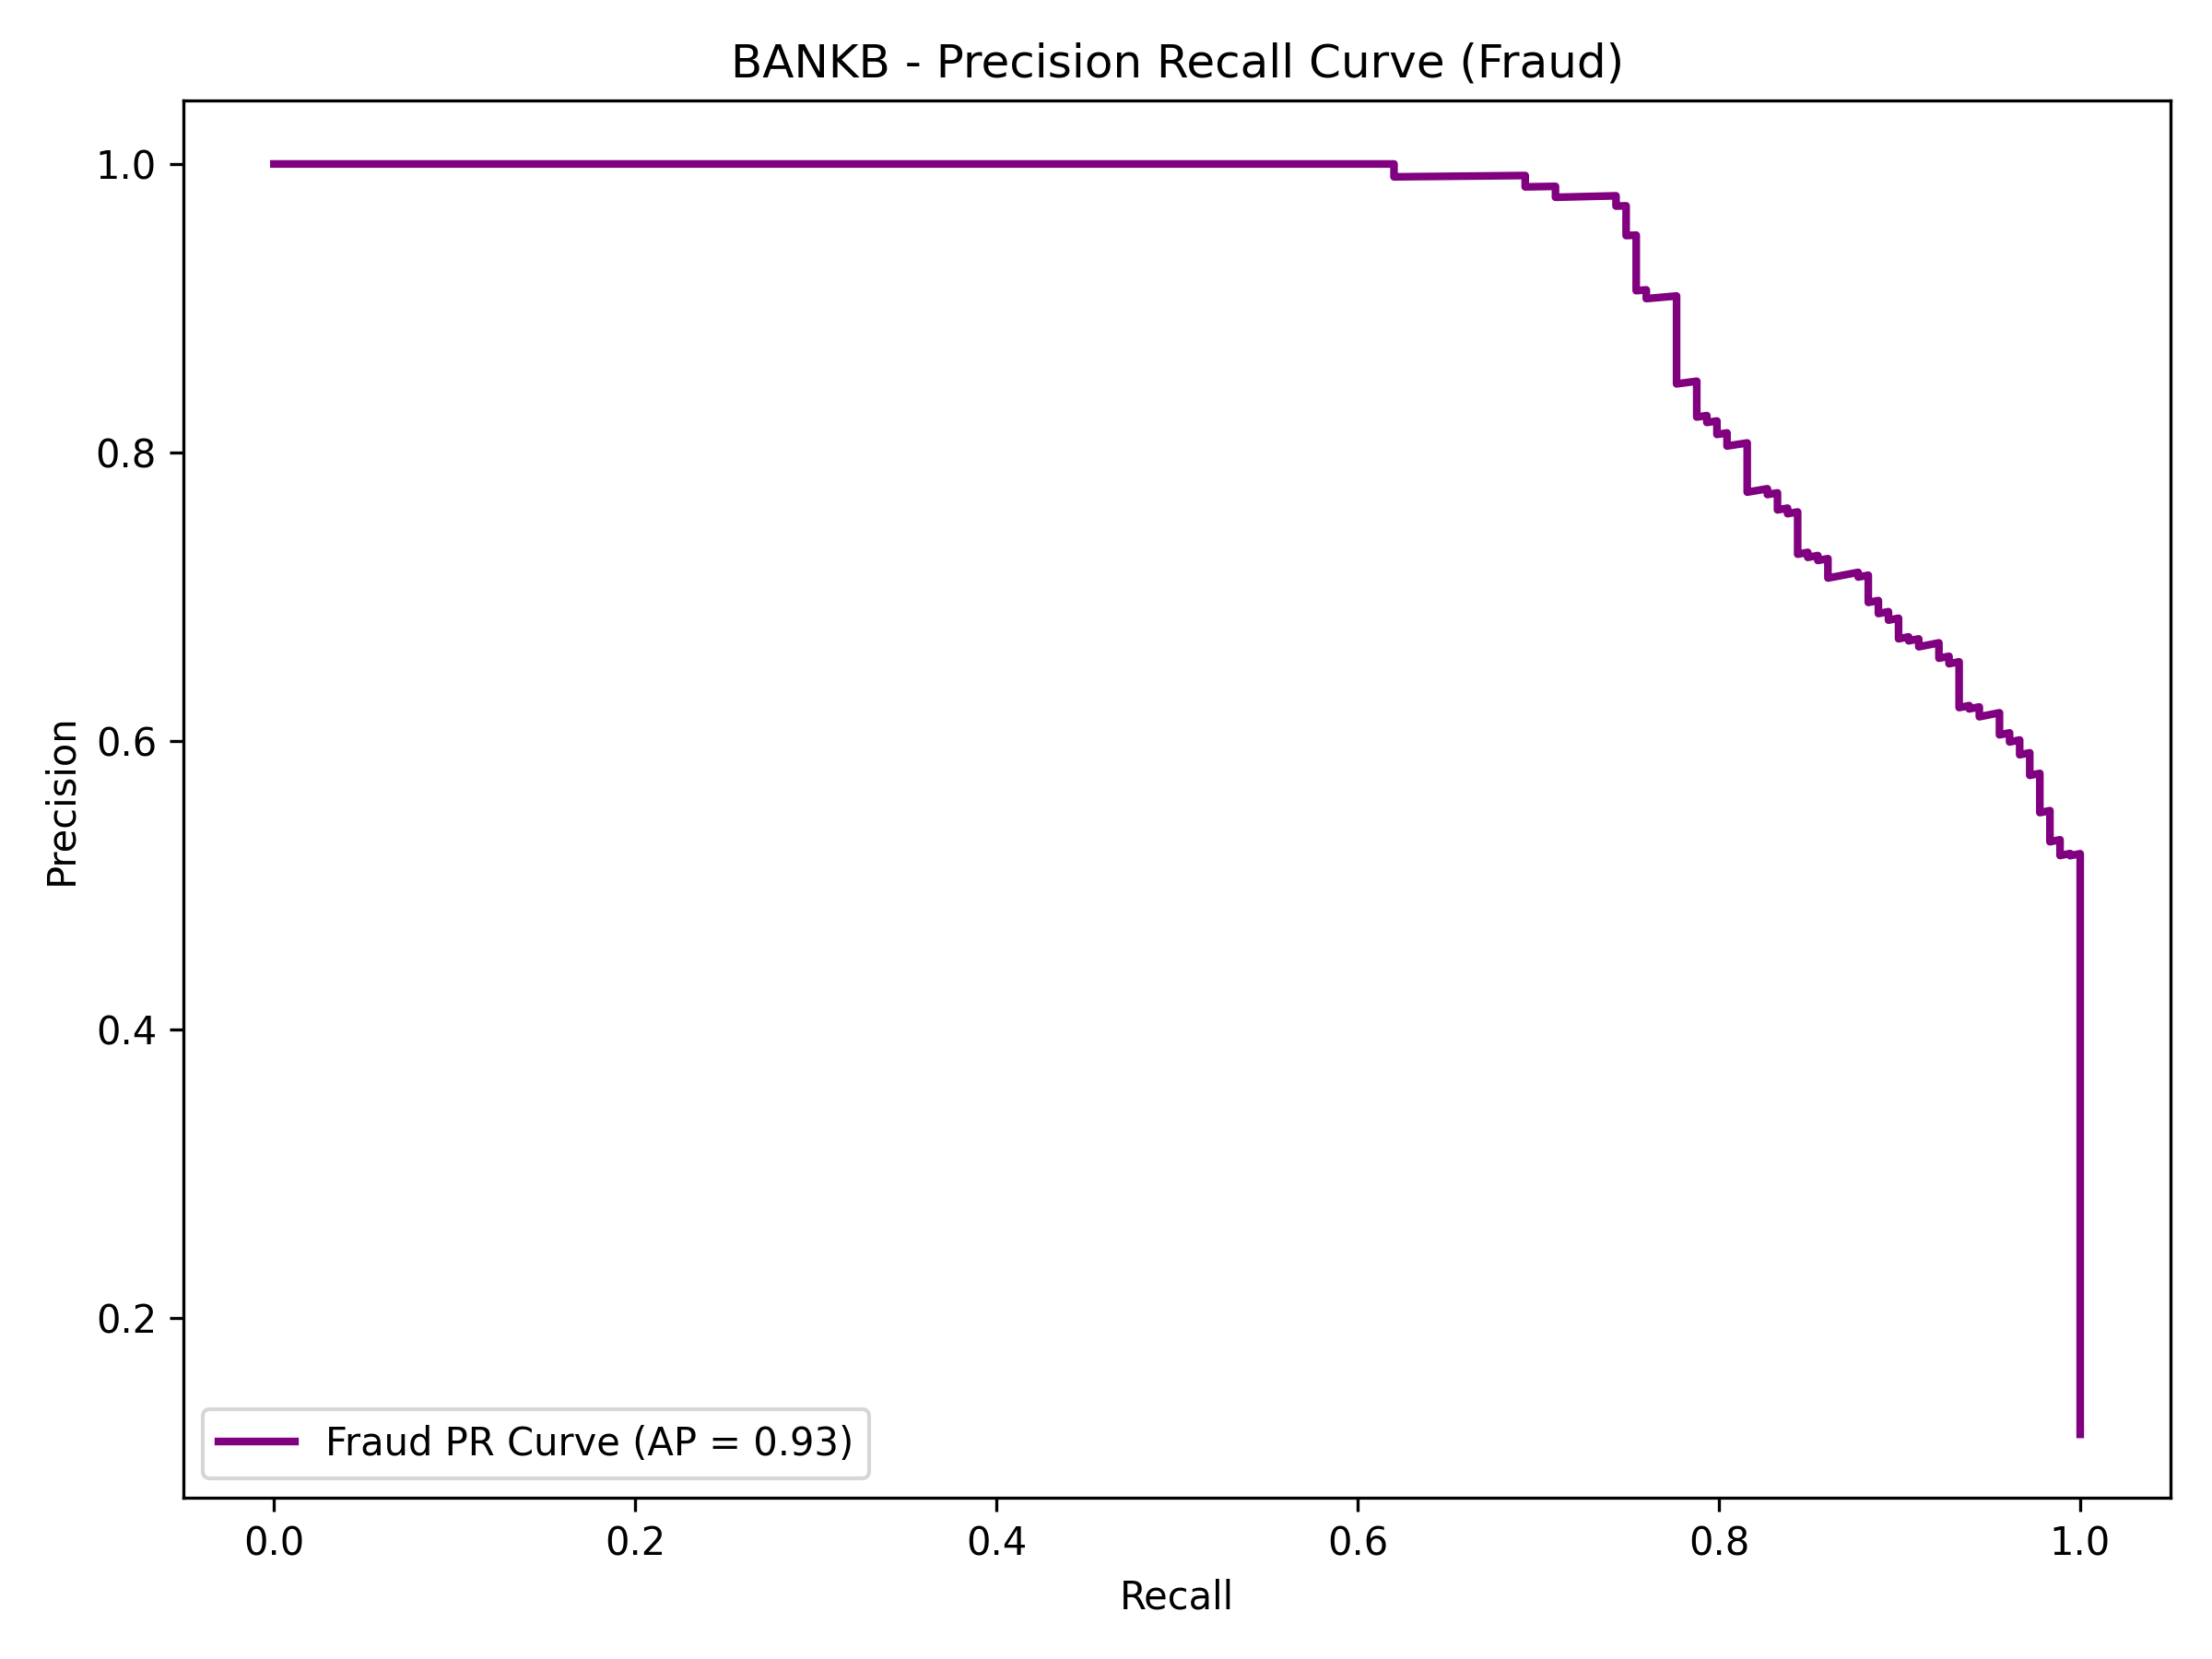
\includegraphics[width=\linewidth]{Figures/bankb_pr_curve_deep.png}
\end{minipage}
\hfill
\begin{minipage}{0.48\textwidth}
\centering
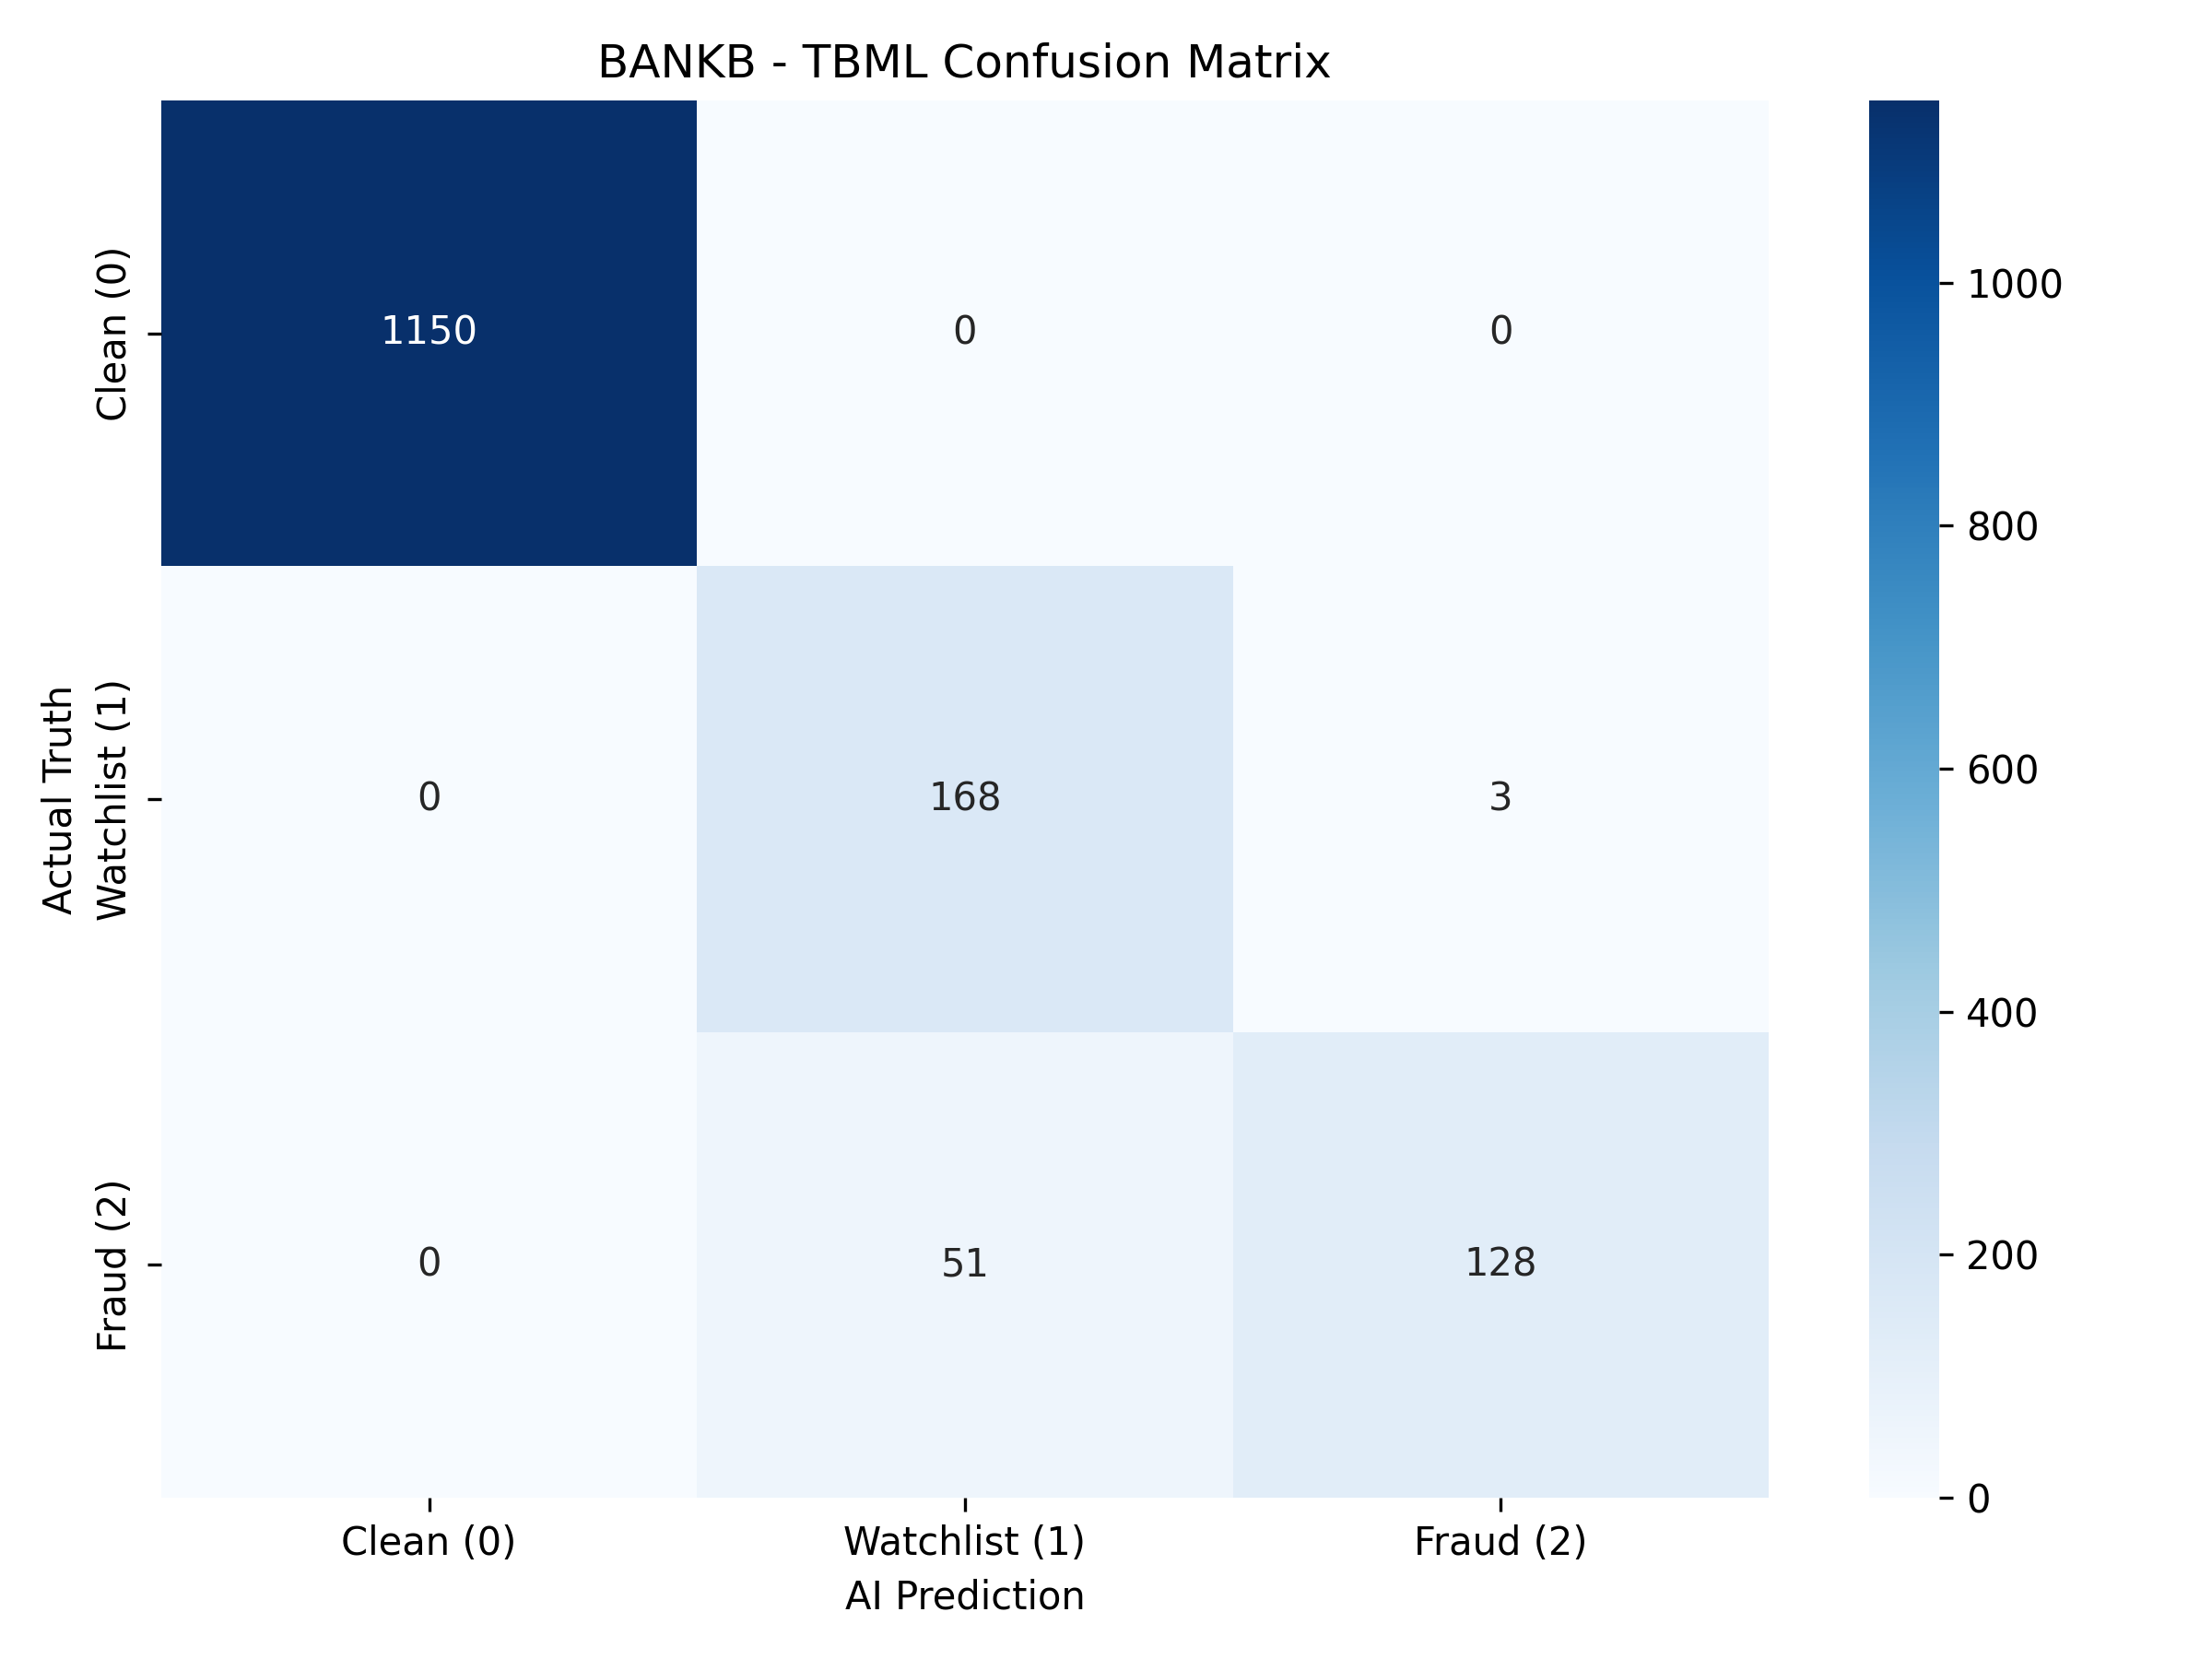
\includegraphics[width=\linewidth]{Figures/bankb_confusion_matrix_deep.png}
\end{minipage}

\caption{BANKB Precision--Recall Curve and Confusion Matrix Validation}
\label{fig:bankb_validation}
\end{figure}

As shown in Figure~\ref{fig:bankb_validation}, BANKB also delivered stable Precision--Recall behavior, again with Average Precision above 0.90. Precision stayed strong as recall increased, which confirms that the model remained sensitive to fraud without losing control over false positives. The confusion matrix showed that legitimate transactions were classified cleanly, and only a small number of Fraud cases were mapped to Watchlist, which indicates solid high-risk discrimination during monitoring.
%--------------------------------------------------------
\subsubsection{BANKC Precision--Recall and Confusion Matrix Validation}
%--------------------------------------------------------

\begin{figure}[H]
\centering

\begin{minipage}{0.48\textwidth}
\centering
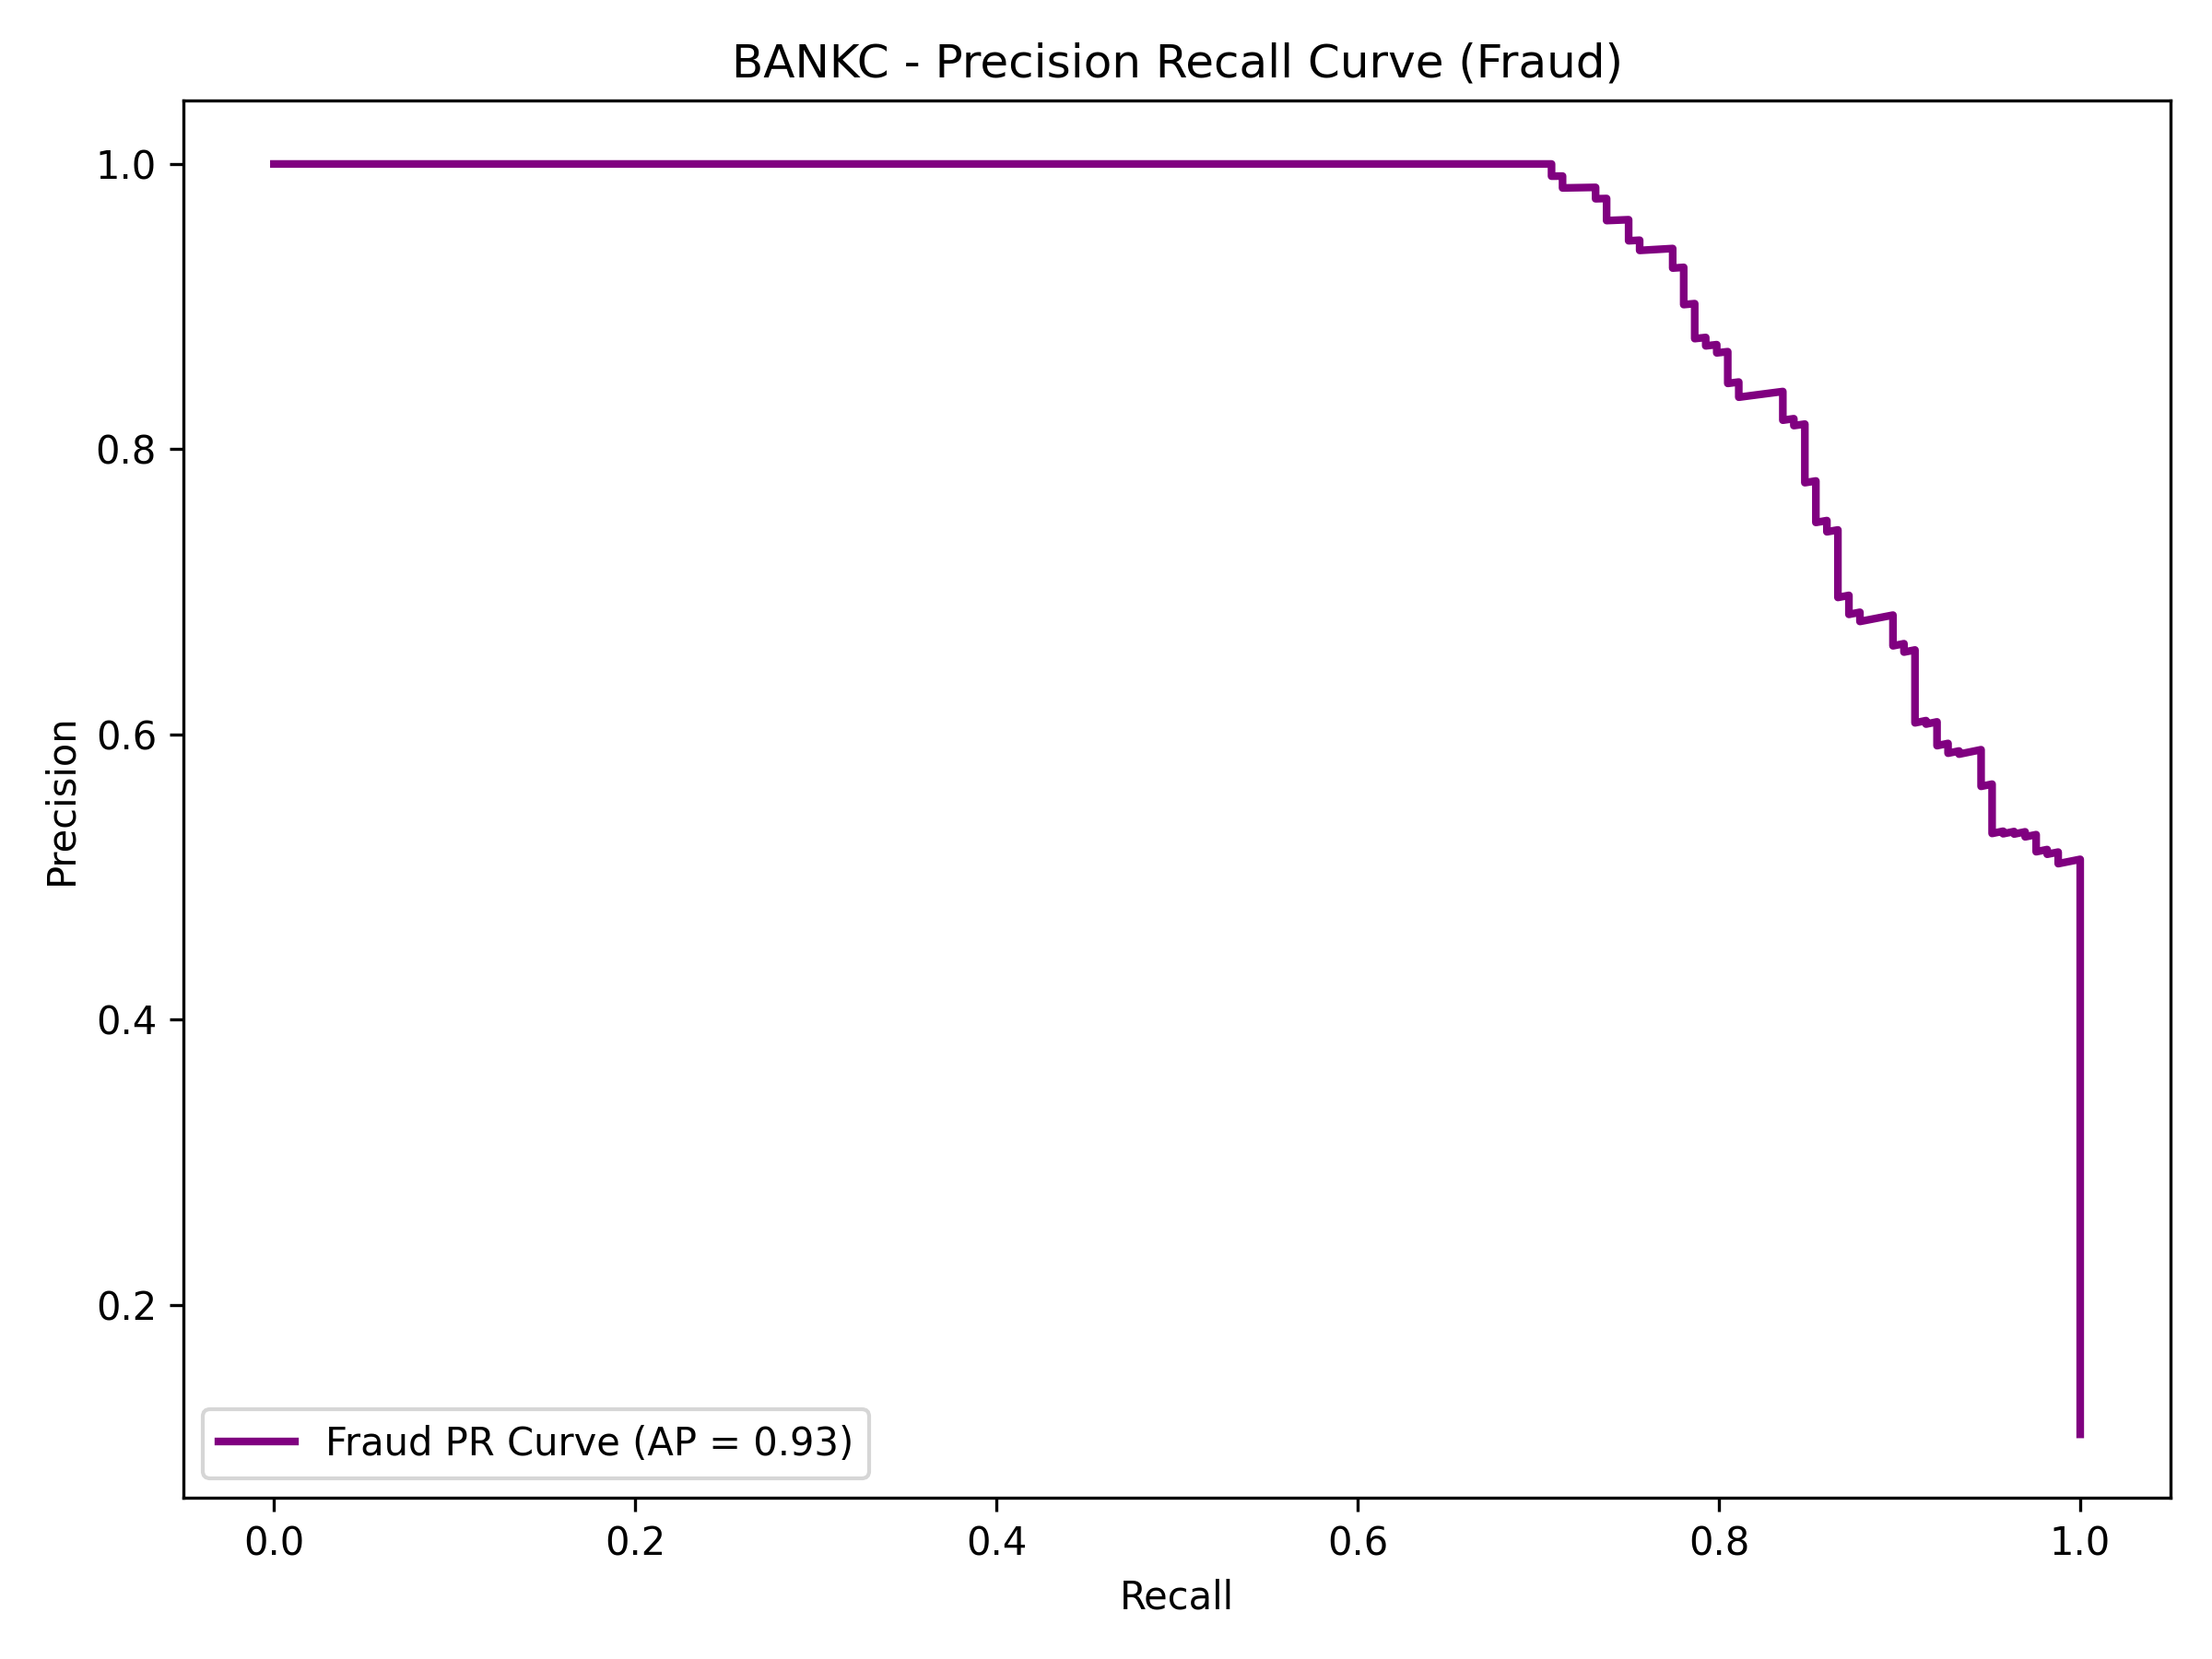
\includegraphics[width=\linewidth]{Figures/bankc_pr_curve_deep.png}
\end{minipage}
\hfill
\begin{minipage}{0.48\textwidth}
\centering
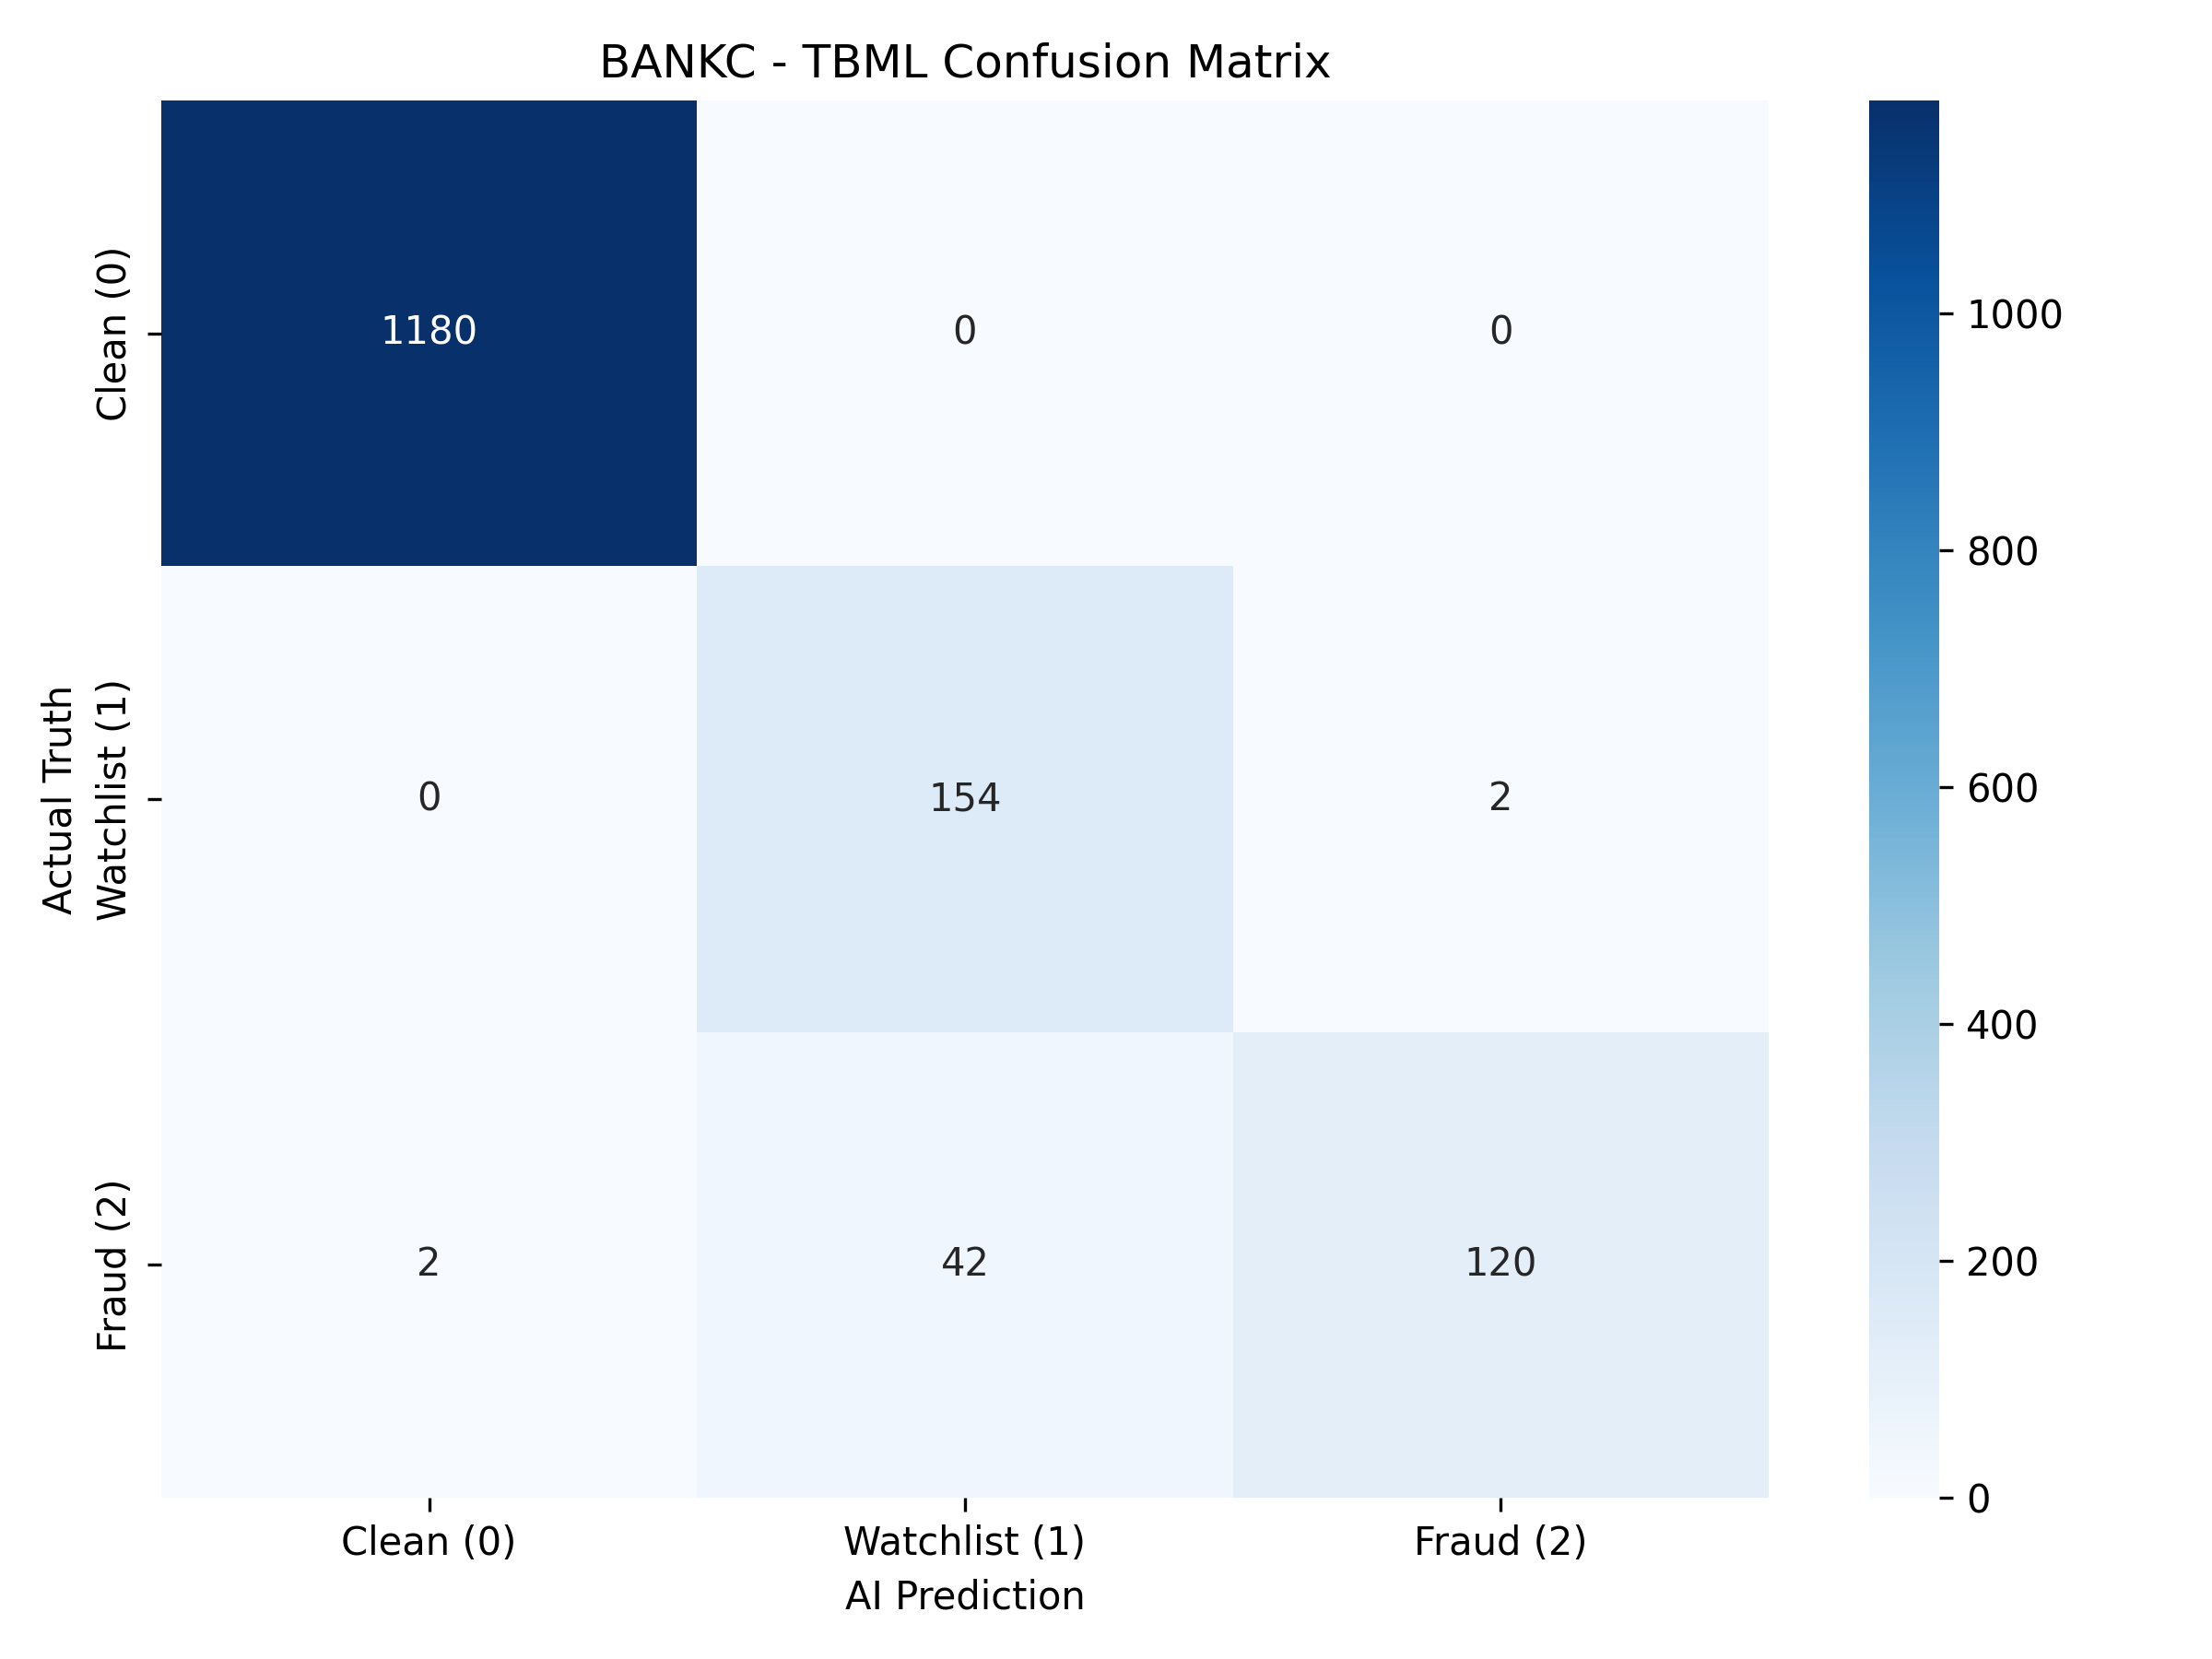
\includegraphics[width=\linewidth]{Figures/bankc_confusion_matrix_deep.png}
\end{minipage}

\caption{BANKC Precision--Recall Curve and Confusion Matrix Validation}
\label{fig:bankc_validation}
\end{figure}

As shown in Figure~\ref{fig:bankc_validation}, BANKC achieved similarly stable Precision--Recall performance, with Average Precision approaching 0.93. The curve remained steady even at higher recall levels, which points to dependable fraud detection under an imbalanced transaction distribution. The confusion matrix again showed strong consistency for legitimate transactions and very little false-positive spillover into the clean class. Most of the overlap stayed between Watchlist and Fraud, which confirms that the federated model generalized well across isolated institutional datasets.

%========================================================
\section{Summary}
%========================================================
The conducted testing and evaluation workflows validated the operational stability, synchronization reliability, and analytical performance of the proposed TBML detection framework across distributed institutional monitoring environments. The testing results confirmed stable backend communication, reliable transactional synchronization, controlled API response behavior, and successful workflow execution across graph-processing, federated analytical inference, dashboard synchronization, and compliance-management services. Concurrent scalability validation additionally demonstrated stable PostgreSQL query execution and controlled latency characteristics under increasing institutional workloads. The model performance evaluation further validated strong multi-class classification capability, stable federated convergence behavior, and reliable fraud-discrimination performance across heterogeneous institutional transaction environments without requiring centralized sharing of sensitive financial datasets.

		% % % %Chapter 7
		%========================================================
\chapter[Software Testing]{\textbf{Software Testing}}
%========================================================

In this chapter, software testing and validation techniques performed on the proposed TBML
detection framework are discussed. This includes backend analytics, transaction processing pipelines, graph construction techniques in heterogeneous environments, federated
synchronization, dashboard compliance monitoring, authentication techniques, and institutional investigation operations. In particular, this chapter describes the testing workflow
conducted in the developed software system that ensures the correct operation and synchronization within the proposed analytical system.

%========================================================
\section[Testing Environment]{\textbf{Testing Environment}}
%========================================================

The testing process was conducted in a controlled development environment consisting of Python 3.11, PyTorch, PyTorch Geometric, Apache Kafka, Memgraph, PostgreSQL, and Flower federated learning services operating within isolated virtual environments created using \texttt{venv}. Frontend monitoring interfaces were implemented and validated using Next.js, TypeScript, Tailwind CSS, Prisma ORM, Zustand state management, and JWT-based authentication workflows.

The testing workflow additionally utilized Playwright-based browser automation for validating protected dashboard routes, institutional transaction workflows, STR generation pipelines, and compliance-monitoring interfaces. Database synchronization latency, transaction propagation consistency, backend API communication, and distributed fraud-inference workflows were validated under controlled institutional transaction loads to ensure reliable execution across distributed analytical environments.

%========================================================
\section[Unit Testing]{\textbf{Unit Testing}}
%========================================================

Each backend analytical service, dashboard workflow, authentication mechanism, and database synchronization component was independently tested to validate correctness, boundary handling, synchronization stability, and operational consistency before integration into the complete TBML detection framework.
%========================================================
\subsection[Unit Testing of Authentication and RBAC Module]{\textbf{Unit Testing of Authentication and RBAC Module}}
%========================================================

The authentication and role-based access control environment was independently validated to ensure secure user authentication, authorization management, middleware-driven route protection, credential verification, and institutional role isolation across banking and regulatory dashboard interfaces. The testing workflow additionally verified protected API access, invalid credential handling, unauthorized route restrictions, and role-specific dashboard rendering across distributed monitoring environments.
\renewcommand{\arraystretch}{1.3}

\begin{table}[H]
\centering
\caption{TC-001: Unit Testing of Authentication and RBAC Module}
\label{tab:auth_rbac_test}
\vspace{0.2cm}
\begin{tabular}{|p{4.2cm}|p{9cm}|}
\hline
\textbf{Serial Number of Test Case} & TC-001 \\ \hline
\textbf{Name of Test Case} & Protected Dashboard Access Validation \\ \hline
\textbf{Feature being Tested} & Authentication and Authorization Validation \\ \hline
\textbf{Description} & Validate protected route access, JWT verification, and role-based authorization \\ \hline
\textbf{Sample Input} & Invalid JWT session and unauthorized user request \\ \hline
\textbf{Expected Output} & Unauthorized access denied with authentication error response \\ \hline
\textbf{Actual Output} & Invalid sessions blocked and unauthorized users redirected successfully \\ \hline
\textbf{Remarks} & Successful test \\ \hline
\end{tabular}
\end{table}

As shown in Table~\ref{tab:auth_rbac_test}, middleware-driven session validation successfully enforced protected route isolation and role-specific dashboard authorization across institutional monitoring environments. The testing workflow validated JWT token verification, session-expiration handling, credential validation, protected API access control, and middleware-based authorization checks across banking and regulator dashboards. Invalid credentials, unauthorized API requests, expired authentication sessions, and direct access attempts to protected routes were correctly rejected using backend access-control policies before protected resources were rendered. The authentication workflow additionally verified successful role mapping for \texttt{BANK\_USER} and \texttt{ADMIN} entities to ensure secure dashboard isolation and controlled access to institutional fraud-monitoring operations.
%========================================================
\subsection[Unit Testing of Kafka Transaction Streaming]{\textbf{Unit Testing of Kafka Transaction Streaming}}
%========================================================

The Kafka transaction streaming environment was independently tested to validate asynchronous transaction publishing, real-time event synchronization, payload integrity validation, and downstream analytical communication across distributed backend services. The testing workflow additionally verified message delivery consistency, topic-based transaction propagation, malformed payload handling, and reliable synchronization between Kafka producer and consumer services operating within the proposed framework.


\begin{table}[H]
\centering
\caption{TC-002: Unit Testing of Kafka Transaction Streaming}
\label{tab:kafka_test}
\vspace{0.2cm}

\begin{tabular}{|p{4.2cm}|p{9cm}|}
\hline
\textbf{Serial Number of Test Case} & TC-002 \\ \hline
\textbf{Name of Test Case} & Publish Valid SWIFT Transaction \\ \hline
\textbf{Feature being Tested} & Kafka Event Streaming and Message Synchronization \\ \hline
\textbf{Description} & Validate transaction publishing and topic-based event synchronization \\ \hline
\textbf{Sample Input} & JSON transaction payload containing sender, receiver, amount, and trade metadata \\ \hline
\textbf{Expected Output} & Transaction published into \texttt{incoming\_swift\_messages} topic successfully \\ \hline
\textbf{Actual Output} & Transaction streamed and synchronized successfully across Kafka services \\ \hline
\textbf{Remarks} & Successful test \\ \hline
\end{tabular}
\end{table}

As shown in Table~\ref{tab:kafka_test}, the Kafka streaming module successfully validated asynchronous transaction publishing and backend event synchronization across distributed analytical services. Producer and consumer services maintained reliable message propagation and transaction consistency during continuous event-stream processing operations. Invalid payload structures, malformed transaction metadata, and incomplete financial events were correctly rejected through backend validation workflows before downstream graph-processing and fraud-inference operations were initiated.

%========================================================
\subsection[Unit Testing of Graph Construction Module]{\textbf{Unit Testing of Graph Construction Module}}
%========================================================

The heterogeneous graph-construction environment was independently tested to validate transactional node generation, relationship mapping, multi-entity graph synchronization, and Cypher-based ingestion workflows within the Memgraph analytical environment. The testing workflow additionally verified graph consistency, entity-link generation, transaction propagation accuracy, and downstream graph availability for Hybrid HGNN--LSTM analytical inference operations.

\begin{table}[H]
\centering
\caption{TC-003: Unit Testing of Graph Construction Module}
\label{tab:graph_construction_test}
\vspace{0.2cm}

\begin{tabular}{|p{4.2cm}|p{9cm}|}
\hline
\textbf{Serial Number of Test Case} & TC-003 \\ \hline
\textbf{Name of Test Case} & Heterogeneous Graph Entity Generation \\ \hline
\textbf{Feature being Tested} & Memgraph Graph Construction and Relationship Mapping \\ \hline
\textbf{Description} & Validate transactional node generation and graph relationship synchronization \\ \hline
\textbf{Sample Input} & Valid SWIFT transaction payload with account, trade, and document metadata \\ \hline
\textbf{Expected Output} & Graph nodes and transactional relationships created successfully within Memgraph \\ \hline
\textbf{Actual Output} & Heterogeneous graph entities and multi-hop relationships generated successfully \\ \hline
\textbf{Remarks} & Successful test \\ \hline
\end{tabular}
\end{table}

As shown in Table~\ref{tab:graph_construction_test}, the graph-construction workflow successfully generated heterogeneous transactional graphs within the Memgraph environment using Cypher-based ingestion and relationship-mapping operations. Graph entities including \texttt{(:Account)}, \texttt{(:Transaction)}, and \texttt{(:Document)} were correctly synchronized with transactional relationships such as \texttt{[:SENDS]}, \texttt{[:TO]}, and \texttt{[:HAS\_DOC]} during continuous event-stream processing. The testing workflow additionally validated graph consistency, entity-link integrity, and multi-hop transactional connectivity required for downstream subgraph extraction and graph-based fraud inference operations within the proposed framework.

%========================================================
\subsection[Unit Testing of STR Generation Workflow]{\textbf{Unit Testing of STR Generation Workflow}}
%========================================================

The STR generation workflow was independently tested to validate suspicious transaction report generation, compliance-record synchronization, fraud-case escalation, and regulator-side notification propagation across distributed institutional monitoring environments. The testing workflow additionally verified report persistence, transaction-metadata preservation, audit consistency, and downstream synchronization between banking dashboards and regulator-facing compliance interfaces.


\begin{table}[H]
\centering
\caption{TC-004: Unit Testing of STR Generation Workflow}
\label{tab:str_generation_test}
\vspace{0.2cm}

\begin{tabular}{|p{4.2cm}|p{9cm}|}
\hline
\textbf{Serial Number of Test Case} & TC-004 \\ \hline
\textbf{Name of Test Case} & Suspicious Transaction Report Generation \\ \hline
\textbf{Feature being Tested} & STR Generation and Compliance Synchronization \\ \hline
\textbf{Description} & Validate fraud escalation and regulator-side STR synchronization workflow \\ \hline
\textbf{Sample Input} & Fraud-classified transaction selected from institutional monitoring dashboard \\ \hline
\textbf{Expected Output} & STR record generated and synchronized into regulator compliance environment \\ \hline
\textbf{Actual Output} & STR generated, persisted, and synchronized successfully across monitoring services \\ \hline
\textbf{Remarks} & Successful test \\ \hline
\end{tabular}
\end{table}


As shown in Table~\ref{tab:str_generation_test}, the STR workflow successfully validated automated fraud-report generation, PostgreSQL audit synchronization, and regulator-side notification propagation across distributed institutional environments. Generated STR records correctly preserved transaction metadata, fraud classifications, institutional identifiers, and investigation references during downstream compliance synchronization operations. The testing workflow additionally verified successful dashboard synchronization, report persistence, and controlled propagation of suspicious transaction alerts between banking institutions and regulatory monitoring interfaces operating within the proposed framework.

%========================================================
\subsection[Unit Testing of Notification Workflow]{\textbf{Unit Testing of Notification Workflow}}
%========================================================

The notification synchronization environment was independently tested to validate fraud-alert propagation, institutional notification delivery, compliance-event synchronization, and regulator-side alert visibility across distributed monitoring interfaces. The testing workflow additionally verified notification persistence, dashboard update consistency, backend event propagation, and synchronization between banking and regulatory compliance environments during fraud escalation operations.


\begin{table}[H]
\centering
\caption{TC-005: Unit Testing of Notification Workflow}
\label{tab:notification_workflow_test}
\vspace{0.2cm}

\begin{tabular}{|p{4.2cm}|p{9cm}|}
\hline
\textbf{Serial Number of Test Case} & TC-005 \\ \hline
\textbf{Name of Test Case} & Fraud Alert and Compliance Notification Propagation \\ \hline
\textbf{Feature being Tested} & Notification Synchronization and Alert Delivery \\ \hline
\textbf{Description} & Validate fraud-alert propagation across banking and regulator monitoring environments \\ \hline
\textbf{Sample Input} & Generated STR record linked to fraud-classified transaction \\ \hline
\textbf{Expected Output} & Compliance alerts synchronized into regulator-facing dashboard interfaces \\ \hline
\textbf{Actual Output} & Fraud notifications propagated and synchronized successfully \\ \hline
\textbf{Remarks} & Successful test \\ \hline
\end{tabular}
\end{table}


As shown in Table~\ref{tab:notification_workflow_test}, he notification workflow successfully validated fraud-alert propagation, institutional investigation updates, and STR lifecycle synchronization across distributed compliance-monitoring environments. Backend event-processing services maintained reliable notification delivery and dashboard synchronization during fraud escalation operations between banking institutions and regulatory authorities. The testing workflow additionally verified notification persistence, regulator-side alert visibility, and consistent compliance-state propagation across protected monitoring interfaces operating within the proposed framework.



%========================================================
\subsection[Integration Testing]{\textbf{Integration Testing}}
%========================================================

Integration testing was conducted to validate the interaction, synchronization consistency, and workflow stability between distributed analytical services, graph-processing environments, fraud inference pipelines, dashboard-rendering systems, and regulatory compliance workflows operating within the proposed TBML detection framework.

%========================================================
\subsection[Integration Testing of Kafka and Memgraph Pipeline]{\textbf{Integration Testing of Kafka and Memgraph Pipeline}}
%========================================================

This integration test validated end-to-end synchronization between Kafka-based transaction streaming services and the heterogeneous graph-construction environment operating within Memgraph. The testing workflow additionally verified event-stream consistency, transaction propagation reliability, graph-ingestion stability, and downstream synchronization between distributed backend services.

\renewcommand{\arraystretch}{1.3}

\begin{table}[H]
\centering
\caption{TC-006: Integration Testing of Kafka and Memgraph Pipeline}
\label{tab:kafka_memgraph_integration_test}`'
\vspace{0.2cm}

\begin{tabular}{|p{4.2cm}|p{9cm}|}
\hline
\textbf{Serial Number of Test Case} & TC-006 \\ \hline
\textbf{Name of Test Case} & Transaction Stream and Graph Synchronization Workflow \\ \hline
\textbf{Feature being Tested} & Kafka Event Propagation and Memgraph Synchronization \\ \hline
\textbf{Description} & Validate transaction-stream synchronization and heterogeneous graph generation \\ \hline
\textbf{Sample Input} & Valid Kafka transaction payload with trade metadata and KYC attributes \\ \hline
\textbf{Expected Output} & Transactional graph entities and relationships generated successfully within Memgraph \\ \hline
\textbf{Actual Output} & Kafka events synchronized and heterogeneous graph generated successfully \\ \hline
\textbf{Remarks} & Successful test \\ \hline
\end{tabular}
\end{table}

\renewcommand{\arraystretch}{1}

As shown in Table~\ref{tab:kafka_memgraph_integration_test}, the integration workflow successfully validated asynchronous transaction propagation between Kafka producer-consumer services and Memgraph graph-ingestion environments. Streamed SWIFT transaction events were reliably synchronized into graph-processing pipelines without transactional inconsistency or event-loss during continuous backend processing operations. The testing workflow additionally verified stable graph synchronization, multi-entity relationship generation, and downstream availability of transactional subgraphs required for graph-based analytical inference within the proposed framework.


%========================================================
\subsection[Integration Testing of Fraud Prediction and Dashboard Synchronization]{\textbf{Integration Testing of Fraud Prediction and Dashboard Synchronization}}
%========================================================

This integration test validated synchronization between fraud-prediction services, PostgreSQL audit environments, and role-based monitoring dashboards operating within the proposed TBML framework. The testing workflow additionally verified database persistence, dashboard synchronization consistency, and real-time rendering of fraud-classified transactions.

\renewcommand{\arraystretch}{1.3}

\begin{table}[H]
\centering
\caption{TC-007: Integration Testing of Fraud Prediction and Dashboard Synchronization}
\label{tab:fraud_prediction_dashboard_integration_test}
\vspace{0.2cm}

\begin{tabular}{|p{4.2cm}|p{9cm}|}
\hline
\textbf{Serial Number of Test Case} & TC-007 \\ \hline
\textbf{Name of Test Case} & Fraud Prediction and Dashboard Rendering Workflow \\ \hline
\textbf{Feature being Tested} & PostgreSQL Synchronization and Dashboard Visualization \\ \hline
\textbf{Description} & Validate fraud-prediction synchronization into institutional monitoring dashboards \\ \hline
\textbf{Sample Input} & Fraud-classified transaction generated from analytical inference pipeline \\ \hline
\textbf{Expected Output} & Fraud transaction persisted and rendered successfully within dashboard interfaces \\ \hline
\textbf{Actual Output} & Dashboard synchronization completed successfully with valid fraud-state rendering \\ \hline
\textbf{Remarks} & Successful test \\ \hline
\end{tabular}
\end{table}

\renewcommand{\arraystretch}{1}

The integration test ensured proper synchronization of fraud-prediction services,
PostgreSQL audit environments, and dashboards for role-based monitoring working
under the TBML architecture. The testing process further confirmed persistence of the
database, consistency of dashboard synchronization, and rendering of fraud-classified
transactions.  Integration Testing of Fraud Prediction and Dashboard Synchronization It can be seen from Table~\ref{tab:fraud_prediction_dashboard_integration_test} that records of fraud predictions, transaction data, and
risk classifications of institutions were synchronized in centralized PostgreSQL audit
systems and then rendered using secure dashboard applications. The synchronization of the dashboards ensured proper propagation of fraud status and transaction visibility in
institutional monitoring services.


%========================================================
\subsection[Integration Testing of STR Generation Workflow]{\textbf{Integration Testing of STR Generation Workflow}}
%========================================================
This integration test confirmed the full integration from institutional fraud verification, STR generation services, regulator-side synchronization and propagation of compliance notifications in the distributed monitoring environments. The testing process also confirmed that fraud escalation is consistent, reports are persistent, and regulators are seamlessly visible throughout institutional compliance workflows.

The STR synchronization workflow was successfully tested in institutional monitoring environments for fraud escalation, generation of compliance reports, synchronization of the Regulator side dashboard, and propagation of notifications. Downstream fraud processing compliance operations were consistently able to maintain fraud types, investigation metadata, identifiers for institutions and audit references in generated STR records. The testing workflow also confirmed that compliance data could be propagated successfully to compliance monitoring interfaces and that suspicious transaction reports could be propagated and viewed across banking and regulatory interfaces, as shown in Table~\ref{tab:str_generation_integration_test}.

\renewcommand{\arraystretch}{1.3}

\begin{table}[H]
\centering
\caption{TC-008: Integration Testing of STR Generation Workflow}
\label{tab:str_generation_integration_test}
\vspace{0.2cm}

\begin{tabular}{|p{4.2cm}|p{9cm}|}
\hline
\textbf{Serial Number of Test Case} & TC-008 \\ \hline
\textbf{Name of Test Case} & Fraud Escalation and STR Compliance Workflow \\ \hline
\textbf{Feature being Tested} & STR Lifecycle Management and Compliance Synchronization \\ \hline
\textbf{Description} & Validate fraud escalation and regulator-side STR synchronization workflow \\ \hline
\textbf{Sample Input} & Fraud transaction escalated by institutional administrator \\ \hline
\textbf{Expected Output} & STR generated and synchronized successfully within regulator compliance dashboard \\ \hline
\textbf{Actual Output} & Fraud escalation and STR synchronization completed successfully \\ \hline
\textbf{Remarks} & Successful test \\ \hline
\end{tabular}
\end{table}

\renewcommand{\arraystretch}{1}

%========================================================
\subsection[Integration Testing of Authentication and Protected Dashboard Rendering]{\textbf{Integration Testing of Authentication and Protected Dashboard Rendering}}
%========================================================

This integration test validated synchronization between JWT-based authentication services, middleware-driven authorization guards, protected API routes, and role-specific dashboard-rendering environments operating within the proposed framework. The testing workflow additionally verified secure session propagation, authorization consistency, and protected resource accessibility across institutional monitoring interfaces.

Middleware-driven authentication workflows successfully validated session authorization, protected route synchronization, secure API accessibility, and institutional role isolation across distributed monitoring interfaces. Dashboard-rendering operations correctly enforced role-specific access-control policies for \texttt{BANK\_USER}, \texttt{ADMIN}, and \texttt{REGULATOR} entities during backend synchronization workflows. The testing workflow additionally verified invalid-session rejection, unauthorized route restrictions, and secure propagation of authenticated dashboard resources across institutional compliance-monitoring environments. The corresponding test results are summarized in Table~\ref{tab:auth_dashboard_integration_test}.
\renewcommand{\arraystretch}{1.3}

\begin{table}[H]
\centering
\caption{TC-009: Integration Testing of Authentication and Protected Dashboard Rendering}
\label{tab:auth_dashboard_integration_test}
\vspace{0.2cm}

\begin{tabular}{|p{4.2cm}|p{9cm}|}
\hline
\textbf{Serial Number of Test Case} & TC-009 \\ \hline
\textbf{Name of Test Case} & Authenticated Dashboard Access and Rendering Workflow \\ \hline
\textbf{Feature being Tested} & Session Validation and Role-Based Dashboard Authorization \\ \hline
\textbf{Description} & Validate authenticated dashboard rendering and protected route authorization \\ \hline
\textbf{Sample Input} & Valid JWT-authenticated institutional user session \\ \hline
\textbf{Expected Output} & Authorized dashboard rendered successfully based on institutional role \\ \hline
\textbf{Actual Output} & Protected dashboard rendered successfully with valid role authorization \\ \hline
\textbf{Remarks} & Successful test \\ \hline
\end{tabular}
\end{table}

\renewcommand{\arraystretch}{1}

%========================================================
\section[System Testing]{\textbf{System Testing}}
%========================================================

System testing was conducted to validate the operational stability, concurrent transaction-handling capability, database synchronization performance, and workflow-level response consistency of the proposed TBML detection framework under distributed institutional monitoring environments. The testing workflow focused on browser-based end-to-end validation, protected dashboard execution, concurrent PostgreSQL scalability analysis, API response-time benchmarking, and operational latency evaluation across fraud-monitoring and compliance-management services.

%========================================================
\subsection[Browser Automation and Workflow Validation]{\textbf{Browser Automation and Workflow Validation}}
%========================================================

Browser-based end-to-end validation was performed using Playwright automation workflows executed within Chromium testing environments. The testing workflow validated protected dashboard rendering, role-based authentication, STR lifecycle execution, fraud-notification propagation, compliance-action synchronization, and institutional transaction visibility restrictions across distributed frontend and backend services. All automated workflow executions completed successfully without unauthorized access, synchronization failure, or dashboard inconsistency during operational validation.

The Playwright automation workflow was able to validate sequential execution of institutional fraud-monitoring operations in protected dashboard environments. Browser automation also validated persistent sessions, API synchronization consistency, authorization level validation at the workflow level, and consistent dashboard rendering for both the \texttt{ADMIN} and \texttt{BANK\_USER} operational environments. The testing workflow also demonstrated successful generation of STR, fraud escalation, compliance synchronization, and propagation of notifications across automated end-to-end workflows. Summary of the workflow validation results for browsers is summarized in Table~\ref{tab:browser_automation_test}.
\renewcommand{\arraystretch}{1.3}

\begin{table}[H]
\centering
\caption{TC-010: Browser Automation and Workflow Validation Results}
\label{tab:browser_automation_test}
\vspace{0.2cm}

\begin{tabular}{|p{7cm}|p{4cm}|}
\hline
\textbf{Workflow Validation} & \textbf{Status} \\ \hline
Admin Authentication and Dashboard Rendering & Successful \\ \hline
Fraud Case Retrieval and STR Visibility & Successful \\ \hline
GET\_DOCUMENTS Compliance Workflow & Successful \\ \hline
FREEZE\_ACCOUNT Regulatory Workflow & Successful \\ \hline
Fraud Verdict Marking Workflow & Successful \\ \hline
Bank User STR Generation Workflow & Successful \\ \hline
Fraud Notification Propagation Workflow & Successful \\ \hline
Protected Route and RBAC Validation & Successful \\ \hline
Institutional Transaction Visibility Restriction & Successful \\ \hline
Sign-In Page Smoke Testing & Successful \\ \hline
\end{tabular}
\end{table}

\renewcommand{\arraystretch}{1}

%========================================================
\subsection[Concurrent Database Scalability and API Performance Analysis]{\textbf{Concurrent Database Scalability and API Performance Analysis}}
%========================================================
To assess PostgreSQL synchronization stability, dashboard query performance, fraud-filtering latency and the consistency of STR retrieval responses in the presence of growing loads of institutional users, concurrent database scalability testing was performed. To achieve this, the benchmarking workflow has been developed to run on Prisma ORM and Next.js backend services, with each institutional user simulator performing five sequential transactional requests while performing concurrent operations accessing the dashboard. To ensure that the maximum simultaneous connections to the backend will be limited to 15, the controlled concurrency execution used batched asynchronous request propagation with pooled PostgreSQL database connections in order to control the synchronization of transactions, avoid backend resource exhaustion and guarantee the behavior of queries being executed during high volume monitoring workloads.

Latency benchmarking was done by taking the time taken to initiate a request and time taken to receive the response while running concurrent execution of the API. The benchmarking workflow captured the time of the request call with \texttt{startTime = performance.now()}, then asynchronous API call was executed and the backend response was synchronized. The response-completion timestamp was marked as startTime = performance.now() in the transactional request and endTime = performance.now() after successful completion of the transactional request and the operational latency computed as latency = endTime - startTime. The software included concurrent workload execution, achieved via parallel asynchronous request propagation, which involved multiple simulated institutional users running concurrent operations on dashboard and compliance-query applications at a controlled concurrency level.

Average latency data was measured as the average response time of all the successful transactional calls, and P95 latency data was measured as the upper bound latency response when the synchronization is at its peak. The benchmarking workflow also tested distantly deployed compliance-monitoring environments for request throughput, API synchronization consistency, transaction persistence reliability, and consistent PostgreSQL query execution.

These operational latency equations were used to calculate the benchmarking metrics:
\begin{equation}
L_{\text{avg}} =
\frac{1}{N}
\sum_{i=1}^{N}
(T_{\text{response}_i} - T_{\text{request}_i})
\end{equation}

\begin{equation}
L_{95} =
\operatorname{Percentile}_{95}(L_1, L_2, \dots, L_N)
\end{equation}

\renewcommand{\arraystretch}{1.3}

\begin{table}[H]
\centering
\caption{TC-011: Dashboard Transaction Retrieval Scalability Analysis}
\label{tab:dashboard_transaction_retrieval_scalability_test}
\vspace{0.2cm}

\begin{tabular}{|p{2.6cm}|p{2.4cm}|p{2.8cm}|p{2.8cm}|p{2.2cm}|}
\hline
\textbf{Concurrent Users} & \textbf{Total Requests} & \textbf{Avg Latency (ms)} & \textbf{P95 Latency (ms)} & \textbf{Success Rate} \\ \hline
10 & 50 & 297.33 & 884.28 & 100\% \\ \hline
50 & 250 & 156.05 & 174.75 & 100\% \\ \hline
100 & 500 & 159.99 & 181.30 & 100\% \\ \hline
250 & 1250 & 158.53 & 176.99 & 100\% \\ \hline
500 & 2500 & 162.14 & 180.72 & 100\% \\ \hline
\end{tabular}
\end{table}

\renewcommand{\arraystretch}{1}

As shown in Table~\ref{tab:dashboard_transaction_retrieval_scalability_test}, the dashboard transaction retrieval workflow demonstrated stable query scalability and consistent dashboard-rendering performance across increasing institutional user loads. Average latency values remained nearly constant between 50 and 500 concurrent users, indicating efficient PostgreSQL query execution, optimized transactional indexing, and stable backend synchronization during high-frequency dashboard-access operations. The relatively low variation between average and P95 latency measurements further indicated predictable response behavior and controlled query-execution overhead under concurrent transactional workloads.

\renewcommand{\arraystretch}{1.3}

\begin{table}[H]
\centering
\caption{TC-012: Fraud Transaction Filtering Scalability Analysis}
\label{tab:fraud_transaction_filtering_scalability_test}
\vspace{0.2cm}

\begin{tabular}{|p{2.6cm}|p{2.4cm}|p{2.8cm}|p{2.8cm}|p{2.2cm}|}
\hline
\textbf{Concurrent Users} & \textbf{Total Requests} & \textbf{Avg Latency (ms)} & \textbf{P95 Latency (ms)} & \textbf{Success Rate} \\ \hline
10 & 50 & 159.58 & 174.04 & 100\% \\ \hline
50 & 250 & 158.15 & 181.58 & 100\% \\ \hline
100 & 500 & 147.56 & 170.37 & 100\% \\ \hline
250 & 1250 & 148.18 & 164.58 & 100\% \\ \hline
500 & 2500 & 263.80 & 731.88 & 100\% \\ \hline
\end{tabular}
\end{table}

\renewcommand{\arraystretch}{1}

As shown in Table~\ref{tab:fraud_transaction_filtering_scalability_test}, the fraud-transaction filtering workflow demonstrated efficient analytical-query execution and stable institution-specific transaction retrieval during concurrent dashboard operations. Lower average latency values under moderate workloads indicated optimized fraud-state filtering and indexed transactional query execution across backend analytical services. Increased P95 latency under 500-user workloads indicated temporary synchronization overhead during peak concurrent analytical filtering operations; however, the framework maintained complete request reliability, stable API synchronization, and consistent fraud-state propagation throughout distributed monitoring workflows.

\renewcommand{\arraystretch}{1.3}

\begin{table}[H]
\centering
\caption{TC-013: STR Compliance Report Retrieval Scalability Analysis}
\label{tab:str_compliance_report_retrieval_scalability_test}
\vspace{0.2cm}

\begin{tabular}{|p{2.6cm}|p{2.4cm}|p{2.8cm}|p{2.8cm}|p{2.2cm}|}
\hline
\textbf{Concurrent Users} & \textbf{Total Requests} & \textbf{Avg Latency (ms)} & \textbf{P95 Latency (ms)} & \textbf{Success Rate} \\ \hline
10 & 50 & 2694.21 & 7311.50 & 100\% \\ \hline
50 & 250 & 2101.61 & 4791.52 & 100\% \\ \hline
100 & 500 & 856.39 & 2149.27 & 100\% \\ \hline
250 & 1250 & 467.03 & 600.67 & 100\% \\ \hline
500 & 2500 & 465.62 & 596.76 & 100\% \\ \hline
\end{tabular}
\end{table}

\renewcommand{\arraystretch}{1}

As shown in Table~\ref{tab:str_compliance_report_retrieval_scalability_test}, the STR compliance retrieval workflow exhibited comparatively higher latency due to compliance-report aggregation, transaction-history synchronization, regulator-side metadata retrieval, and multi-table relational query execution during report-generation operations. However, the gradual reduction in average latency under increasing concurrent workloads indicated improved PostgreSQL query stabilization, efficient pooled connection utilization, and optimized relational-query execution during sustained processing operations.

Despite the additional computational overhead associated with compliance-report generation, the framework maintained stable request consistency and complete request success rates across distributed monitoring environments. The testing workflows validated reliable backend synchronization, controlled API response behavior, stable federated analytical execution, and consistent PostgreSQL query performance under increasing institutional workloads.


The conducted testing workflows validated the synchronization reliability, operational stability, and execution consistency of the proposed TBML detection framework across distributed monitoring environments. The testing results confirmed stable backend communication, reliable transactional synchronization, controlled API response behavior, and successful workflow execution across graph-processing, federated analytical inference, dashboard synchronization, and compliance-management services. Concurrent scalability validation additionally demonstrated stable PostgreSQL query execution and controlled latency characteristics under increasing institutional workloads.



%========================================================
\section[Model Performance Evaluation]{\textbf{Model Performance Evaluation}}
%========================================================

The proposed federated Hybrid HGNN--LSTM framework was evaluated across three distributed institutional clients (BANKA, BANKB, and BANKC) to validate fraud-classification capability and federated convergence stability across heterogeneous transactional environments. Multi-class prediction performance for \textit{Clean}, \textit{Watchlist}, and \textit{Fraud} transaction states was analyzed using Precision, Recall, F1-Score, confusion-matrix validation, and Precision--Recall benchmarking. Federated parameter synchronization was performed using the FedAvg aggregation strategy across 10 federated communication rounds.

The transactional dataset was partitioned using a stratified temporal split strategy to preserve chronological separation between training and testing samples while maintaining balanced representation across minority fraud categories. Weighted cross-entropy optimization and gradient clipping mechanisms were integrated to stabilize distributed training and address fraud-class imbalance during federated convergence operations. Precision--Recall evaluation was prioritized over standalone classification accuracy due to the highly imbalanced nature of illicit transactional behavior within institutional financial environments.

%========================================================
\subsection[Multi-Class Classification Performance]{\textbf{Multi-Class Classification Performance}}
%========================================================

The final federated classification results obtained after 10 federated aggregation rounds across all participating institutional environments are summarized in Table~\ref{tab:model_performance}. The evaluation was conducted to analyze the framework’s ability to distinguish legitimate, suspicious, and fraudulent transactional behaviors across distributed institutional datasets under federated learning conditions. The obtained results additionally validated stable analytical convergence and consistent fraud-classification performance across all participating banking clients.


The evaluation results demonstrated stable multi-class classification performance across all distributed institutional clients. Clean transactional states achieved near-perfect Precision and Recall, thereby minimizing false-positive propagation during large-scale monitoring operations. The Watchlist class maintained Recall values above $0.97$, indicating effective identification of suspicious transactional behavior requiring institutional review workflows.

\begin{table}[H]
\centering
\caption{Federated Multi-Class Classification Performance result}
\vspace{0.3cm}

\renewcommand{\arraystretch}{1.3}

\begin{tabular}{|p{2.2cm}|p{3cm}|p{2cm}|p{2cm}|p{2cm}|}
\hline
\textbf{Institution} & \textbf{Transaction Class} & \textbf{Precision} & \textbf{Recall} & \textbf{F1-Score} \\ \hline

\multirow{3}{*}{BANKA}
& Clean (0) & 1.00 & 1.00 & 1.00 \\ \cline{2-5}
& Watchlist (1) & 0.79 & 0.97 & 0.87 \\ \cline{2-5}
& Fraud (2) & 0.96 & 0.73 & 0.83 \\ \hline

\multirow{3}{*}{BANKB}
& Clean (0) & 1.00 & 1.00 & 1.00 \\ \cline{2-5}
& Watchlist (1) & 0.79 & 0.99 & 0.88 \\ \cline{2-5}
& Fraud (2) & 0.98 & 0.73 & 0.84 \\ \hline

\multirow{3}{*}{BANKC}
& Clean (0) & 1.00 & 1.00 & 1.00 \\ \cline{2-5}
& Watchlist (1) & 0.79 & 0.99 & 0.88 \\ \cline{2-5}
& Fraud (2) & 0.98 & 0.73 & 0.84 \\ \hline

\end{tabular}

\renewcommand{\arraystretch}{1}

\label{tab:model_performance}
\end{table}


The accuracy of fraud predictions was between $0.96$ and $0.98$; this result is good to know, since transactional activity that is identified as fraud is identified correctly, and only a small number of false fraud escalations occur. The framework maintained robust fraud-discrimination capability while Facepoker's Recall remained near $0.73$ despite very skewed distributions of transactions and complicated multi-hop laundering structures. The resulting F1-scores also confirm that there is a good balance between the accuracy of fraud detection and the consistency of classification for all the participating institutions. The results of BANKA, BANKB and BANKC are fairly similar, showing that the federated training method is effective in learning generalised fraud patterns in distributed transactional environments. In sum, the results confirm stable federated generalization and strong analytical capabilities without the need for centralized access to sensitive financial data to detect TBML, thus enabling privacy-preserving and collaborative TBML detection.

%========================================================
\subsection[Federated Convergence Analysis]{\textbf{Federated Convergence Analysis}}
%========================================================

Longitudinal Accuracy, Precision and Recall progression analysis was used to evaluate the federated convergence workflow in the iterative federated aggregation rounds. The convergence curves were generated independently for all the institutional clients to validate the consistency of distributed synchronization and global-weight stabilization in the federated optimization workflows.
%--------------------------------------------------------
\subsection{BANKA Federated Convergence}
%--------------------------------------------------------
\begin{figure}[H]
\centering

% Top Row
\begin{minipage}{0.48\textwidth}
\centering
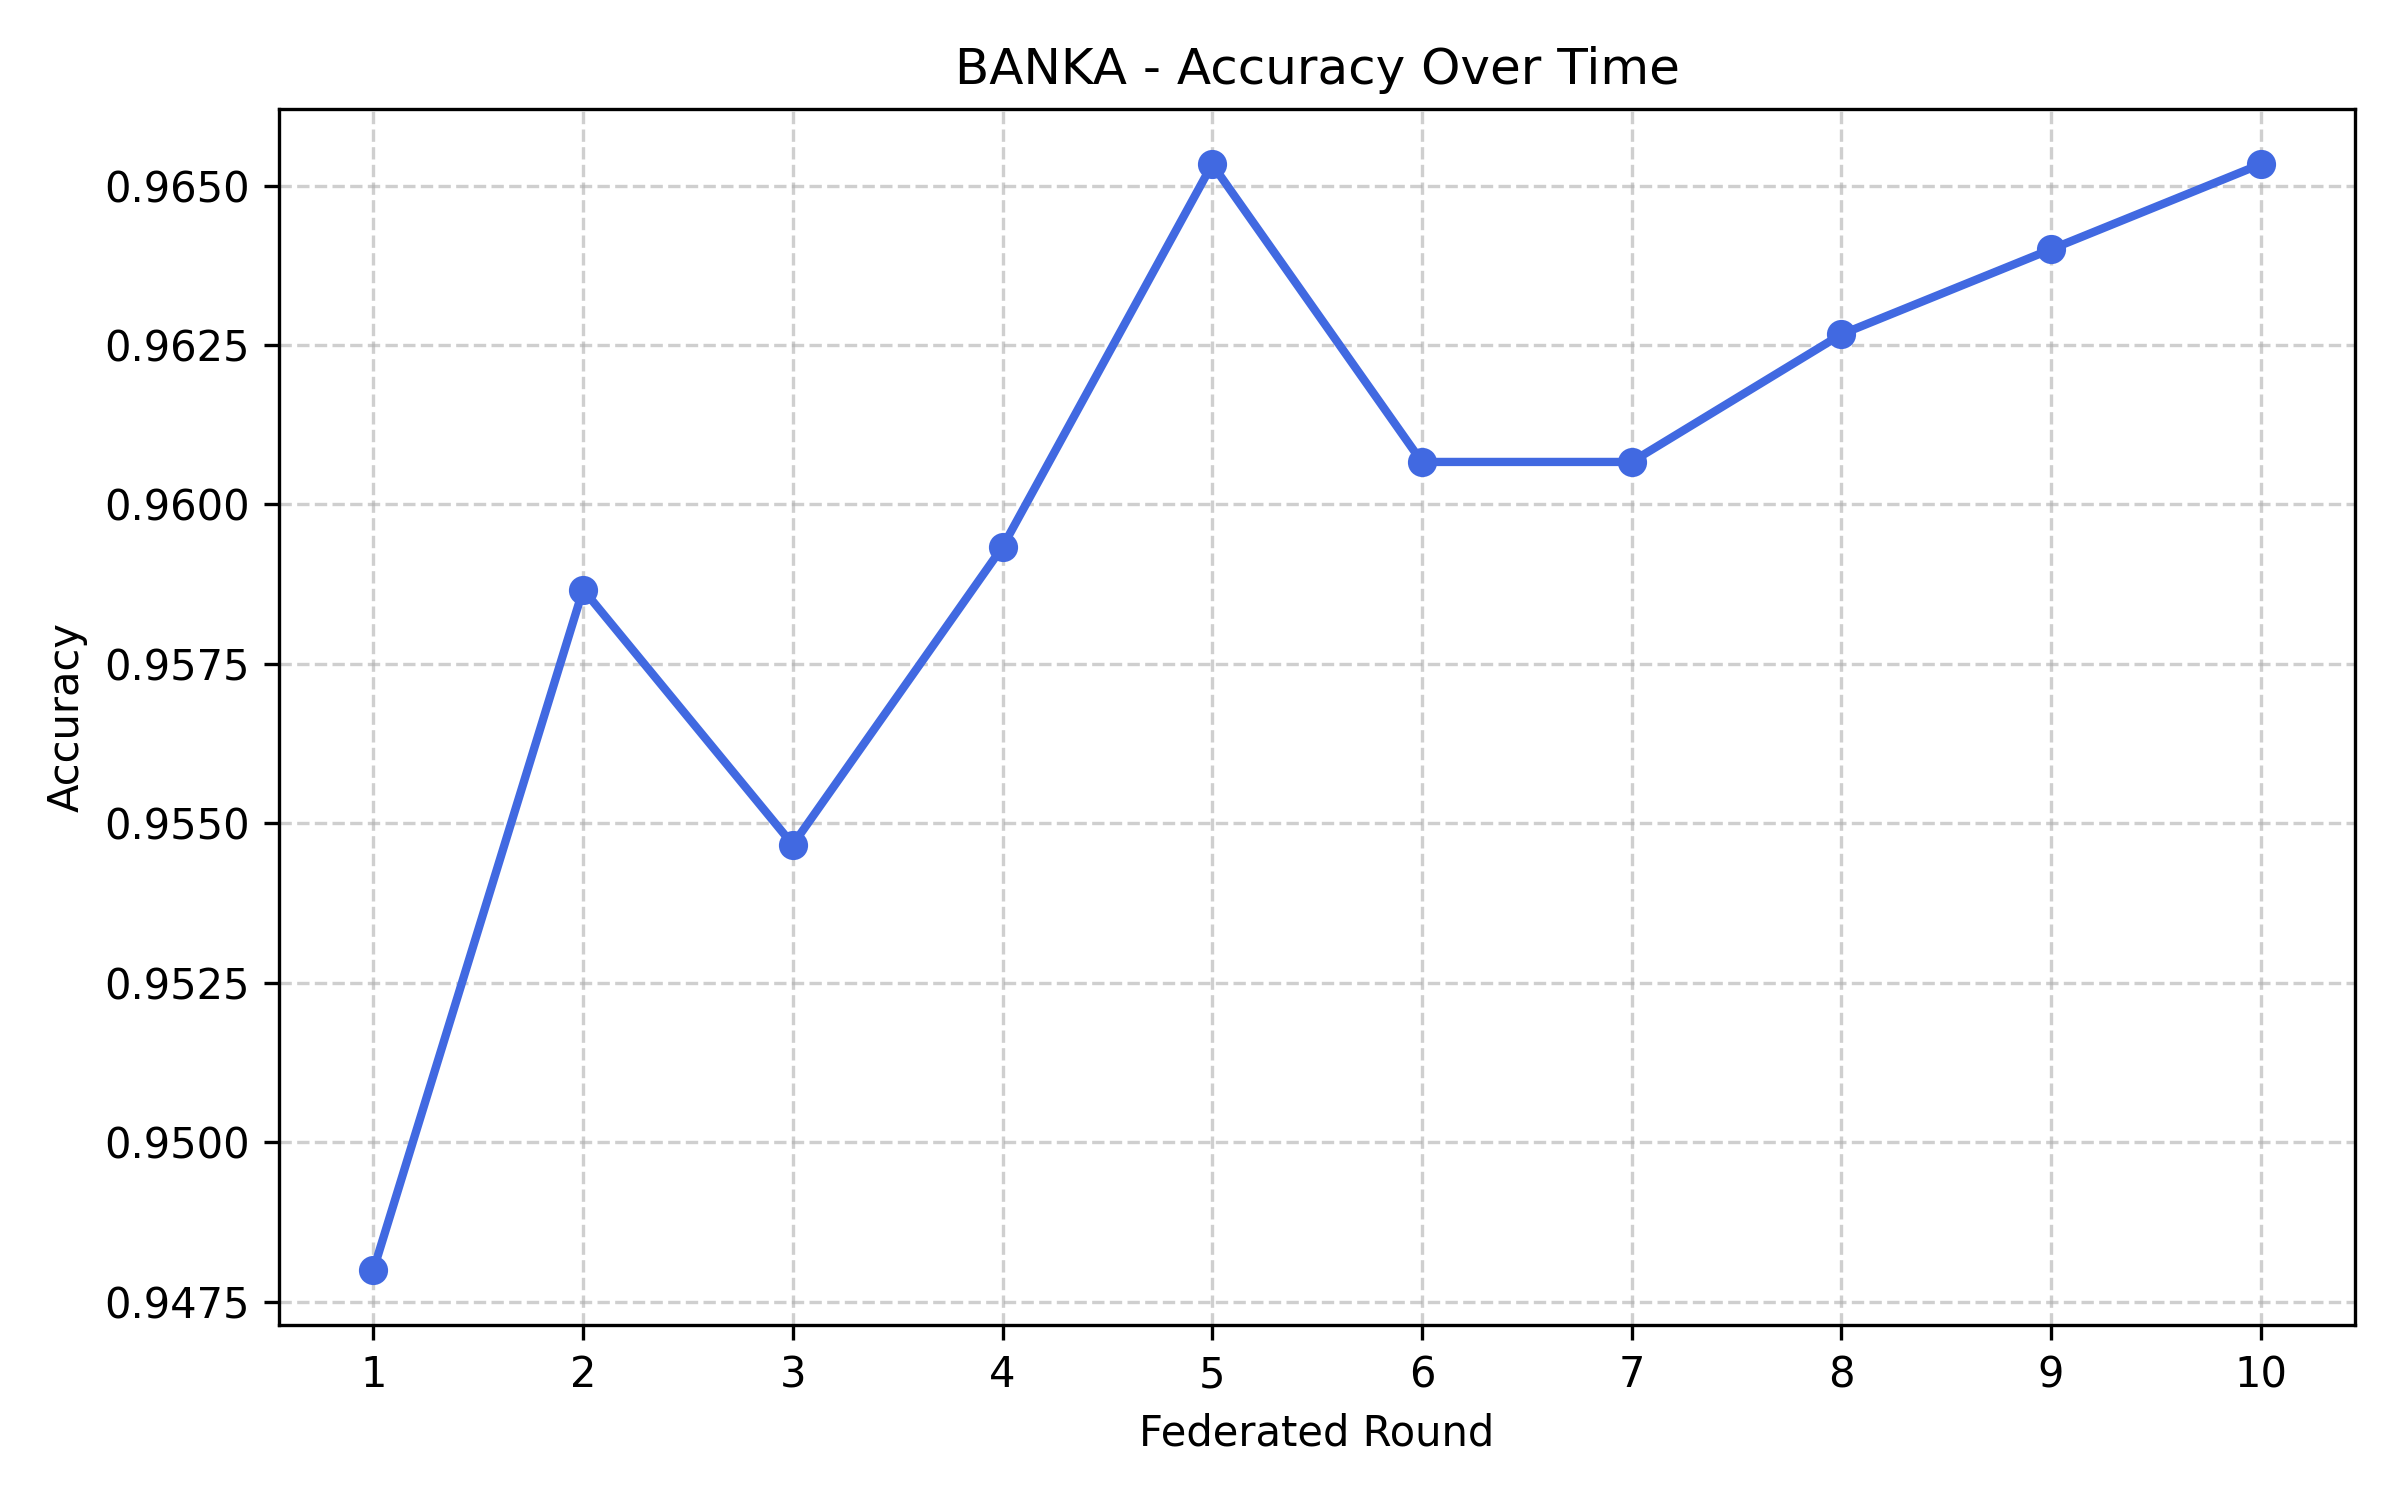
\includegraphics[width=\linewidth]{Figures/banka_progression_accuracy.png}

\vspace{0.1cm}
{\small (a) BANKA Accuracy vs Federated Aggregation Rounds}\end{minipage}
\hfill
\begin{minipage}{0.48\textwidth}
\centering
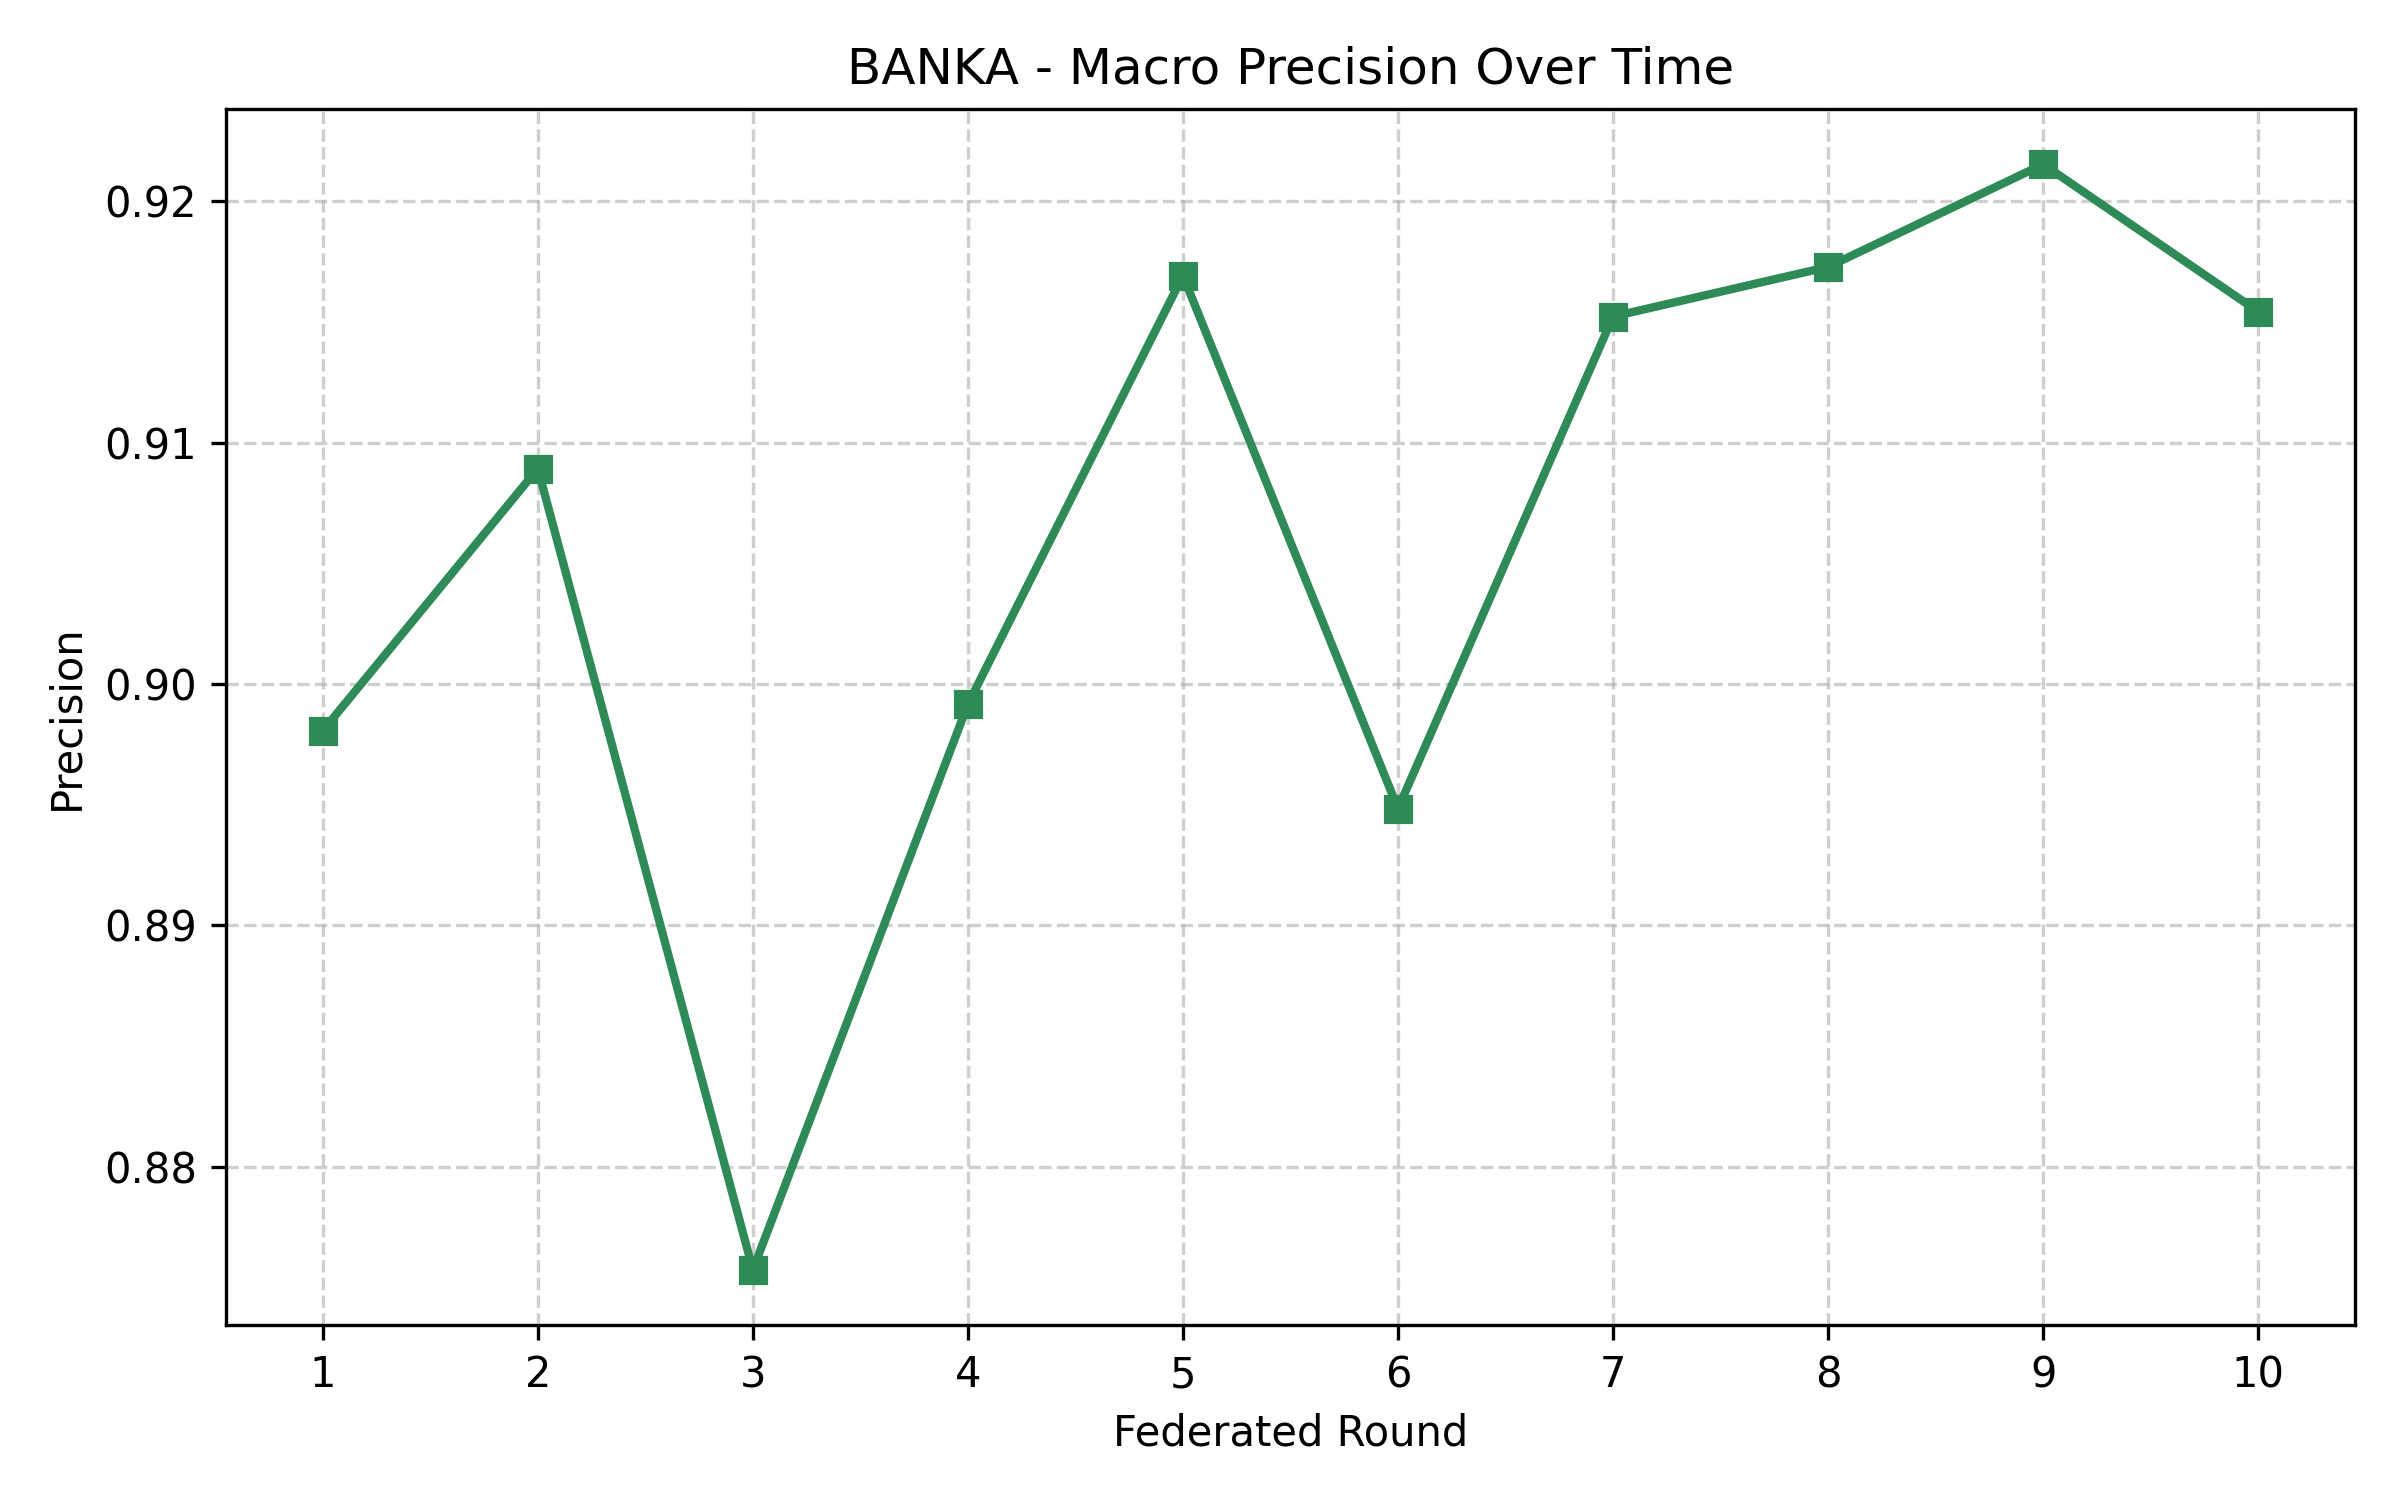
\includegraphics[width=\linewidth]{Figures/banka_progression_precision.png}

\vspace{0.1cm}
{\small (b) BANKA Precision vs Federated Aggregation Rounds}\end{minipage}
\vspace{0.4cm}

% Bottom Row
\begin{minipage}{0.48\textwidth}
\centering
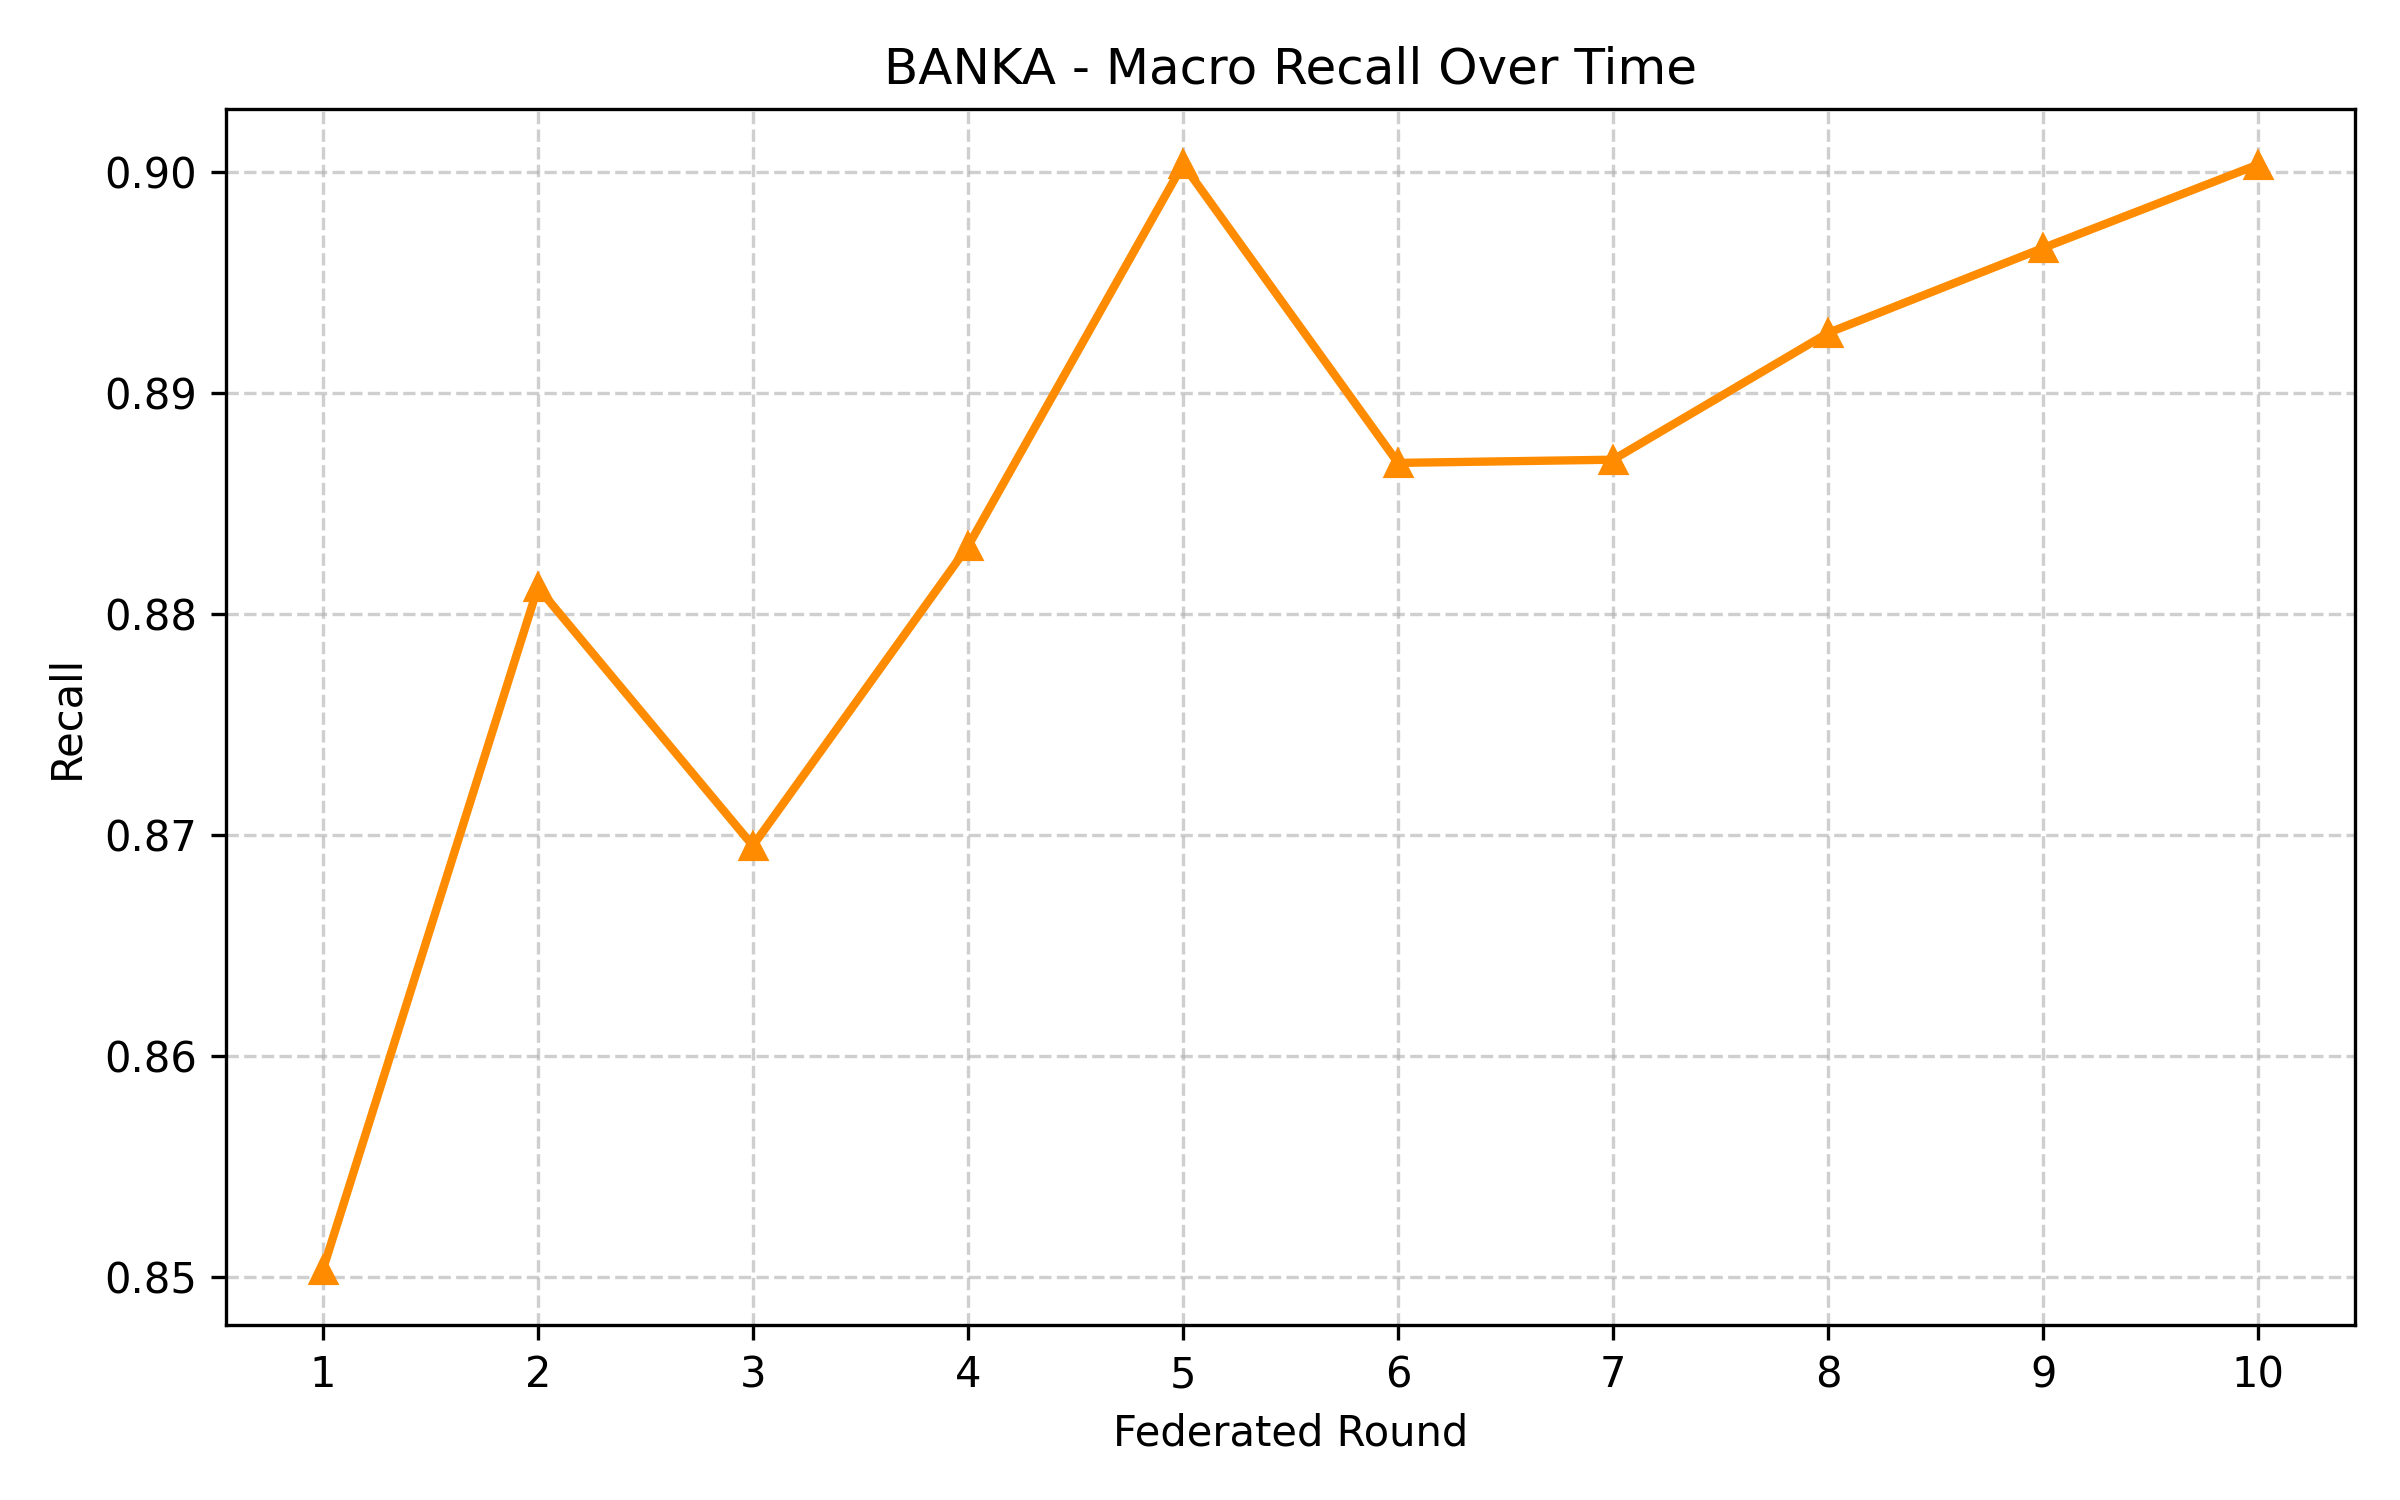
\includegraphics[width=\linewidth]{Figures/banka_progression_recall.png}

\vspace{0.1cm}
{\small (c) BANKA Recall vs Federated Aggregation Rounds}
\end{minipage}

\caption{BANKA Federated Accuracy, Precision, and Recall Progression Across Federated Aggregation Rounds}
\label{fig:banka_progression}
\end{figure}

The BANKA institutional client showed a steady increase in classification performance from round to round of federated aggregation as shown in Figure~\ref{fig:banka_progression}. The Accuracy, Precision and Recall values showed a general improvement with the going on of federated training, though minor changes were noted as it started. The accuracy rose steadily from 94.8\% to 96.5\%, and the Precision and Recall rose from 89.8\% to 91.5\% and 85.0\% to 90.0\%, respectively. The performance metrics showed less variance and more stability after the fifth aggregation round, suggesting successful convergence during the federated learning process. The observed evolution confirms the capability of distributed parameter aggregation to improve the generalization of the model and to ensure the same analytical performance in different institutional training context, without sharing any data at a central point.


%--------------------------------------------------------
\subsection{BANKB Federated Convergence}
%--------------------------------------------------------

\begin{figure}[H]
\centering

% Top Row
\begin{minipage}{0.48\textwidth}
\centering
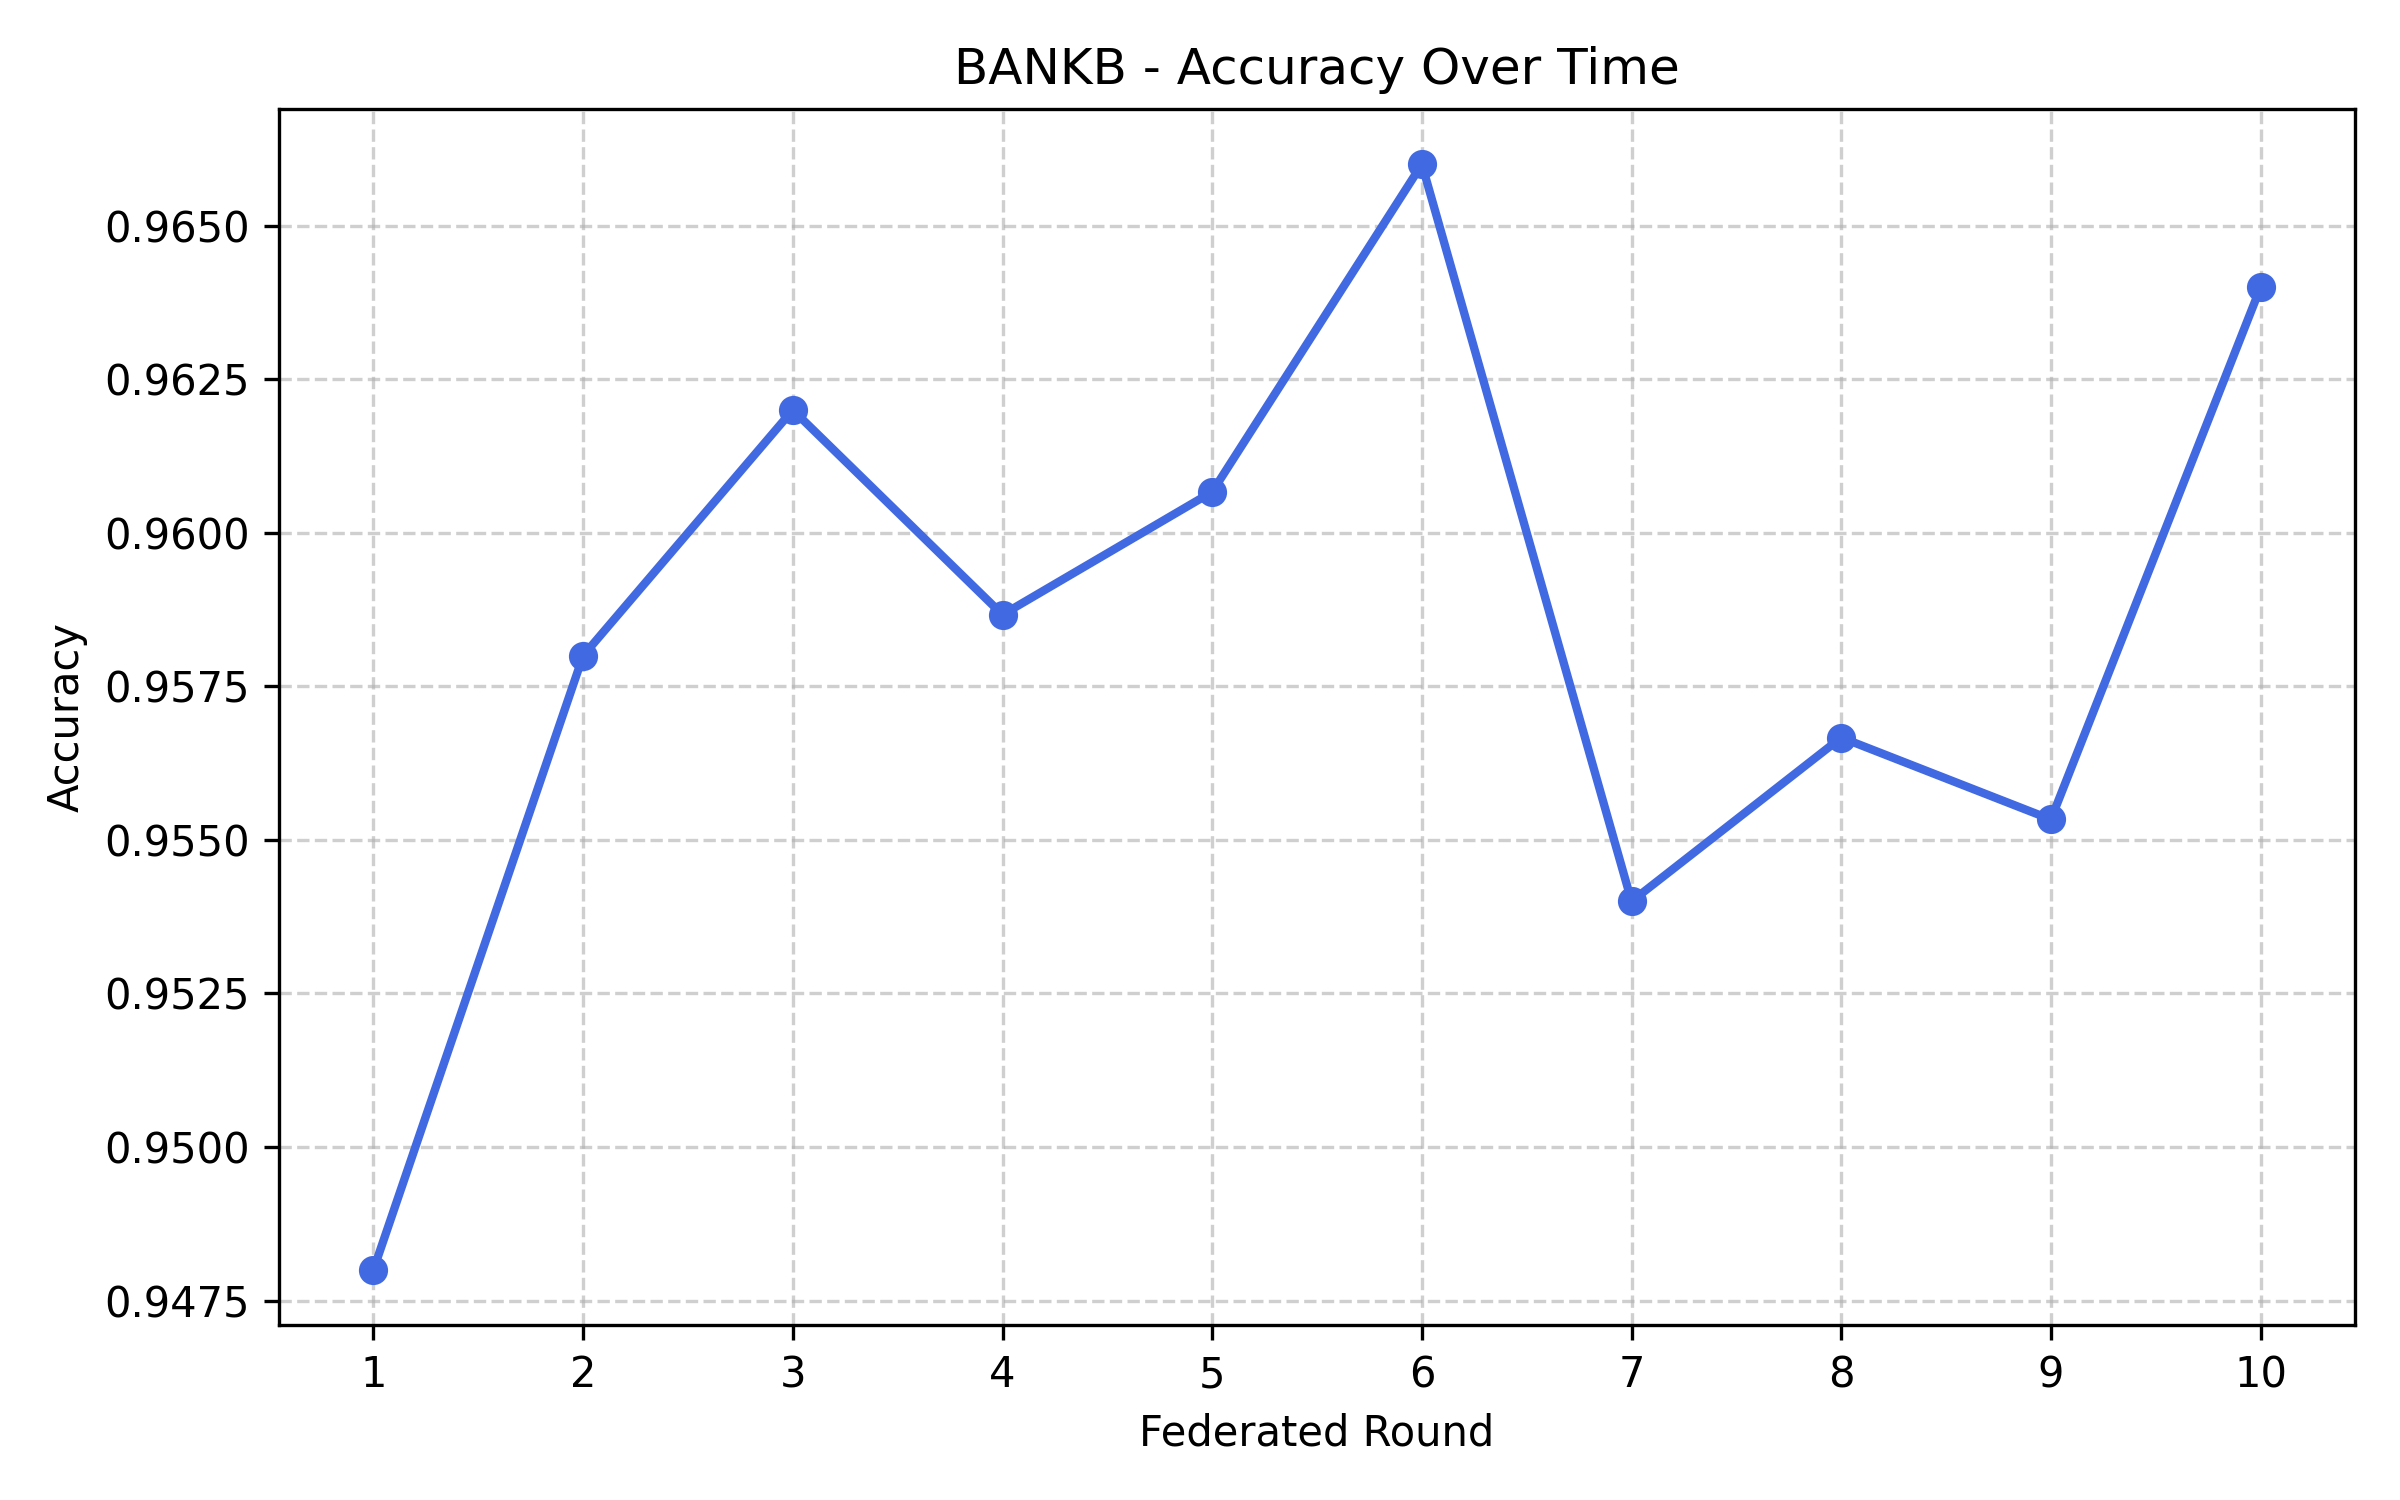
\includegraphics[width=\linewidth]{Figures/bankb_progression_accuracy.png}

\vspace{0.1cm}
{\small (a) BANKB Accuracy vs Federated Aggregation Rounds}
\end{minipage}
\hfill
\begin{minipage}{0.48\textwidth}
\centering
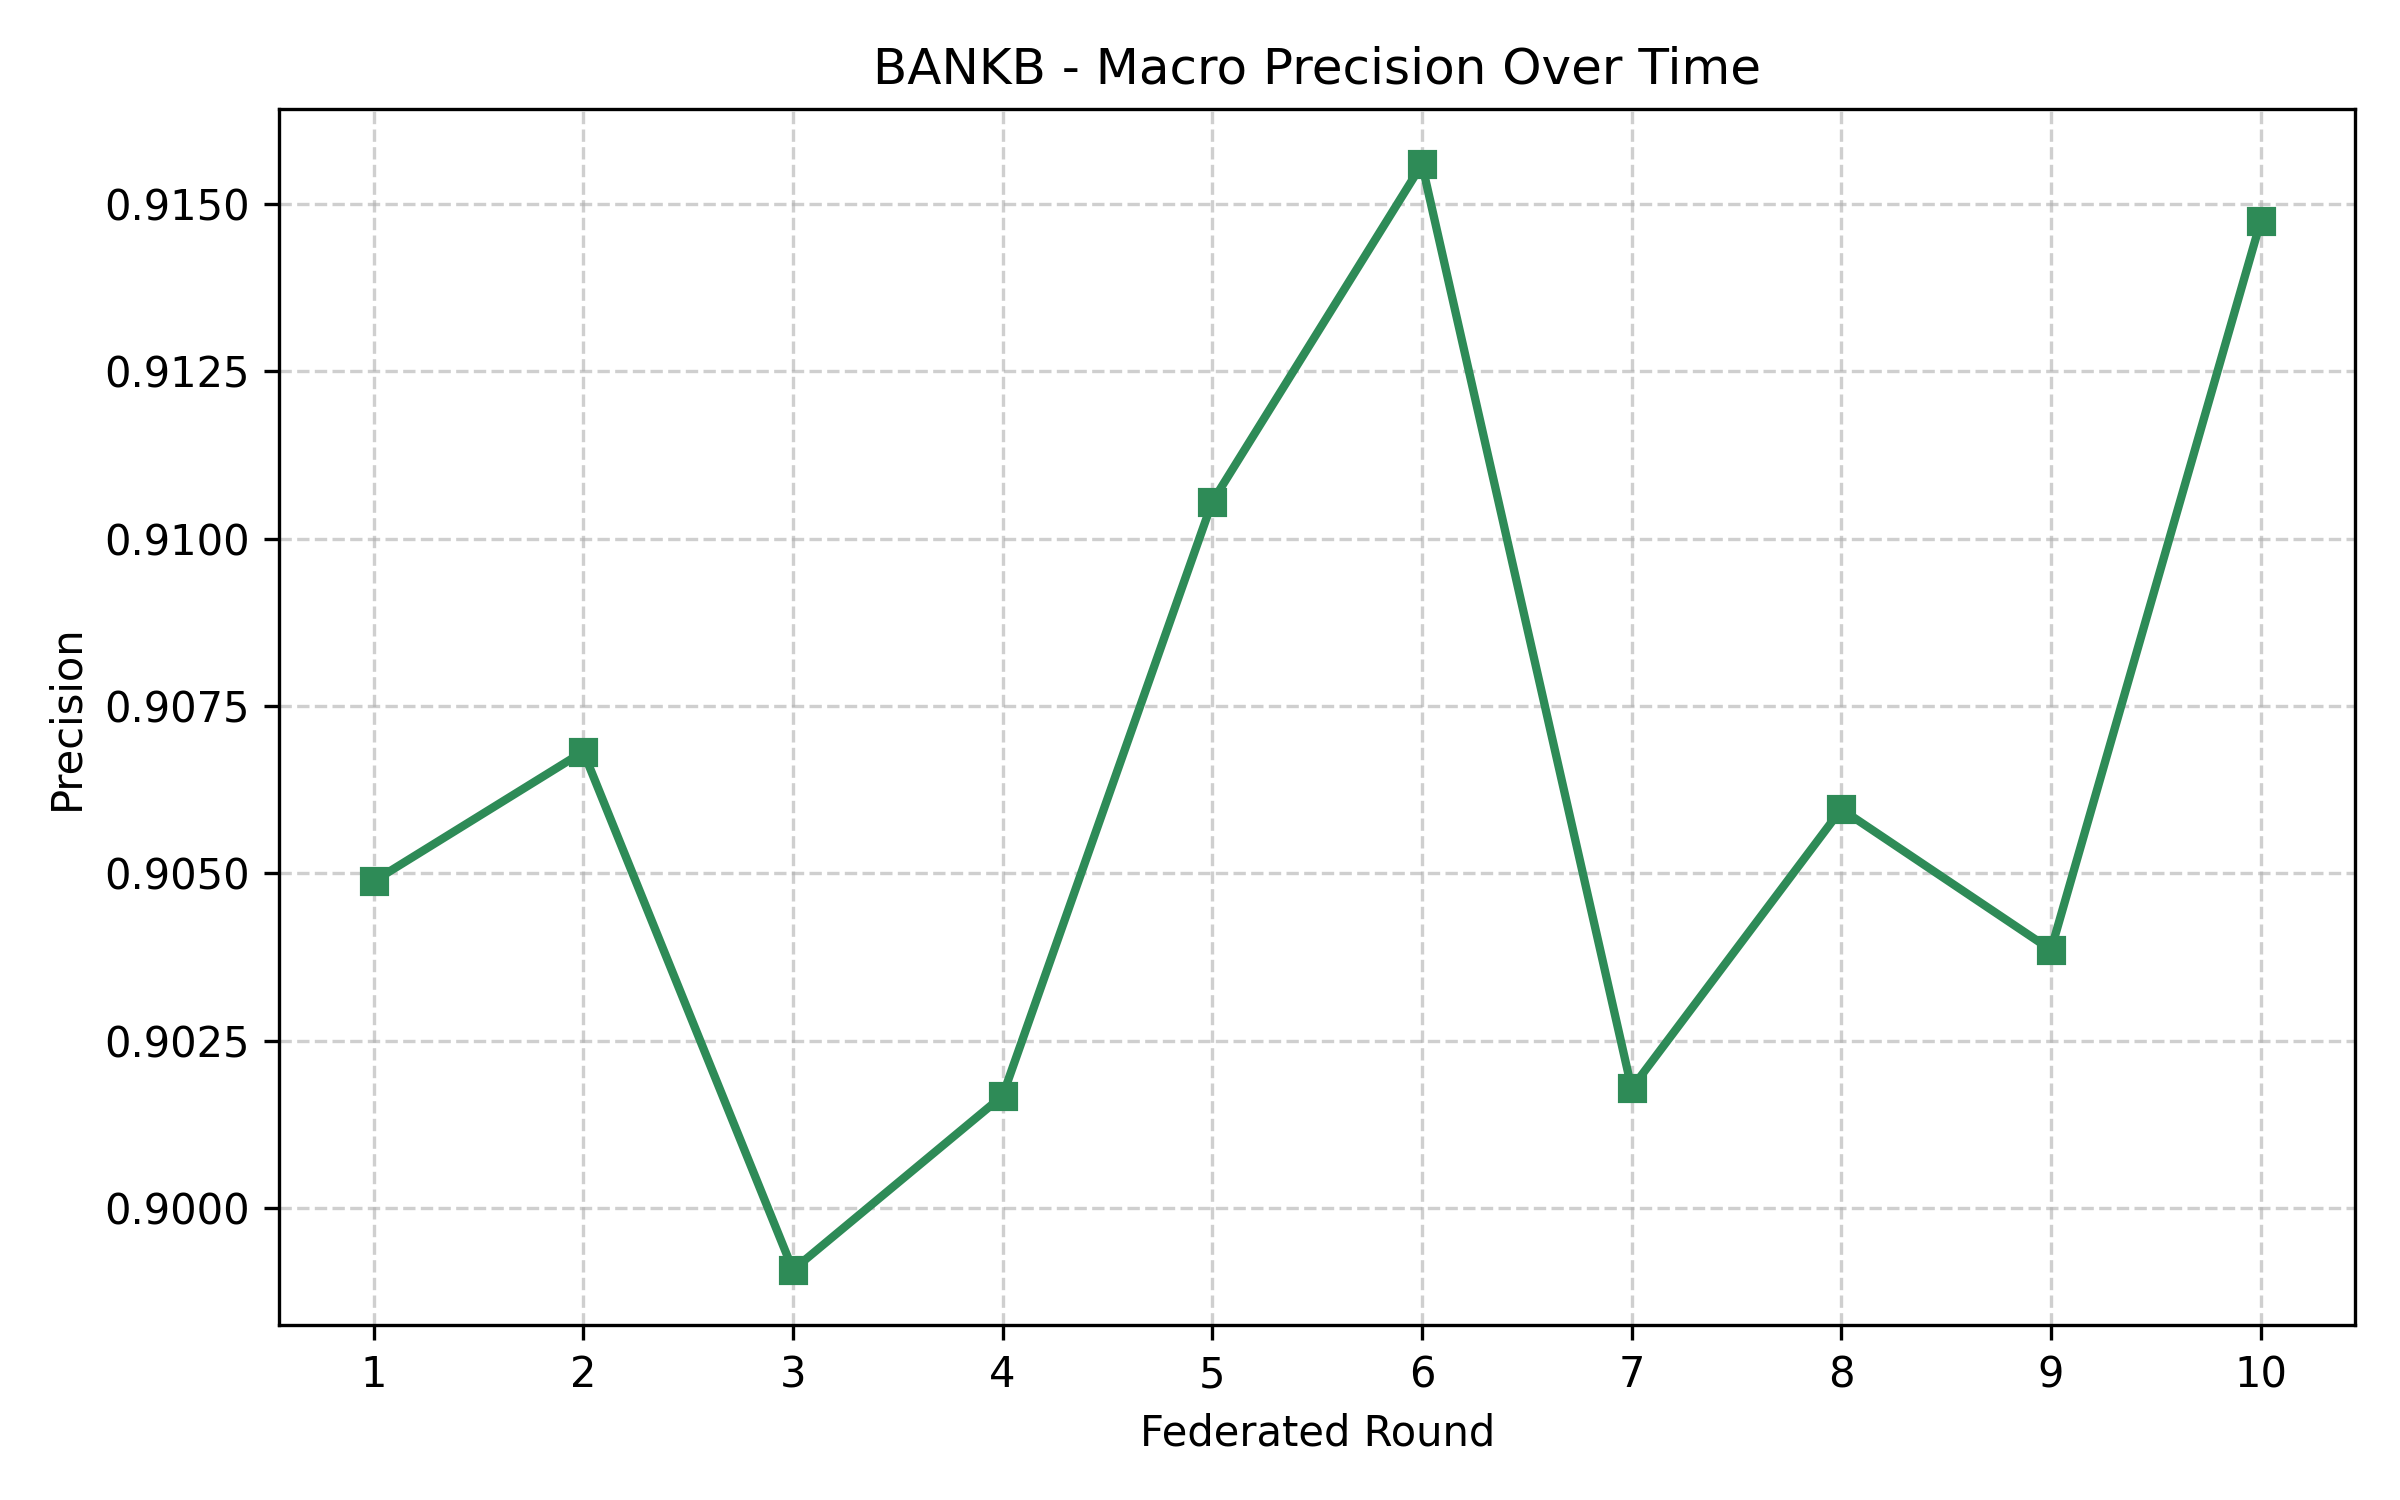
\includegraphics[width=\linewidth]{Figures/bankb_progression_precision.png}

\vspace{0.1cm}
{\small (b) BANKB Precision vs Federated Aggregation Rounds}
\end{minipage}

\vspace{0.4cm}

% Bottom Row
\begin{center}
\begin{minipage}{0.48\textwidth}
\centering
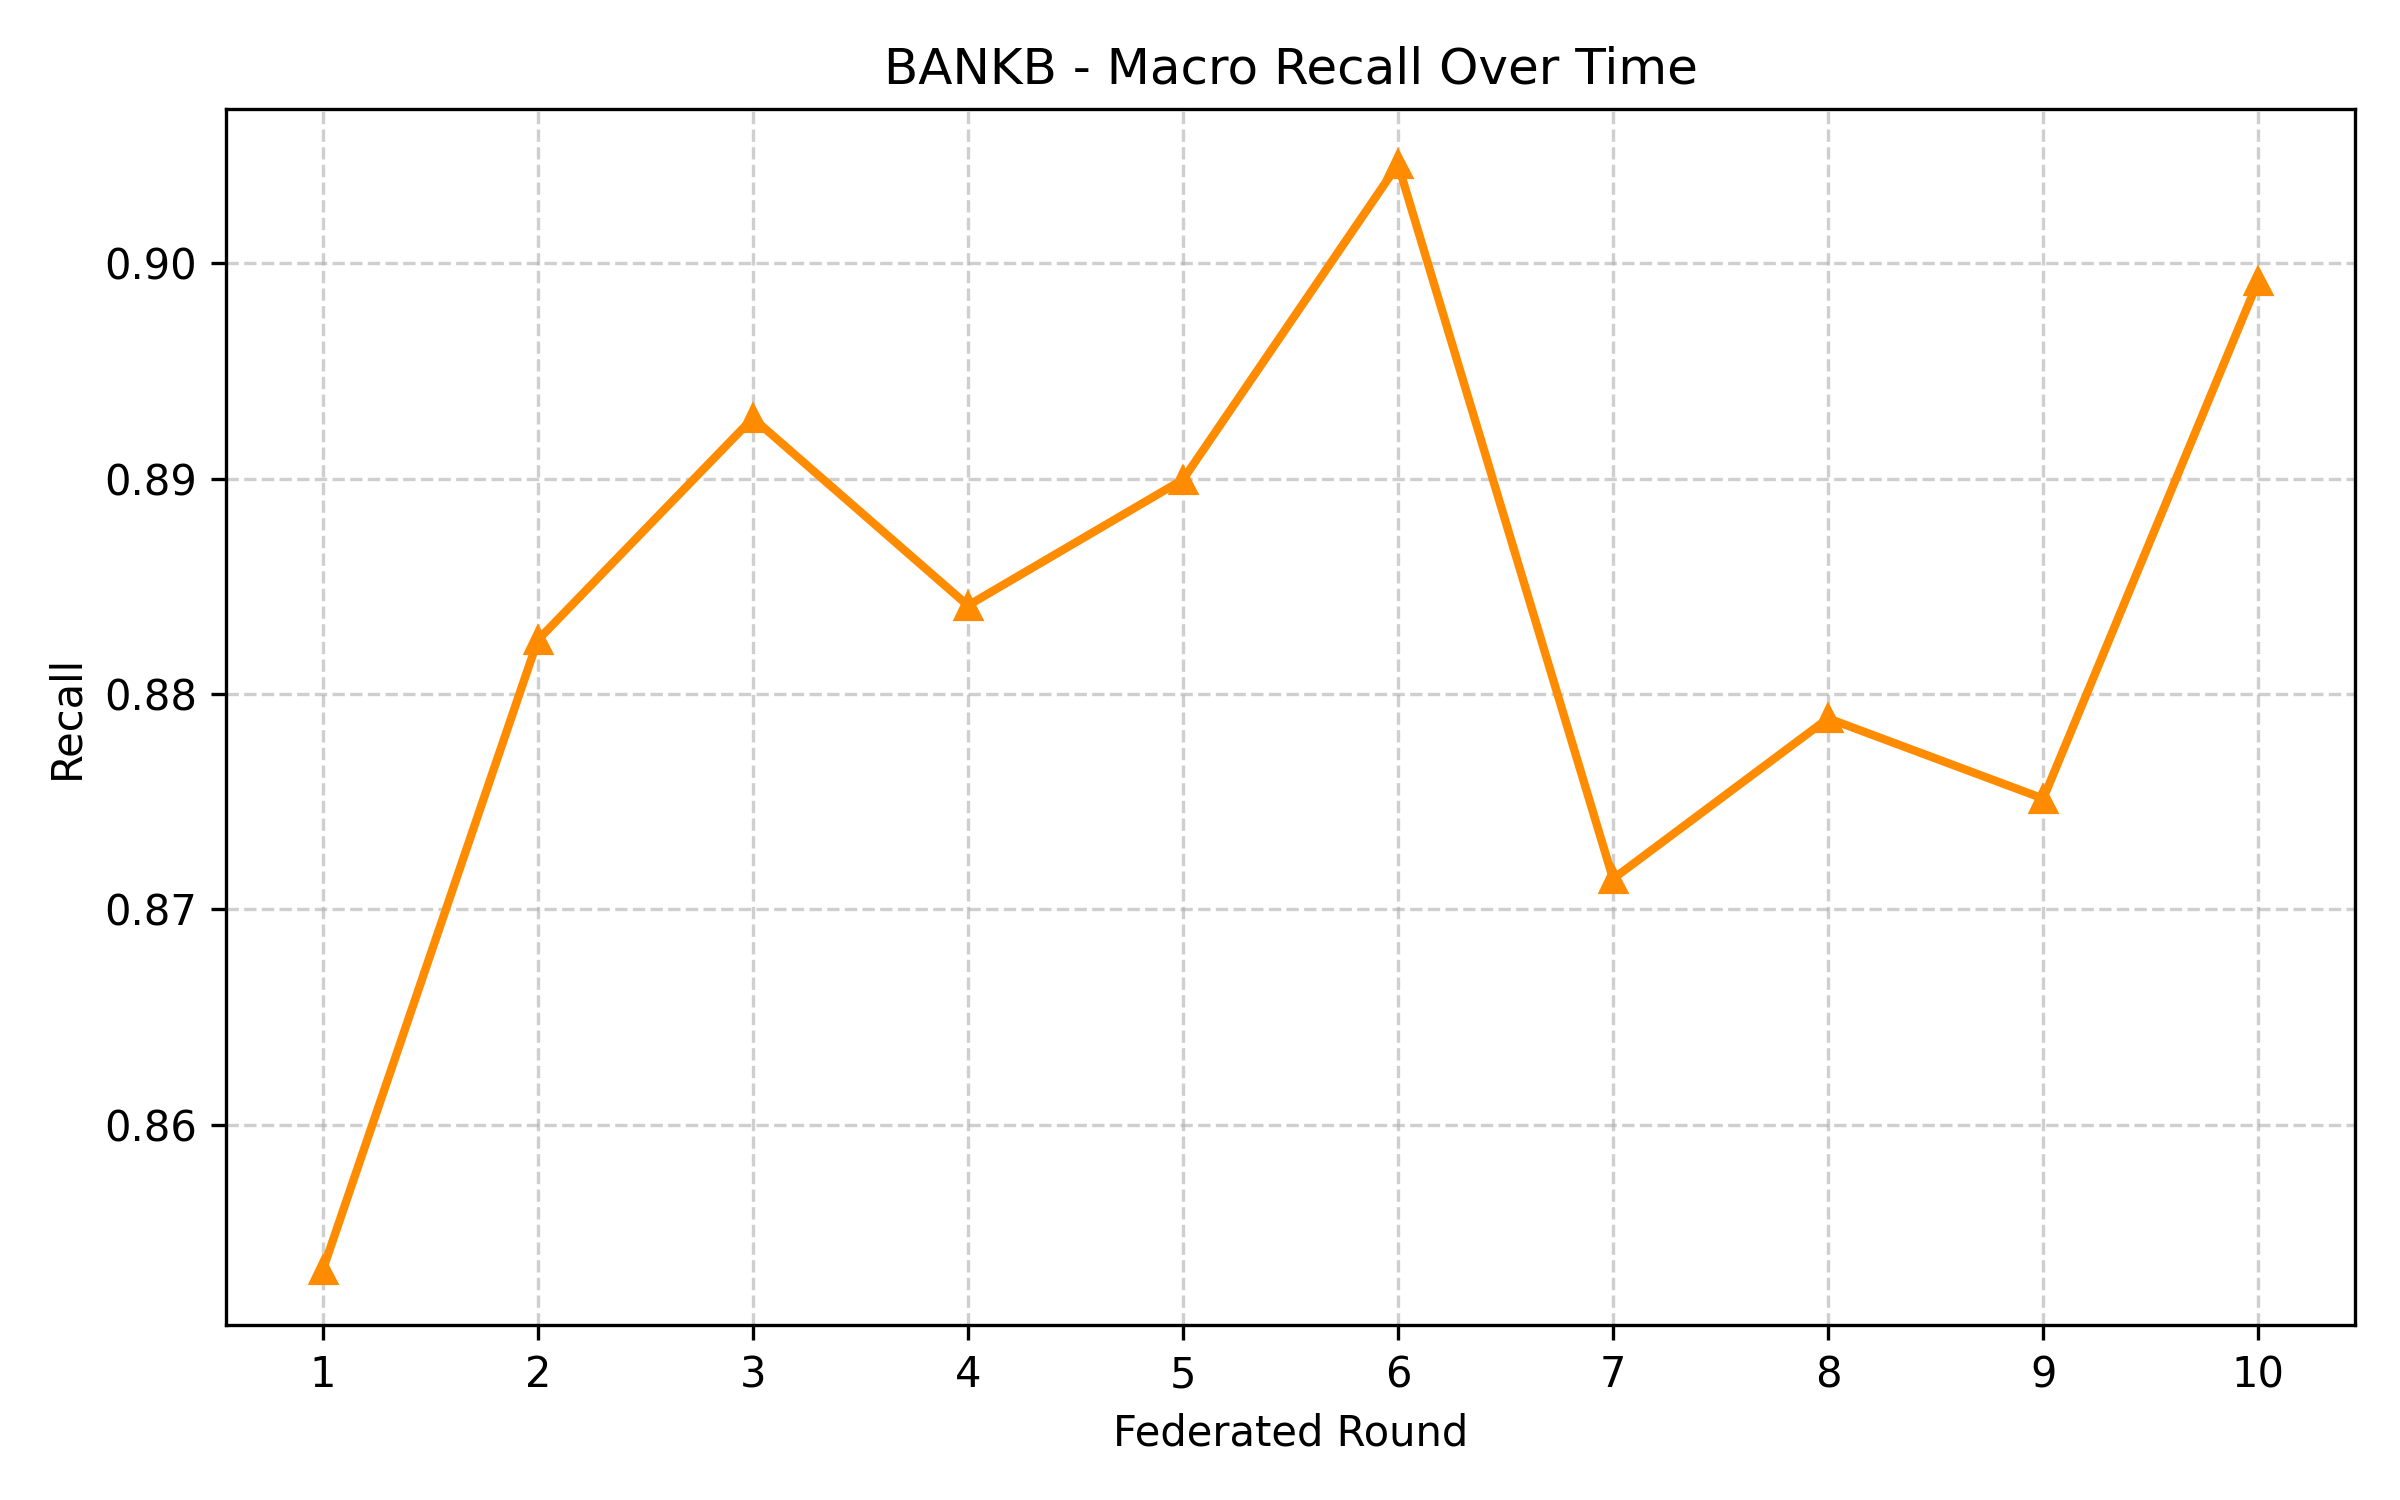
\includegraphics[width=\linewidth]{Figures/bankb_progression_recall.png}

\vspace{0.1cm}
{\small (c) BANKB Recall vs Federated Aggregation Rounds}
\end{minipage}
\end{center}

\caption{BANKB Federated Accuracy, Precision, and Recall Progression Across Federated Aggregation Rounds}
\label{fig:bankb_progression}
\end{figure}

he progressive improvement in classification performance of the BANKB institutional client can be seen in the successive rounds of federated aggregation (as shown in Figure~\ref{fig:bankb_progression}). Although there were some fluctuations in intermediate communication rounds, there was an overall increase in Accuracy, Precision, and Recall. The accuracy rose from ~94.8\% to 96.4\%, while Precision and Recall were improved from 90.5\% to 91.5\%, 85.3\% to 89.9\%, respectively. Stable parameter synchronization and subsequent updates were demonstrated as additional federated updates were applied to recover temporary performance fluctuations seen in later rounds of the experiment.Stable parameter synchronization and further model development was evidenced by additional federated updates in subsequent rounds of the experiment, which recovered temporary performance variations observed in earlier rounds. The final aggregation rounds delivered very robust analytical results with a level of federated convergence and knowledge sharing between distributed institutional training environments that did not provide any centralised data exchange.

%--------------------------------------------------------
\subsection{BANKC Federated Convergence}
%--------------------------------------------------------
\begin{figure}[H]
\centering

% Top Row
\begin{minipage}{0.48\textwidth}
\centering
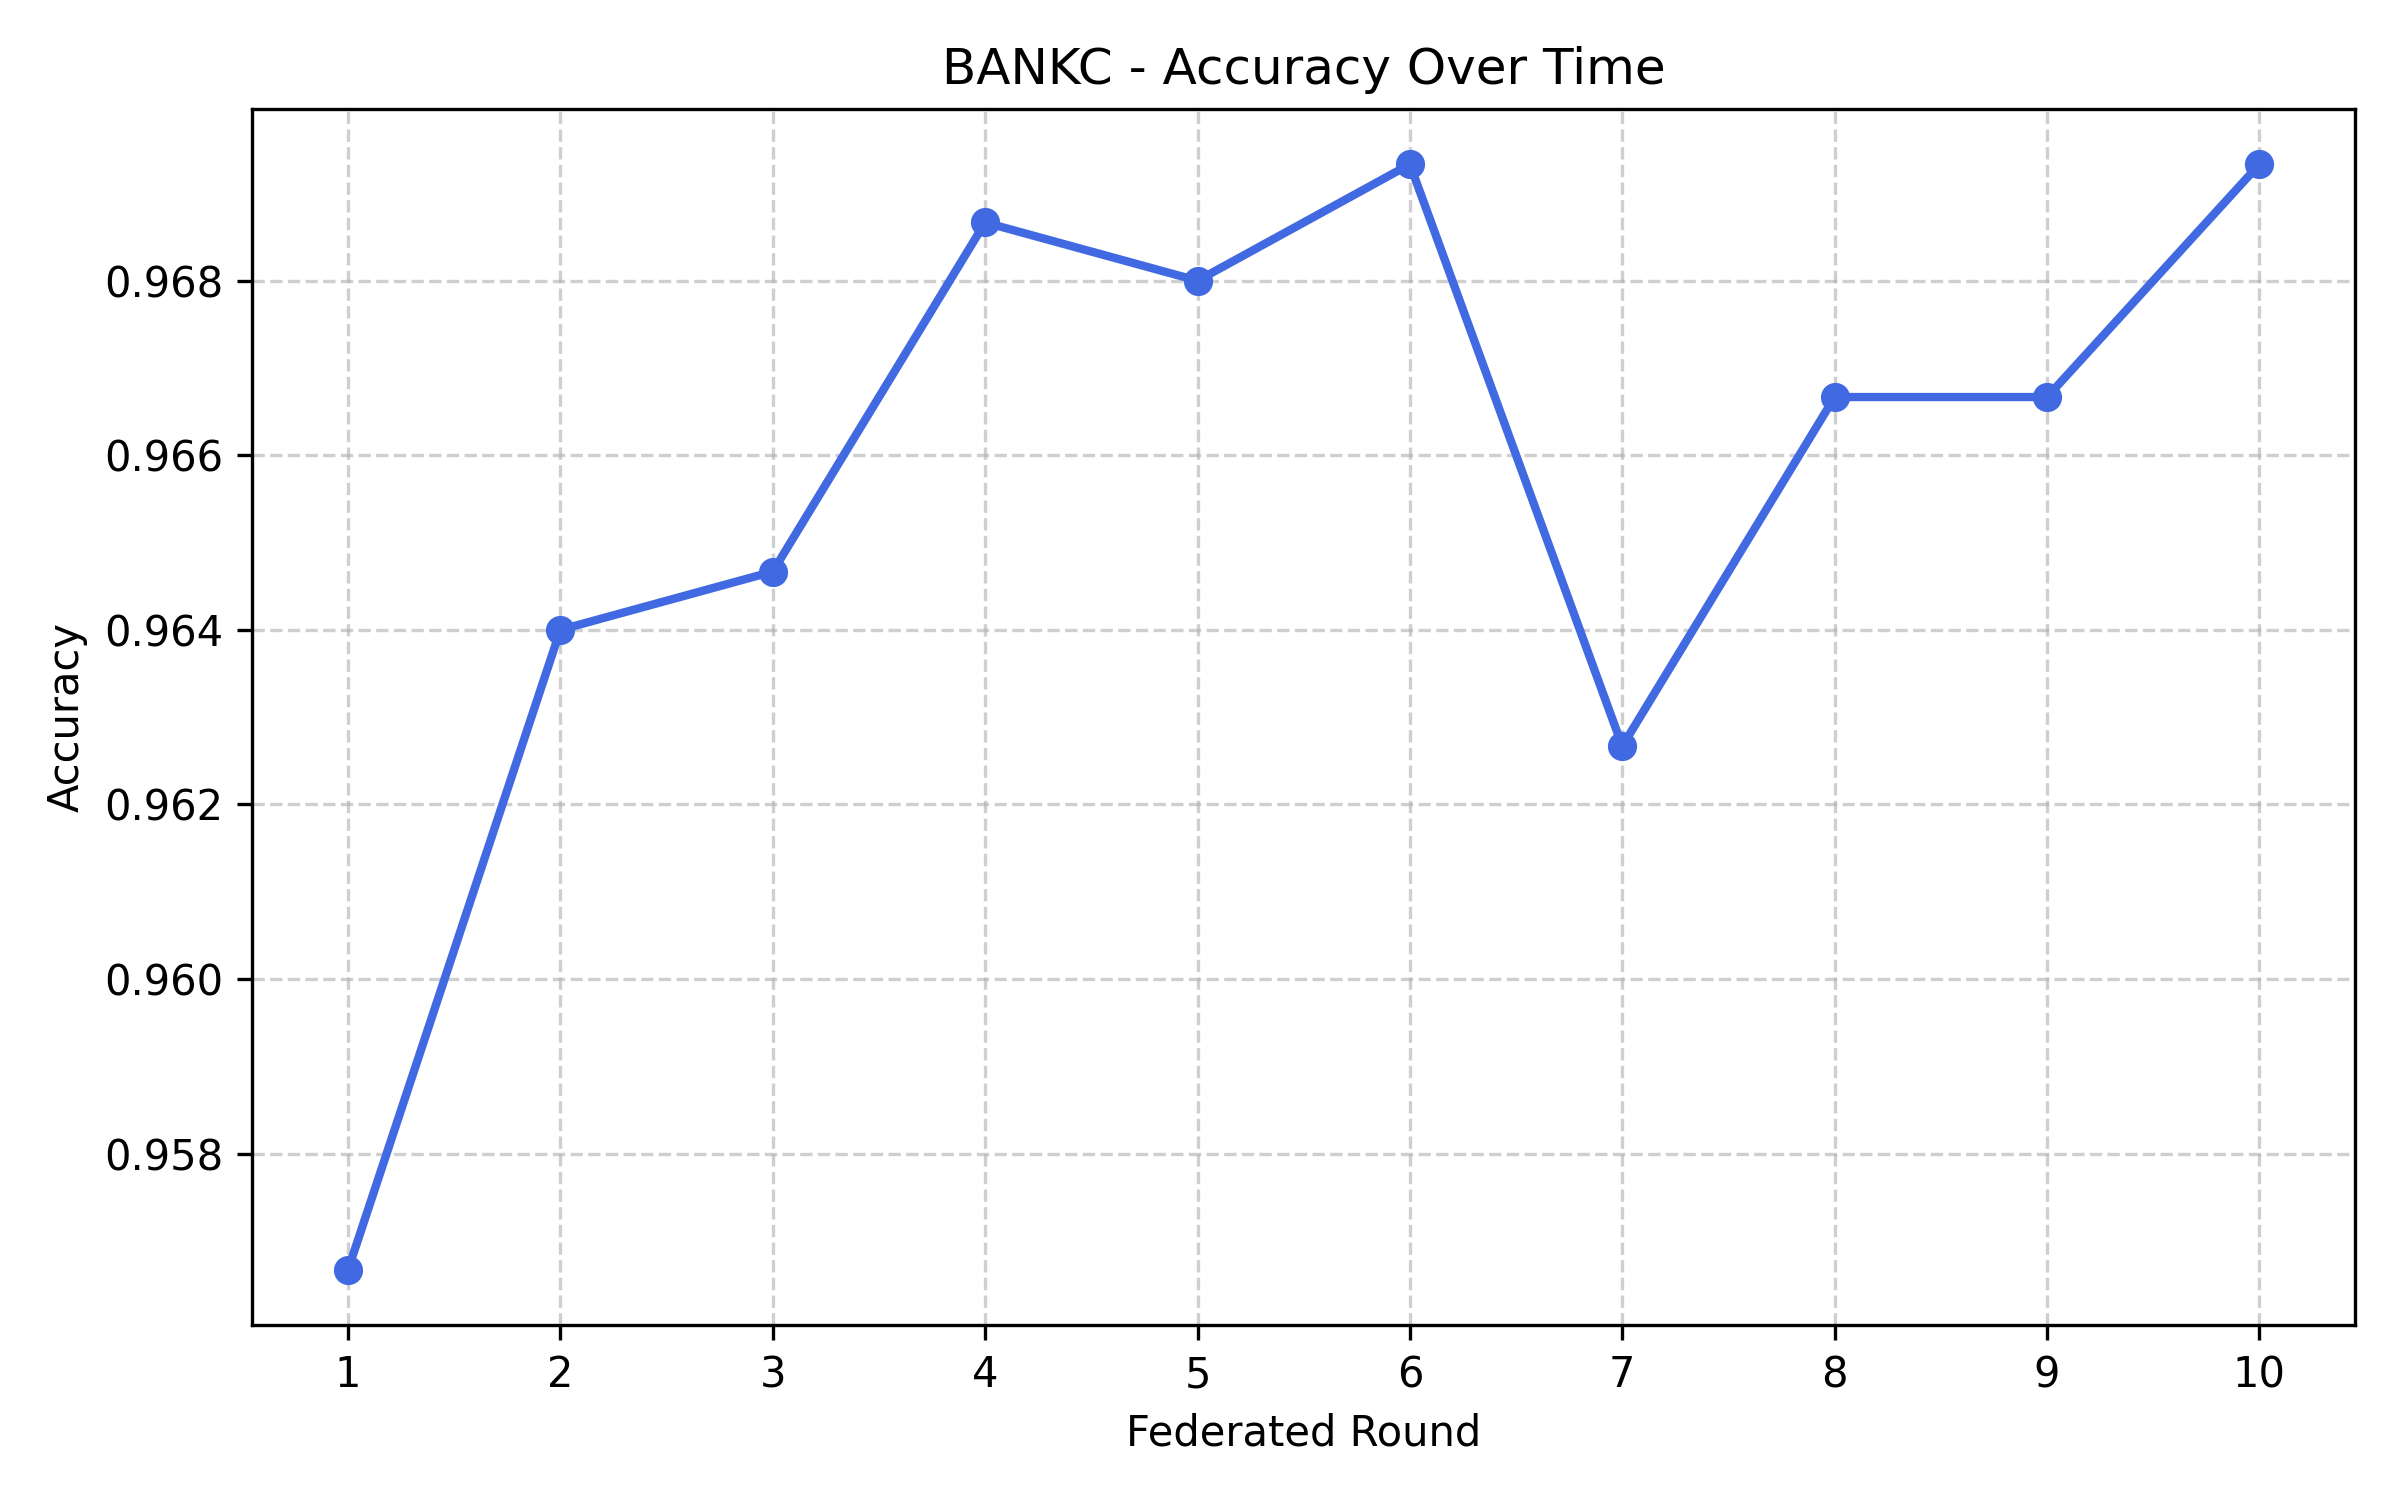
\includegraphics[width=\linewidth]{Figures/bankc_progression_accuracy.png}

\vspace{0.1cm}
{\small (a) BANKC Accuracy vs Federated Aggregation Rounds}
\end{minipage}
\hfill
\begin{minipage}{0.48\textwidth}
\centering
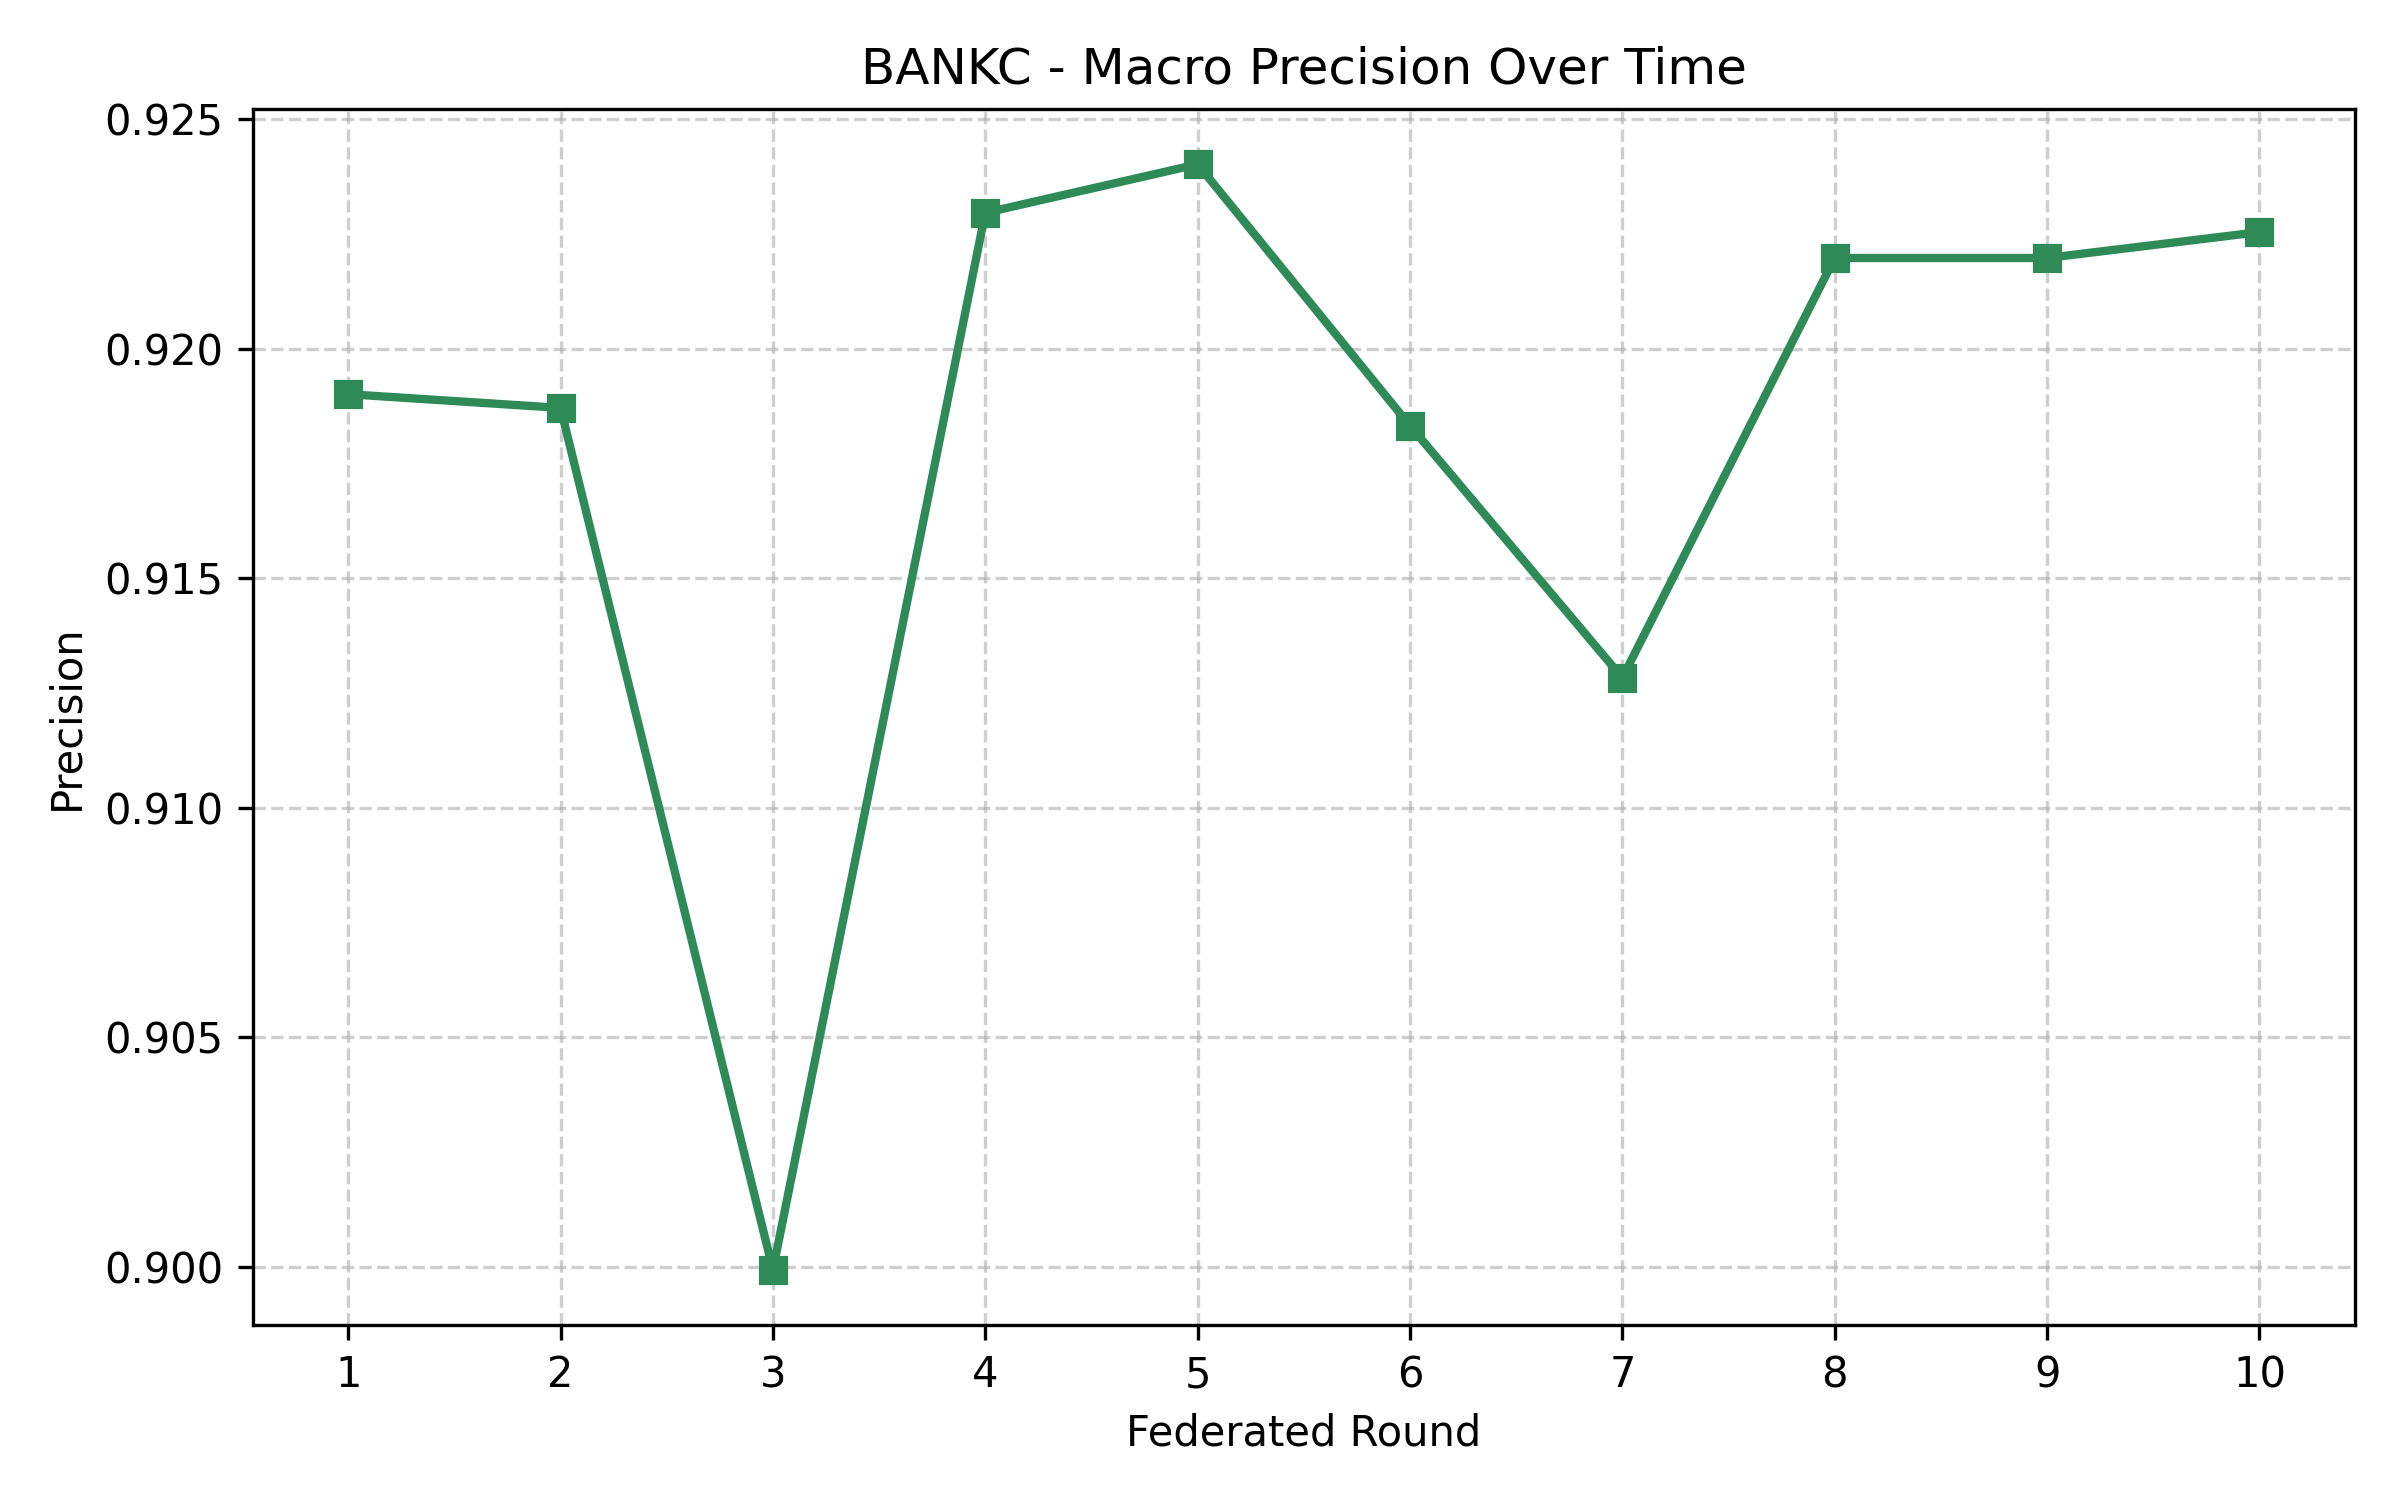
\includegraphics[width=\linewidth]{Figures/bankc_progression_precision.png}

\vspace{0.1cm}
{\small (b) BANKC Precision vs Federated Aggregation Rounds}
\end{minipage}

\vspace{0.4cm}

% Bottom Row
\begin{center}
\begin{minipage}{0.48\textwidth}
\centering
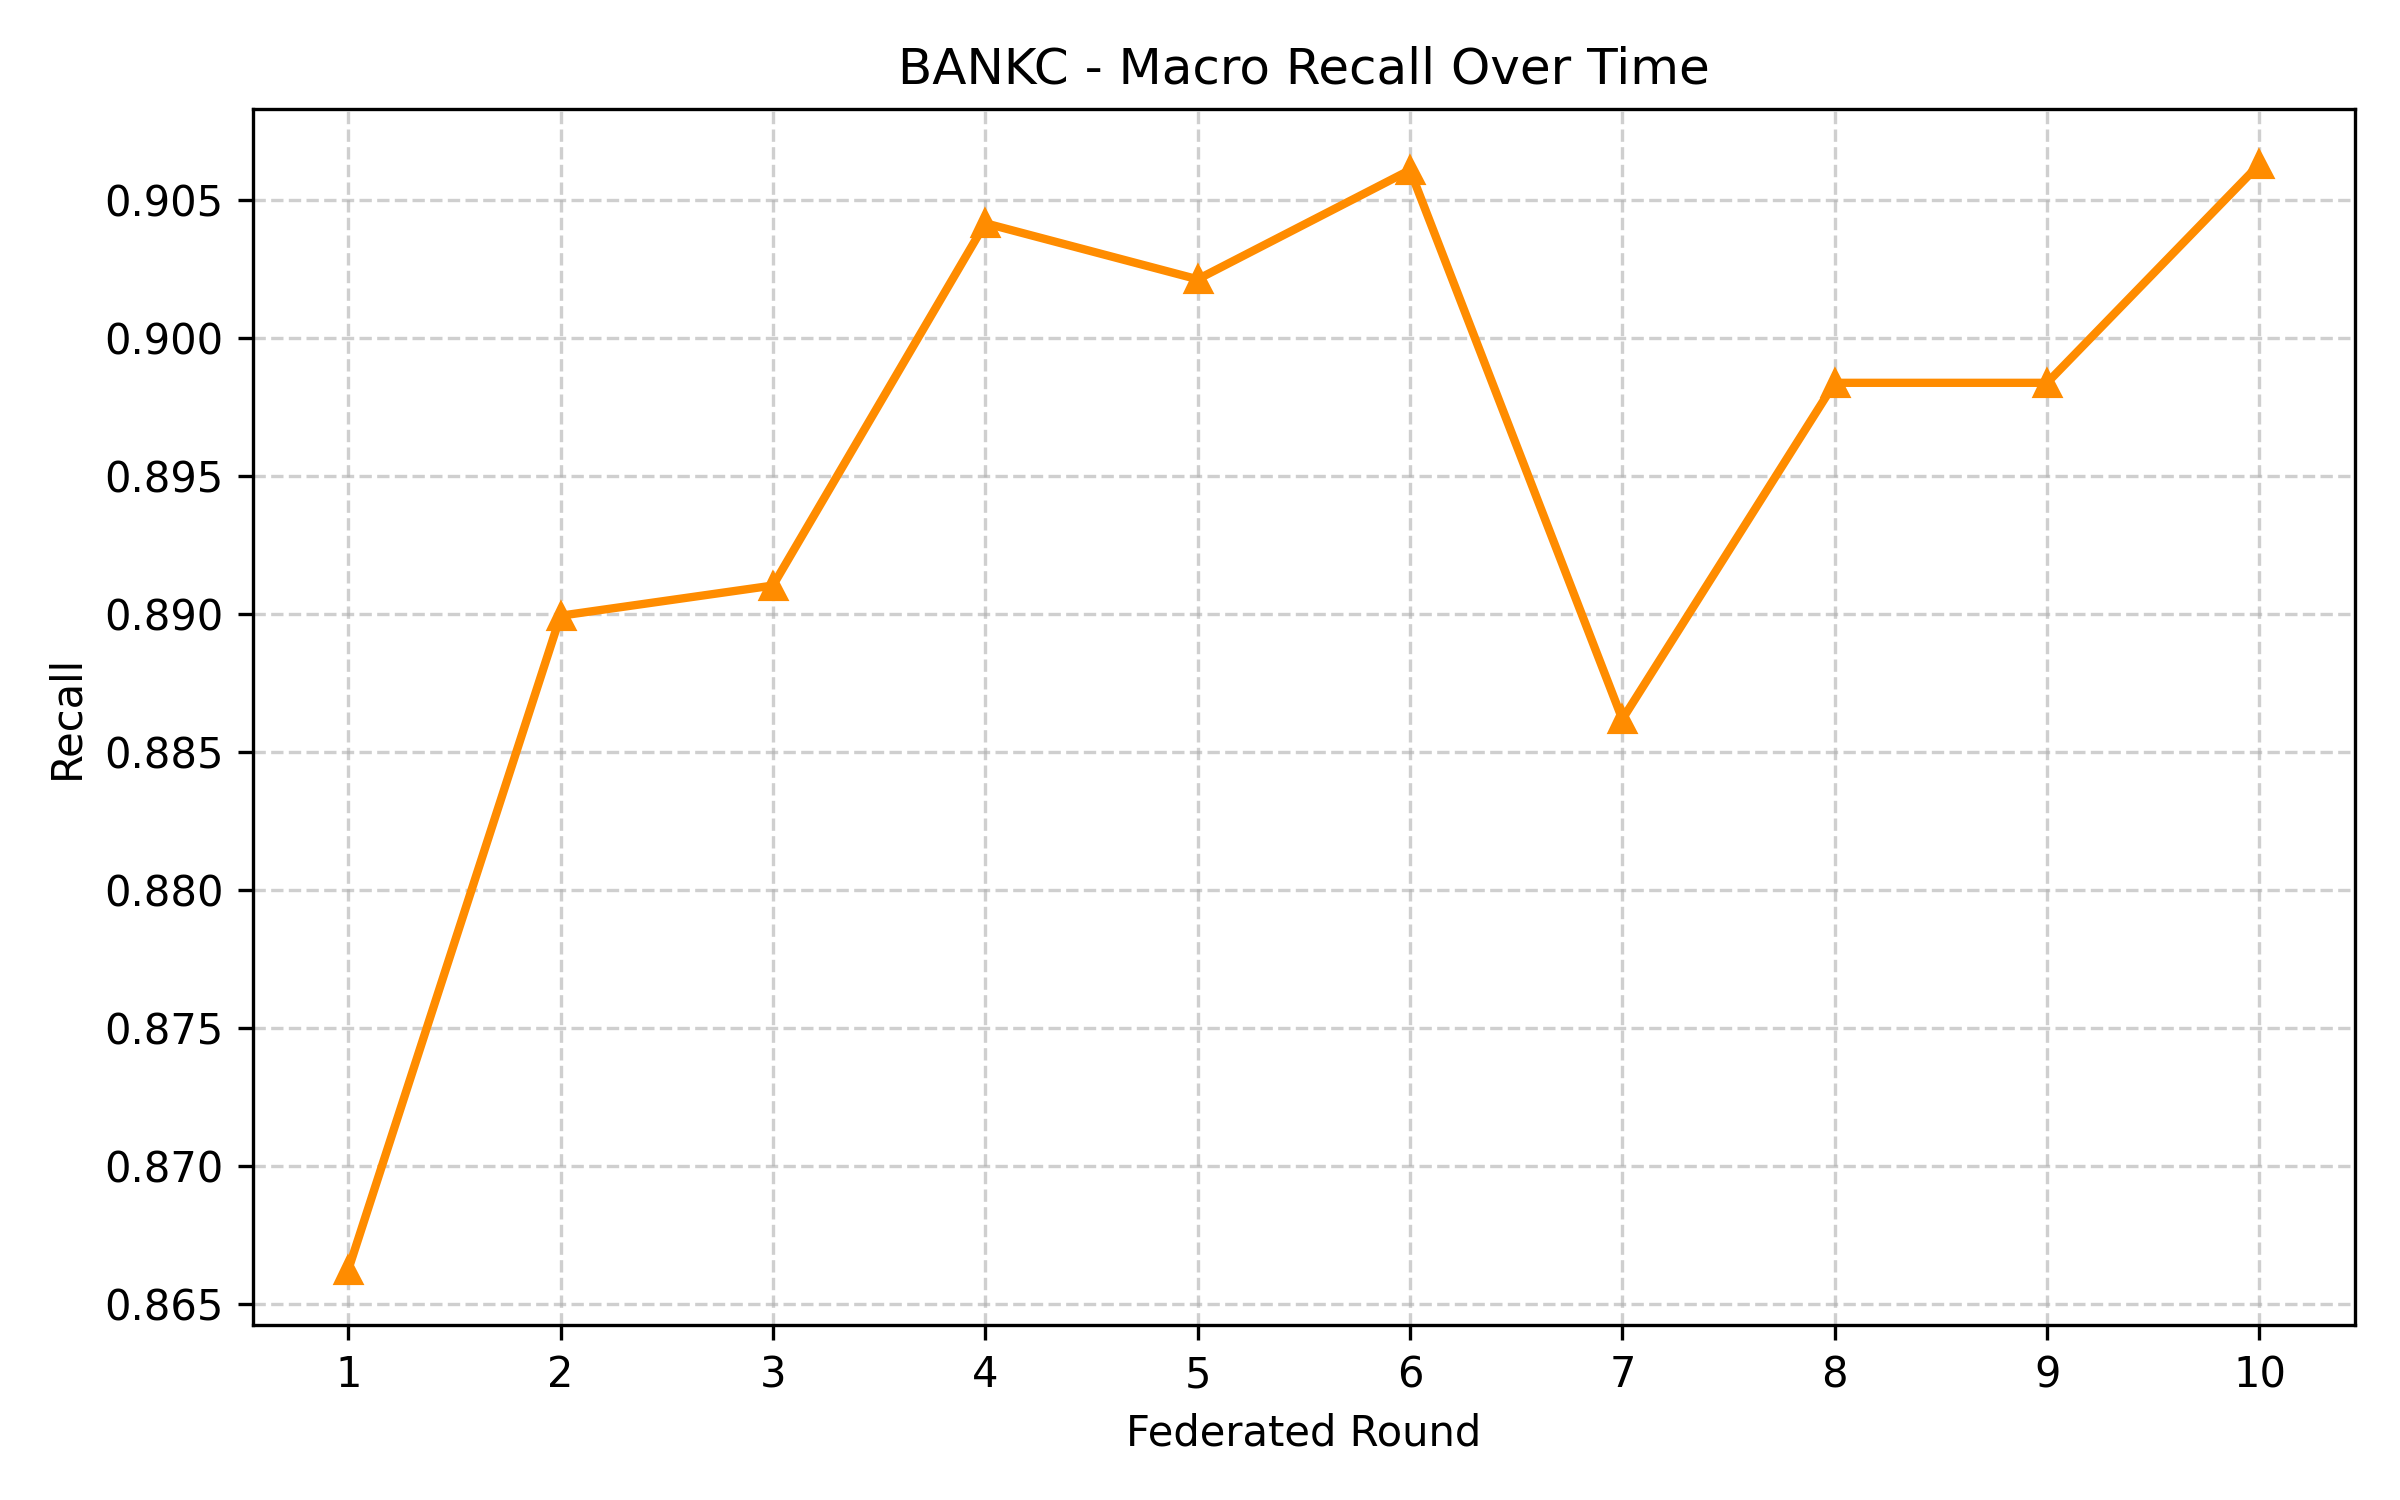
\includegraphics[width=\linewidth]{Figures/bankc_progression_recall.png}

\vspace{0.1cm}
{\small (c) BANKC Recall vs Federated Aggregation Rounds}
\end{minipage}
\end{center}

\caption{BANKC Federated Accuracy, Precision, and Recall Progression Across Federated Aggregation Rounds}
\label{fig:bankc_progression}
\end{figure}
The BANKC institutional client showed a very consistent federated convergence behaviour for successive aggregation rounds as shown in Figure~\ref{fig:bankc_progression}. The metrics of Accuracy (ACC), Precision (PRC), and Recall (RCL) all showed a gradual increase in the first few rounds of the initial communication phase, but afterwards, the data for the rest of the federated rounds were relatively stable with only slight variations. The accuracy elevates from about 95.7% to 96.9%, Precision and Recall reaches almost 92.2% and 90.6% respectively. Minimal performance fluctuations were noted at intermediate synchronization phases, although the metrics quickly stabilized and stayed in a small range, suggesting the successful distributed parameter aggregation and good model generalization. The observed convergence characteristics confirm the stable federated optimization and the framework's capability to keep the analytical performance stable in a heterogeneous institutional transaction environment while keeping the data out of the central repository.
%========================================================
\subsection[Precision--Recall and Confusion Matrix Validation]{\textbf{Precision--Recall and Confusion Matrix Validation}}
%========================================================

Precision-Recall analytical validation and confusion matrix analysis was performed to test for discrimination capabilities against fraud, minority class recognition behavior, and false positive propagation within distributed institutional settings. As fraudulent transactional activity accounted for only a small percentage of all transactional activity within institutions, Precision-Recall validation offered a more practical test than pure classification accuracy.
BANKA Precision-Recall and Confusion Matrix Validation


%--------------------------------------------------------
\subsubsection{BANKA Precision--Recall and Confusion Matrix Validation}
%--------------------------------------------------------

\begin{figure}[H]
\centering

\begin{minipage}{0.48\textwidth}
\centering
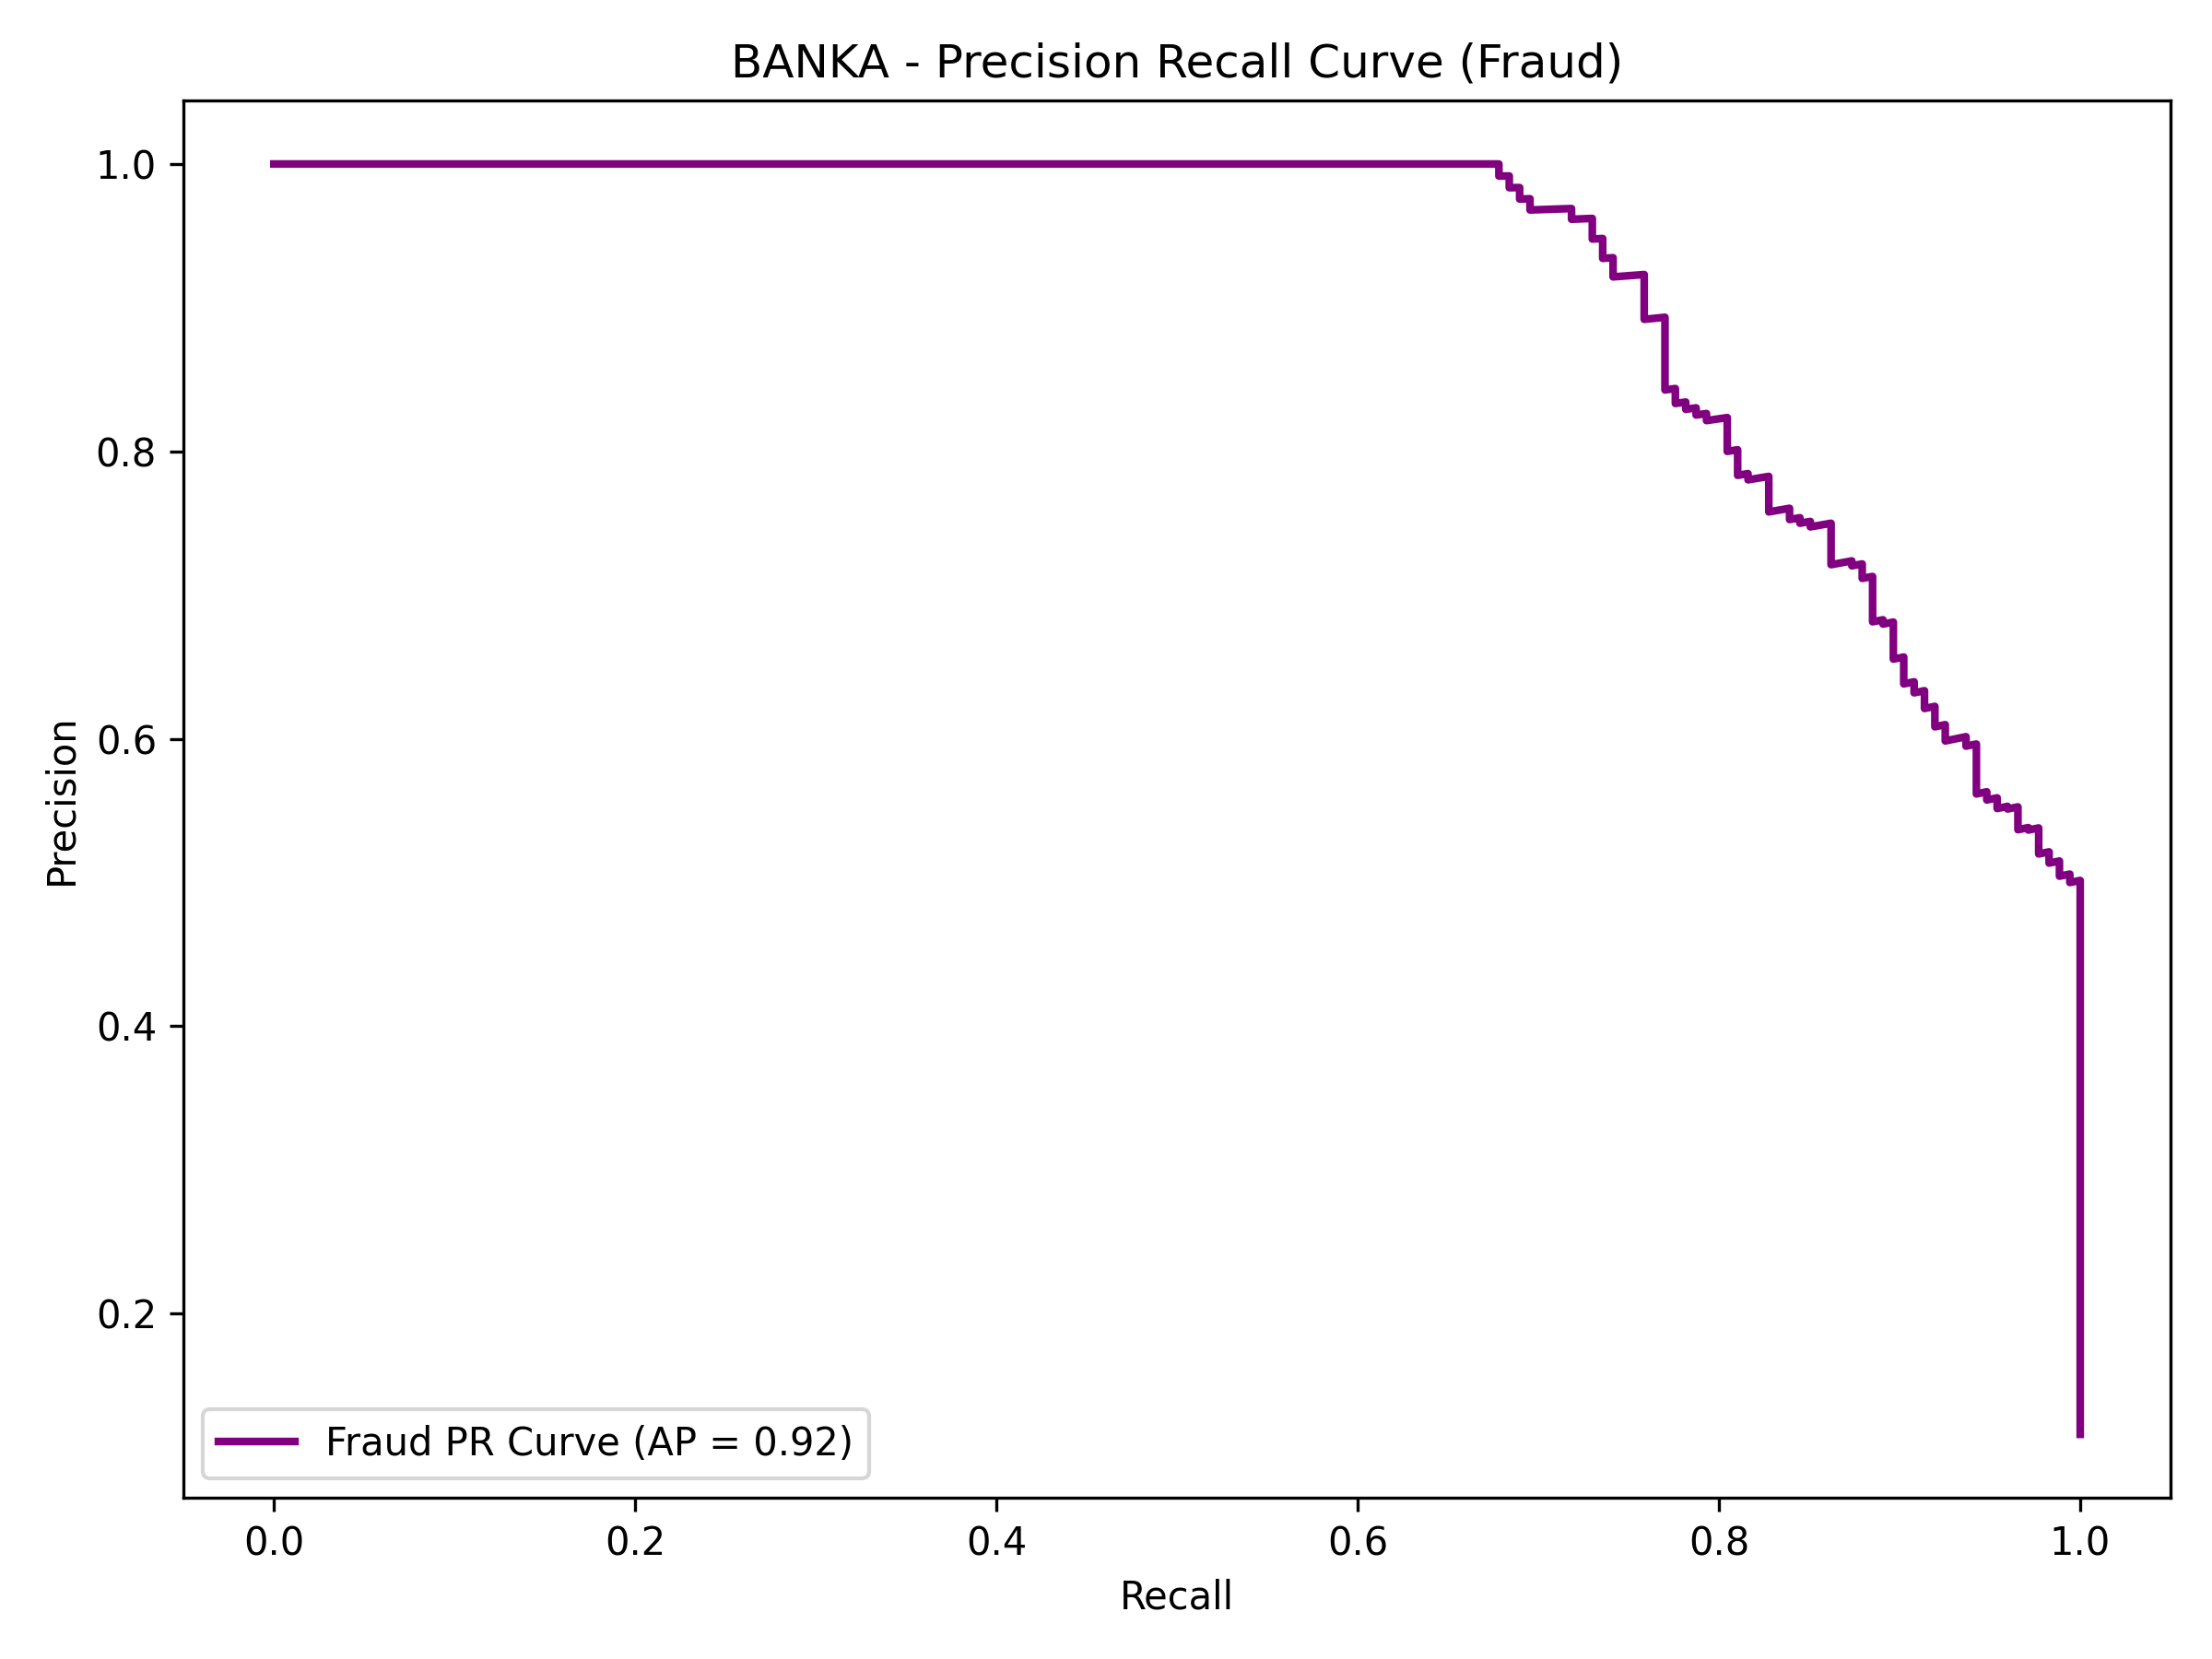
\includegraphics[width=\linewidth]{Figures/banka_pr_curve_deep.png}
\end{minipage}
\hfill
\begin{minipage}{0.48\textwidth}
\centering
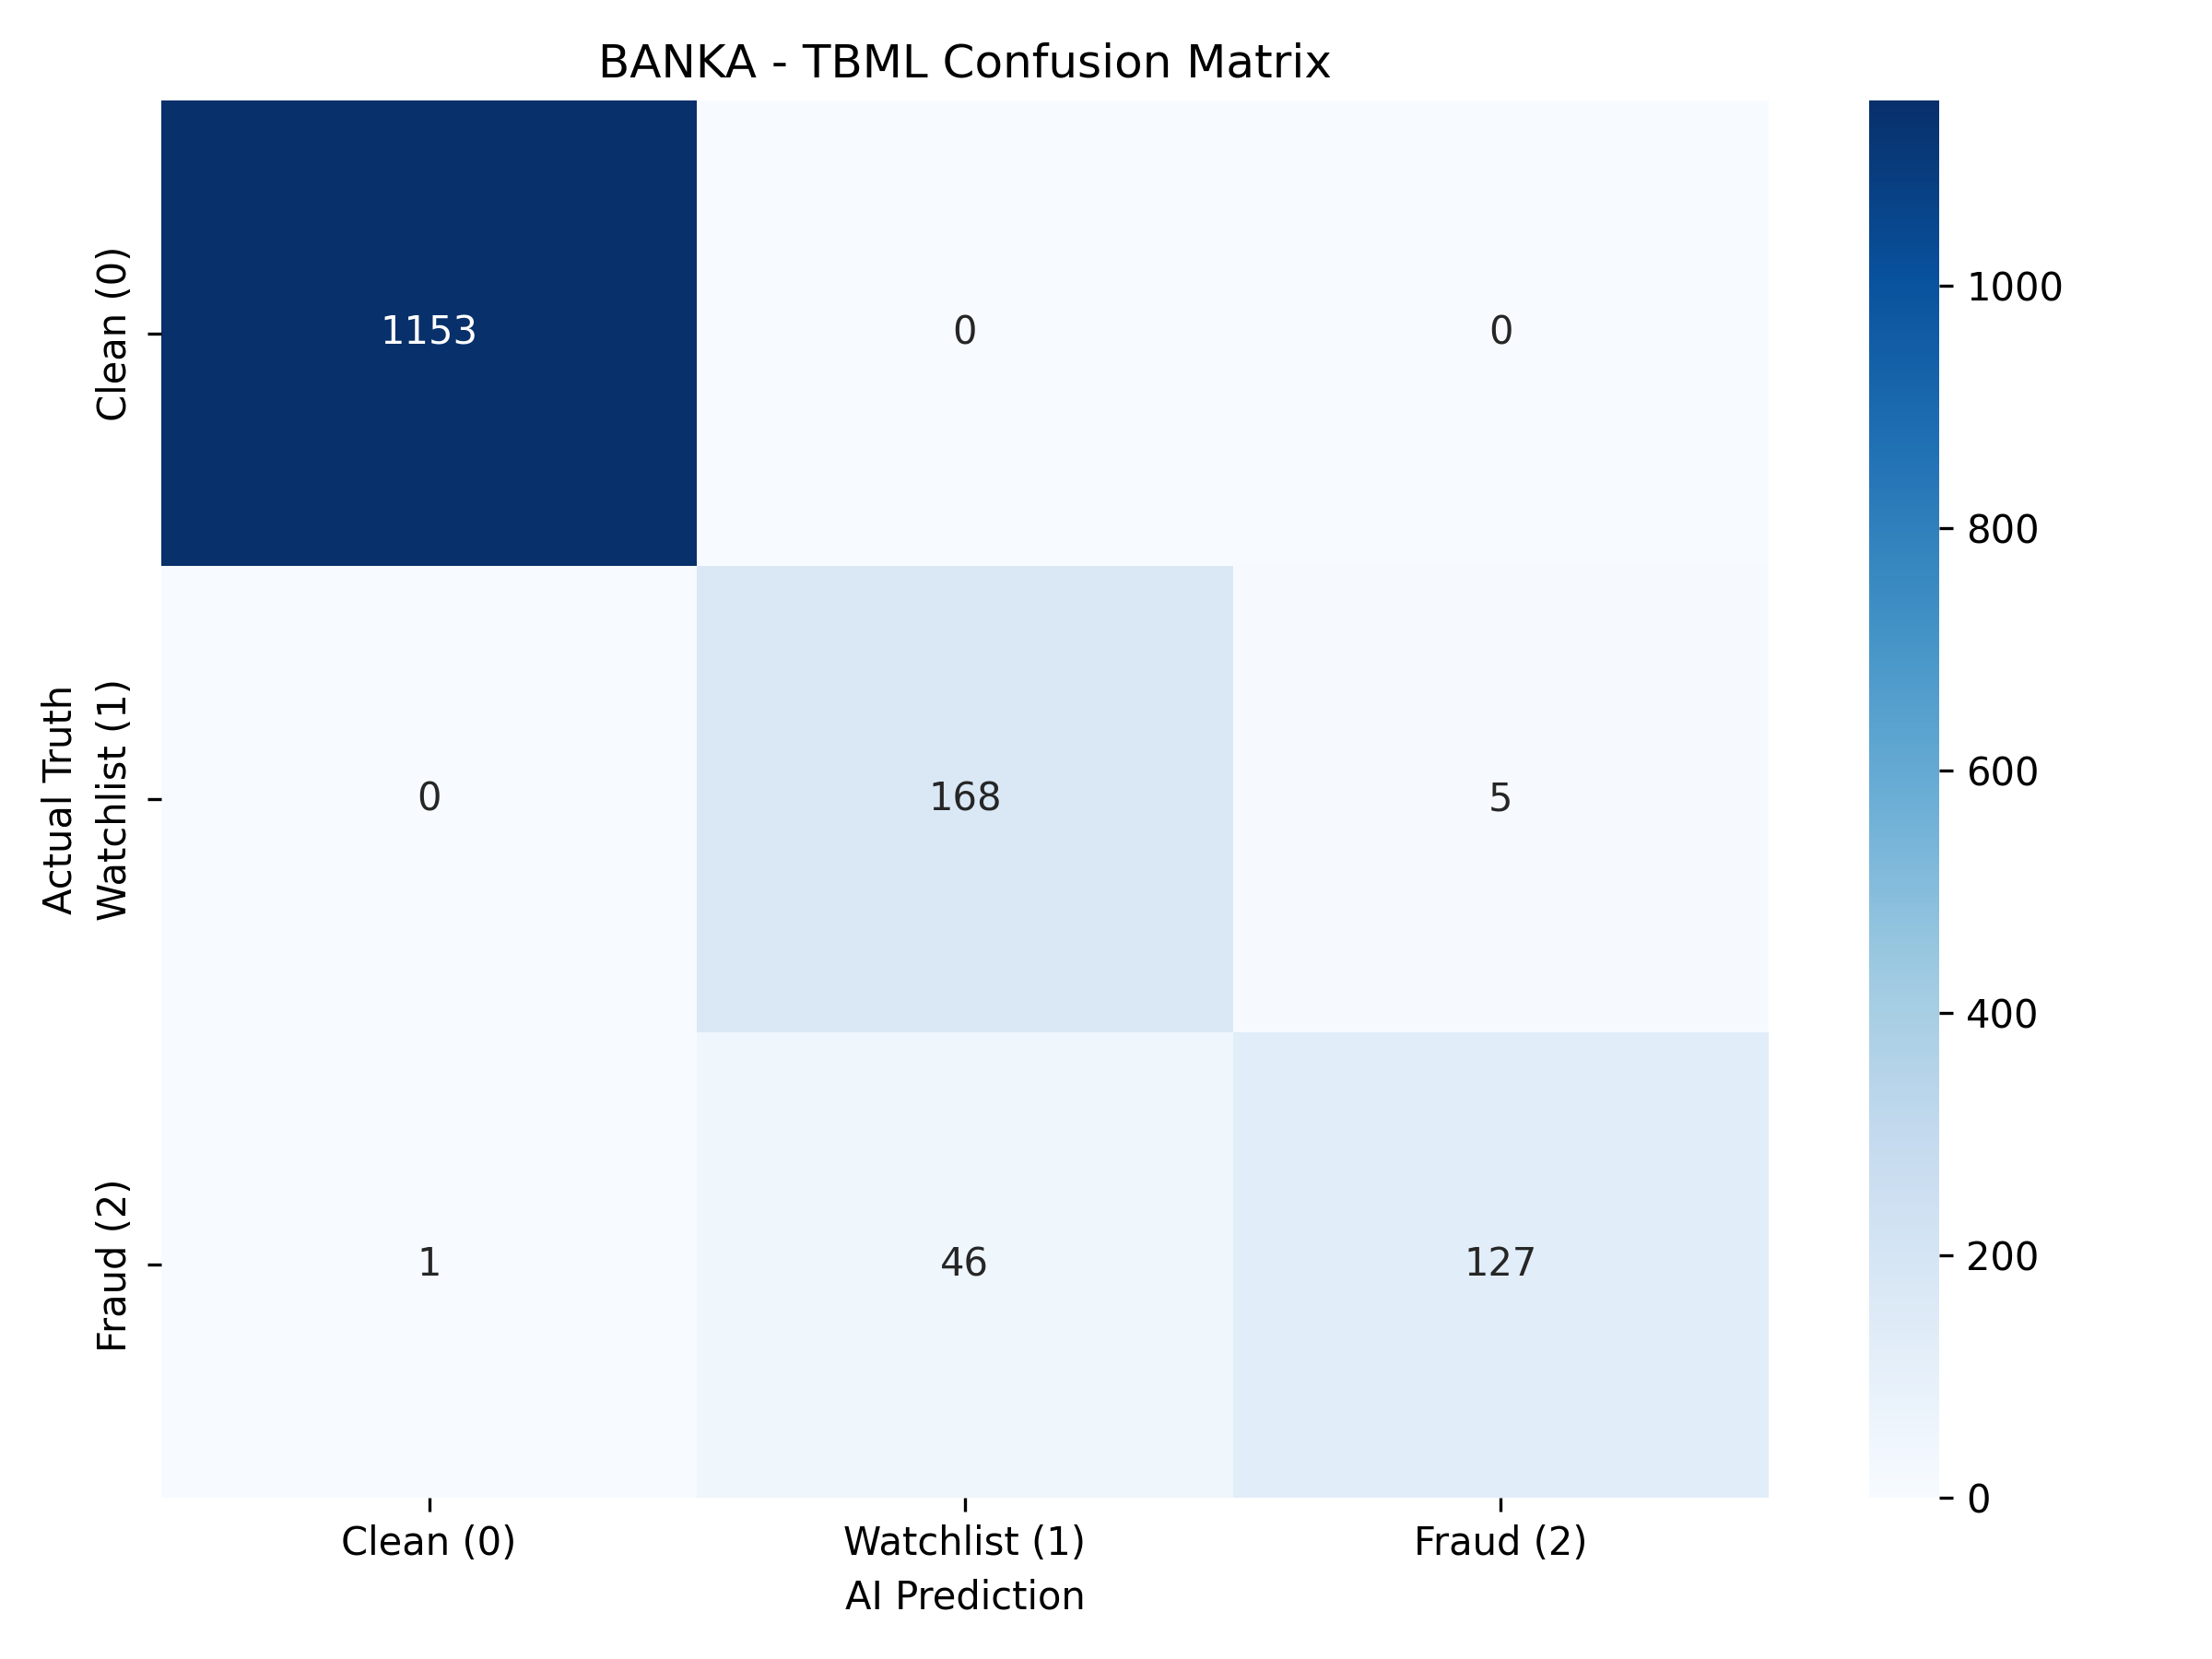
\includegraphics[width=\linewidth]{Figures/banka_confusion_matrix_deep.png}
\end{minipage}

\caption{BANKA Precision--Recall Curve and Confusion Matrix Validation}
\label{fig:banka_validation}
\end{figure}

As illustrated in Figure~\ref{fig:banka_validation}, the institutional environment of BANKA showed a highly
effective fraud-classification capacity, as measured by the Precision-Recall curve,
wherein the calculated Average Precision (AP) value amounted to about 0.92. The
curve showed highly precise detection at various levels of recall, reflecting an efficient
identification of the fraudulent transactional behavior even under class-imbalanced operational conditions. Additionally, the classification of Clean transactions proved perfect, as
no false positives were observed, and none of the transactions of this category was misclassified as fraud. Similarly, the classification of Watchlist transactions also showed a
high level of effectiveness, except for some instances that were classified as Fraud. In
addition, there was significant overlap between Fraud and Watchlist transactions,
where some of the transactions of the former category were classified as suspicious.
Nevertheless, the model kept its fraud-detection efficiency intact.

%--------------------------------------------------------
\subsection{BANKB Precision--Recall and Confusion Matrix Validation}
%--------------------------------------------------------

\begin{figure}[H]
\centering

\begin{minipage}{0.48\textwidth}
\centering
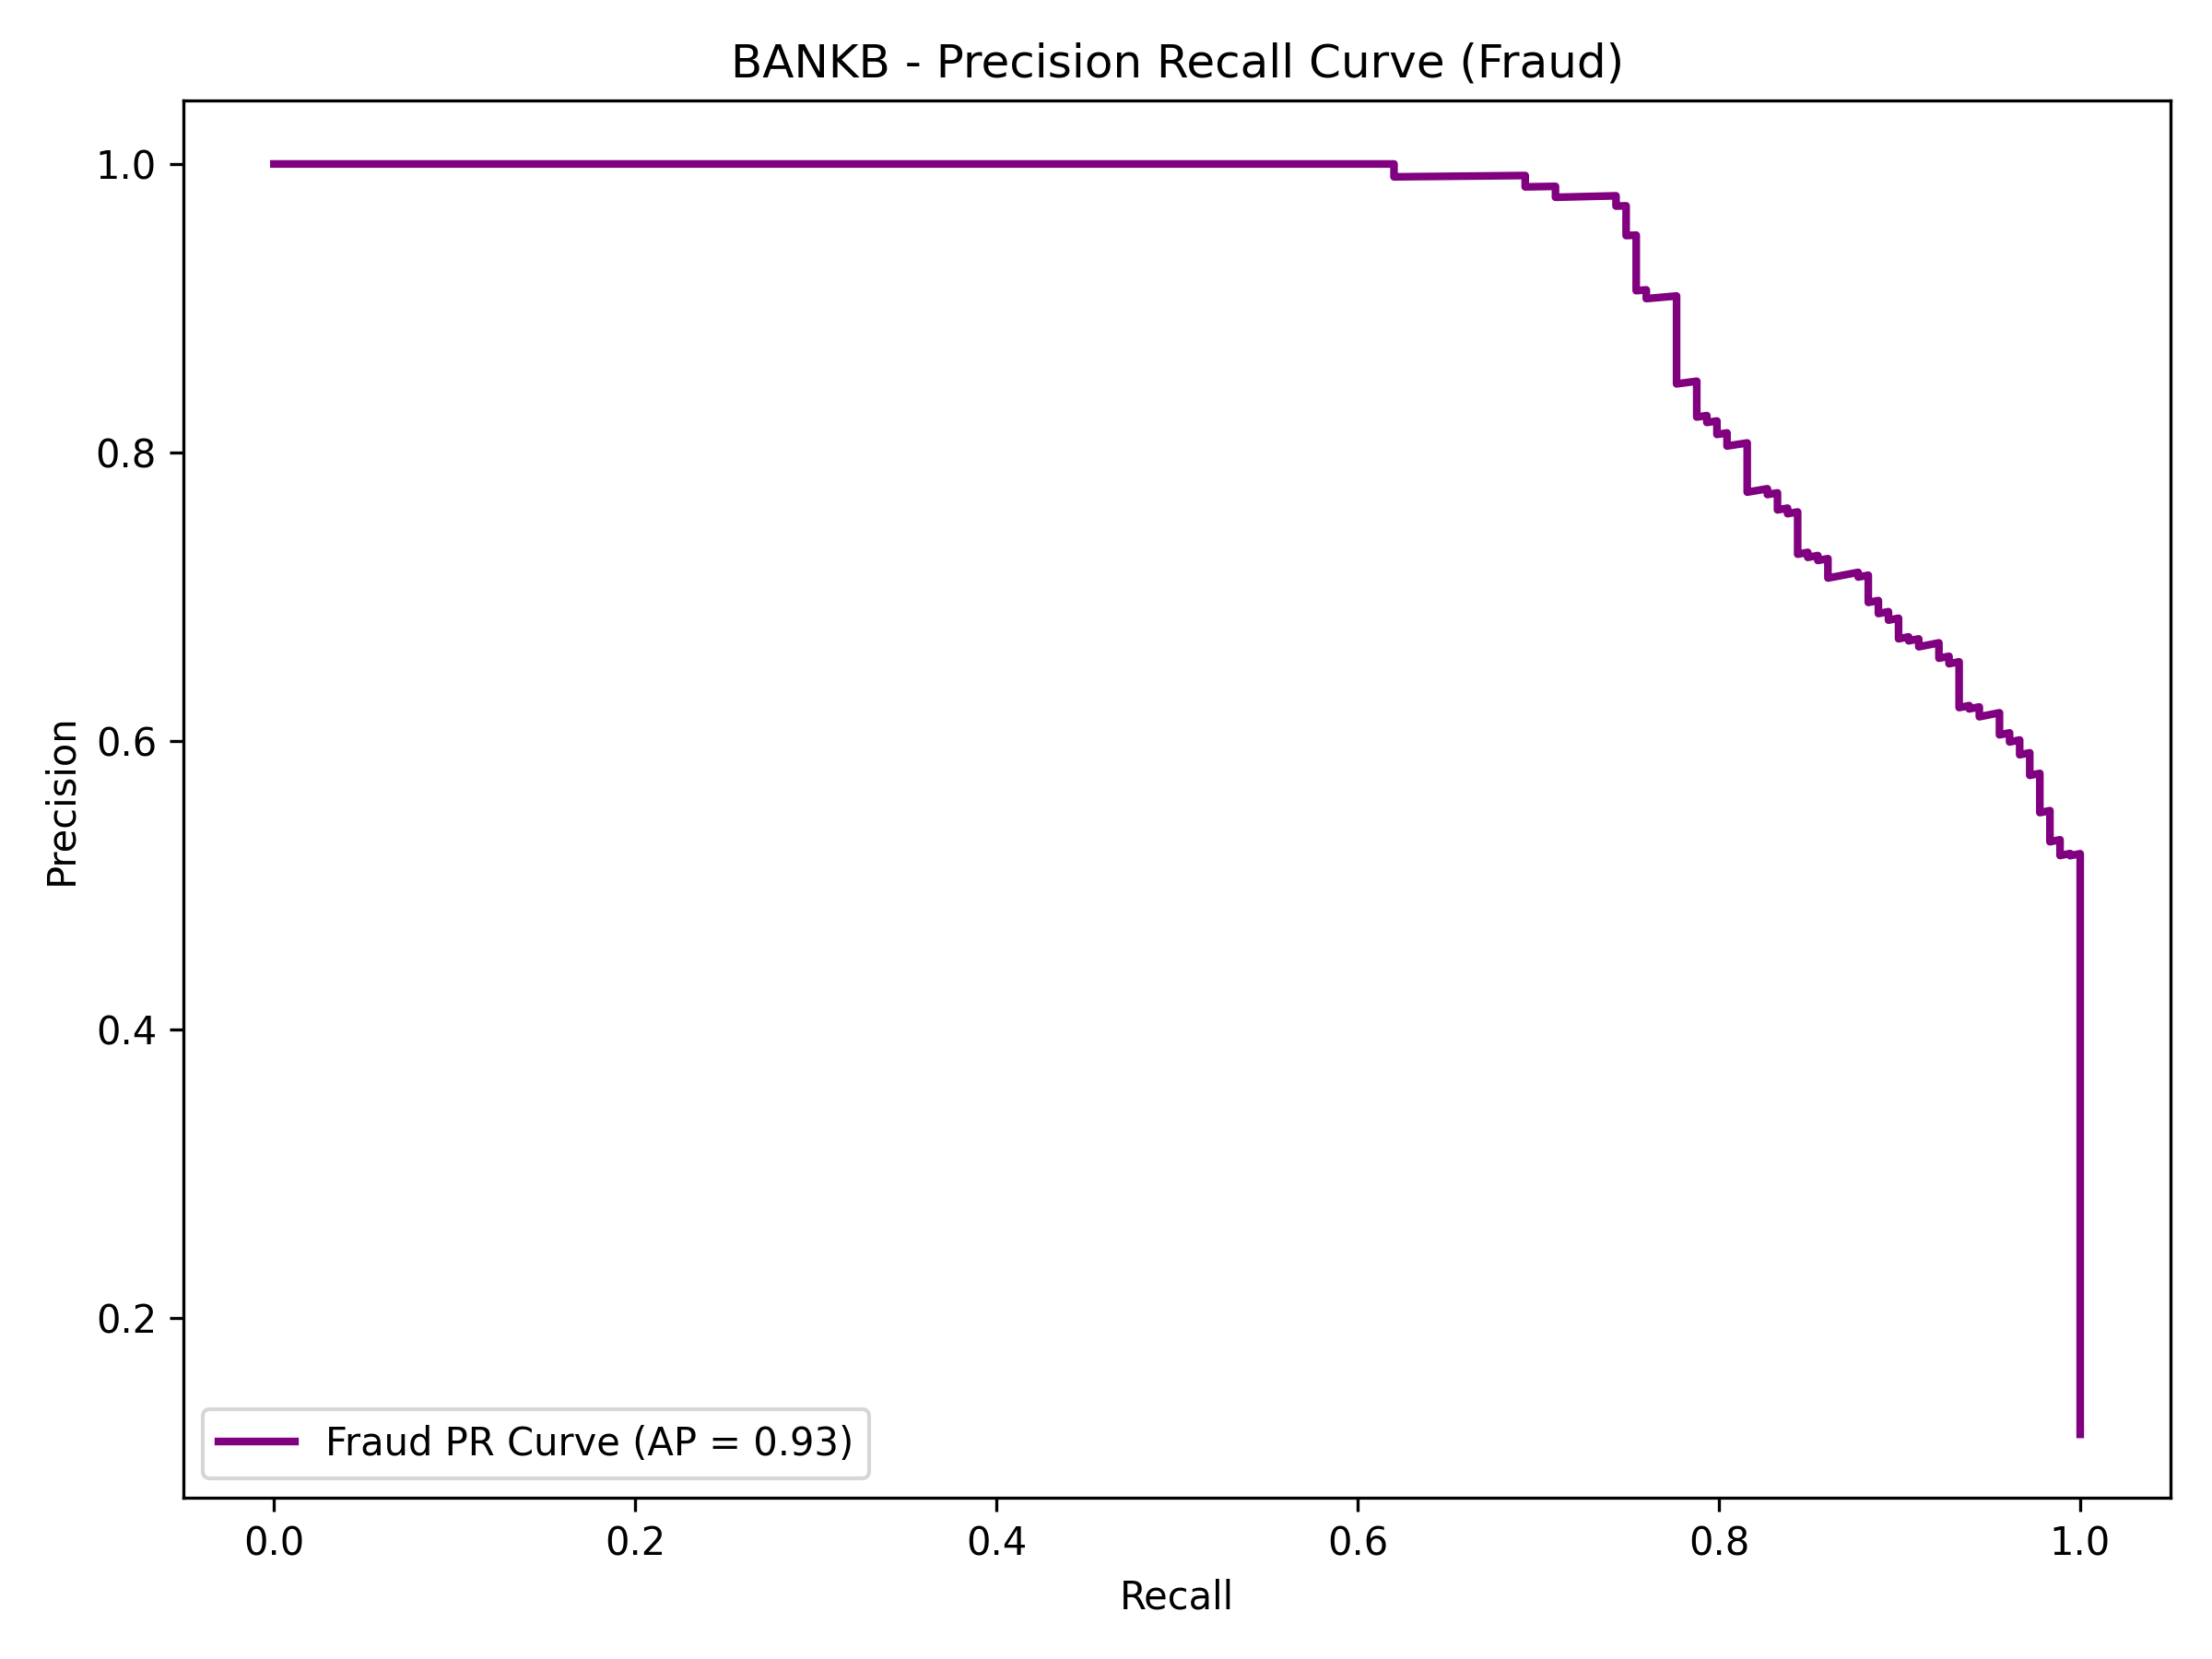
\includegraphics[width=\linewidth]{Figures/bankb_pr_curve_deep.png}
\end{minipage}
\hfill
\begin{minipage}{0.48\textwidth}
\centering
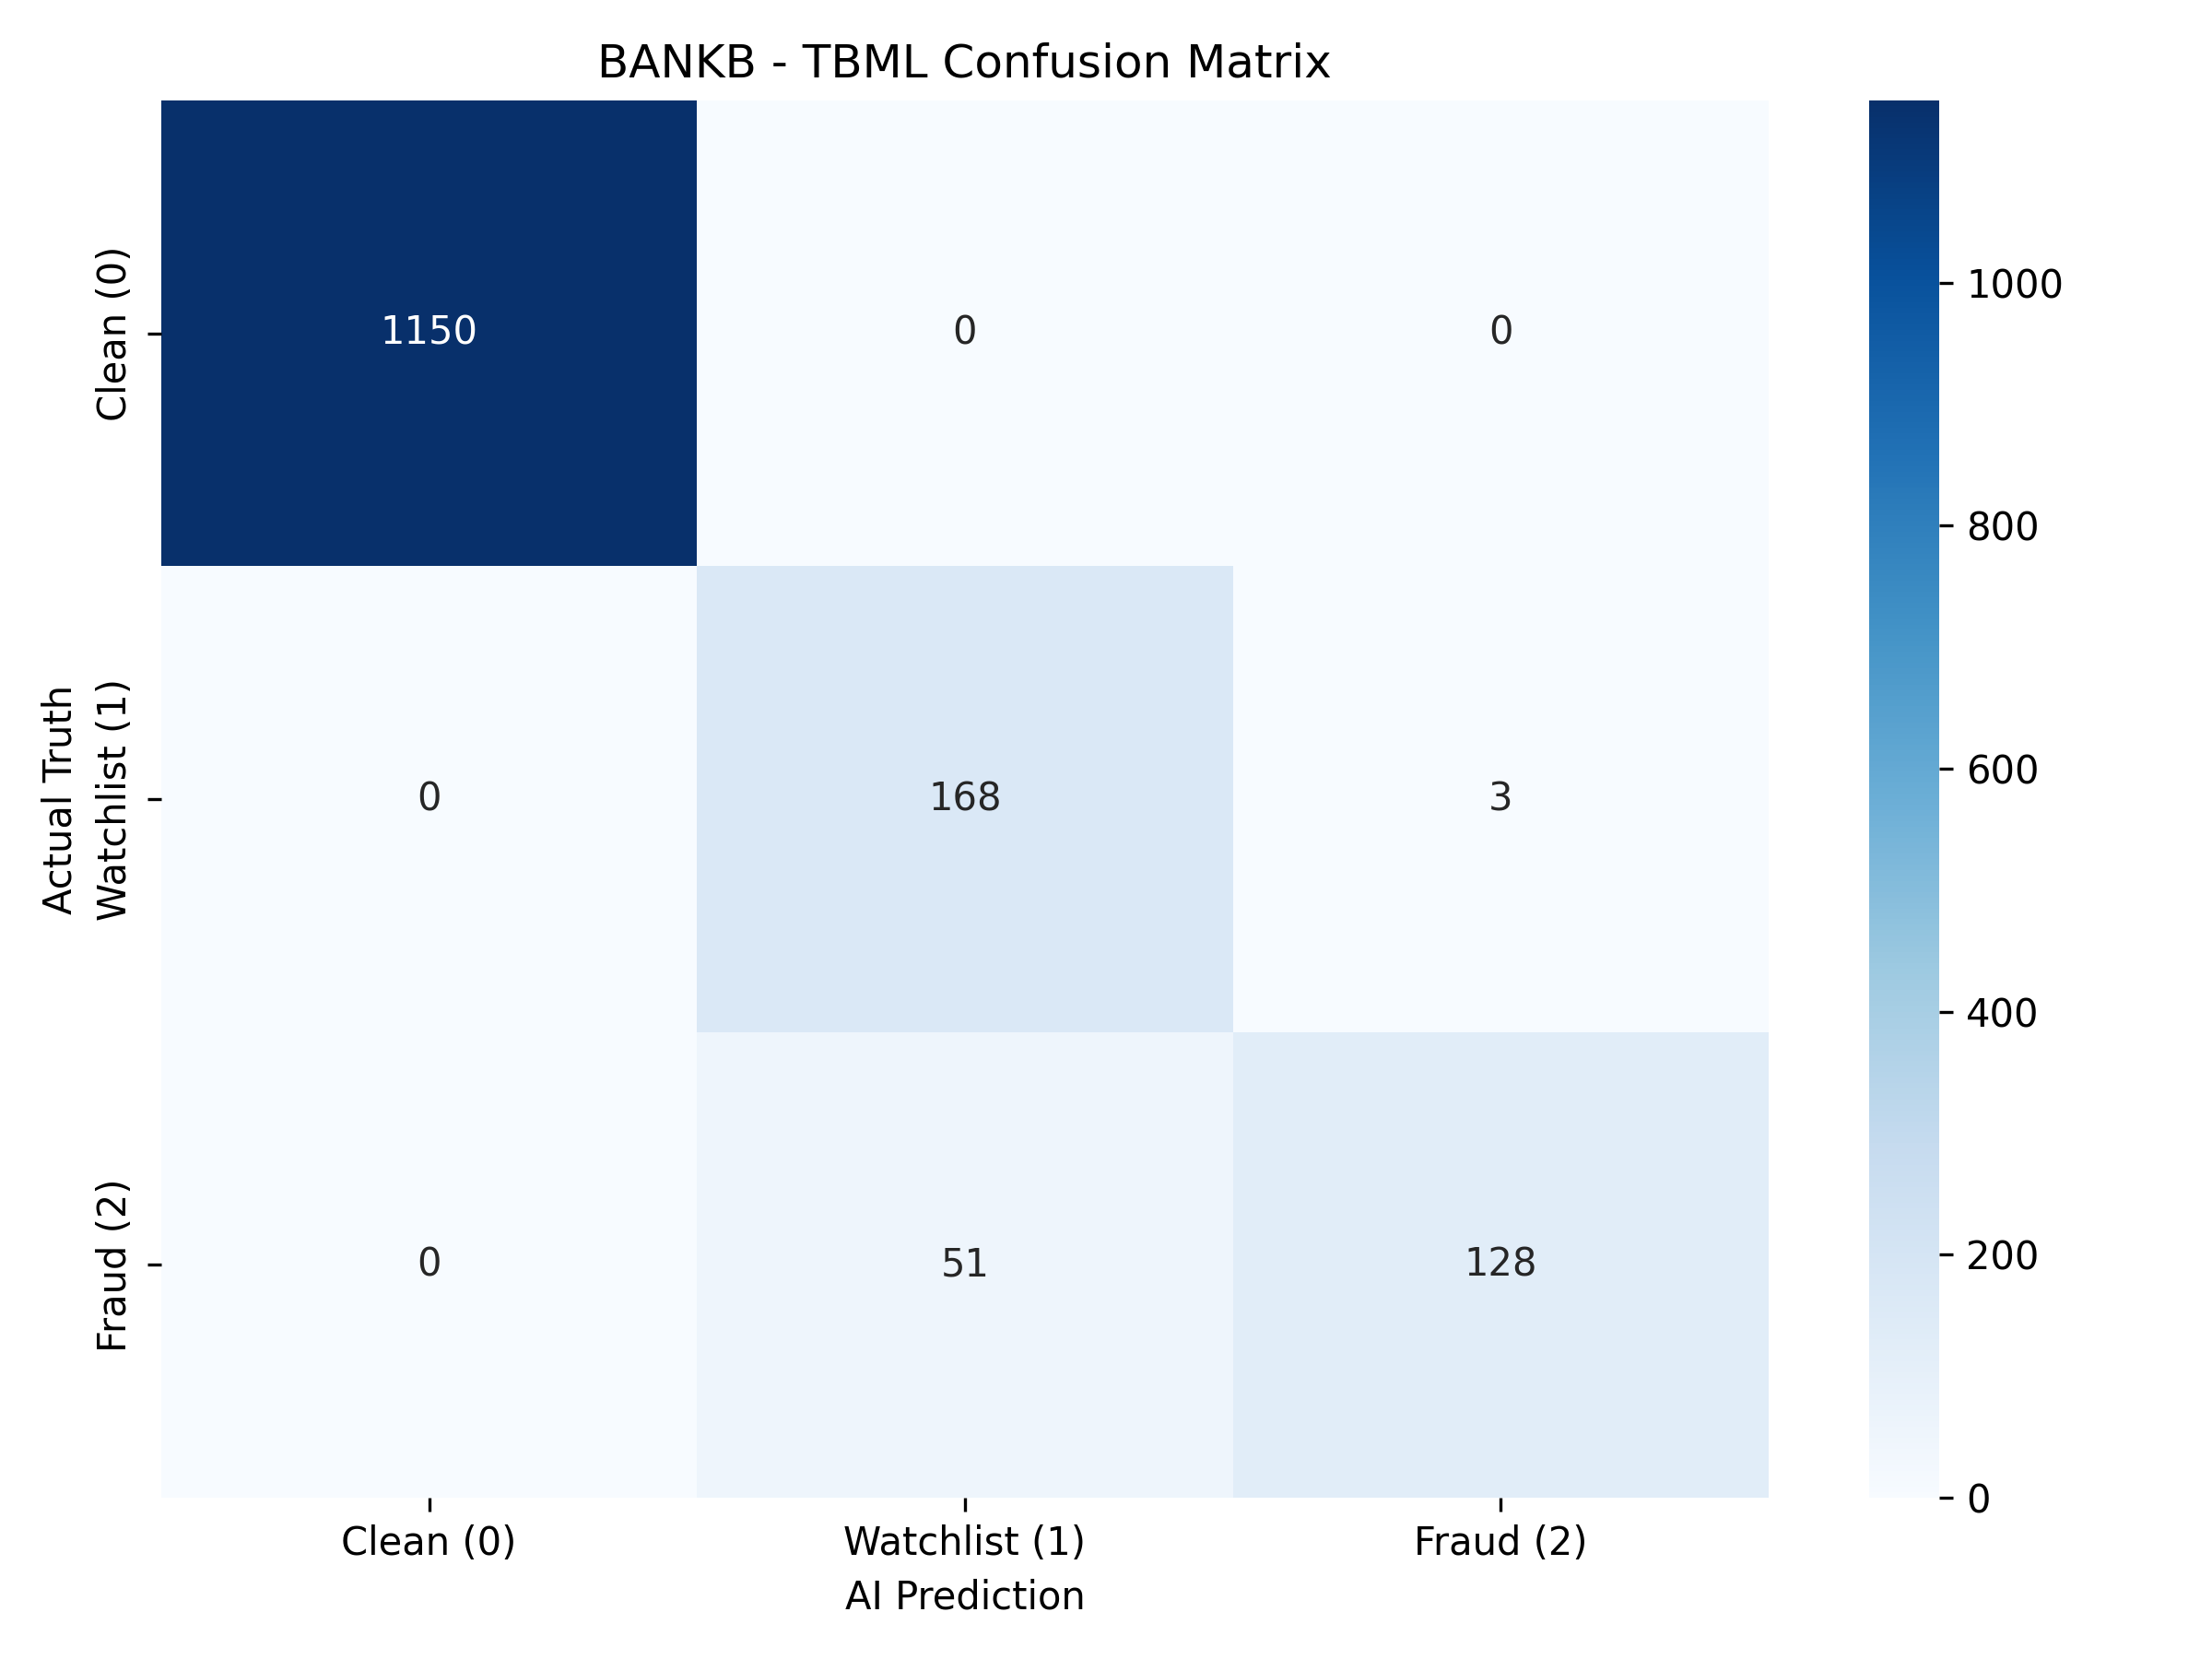
\includegraphics[width=\linewidth]{Figures/bankb_confusion_matrix_deep.png}
\end{minipage}

\caption{BANKB Precision--Recall Curve and Confusion Matrix Validation}
\label{fig:bankb_validation}
\end{figure}

As illustrated in Figure~\ref{fig:bankb_validation}, there was good fraud-classification ability within
the operational institutional environment of BANKB, because the generated Precision–Recall
curve resulted in a score of Average Precision (AP) that was equal to around 0.93.
The curve had kept high levels of precision for a wide range of the recall values,
thus, reflecting successful identification of fraud under conditions of class imbalance.
In its turn, the confusion matrix reflected excellent performance by showing perfectly
clean transaction class identification without making any false clean-to-fraud classification
errors. Transactions marked as "watchlist" were classified with high precision, while
only a few cases were mistakenly put into the Fraud class. As for the classification
overlap, it happened only for Fraud and Watchlist transaction classes, where some
transactions were classified as suspicious transactions. In spite of the overlap, fraud
detection ability remained sufficiently high. 



%========================================================
\subsection{BANKC Precision--Recall and Confusion Matrix Validation}
%--------------------------------------------------------

\begin{figure}[H]
\centering

\begin{minipage}{0.48\textwidth}
\centering
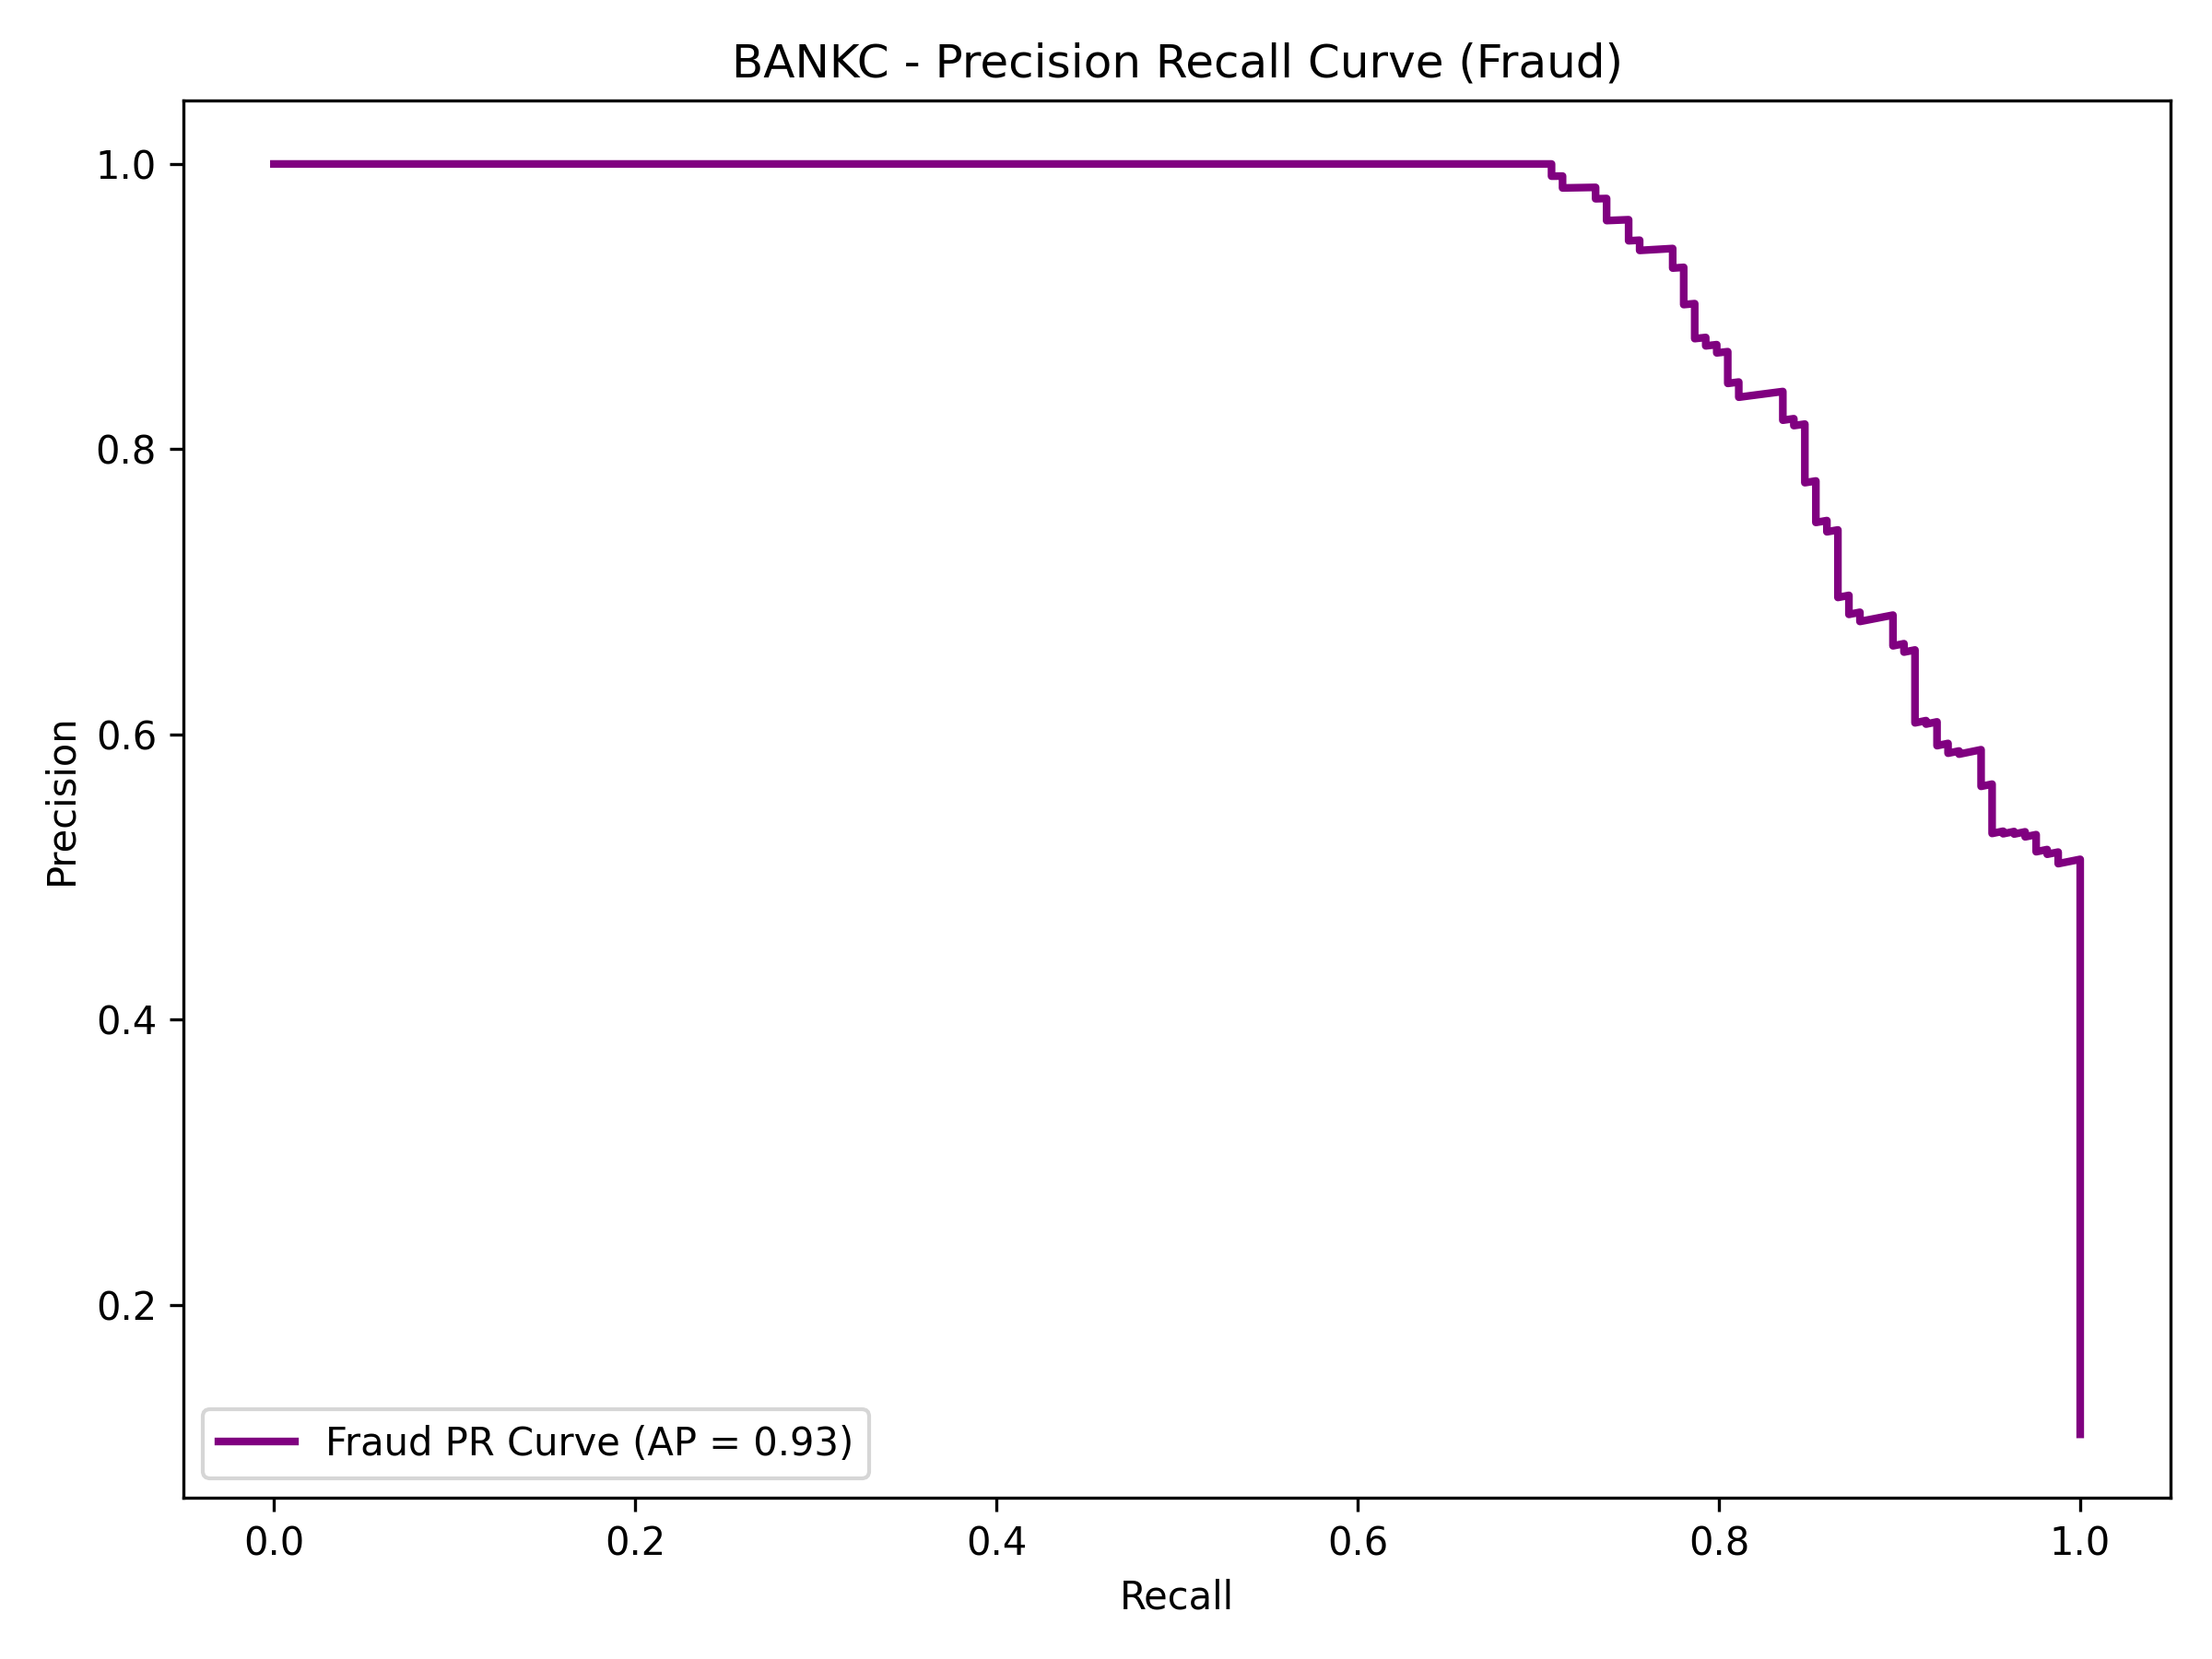
\includegraphics[width=\linewidth]{Figures/bankc_pr_curve_deep.png}
\end{minipage}
\hfill
\begin{minipage}{0.48\textwidth}
\centering
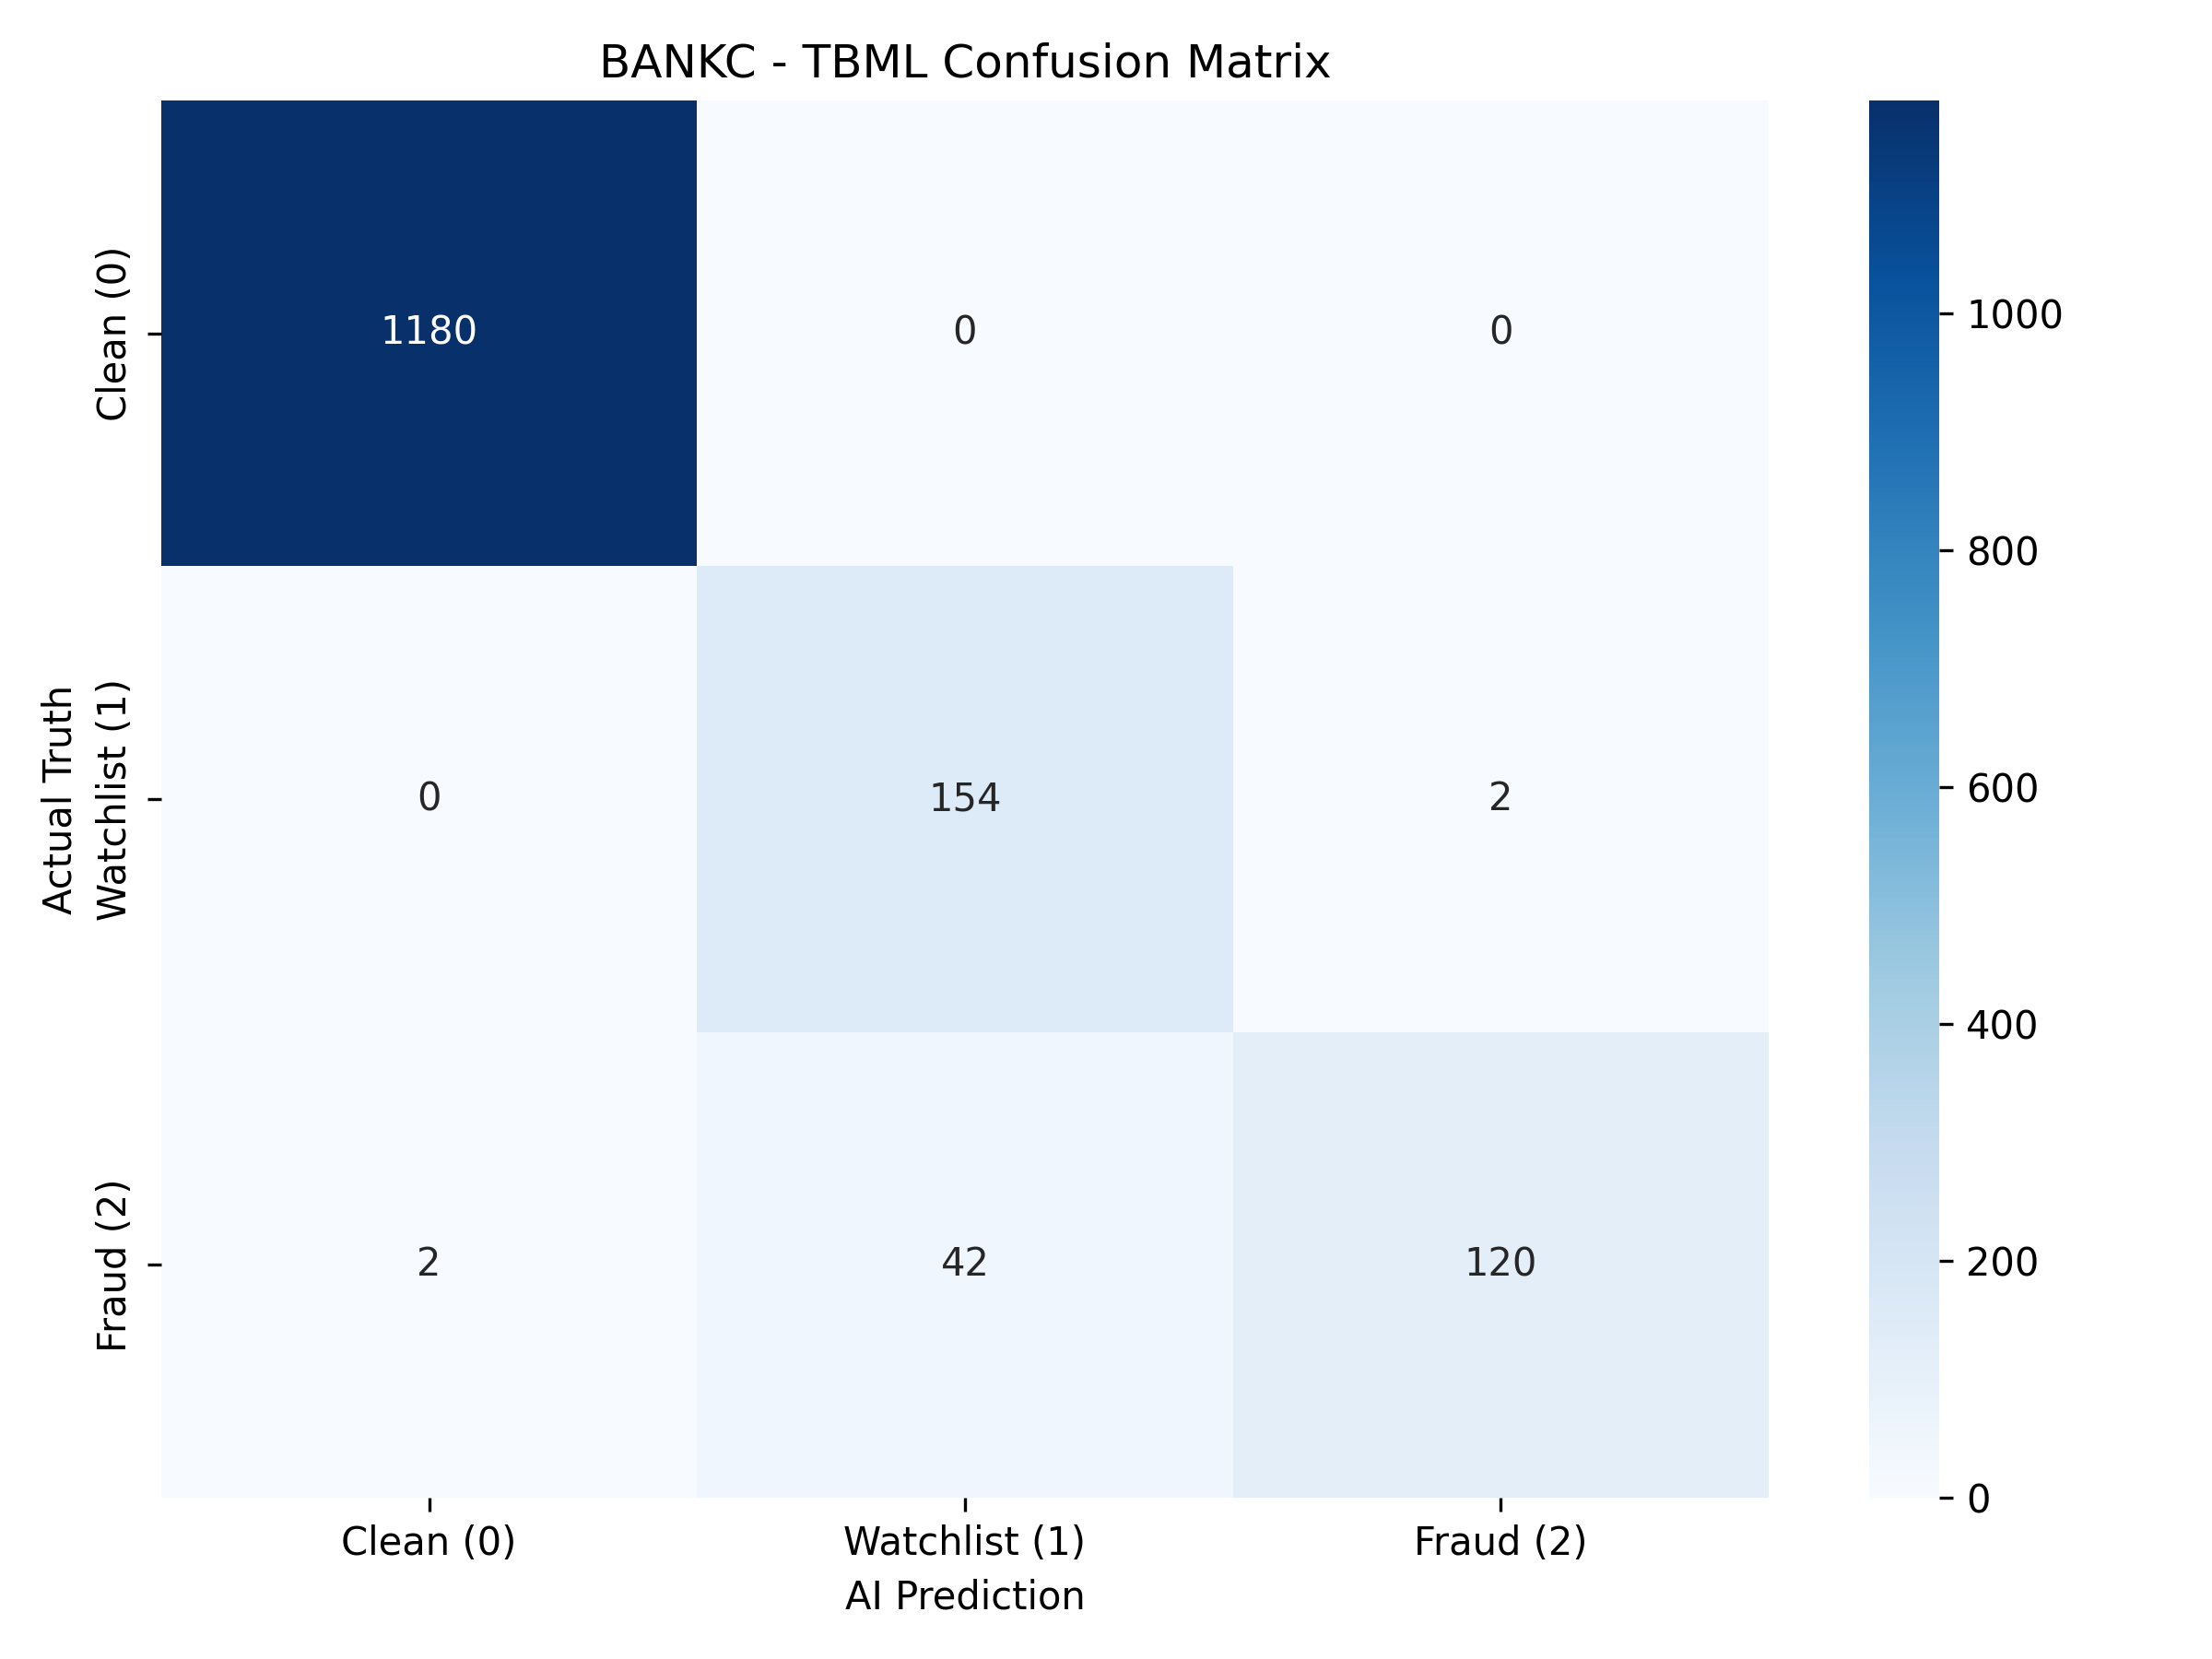
\includegraphics[width=\linewidth]{Figures/bankc_confusion_matrix_deep.png}
\end{minipage}

\caption{BANKC Precision--Recall Curve and Confusion Matrix Validation}
\label{fig:bankc_validation}
\end{figure}

As illustrated in Figure~\ref{fig:bankc_validation}, 
the precision-recall analysis shows that the BANKC
institutional environment exhibited great success in terms of classification of fraudulent
transactions, with the obtained Average Precision (AP) value amounting to roughly 0.93.
Furthermore, the graph showed excellent precision for various levels of recall, which is
indicative of the ability to detect fraudulent transactions under conditions of imbalanced
operating class environments. Additionally, perfect results for clean transactions can be
noted, as well as correct assignment of all suspicious transactions into their respective
transaction categories with no clean-to-fraud transactions. Finally, although there was
overlapping classification between watchlist and fraud categories (with some fraudulent
activities recognized as suspicious), the model successfully distinguished between the three
types of transactions in question.


\newpage
%========================================================
\section[Summary]{\textbf{Summary}}
%========================================================

This chapter validated the frameworks operational stability, synchronization reliability, and scalability across distributed institutional environments. Testing confirmed robust backend and graph-processing integration, secure transactional synchronization, and consistent dashboard performance under load. Model evaluation demonstrated strong multi-class discrimination, stable federated convergence, and reliable detection of suspicious and fraudulent transactions. The next chapter presents the detailed results and discussion.


		% % %Chapter 8
		%========================================================
\chapter{Results and Discussion}
%========================================================

This chapter presents the analytical outcomes and operational observations derived from experimental validation of the proposed federated Hybrid HGNN--LSTM framework for Trade-Based Money Laundering detection. Building upon the testing workflows discussed in Chapter 7, the following sections analyze the observed fraud-detection capability, federated learning stability, distributed synchronization behavior, and scalability characteristics of the deployed institutional monitoring framework.

%========================================================
\section[Overview of Experimental Outcomes]
{\textbf{Overview of Experimental Outcomes}}
%========================================================

The experimental evaluation demonstrated stable fraud-classification capability, reliable federated convergence behavior, and effective distributed synchronization across heterogeneous institutional transaction environments. The proposed framework successfully maintained multi-class analytical consistency for \textit{Clean}, \textit{Watchlist}, and \textit{Fraud} transaction states while preserving institutional data isolation during federated optimization workflows.

The distributed streaming and graph-processing architecture additionally enabled synchronized real-time transaction propagation, stable heterogeneous graph generation, and controlled dashboard-update behavior during concurrent monitoring workflows. System-level scalability evaluation further demonstrated stable PostgreSQL query execution, efficient transaction persistence, and controlled API response latency under increasing institutional monitoring workloads.

%========================================================
\section[Operational Performance Outcomes]
{\textbf{Operational Performance Outcomes}}
%========================================================

The deployed monitoring framework demonstrated stable operational performance across distributed fraud-monitoring and compliance-management workflows. Dashboard transaction retrieval, fraud filtering, STR synchronization, and regulator-side compliance propagation maintained reliable execution consistency under concurrent institutional workloads. Table~\ref{tab:operational_metrics} summarizes the observed API-level operational response characteristics across major compliance workflows.

\begin{table}[H]
\centering
\caption{Operational Workflow Performance Summary}
\vspace{0.2cm}

\renewcommand{\arraystretch}{1.3}

\begin{tabular}{|p{4.5cm}|p{2.5cm}|p{2.8cm}|p{2.3cm}|}
\hline
\textbf{Workflow} & \textbf{Avg Response Time} & \textbf{Operational Observation} & \textbf{Status} \\ \hline

Dashboard Transaction Retrieval
& $\sim160$ ms
& Stable under concurrent workloads
& Successful \\ \hline

Fraud Transaction Filtering
& $\sim148$ ms
& Controlled query latency during filtering
& Successful \\ \hline

STR Compliance Retrieval
& $\sim466$ ms
& Stable relational aggregation behavior
& Successful \\ \hline

STR Generation Workflow
& $<1$ s
& Successful compliance synchronization
& Successful \\ \hline

Notification Propagation
& $<500$ ms
& Stable regulator-side synchronization
& Successful \\ \hline

Federated Fraud Inference
& $\sim1$--$2$ s
& Stable graph-based analytical prediction
& Successful \\ \hline

\end{tabular}

\renewcommand{\arraystretch}{1}

\label{tab:operational_metrics}
\end{table}

As observed in Table~\ref{tab:operational_metrics}, dashboard synchronization and fraud-filtering workflows maintained comparatively low response latency during concurrent institutional workloads. The STR retrieval workflow exhibited comparatively higher latency due to computationally intensive relational joins, transaction-history aggregation, and compliance-report synchronization operations executed during report-generation workflows. However, stable response consistency and successful request execution were maintained across all monitored operational workflows.

%========================================================
\section[Graph-Based TBML Detection Capability]
{\textbf{Graph-Based TBML Detection Capability}}
%========================================================

The graph-based analytical workflow demonstrated strong capability in learning hidden transactional dependencies and multi-hop entity relationships across heterogeneous institutional transaction environments. Unlike traditional rule-based AML systems that primarily depend on isolated transactional heuristics, the proposed framework leveraged heterogeneous graph construction to capture interconnected relationships between accounts, SWIFT transactions, trade metadata, compliance documents, and institutional entities during fraud-inference workflows.

The confusion-matrix evaluation discussed in Chapter 7 demonstrated that most classification overlap occurred between \textit{Watchlist} and \textit{Fraud} transaction states, while minimal propagation of fraudulent predictions into legitimate transactional categories was observed. This behavior validated the effectiveness of graph-topology learning for identifying suspicious transactional relationships without excessively escalating legitimate institutional transactions into fraud classifications during compliance-monitoring operations.

%========================================================
\section[Federated Learning Effectiveness]
{\textbf{Federated Learning Effectiveness}}
%========================================================

The federated analytical workflow demonstrated stable distributed convergence behavior across all participating institutional clients during iterative FedAvg synchronization operations. The convergence progression analyzed in Chapter 7 showed gradual stabilization of Accuracy, Precision, and Recall metrics during later federated communication rounds, thereby validating effective distributed parameter synchronization and stable institutional knowledge sharing during collaborative optimization workflows.

Table~\ref{tab:federated_results} summarizes the observed federated analytical performance across distributed institutional clients after completion of iterative global aggregation workflows.

\begin{table}[H]
\centering
\caption{Federated Analytical Performance Summary}
\vspace{0.2cm}

\renewcommand{\arraystretch}{1.3}

\begin{tabular}{|p{2.2cm}|p{2.2cm}|p{2cm}|p{2cm}|p{2cm}|}
\hline
\textbf{Institution} & \textbf{Transaction Class} & \textbf{Precision} & \textbf{Recall} & \textbf{F1-Score} \\ \hline

BANKA
& Fraud (2)
& 0.96
& 0.73
& 0.83 \\ \hline

BANKB
& Fraud (2)
& 0.98
& 0.73
& 0.84 \\ \hline

BANKC
& Fraud (2)
& 0.98
& 0.73
& 0.84 \\ \hline

\end{tabular}

\renewcommand{\arraystretch}{1}

\label{tab:federated_results}
\end{table}

As observed in Table~\ref{tab:federated_results}, the federated Hybrid HGNN--LSTM framework maintained high Fraud-class Precision across all participating institutional environments while preserving stable Recall characteristics during distributed analytical inference. The observed convergence stability additionally indicated that the proposed framework successfully generalized fraud-learning behavior across heterogeneous institutional transaction environments without requiring centralization of sensitive transactional datasets.

%========================================================
\section[Real-Time Monitoring and Compliance Outcomes]
{\textbf{Real-Time Monitoring and Compliance Outcomes}}
%========================================================

The distributed transaction-monitoring workflow demonstrated stable real-time synchronization of institutional transaction streams across heterogeneous backend analytical services. Kafka-based asynchronous event propagation enabled continuous ingestion of SWIFT transactional payloads into downstream graph-construction and federated inference pipelines without interrupting institutional monitoring workflows.

The automated STR generation and notification workflow additionally improved operational coordination between banking institutions and regulator-facing compliance environments. Fraud-classified transactional events were successfully transformed into structured compliance reports while preserving associated transaction histories, graph metadata, and institutional investigation references during distributed monitoring operations.


%========================================================
\section[Scalability and Infrastructure Observations]
{\textbf{Scalability and Infrastructure Observations}}
%========================================================

Concurrent scalability evaluation demonstrated stable API response behavior and reliable PostgreSQL synchronization consistency under increasing institutional monitoring workloads. During dashboard transaction retrieval workflows, the framework maintained average response latencies near $156$--$162$ ms across concurrent workloads ranging from 50 to 500 users while sustaining complete request success rates throughout the evaluation process. Similarly, fraud-transaction filtering workflows maintained average response latency near $148$--$159$ ms under moderate concurrent workloads, thereby validating stable pooled-query execution and controlled backend synchronization during real-time monitoring operations.

The STR compliance retrieval workflow exhibited comparatively higher computational latency due to relational joins, transaction-history aggregation, and regulator-side compliance synchronization executed during report-generation workflows. Initial average response latency near $2694$ ms during lower concurrent execution stages progressively reduced to nearly $466$ ms during higher concurrent workloads, thereby indicating improved query-plan stabilization, PostgreSQL shared-buffer utilization, and optimized relational-query execution during repeated compliance-retrieval operations. Despite occasional tail-latency spikes during high-concurrency execution stages, the infrastructure evaluation maintained stable request consistency and complete request success rates throughout distributed monitoring and compliance-management workflows.
%========================================================
\section[Comparative Architectural Advantages]
{\textbf{Comparative Architectural Advantages}}
%========================================================

The proposed federated Hybrid HGNN--LSTM framework demonstrated several operational and analytical advantages over traditional rule-based AML monitoring systems. Conventional compliance frameworks primarily depend on manually engineered heuristics and isolated threshold-based transaction analysis, thereby limiting their capability to identify hidden multi-hop transactional relationships and evolving laundering topologies embedded within large-scale institutional trade networks.

In contrast, the proposed framework enabled graph-based relational inference across interconnected transactional entities while simultaneously preserving institutional data isolation through decentralized federated synchronization. The integration of real-time streaming, distributed graph processing, federated optimization, and automated compliance orchestration therefore provided significantly improved operational monitoring capability compared to conventional static AML investigation workflows.

%========================================================
\section[Summary]
{\textbf{Summary}}
%========================================================

The experimental outcomes and analytical observations validated the effectiveness of the proposed federated Hybrid HGNN--LSTM framework for distributed Trade-Based Money Laundering detection and compliance monitoring. The observed results demonstrated stable graph-based fraud inference, reliable federated convergence behavior, controlled scalability characteristics, and effective real-time synchronization across distributed institutional monitoring environments. The framework additionally achieved privacy-preserving collaborative learning without requiring centralization of sensitive transactional datasets, thereby validating its operational suitability for large-scale institutional compliance ecosystems.

		% %Chapter 9
		%========================================================
\chapter{Conclusion}
%========================================================

This study presents an efficient implementation of the scalable and secure fed
erated graph learning framework for the intelligent TBML detection within distribu ted institutional environments. The designed framework included hetero geneous graph learning, federated Hybrid HGNN-LSTM analytical inference, Apache Kafka-based transaction processing, PostgreSQL-based compli ance orchestration, and regulator-oriented monitoring synchronization within the consoli dated infrastructure. Stable performance in terms of the Fraud-class Precision near 0.98 and reliable federated learning behavior was demonstrated through the experimenta l evaluation of the proposed framework. In addition, concurrent scalability experiments
proved stability in dashboard latency near 156-162 ms and fraud-filtering latenc y near 148-159 ms under gradually increasing monitoring load. All these outcomes pro ve the ability of the proposed framework to perform TBML detection within distri buted institutional environments reliably, scalably, and securely.

%========================================================
\section{Limitations}
%========================================================
In spite of stable analytical performance and effective monitoring capability, there are
some practical limitations associated with the current implementation of the proposed
framework. In particular, experimental results were obtained based on the synthetic
enrichment of institutional transactional datasets due to the lack of institution ally verified TBML datasets annotated with laundering activities. As a consequence, some laundering behaviors and trade manipulation practices might not be sufficiently repre sented within the present experimental environment.

 The federated workflow also results in increased communication costs while
synchronizing parameters in a distributed manner. The synchronization costs may be pro
portionally higher with an increasing number of participating banking environments. In
the same way, the graph-processing workflow involving large banking transaction envi
ronments may cause extra computational costs in the context of high-throughput mul
ti-hop graph traversal and distributed inference operations.
Fraud detection, monitoring, and compliance notification are the primary applica
tions covered by our current system. Although the framework provides effective support
for alert propagation and coordination within regulatory institutions and among institu
tional participants, no automated action mechanisms (such as transaction blocking,
account freezing, document locking, and dynamic compliance triggers) are considered in
the framework, requiring closer coupling with banking infrastructure.

%========================================================
\section{Future Scope}
%========================================================
There are still several possibilities for further scaling up the suggested framework to more production-ready and scalable financial crime-monitoring ecosystems. A future research area would be to test the framework with more institutionally-backed TBML datasets, with real-world laundering annotations, cross-border laundering behaviors and increasingly changing topologies in the financial crime domain. These datasets will enhance the robustness of the analytical and the operational generalisation in large scale banking environments.

In further extensions, the semantic representation extraction system from unstructured trade documents such as invoices, customs declarations, shipping documents, and letters of credit may be implemented using a transformer architecture. These context-specific embeddings can then be combined into the graph-learning process to enhance semantic anomaly detection and trade-document authentication steps. The federated learning ecosystem could also expand to geographically distributed banking ecosystems with more widespread and larger institutional participation.

Future implementations may also utilize enhanced secure aggregation methods like Fully Homomorphic Encryption (FHE), Secure Multi-Party Computation (SMPC), and differential privacy methods to further bolster the security of distributed parameter synchronization operations against gradient-leakage and model-inversion attacks. There is also potential for further research on Continuous-Time Dynamic Graph (CTDG) architectures, in addition to the use of explainable graph neural networks (XGNNs) to further enhance the temporal topology tracking and graph-level interpretability for institutional compliance analysts.

This proposed solution can also be developed into an end-to-end banking compliance solution. In addition to fraud detection and propagation of notifications, future deployments can enable automated compliance-response orchestration, such as freezing transactions, executing risk triggers as per the regulators' requirements, verifying documents from institutions, implementing regulator-approved intervention pipelines, and restricting accounts based on policies embedded in core banking systems.
%========================================================
\section{Learning Outcomes of the Project}
%========================================================

% \begin{itemize}

% \item Acquired practical experience in designing and deploying heterogeneous graph-learning architectures for large-scale financial fraud-detection workflows.

% \item Developed understanding of federated learning environments, distributed parameter synchronization, and privacy-preserving collaborative analytical inference across institutional systems.

% \item Gained hands-on exposure to real-time streaming architectures using Apache Kafka, asynchronous backend synchronization, and distributed event-driven monitoring workflows.

% \item Learned implementation and optimization of graph neural networks, temporal sequence modeling, and multi-modal feature fusion for fraud-classification tasks.

% \item Developed expertise in PostgreSQL database optimization, concurrent API scalability analysis, connection pooling, and distributed compliance-management synchronization workflows.

% \item Acquired experience in full-stack system integration involving Next.js dashboards, Prisma ORM synchronization, authentication workflows, and regulator-facing monitoring environments.

% \item Gained understanding of operational AML workflows including STR lifecycle management, compliance orchestration, fraud-notification propagation, and institutional investigation coordination.

% \item Learned experimental benchmarking, model-performance evaluation, Precision--Recall analysis, confusion-matrix interpretation, and distributed scalability validation for real-time analytical systems.

% \end{itemize}

The suggested TBML detection system introduced practical experience with het
erogenous graph-learning models, federated learning platforms, and real-time financial
fraud-detection systems. The project gave practical experience working with Graph Neural Net
works, time sequence analysis, synchronized model parameters training, and data infer
ence using privacy-preserving analytics. Moreover, practical knowledge was obtained re
lated to Apache Kafka real-time stream processing, PostgreSQL database manage
ment, scalability evaluation of an API, and end-to-end application development using
Next.js, Prisma ORMs, and FastAPI. Also, practical skills were developed concerning
AML compliance processes, STR lifecycle, fraud detection monitoring, precision
recall analysis, and distributed scalability testing in real-time systems.



		% \backmatter
		\ifDrf
		\else
		\clearpage
		\addcontentsline{toc}{chapter}{Bibliography}
		\nocite{*}
		\printbibliography%
		\clearpage
		\fi

		% Appendices (appear after bibliography)
		\appendix
		\chapter{Plagiarism Report}

\section{Similarity Report}

\begin{figure}[H]
\centering
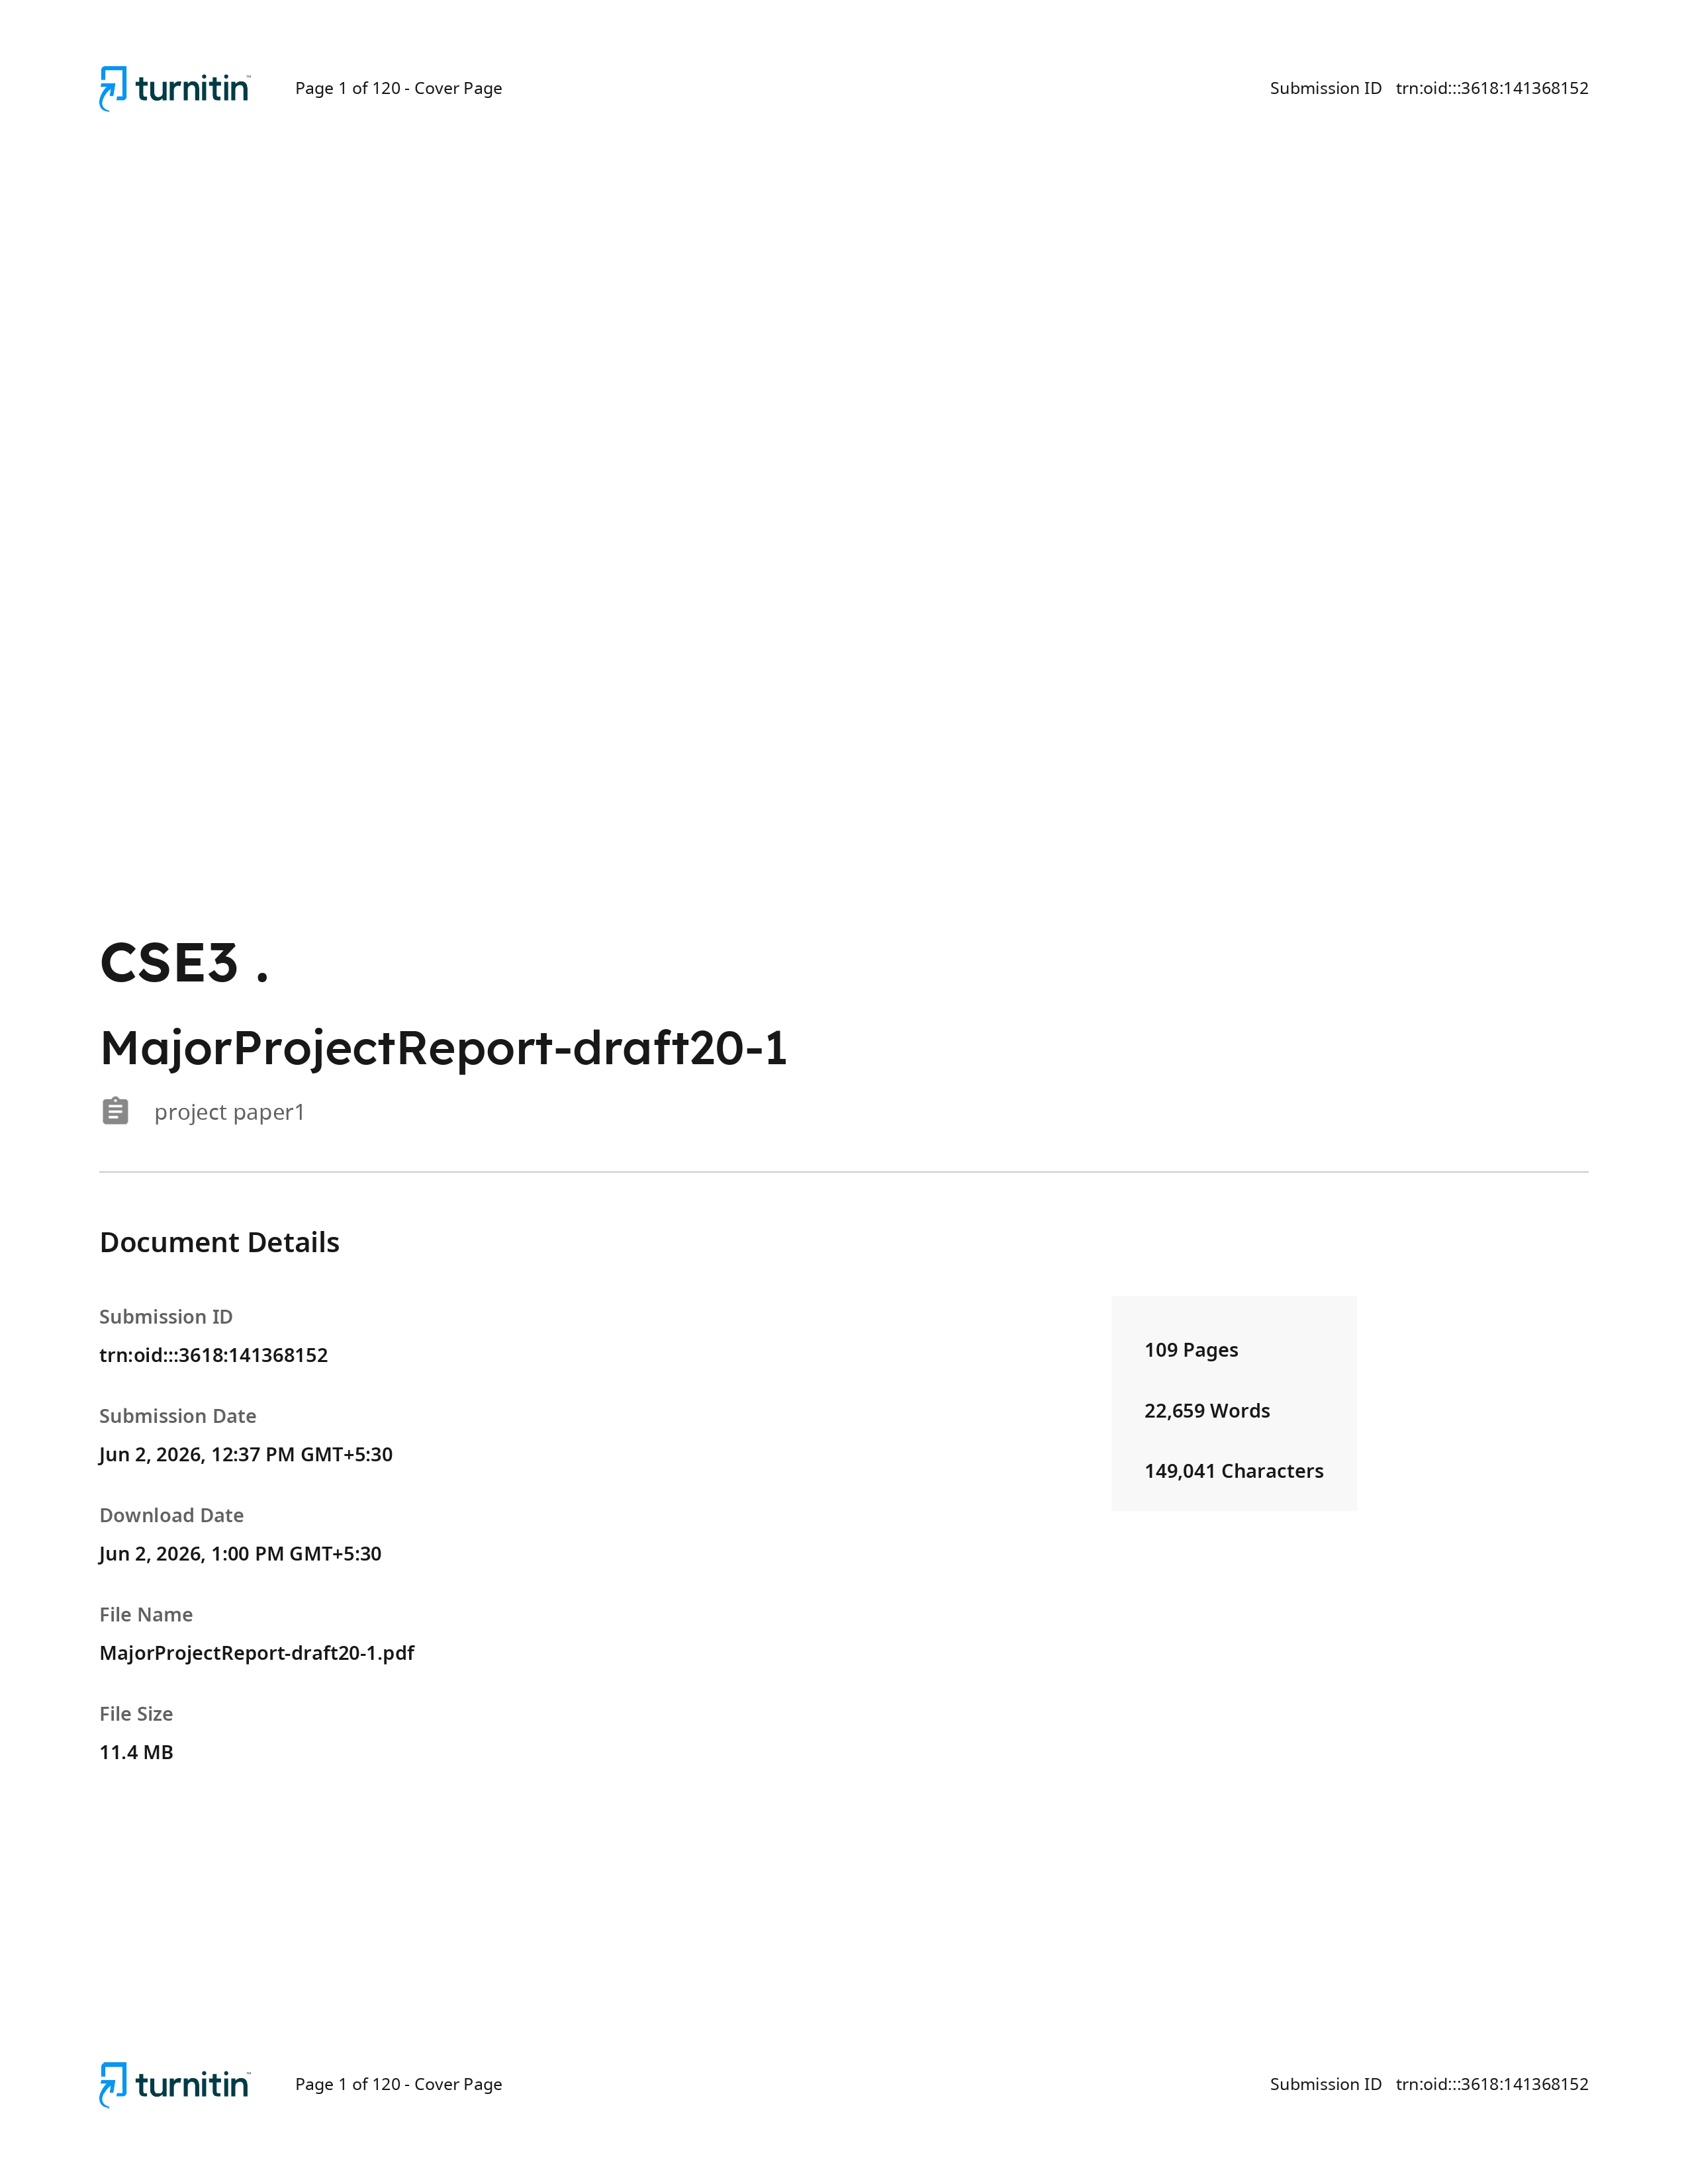
\includegraphics[width=0.9\textwidth]{Appendix/similarity1.jpg}
\caption{Turnitin Similarity Report for the Major Project Report}
\end{figure}

\begin{figure}[H]
\centering
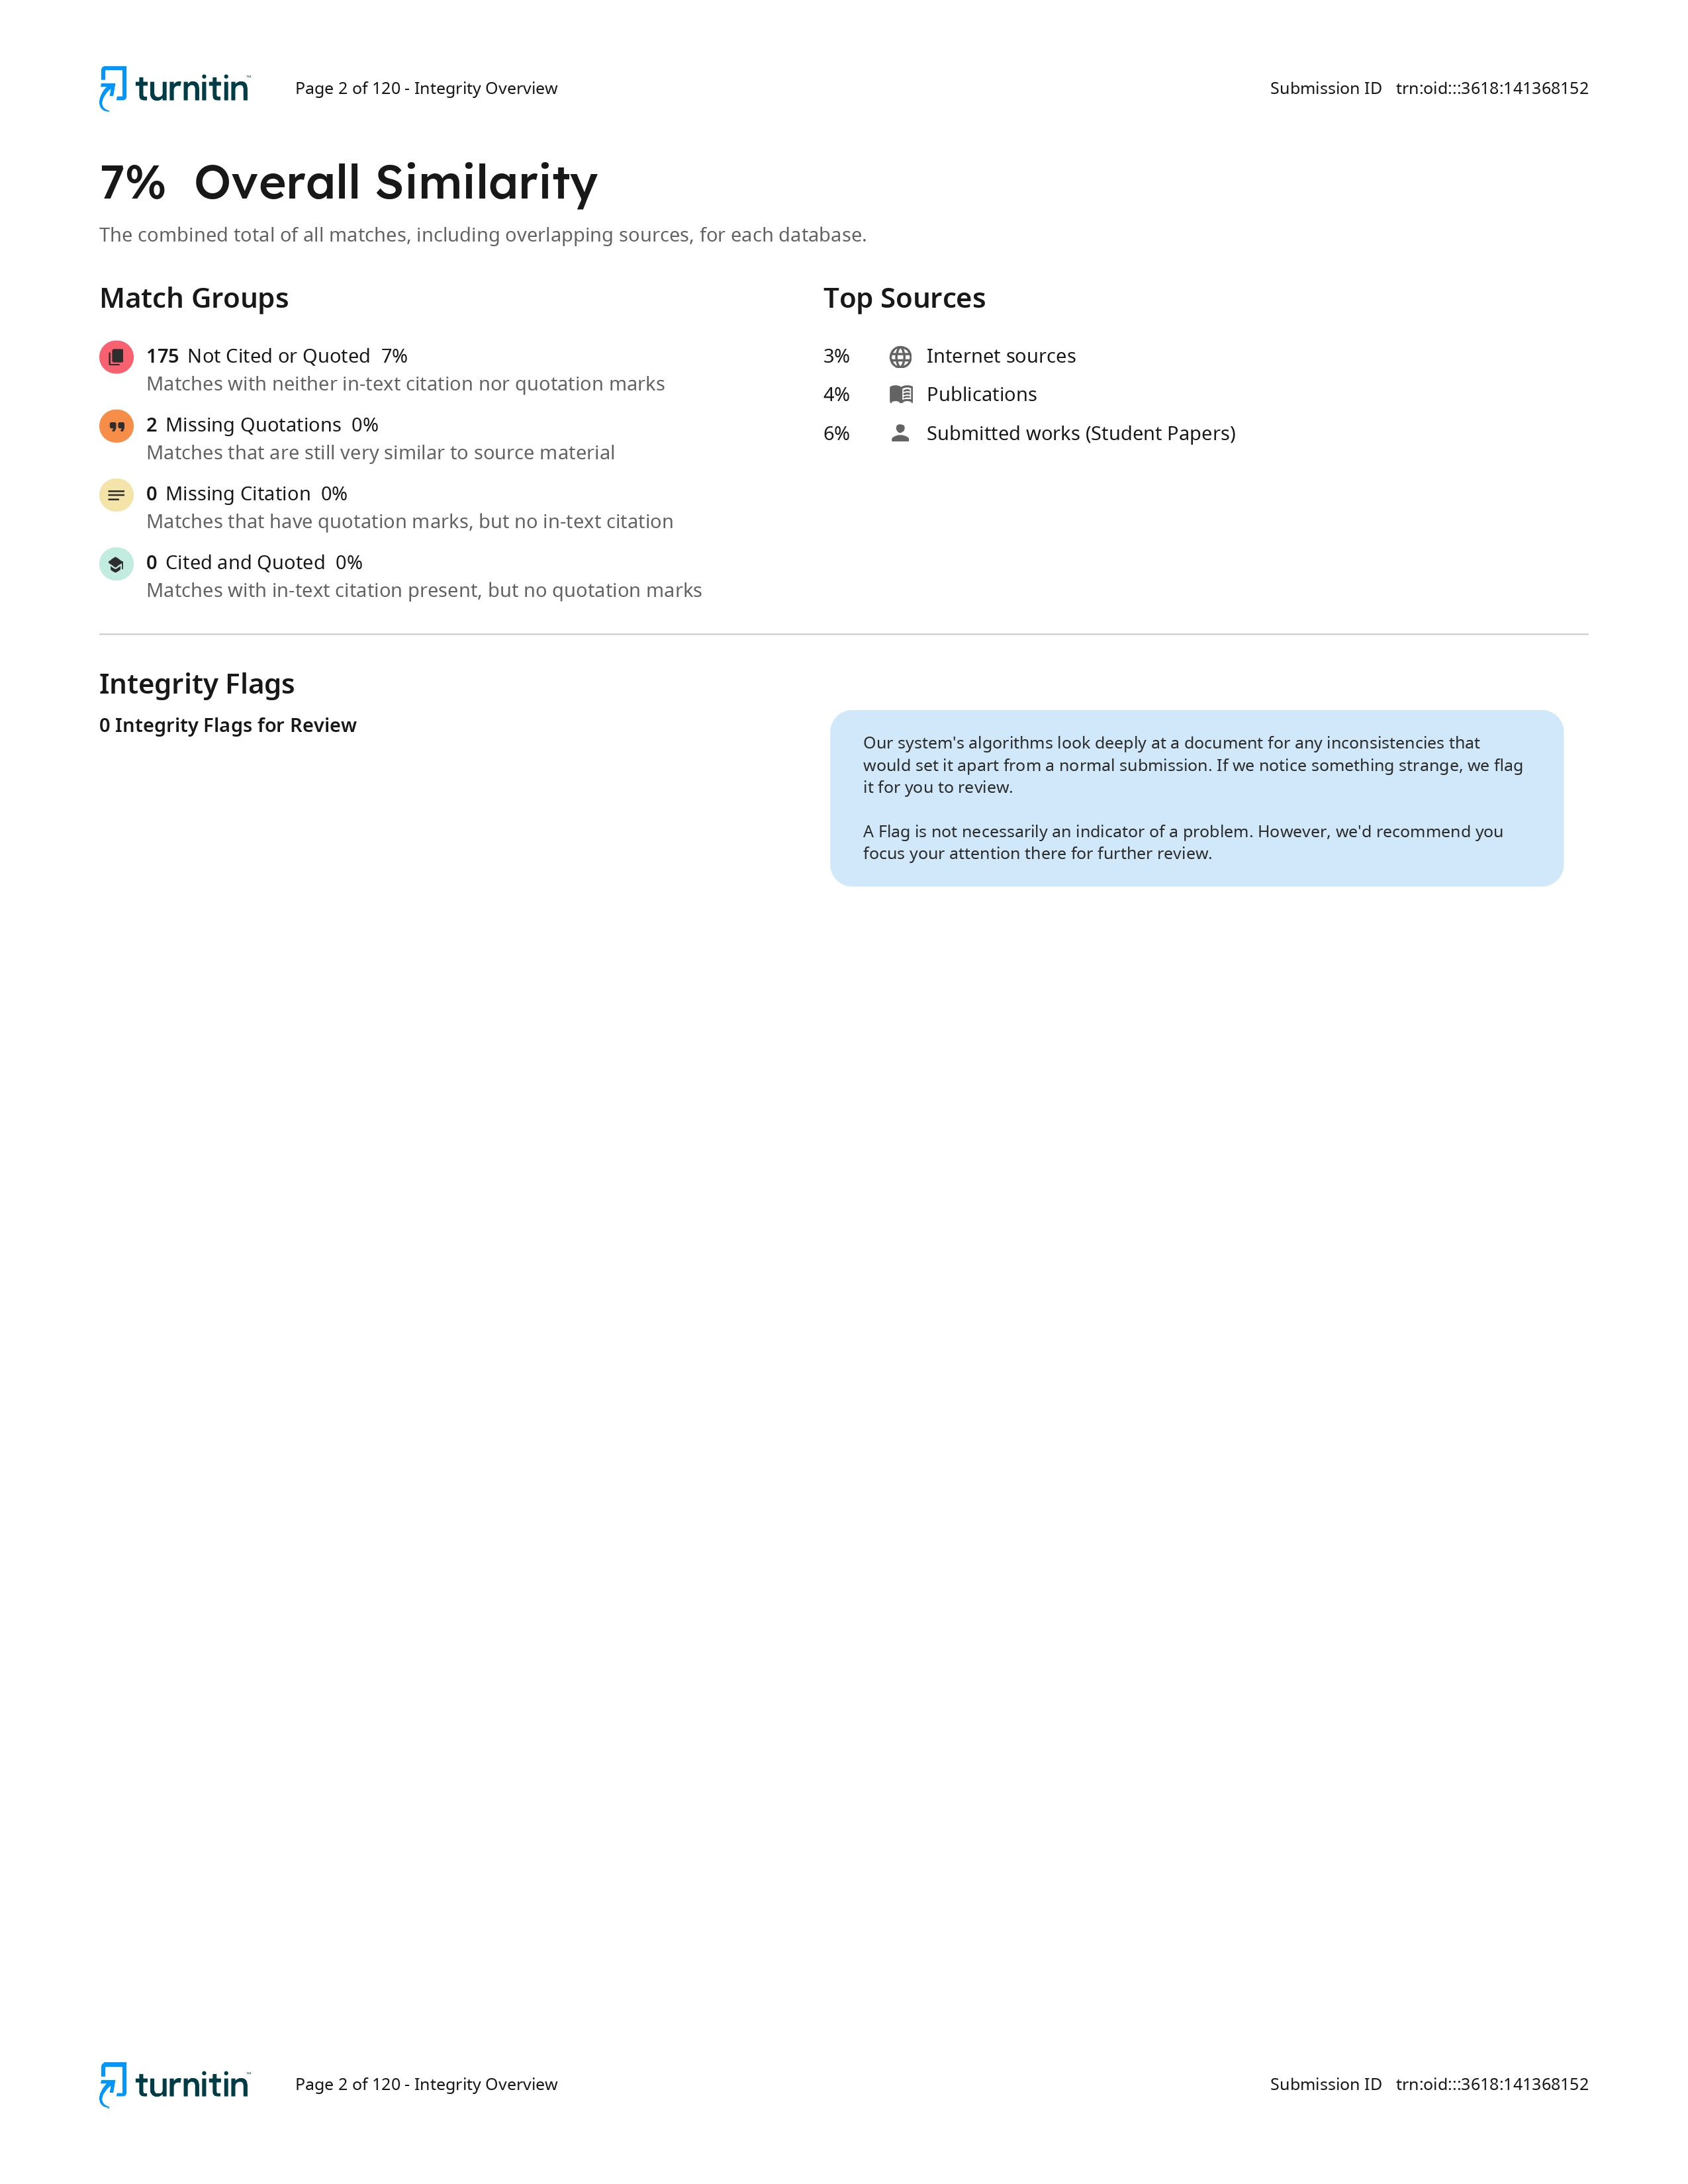
\includegraphics[width=0.9\textwidth]{Appendix/similarity2.jpg}
\caption{Turnitin Similarity Report for the Major Project Report}
\end{figure}


\section{AI Content Detection Report}

\begin{figure}[H]
\centering
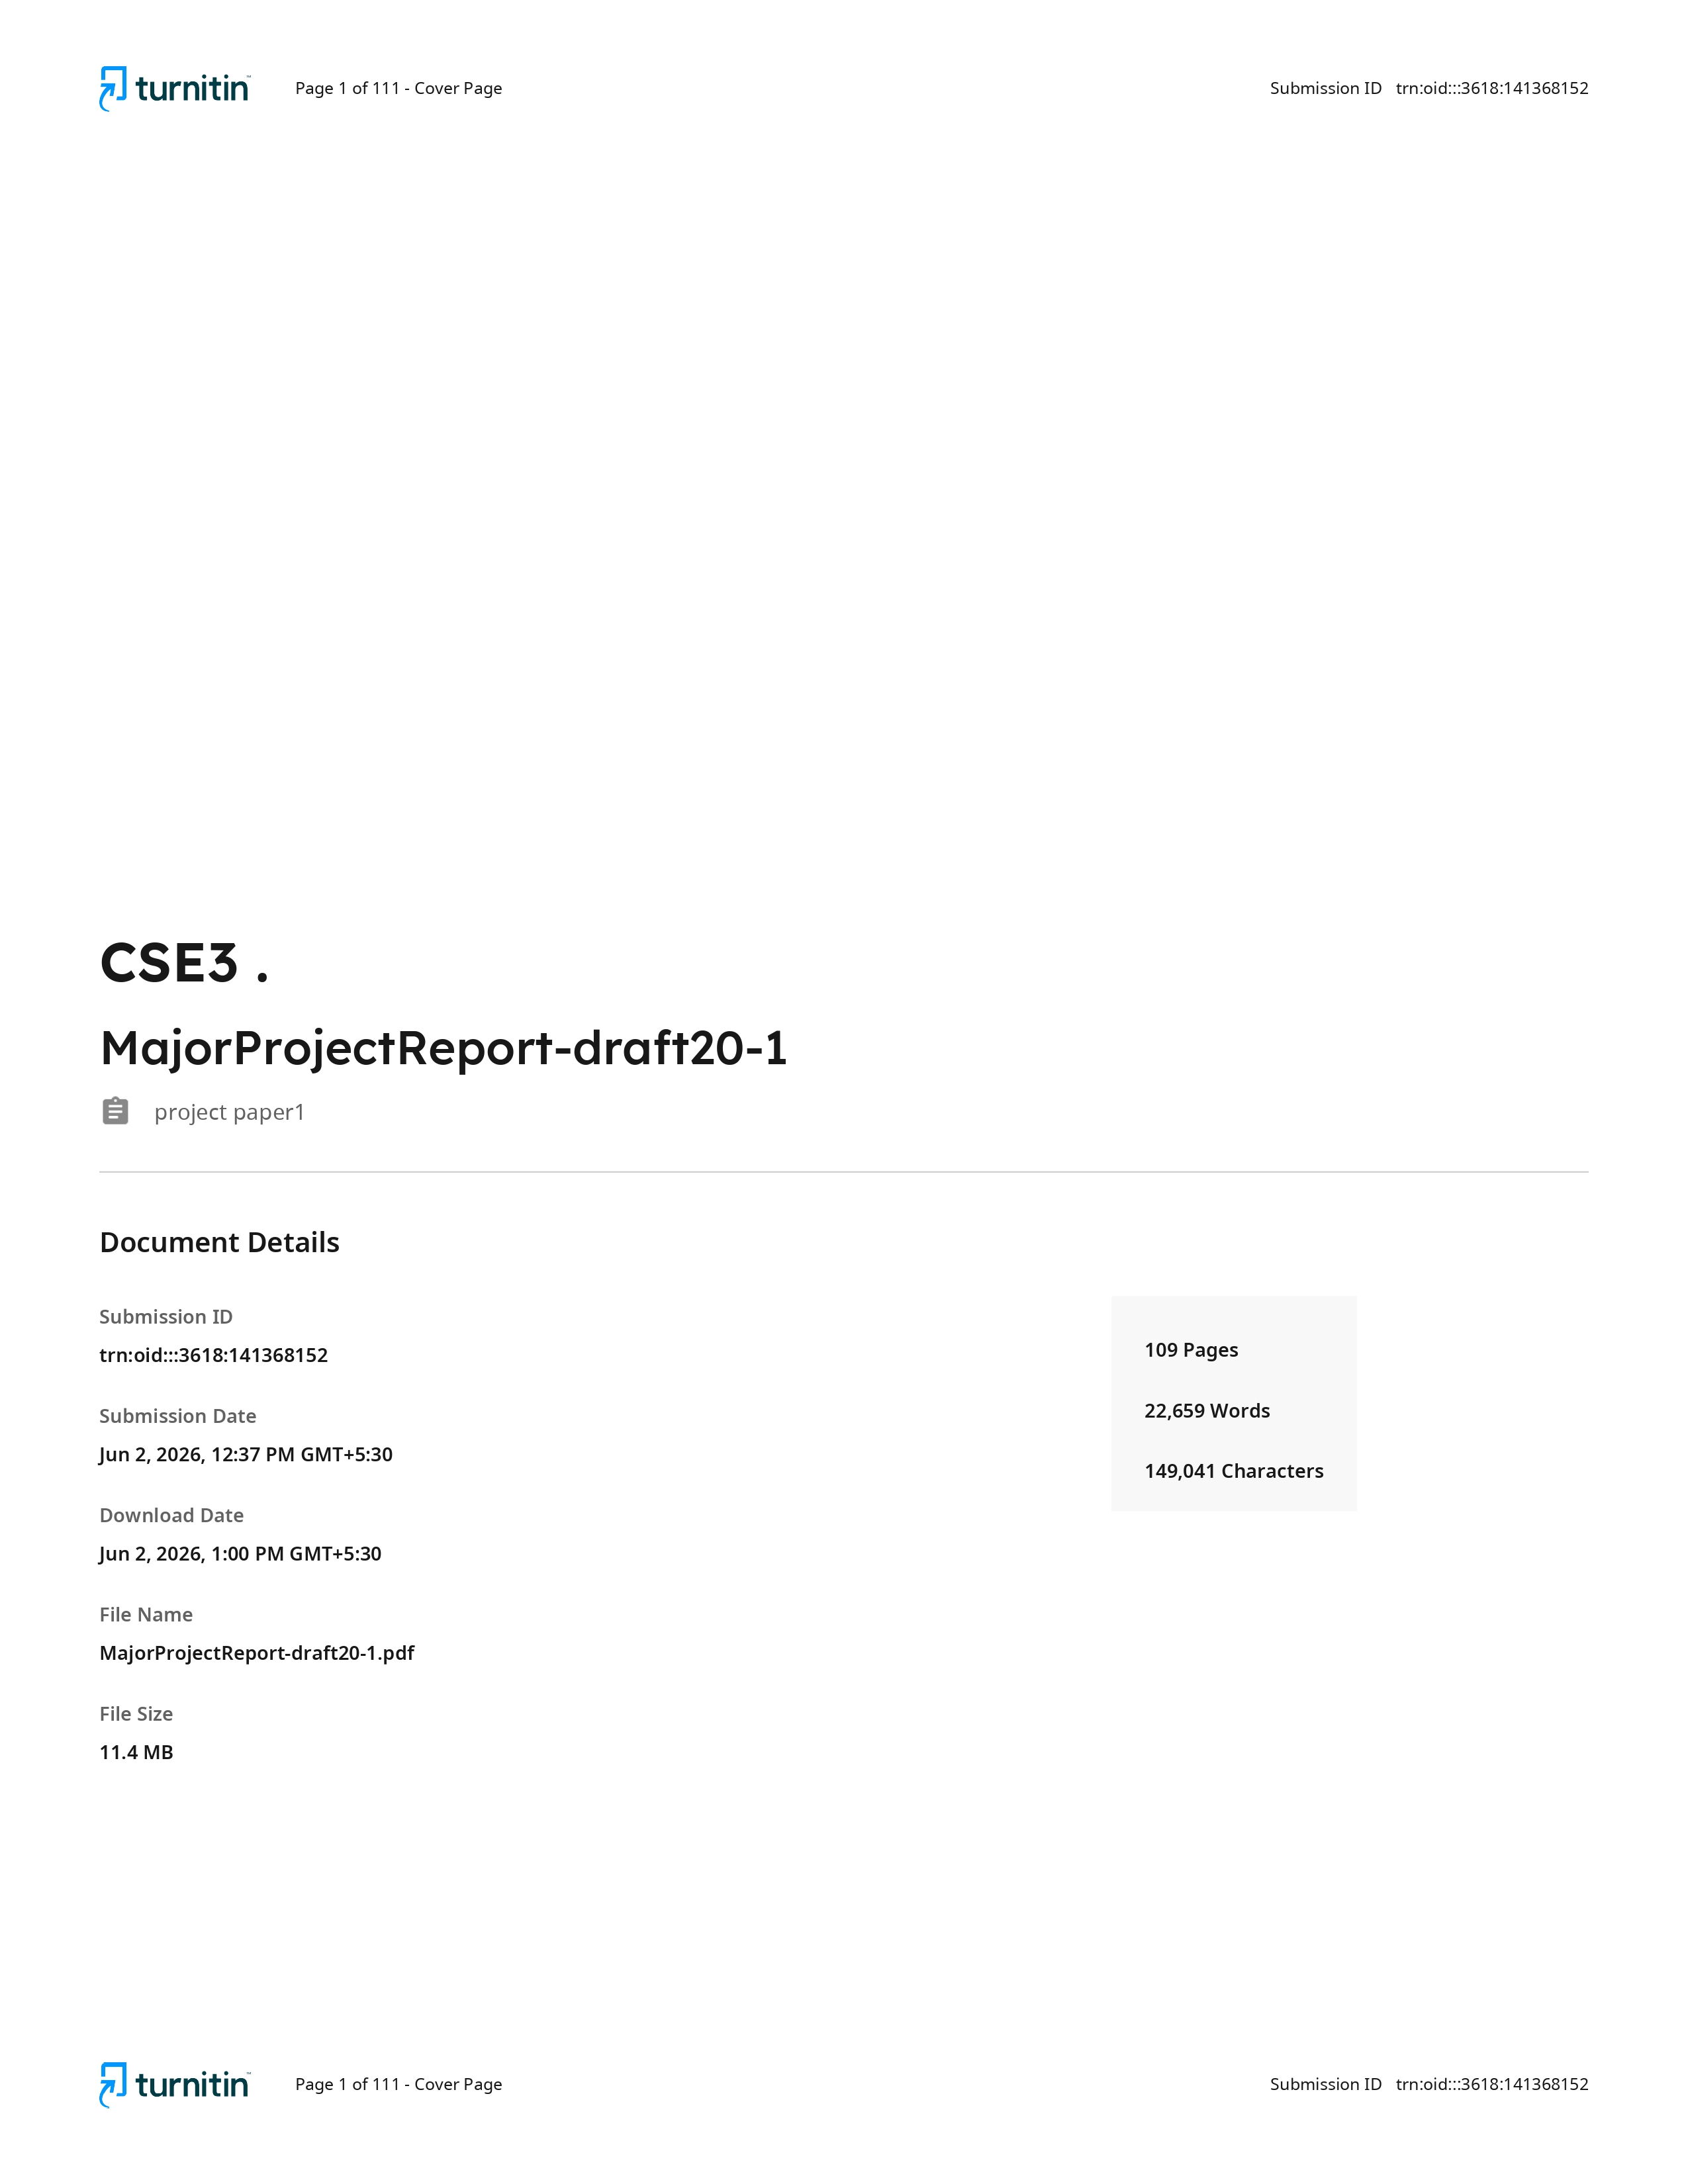
\includegraphics[width=0.9\textwidth]{Appendix/ai1.jpg}
\caption{AI Content Detection Report}
\end{figure}

\begin{figure}[H]
\centering
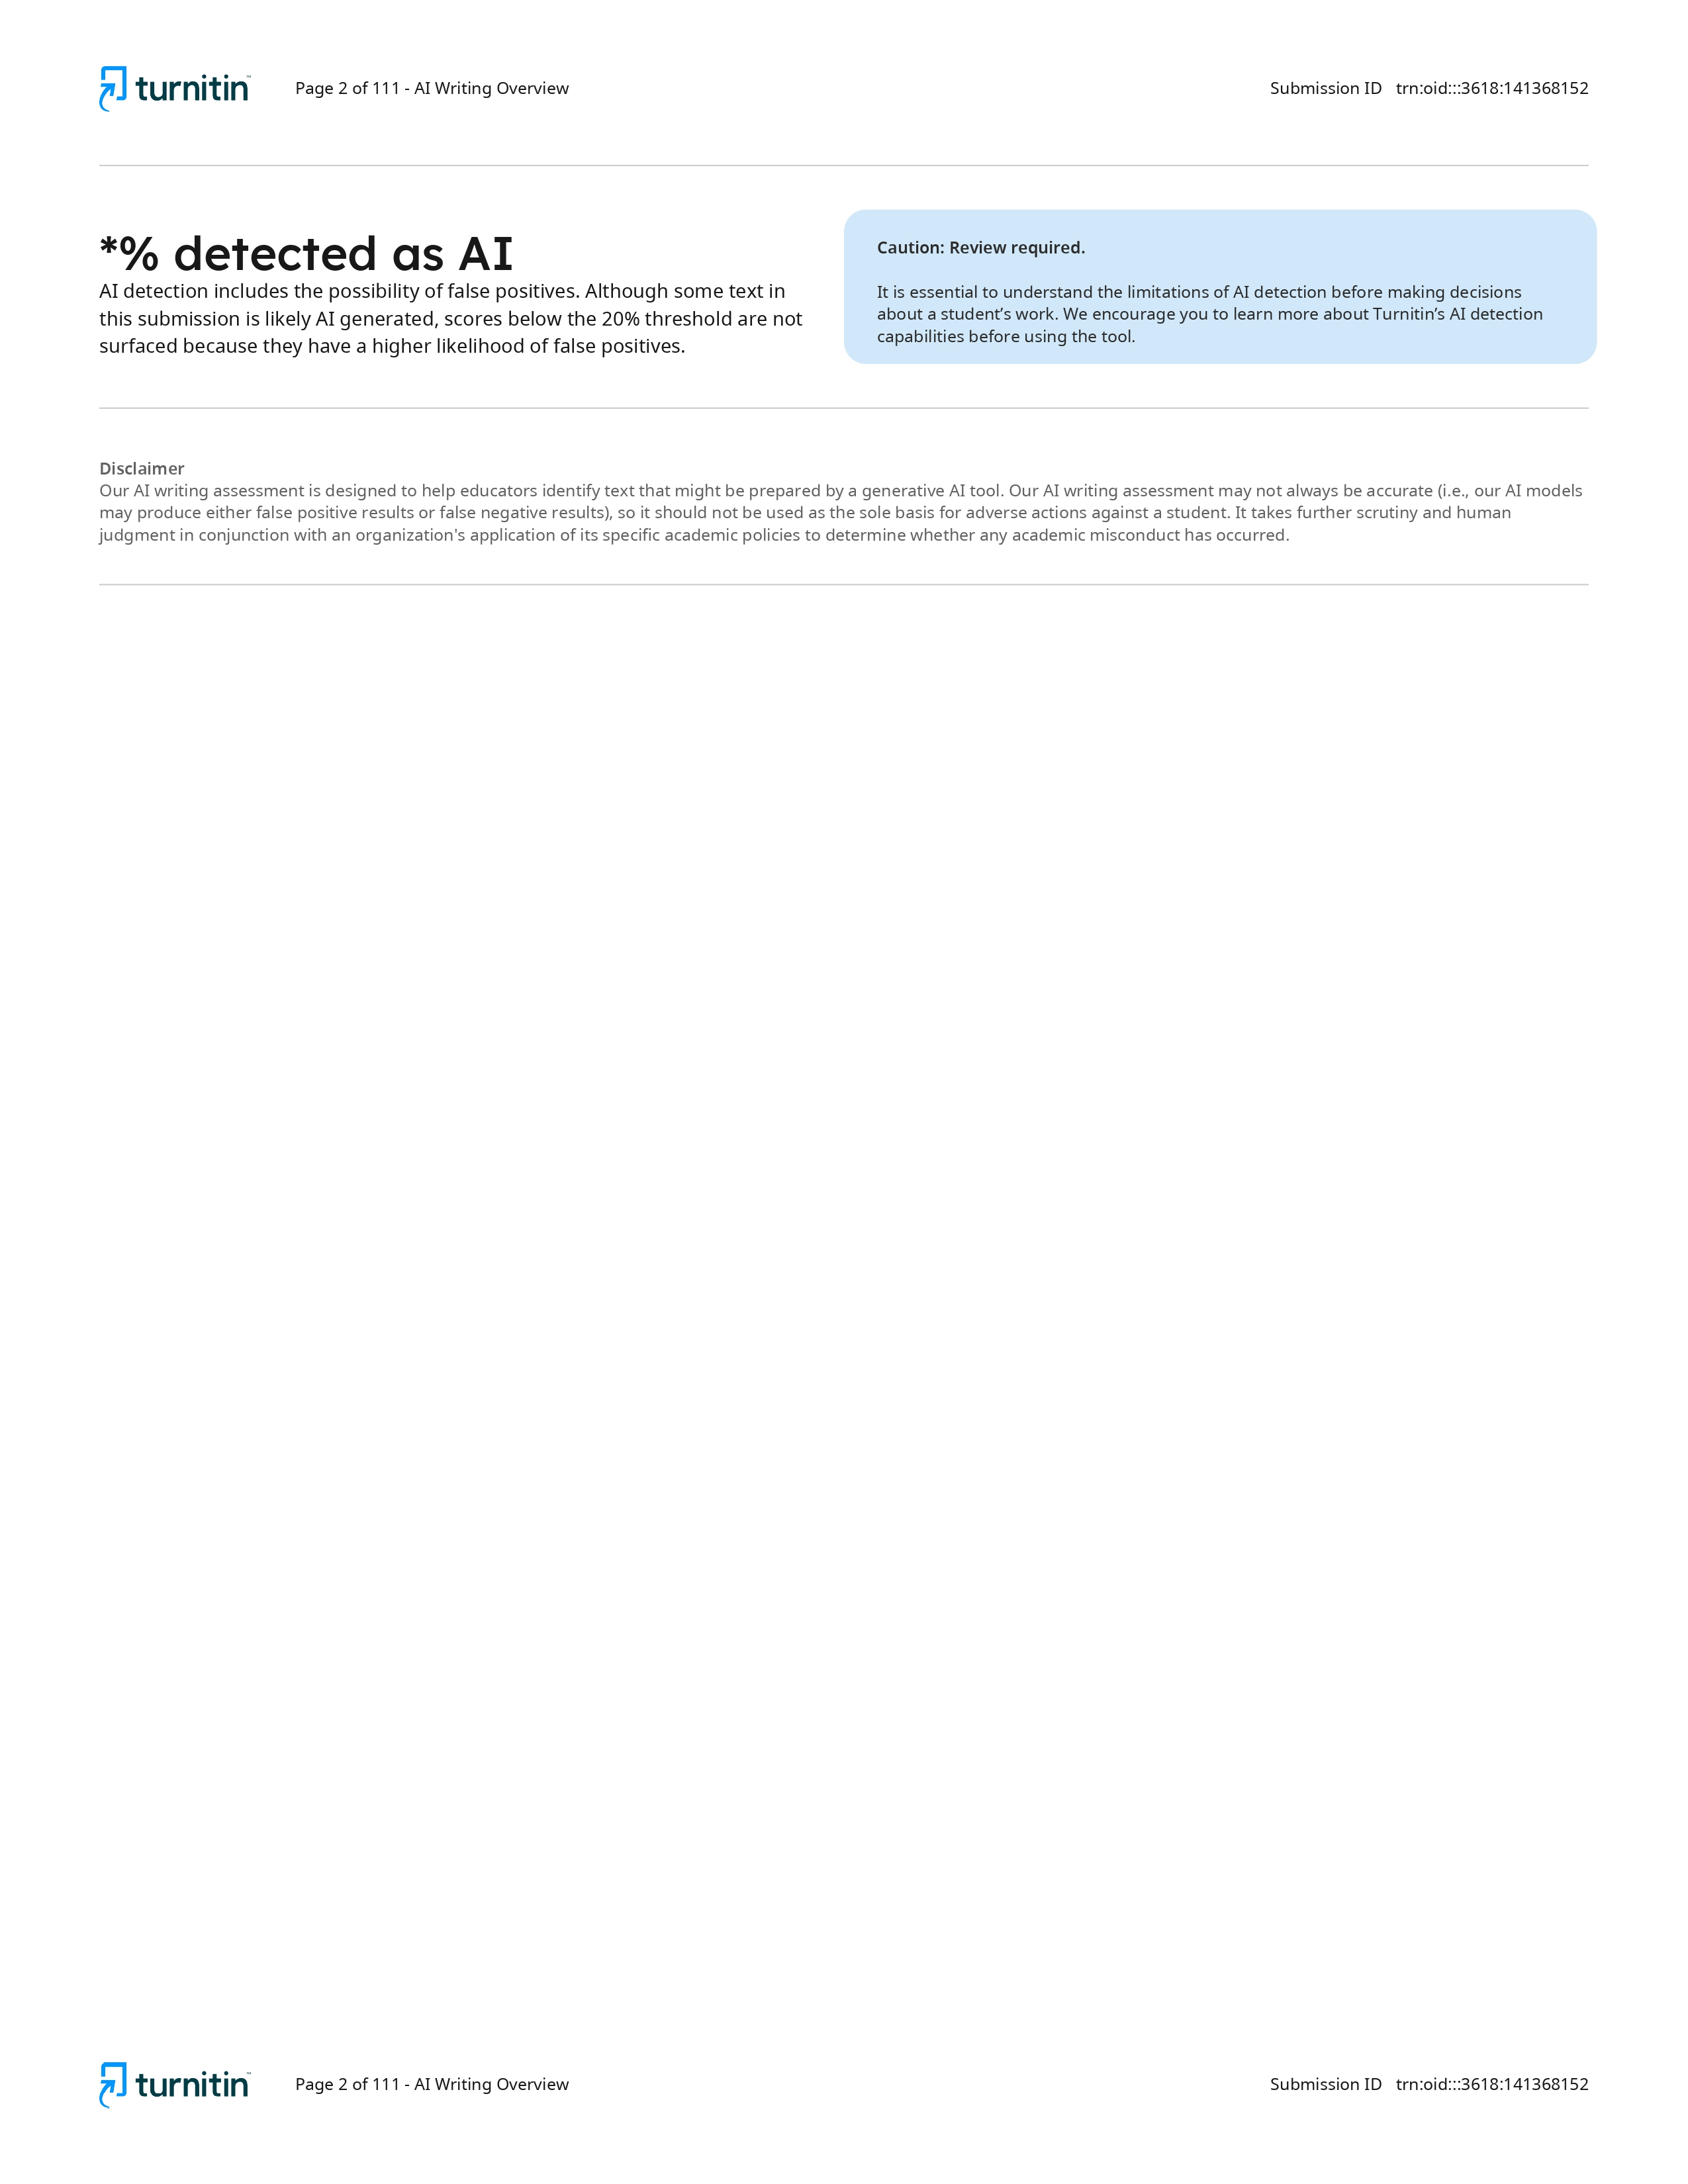
\includegraphics[width=0.9\textwidth]{Appendix/ai2.jpg}
\caption{AI Content Detection Report}
\end{figure}%Appendix Chapter 1
		\chapter{Publication Details}

\section{Journal Manuscript Submission}

\begin{table}[H]
\centering
\renewcommand{\arraystretch}{1.3}
\begin{tabular}{|p{4cm}|p{10cm}|}
\hline
\textbf{Publication Type} & \textbf{Publication Details} \\
\hline
Journal Submission &
``FedGAT--TBML: A Federated Graph Attention Framework for Real-Time Trade-Based Money Laundering Detection,''
submitted to \textit{Discover Artificial Intelligence},
Springer Nature, June 2026. (Under Review). \\
\hline
\end{tabular}
\caption{Details of the submitted journal manuscript.}
\label{tab:publication_details}
\end{table}

\section{Proof of Manuscript Submission}

Figure~\ref{fig:journal_submission} shows the acknowledgment email received from the journal confirming the receipt of the submitted manuscript.

\begin{figure}[H]
    \centering
    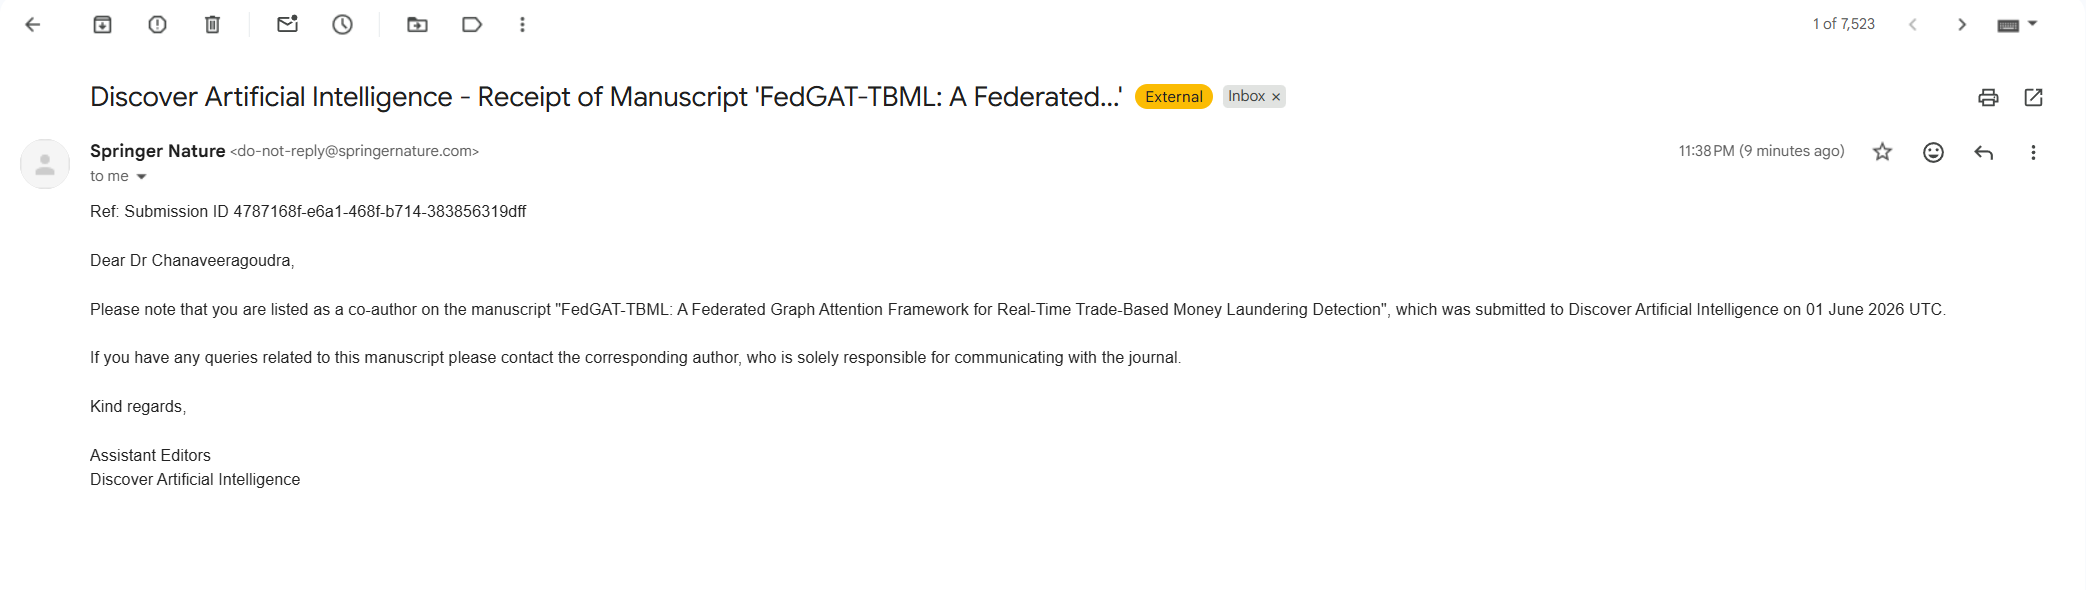
\includegraphics[width=\textwidth]{Appendix/publicationproof.png}
    \caption{Acknowledgment email confirming manuscript submission to Discover Artificial Intelligence (Springer Nature).}
    \label{fig:journal_submission}
\end{figure}%Appendix Chapter 2
		\chapter{Appendix}

%========================================================
\section{Hybrid HGNN--LSTM Model Implementation}
%========================================================

The following listing presents the implementation of the proposed Hybrid HGNN--LSTM analytical model developed using PyTorch and PyTorch Geometric for federated Trade-Based Money Laundering detection.

\begin{tcblisting}{
listing only,
breakable,
colback=gray!10!white,
colframe=black!20,
boxsep=1mm,
left=1mm,
right=1mm,
top=1mm,
bottom=1mm,
listing options={
language=Python,
basicstyle=\scriptsize\ttfamily,
keywordstyle=\color{blue},
commentstyle=\color{gray},
stringstyle=\color{orange},
showstringspaces=false,
breaklines=true,
tabsize=2
}
}

import torch
import torch.nn as nn
import torch.nn.functional as F
from torch_geometric.nn import GATv2Conv, global_mean_pool

class TBML_DetectionModel(nn.Module):

    def __init__(
        self,
        kyc_dim=3,
        swift_dim=1,
        trade_dim=2,
        hidden_dim=32,
        lstm_hidden=32,
        classes=3
    ):

        super(TBML_DetectionModel, self).__init__()

        # Graph Branch

        self.gat1 = GATv2Conv(
            in_channels=kyc_dim,
            out_channels=hidden_dim,
            heads=2,
            concat=False
        )

        self.gat2 = GATv2Conv(
            in_channels=hidden_dim,
            out_channels=hidden_dim,
            heads=2,
            concat=False
        )

        self.gat3 = GATv2Conv(
            in_channels=hidden_dim,
            out_channels=hidden_dim,
            heads=2,
            concat=False
        )

        # Temporal Branch

        self.lstm = nn.LSTM(
            input_size=hidden_dim + swift_dim,
            hidden_size=lstm_hidden,
            batch_first=True
        )

        # Trade Branch

        self.trade_mlp = nn.Sequential(

            nn.Linear(trade_dim, 32),
            nn.LayerNorm(32),
            nn.ReLU(),
            nn.Dropout(0.2),

            nn.Linear(32, 32),
            nn.LayerNorm(32),
            nn.ReLU()

        )

        # Fusion Classifier

        self.classifier = nn.Sequential(

            nn.Linear(lstm_hidden + 32, 64),
            nn.LayerNorm(64),
            nn.ReLU(),
            nn.Dropout(0.2),

            nn.Linear(64, classes)

        )

    def forward(
        self,
        kyc_x,
        edge_index,
        swift_edge_attr,
        seq_data,
        trade_features
    ):

        # Graph Processing

        if edge_index.size(1) == 0:

            enriched_nodes = F.relu(
                self.gat1(kyc_x, edge_index)
            )

        else:

            x = F.dropout(
                F.relu(self.gat1(kyc_x, edge_index)),
                p=0.2,
                training=self.training
            )

            x = F.dropout(
                F.relu(self.gat2(x, edge_index)),
                p=0.2,
                training=self.training
            )

            enriched_nodes = F.dropout(
                F.relu(self.gat3(x, edge_index)),
                p=0.2,
                training=self.training
            )

        # Graph Pooling

        batch = torch.zeros(
            enriched_nodes.size(0),
            dtype=torch.long,
            device=enriched_nodes.device
        )

        graph_context = global_mean_pool(
            enriched_nodes,
            batch
        ).unsqueeze(1)

        # Sequence Shape Correction

        if seq_data.dim() == 4:
            seq_data = seq_data.squeeze(0)

        # Graph + Sequence Fusion

        graph_context_expanded = graph_context.expand(
            seq_data.size(0),
            seq_data.size(1),
            -1
        )

        combined_seq = torch.cat(
            [seq_data, graph_context_expanded],
            dim=-1
        )

        # Temporal Modeling

        lstm_out, _ = self.lstm(combined_seq)

        final_lstm_step = lstm_out[:, -1, :]

        final_lstm_step = F.dropout(
            final_lstm_step,
            p=0.3,
            training=self.training
        )

        # Trade Feature Processing

        trade_emb = self.trade_mlp(trade_features)

        # Final Fusion

        fused_vector = torch.cat(
            [final_lstm_step, trade_emb],
            dim=1
        )

        return self.classifier(fused_vector)

\end{tcblisting}


%========================================================
\section{Federated Learning Server Implementation}
%========================================================

The following listing presents the Flower-based federated server implementation used for distributed parameter aggregation and global model synchronization across institutional clients.

\begin{tcblisting}{
listing only,
breakable,
colback=gray!10!white,
colframe=black!20,
boxsep=1mm,
left=1mm,
right=1mm,
top=1mm,
bottom=1mm,
listing options={
language=Python,
basicstyle=\scriptsize\ttfamily,
keywordstyle=\color{blue},
commentstyle=\color{gray},
stringstyle=\color{orange},
showstringspaces=false,
breaklines=true,
tabsize=2
}
}

import numpy as numpy
import flwr as flwr

from model import TBML_DetectionModel


class modelStrategy(flwr.server.strategy.FedAvg):

    def aggregate_fit(
        self,
        curr_round,
        results,
        failures
    ):

        aggregated_weights, _ = super().aggregate_fit(
            curr_round,
            results,
            failures
        )

        if aggregated_weights is not None and curr_round == 10:

            print(
                f"Saving global weights for round {curr_round}"
            )

            # Convert Flower parameters to NumPy arrays

            aggregated_array = (
                flwr.common.parameters_to_ndarrays(
                    aggregated_weights
                )
            )

            # Save aggregated global weights

            numpy.savez(
                "global_model.npz",
                *aggregated_array
            )

            print(
                "Global weights saved successfully"
            )

        return aggregated_weights, _


if __name__ == "__main__":

    print(
        "Starting Flower server with custom strategy..."
    )

    # Initialize server-side model

    model = TBML_DetectionModel(
        kyc_dim=3,
        swift_dim=1,
        trade_dim=2,
        hidden_dim=32,
        lstm_hidden=32,
        classes=3
    )

    # Convert model weights to Flower parameters

    ndarrays = [

        val.cpu().numpy()

        for val in model.state_dict().values()

    ]

    initial_parameters = (
        flwr.common.ndarrays_to_parameters(
            ndarrays
        )
    )

    # Federated aggregation strategy

    strategy = modelStrategy(

        fraction_fit=1.0,
        min_fit_clients=3,
        min_available_clients=3,
        initial_parameters=initial_parameters

    )

    # Start Flower federated server

    flwr.server.start_server(

        server_address="0.0.0.0:8085",

        config=flwr.server.ServerConfig(
            num_rounds=10
        ),

        strategy=strategy

    )

\end{tcblisting}


%========================================================
\section{Federated Learning Client Implementation}
%========================================================

The following listing presents the Flower federated client implementation used for distributed institutional training, graph-based transaction processing, and federated evaluation within the proposed TBML detection framework.

\begin{tcblisting}{
listing only,
breakable,
colback=gray!10!white,
colframe=black!20,
boxsep=1mm,
left=1mm,
right=1mm,
top=1mm,
bottom=1mm,
listing options={
language=Python,
basicstyle=\scriptsize\ttfamily,
keywordstyle=\color{blue},
commentstyle=\color{gray},
stringstyle=\color{orange},
showstringspaces=false,
breaklines=true,
tabsize=2
}
}

import flwr as fl
import torch
import torch.nn as nn
import torch.optim as optim

from torch.utils.data import Dataset, DataLoader
from torch_geometric.nn import GATv2Conv, global_mean_pool

from neo4j import GraphDatabase
from collections import OrderedDict, Counter

import argparse
import random
import numpy as np

from model import TBML_DetectionModel

SEED = 42

torch.manual_seed(SEED)
np.random.seed(SEED)
random.seed(SEED)

# Client Configuration

parser = argparse.ArgumentParser()

parser.add_argument(
    "--bank",
    type=str,
    required=True,
    choices=['banka', 'bankb', 'bankc']
)

args = parser.parse_args()

PORT_MAP = {

    "banka": 4000,
    "bankb": 4001,
    "bankc": 4002

}

MEMGRAPH_URI = (
    f"bolt://localhost:{PORT_MAP[args.bank]}"
)

MEMGRAPH_USER = ""
MEMGRAPH_PASS = ""

# Dataset Loader

class MemgraphTBMLDataset(Dataset):

    def __init__(
        self,
        uri,
        user,
        password,
        transaction_ids
    ):

        self.driver = GraphDatabase.driver(
            uri,
            auth=(user, password)
        )

        self.transaction_ids = transaction_ids

    def __len__(self):

        return len(self.transaction_ids)

    def __getitem__(self, idx):

        target_msg_id = self.transaction_ids[idx]

        query = """
        MATCH (root:Transaction {id: $target_msg_id})
        OPTIONAL MATCH (root)-[:HAS_DOC]->(trade:Document)

        WITH root, trade

        MATCH (root)-[r1]-(n1:Account)

        WITH root, trade,
             collect(r1) as edges1,
             collect(n1) as nodes1

        UNWIND nodes1 as n1

        OPTIONAL MATCH (n1)-[r2]-(n2:Transaction)

        WITH root, trade,
             edges1,
             nodes1,
             collect(r2)[..50] as edges2,
             collect(n2)[..50] as nodes2

        WITH root, trade,
             nodes1 + [x IN nodes2
             WHERE x IS NOT NULL] AS all_nodes,

             edges1 + [x IN edges2
             WHERE x IS NOT NULL] AS all_edges

        UNWIND all_nodes AS n
        UNWIND all_edges AS r

        RETURN root,
               trade,
               collect(distinct n) AS nodes,
               collect(distinct r) AS edges
        """

        with self.driver.session() as session:

            result = session.run(
                query,
                target_msg_id=target_msg_id
            ).single()

        root = result["root"]
        trade = result["trade"]

        all_nodes_dict = {

            root.element_id: root

        }

        if trade:

            all_nodes_dict[
                trade.element_id
            ] = trade

        for n in result["nodes"]:

            all_nodes_dict[
                n.element_id
            ] = n

        nodes = list(all_nodes_dict.values())

        node_to_idx = {}
        kyc_features = []

        for i, node in enumerate(nodes):

            node_to_idx[node.element_id] = i

            if "Account" in node.labels:

                kyc = [

                    float(node.get("is_shell", 0)),
                    float(node.get("dorm_days", 0))/365.0,
                    float(node.get("device_entropy", 0))

                ]

            else:

                kyc = [0.0, 0.0, 0.0]

            kyc_features.append(kyc)

        kyc_x = torch.tensor(
            kyc_features,
            dtype=torch.float32
        )

        source_nodes = []
        target_nodes = []

        for edge in result["edges"]:

            start_id = edge.start_node.element_id
            end_id = edge.end_node.element_id

            if start_id in node_to_idx and end_id in node_to_idx:

                source_nodes.append(
                    node_to_idx[start_id]
                )

                target_nodes.append(
                    node_to_idx[end_id]
                )

        if len(source_nodes) == 0:

            edge_index = torch.empty(
                (2, 0),
                dtype=torch.long
            )

        else:

            edge_index = torch.tensor(
                [source_nodes, target_nodes],
                dtype=torch.long
            )

        raw_amount = np.log1p(
            float(root.get("amount", 0))
        )

        swift_edge_attr = torch.tensor(
            [[raw_amount]],
            dtype=torch.float32
        )

        seq_data = swift_edge_attr.unsqueeze(0)

        if trade:

            trade_features = torch.tensor([

                float(trade.get(
                    "price_deviation", 0.0
                )),

                float(trade.get(
                    "weight_gap_score", 0.0
                ))

            ], dtype=torch.float32)

        else:

            trade_features = torch.zeros(
                2,
                dtype=torch.float32
            )

        label = torch.tensor(
            int(root.get("label", 0)),
            dtype=torch.long
        )

        return (
            kyc_x,
            edge_index,
            swift_edge_attr,
            seq_data,
            trade_features,
            label
        )

# Federated Client

class BankClient(fl.client.NumPyClient):

    def __init__(
        self,
        model,
        train_loader,
        test_loader,
        class_weights
    ):

        self.model = model

        self.train_loader = train_loader
        self.test_loader = test_loader

        self.criterion = nn.CrossEntropyLoss(
            weight=class_weights
        )

        self.optimizer = optim.Adam(
            model.parameters(),
            lr=0.001
        )

    def get_parameters(self, config):

        return [

            val.cpu().numpy()

            for _, val in
            self.model.state_dict().items()

        ]

    def set_parameters(self, parameters):

        params_dict = zip(
            self.model.state_dict().keys(),
            parameters
        )

        state_dict = OrderedDict({

            k: torch.tensor(v)

            for k, v in params_dict

        })

        self.model.load_state_dict(
            state_dict,
            strict=True
        )

    def fit(self, parameters, config):

        self.set_parameters(parameters)

        self.model.train()

        for epoch in range(1):

            for (
                kyc_x,
                edge_index,
                swift_edge_attr,
                seq_data,
                trade_features,
                label

            ) in self.train_loader:

                kyc_x = kyc_x[0]
                edge_index = edge_index[0]

                swift_edge_attr = (
                    swift_edge_attr[0]
                )

                label = label[0]

                trade_features = (
                    trade_features[0].unsqueeze(0)
                )

                self.optimizer.zero_grad()

                logits = self.model(

                    kyc_x,
                    edge_index,
                    swift_edge_attr,
                    seq_data,
                    trade_features

                )

                loss = self.criterion(
                    logits,
                    label.unsqueeze(0)
                )

                loss.backward()

                torch.nn.utils.clip_grad_norm_(
                    self.model.parameters(),
                    max_norm=1.0
                )

                self.optimizer.step()

        return (
            self.get_parameters(config={}),
            len(self.train_loader.dataset),
            {}
        )

if __name__ == "__main__":

    train_dataset = MemgraphTBMLDataset(
        MEMGRAPH_URI,
        MEMGRAPH_USER,
        MEMGRAPH_PASS,
        []
    )

    train_loader = DataLoader(
        train_dataset,
        batch_size=1,
        shuffle=True
    )

    test_loader = DataLoader(
        train_dataset,
        batch_size=1,
        shuffle=False
    )

    model = TBML_DetectionModel()

    class_weights = torch.tensor(
        [1.0, 1.0, 1.0],
        dtype=torch.float32
    )

    client = BankClient(
        model,
        train_loader,
        test_loader,
        class_weights
    )

    fl.client.start_numpy_client(
        server_address="127.0.0.1:8085",
        client=client
    )

\end{tcblisting}
%Appendix Chapter 3
		
	\end{spacing}
\end{document}
